%%%%%%%%%%%%%%%%%%%%%%%%%%%%%%%%%%%%%%%%%
%  Course Note: MATH2023, 2021 Fall Semester, HKUST
%  Written by: enor2017
%
%  Below is the license of original template I adapted from.
%
% The Legrand Orange Book
% LaTeX Template
% Version 2.4 (26/09/2018)
%
% This template was downloaded from:
% http://www.LaTeXTemplates.com
%
% Original author:
% Mathias Legrand (legrand.mathias@gmail.com) with modifications by:
% Vel (vel@latextemplates.com)
%
% License:
% CC BY-NC-SA 3.0 (http://creativecommons.org/licenses/by-nc-sa/3.0/)
%
%
% Important note:
% Chapter heading images should have a 2:1 width:height ratio,
% e.g. 920px width and 460px height.
%
%%%%%%%%%%%%%%%%%%%%%%%%%%%%%%%%%%%%%%%%%

%----------------------------------------------------------------------------------------
%	PACKAGES AND OTHER DOCUMENT CONFIGURATIONS
%----------------------------------------------------------------------------------------

\documentclass[11pt,fleqn]{book} % Default font size and left-justified equations

%%%%%%%%%%%%%%%%%%%%%%%%%%%%%%%%%%%%%%%%%
% The Legrand Orange Book
% Structural Definitions File
% Version 2.1 (26/09/2018)
%
% Original author:
% Mathias Legrand (legrand.mathias@gmail.com) with modifications by:
% Vel (vel@latextemplates.com)
% 
% This file was downloaded from:
% http://www.LaTeXTemplates.com
%
% License:
% CC BY-NC-SA 3.0 (http://creativecommons.org/licenses/by-nc-sa/3.0/)
%
%%%%%%%%%%%%%%%%%%%%%%%%%%%%%%%%%%%%%%%%%

%----------------------------------------------------------------------------------------
%	VARIOUS REQUIRED PACKAGES AND CONFIGURATIONS
%----------------------------------------------------------------------------------------

\usepackage{graphicx} % Required for including pictures
\graphicspath{{Pictures/}} % Specifies the directory where pictures are stored

\usepackage{lipsum} % Inserts dummy text

\usepackage{tikz} % Required for drawing custom shapes

\usepackage[english]{babel} % English language/hyphenation

\usepackage{enumitem} % Customize lists
\setlist{nolistsep} % Reduce spacing between bullet points and numbered lists

\usepackage{booktabs} % Required for nicer horizontal rules in tables

\usepackage{xcolor} % Required for specifying colors by name
\definecolor{ocre}{RGB}{243,102,25} % Define the orange color used for highlighting throughout the book


\setcounter{chapter}{-1}

%----------------------------------------------------------------------------------------
%	MARGINS
%----------------------------------------------------------------------------------------

\usepackage{geometry} % Required for adjusting page dimensions and margins

\geometry{
	paper=a4paper, % Paper size, change to letterpaper for US letter size
	top=2.54cm, % Top margin
	bottom=2.54cm, % Bottom margin
	left=2.54cm, % Left margin
	right=2.54cm, % Right margin
	headheight=14pt, % Header height
	footskip=1.4cm, % Space from the bottom margin to the baseline of the footer
	headsep=10pt, % Space from the top margin to the baseline of the header
	%showframe, % Uncomment to show how the type block is set on the page
}
\parskip=12pt

%----------------------------------------------------------------------------------------
%	FONTS
%----------------------------------------------------------------------------------------

\usepackage{avant} % Use the Avantgarde font for headings
%\usepackage{times} % Use the Times font for headings
% \usepackage{mathptmx} % Use the Adobe Times Roman as the default text font together with math symbols from the Sym­bol, Chancery and Com­puter Modern fonts

\usepackage{microtype} % Slightly tweak font spacing for aesthetics
\usepackage[utf8]{inputenc} % Required for including letters with accents
\usepackage[T1]{fontenc} % Use 8-bit encoding that has 256 glyphs

%----------------------------------------------------------------------------------------
%	BIBLIOGRAPHY AND INDEX
%----------------------------------------------------------------------------------------

\usepackage[style=numeric,citestyle=numeric,sorting=nyt,sortcites=true,autopunct=true,babel=hyphen,hyperref=true,abbreviate=false,backref=true,backend=biber]{biblatex}
\addbibresource{bibliography.bib} % BibTeX bibliography file
\defbibheading{bibempty}{}

\usepackage{calc} % For simpler calculation - used for spacing the index letter headings correctly
\usepackage{makeidx} % Required to make an index
\makeindex % Tells LaTeX to create the files required for indexing

%----------------------------------------------------------------------------------------
%	MAIN TABLE OF CONTENTS
%----------------------------------------------------------------------------------------

\usepackage{titletoc} % Required for manipulating the table of contents

\contentsmargin{0cm} % Removes the default margin

% Part text styling (this is mostly taken care of in the PART HEADINGS section of this file)
\titlecontents{part}
	[0cm] % Left indentation
	{\addvspace{20pt}\bfseries} % Spacing and font options for parts
	{}
	{}
	{}

% Chapter text styling
\titlecontents{chapter}
	[0cm] % Left indentation
	{\addvspace{12pt}\large\sffamily\bfseries} % Spacing and font options for chapters
	{\color{ocre!60}\contentslabel[\Large\thecontentslabel]{1.25cm}\color{ocre}} % Formatting of numbered sections of this type
	{\color{ocre}} % Formatting of numberless sections of this type
	{\color{ocre!60}\normalsize\;\titlerule*[.5pc]{.}\;\thecontentspage} % Formatting of the filler to the right of the heading and the page number

% Section text styling
\titlecontents{section}
	[0cm] % Left indentation
	{\addvspace{3pt}\sffamily\bfseries} % Spacing and font options for sections
	{\contentslabel[\thecontentslabel]{1.25cm}} % Formatting of numbered sections of this type
	{} % Formatting of numberless sections of this type
	{\hfill\color{black}\thecontentspage} % Formatting of the filler to the right of the heading and the page number

% Subsection text styling
\titlecontents{subsection}
	[0cm] % Left indentation
	{\addvspace{1pt}\sffamily\small} % Spacing and font options for subsections
	{\contentslabel[\thecontentslabel]{1.25cm}} % Formatting of numbered sections of this type
	{} % Formatting of numberless sections of this type
	{\ \titlerule*[.5pc]{.}\;\thecontentspage} % Formatting of the filler to the right of the heading and the page number

% Figure text styling
\titlecontents{figure}
	[1.25cm] % Left indentation
	{\addvspace{1pt}\sffamily\small} % Spacing and font options for figures
	{\thecontentslabel\hspace*{1em}} % Formatting of numbered sections of this type
	{} % Formatting of numberless sections of this type
	{\ \titlerule*[.5pc]{.}\;\thecontentspage} % Formatting of the filler to the right of the heading and the page number

% Table text styling
\titlecontents{table}
	[1.25cm] % Left indentation
	{\addvspace{1pt}\sffamily\small} % Spacing and font options for tables
	{\thecontentslabel\hspace*{1em}} % Formatting of numbered sections of this type
	{} % Formatting of numberless sections of this type
	{\ \titlerule*[.5pc]{.}\;\thecontentspage} % Formatting of the filler to the right of the heading and the page number

%----------------------------------------------------------------------------------------
%	MINI TABLE OF CONTENTS IN PART HEADS
%----------------------------------------------------------------------------------------

% Chapter text styling
\titlecontents{lchapter}
	[0em] % Left indentation
	{\addvspace{15pt}\large\sffamily\bfseries} % Spacing and font options for chapters
	{\color{ocre}\contentslabel[\Large\thecontentslabel]{1.25cm}\color{ocre}} % Chapter number
	{}  
	{\color{ocre}\normalsize\sffamily\bfseries\;\titlerule*[.5pc]{.}\;\thecontentspage} % Page number

% Section text styling
\titlecontents{lsection}
	[0em] % Left indentation
	{\sffamily\small} % Spacing and font options for sections
	{\contentslabel[\thecontentslabel]{1.25cm}} % Section number
	{}
	{}

% Subsection text styling (note these aren't shown by default, display them by searchings this file for tocdepth and reading the commented text)
\titlecontents{lsubsection}
	[0em] % Left indentation
	{\sffamily\footnotesize} % Spacing and font options for subsections
	{\contentslabel[\thecontentslabel]{1.25cm}}
	{}
	{}

%----------------------------------------------------------------------------------------
%	HEADERS AND FOOTERS
%----------------------------------------------------------------------------------------

\usepackage{fancyhdr} % Required for header and footer configuration

\pagestyle{fancy} % Enable the custom headers and footers

\renewcommand{\chaptermark}[1]{\markboth{\sffamily\normalsize\bfseries\chaptername\ \thechapter.\ #1}{}} % Styling for the current chapter in the header
\renewcommand{\sectionmark}[1]{\markright{\sffamily\normalsize\thesection\hspace{5pt}#1}{}} % Styling for the current section in the header

\fancyhf{} % Clear default headers and footers
\fancyhead[LE,RO]{\sffamily\normalsize\thepage} % Styling for the page number in the header
\fancyhead[LO]{\rightmark} % Print the nearest section name on the left side of odd pages
\fancyhead[RE]{\leftmark} % Print the current chapter name on the right side of even pages
%\fancyfoot[C]{\thepage} % Uncomment to include a footer

\renewcommand{\headrulewidth}{0.5pt} % Thickness of the rule under the header

\fancypagestyle{plain}{% Style for when a plain pagestyle is specified
	\fancyhead{}\renewcommand{\headrulewidth}{0pt}%
}

% Removes the header from odd empty pages at the end of chapters
\makeatletter
\renewcommand{\cleardoublepage}{
\clearpage\ifodd\c@page\else
\hbox{}
\vspace*{\fill}
\thispagestyle{empty}
\newpage
\fi}

%----------------------------------------------------------------------------------------
%	THEOREM STYLES
%----------------------------------------------------------------------------------------

\usepackage{amsmath,amsfonts,amssymb,amsthm} % For math equations, theorems, symbols, etc

\newcommand{\intoo}[2]{\mathopen{]}#1\,;#2\mathclose{[}}
\newcommand{\ud}{\mathop{\mathrm{{}d}}\mathopen{}}
\newcommand{\intff}[2]{\mathopen{[}#1\,;#2\mathclose{]}}
\renewcommand{\qedsymbol}{$\blacksquare$}
\newtheorem{notation}{Notation}[chapter]

% Boxed/framed environments
\newtheoremstyle{ocrenumbox}% Theorem style name
{0pt}% Space above
{0pt}% Space below
{\normalfont}% Body font
{}% Indent amount
{\small\bf\sffamily\color{ocre}}% Theorem head font
{\;}% Punctuation after theorem head
{0.25em}% Space after theorem head
{\small\sffamily\color{ocre}\thmname{#1}\nobreakspace\thmnumber{\@ifnotempty{#1}{}\@upn{#2}}% Theorem text (e.g. Theorem 2.1)
\thmnote{\nobreakspace\the\thm@notefont\sffamily\bfseries\color{black}---\nobreakspace#3.}} % Optional theorem note

\newtheoremstyle{blacknumex}% Theorem style name
{5pt}% Space above
{5pt}% Space below
{\normalfont}% Body font
{} % Indent amount
{\small\bf\sffamily}% Theorem head font
{\;}% Punctuation after theorem head
{0.25em}% Space after theorem head
{\small\sffamily{\tiny\ensuremath{\blacksquare}}\nobreakspace\thmname{#1}\nobreakspace\thmnumber{\@ifnotempty{#1}{}\@upn{#2}}% Theorem text (e.g. Theorem 2.1)
\thmnote{\nobreakspace\the\thm@notefont\sffamily\bfseries---\nobreakspace#3.}}% Optional theorem note

\newtheoremstyle{blacknumbox} % Theorem style name
{0pt}% Space above
{0pt}% Space below
{\normalfont}% Body font
{}% Indent amount
{\small\bf\sffamily}% Theorem head font
{\;}% Punctuation after theorem head
{0.25em}% Space after theorem head
{\small\sffamily\thmname{#1}\nobreakspace\thmnumber{\@ifnotempty{#1}{}\@upn{#2}}% Theorem text (e.g. Theorem 2.1)
\thmnote{\nobreakspace\the\thm@notefont\sffamily\bfseries---\nobreakspace#3.}}% Optional theorem note

% Non-boxed/non-framed environments
\newtheoremstyle{ocrenum}% Theorem style name
{5pt}% Space above
{5pt}% Space below
{\normalfont}% Body font
{}% Indent amount
{\small\bf\sffamily\color{ocre}}% Theorem head font
{\;}% Punctuation after theorem head
{0.25em}% Space after theorem head
{\small\sffamily\color{ocre}\thmname{#1}\nobreakspace\thmnumber{\@ifnotempty{#1}{}\@upn{#2}}% Theorem text (e.g. Theorem 2.1)
\thmnote{\nobreakspace\the\thm@notefont\sffamily\bfseries\color{black}---\nobreakspace#3.}} % Optional theorem note
\makeatother

% Defines the theorem text style for each type of theorem to one of the three styles above
\newcounter{dummy} 
\numberwithin{dummy}{section}
\theoremstyle{ocrenumbox}
\newtheorem{theoremeT}[dummy]{Theorem}
\newtheorem{problem}{Problem}[chapter]
\newtheorem{exerciseT}{Exercise}[chapter]
\theoremstyle{blacknumex}
\newtheorem{exampleT}{Example}[chapter]
\theoremstyle{blacknumbox}
\newtheorem{vocabulary}{Vocabulary}[chapter]
\newtheorem{definitionT}{Definition}[section]
\newtheorem{corollaryT}[dummy]{Corollary}
\theoremstyle{ocrenum}
\newtheorem{proposition}[dummy]{Proposition}

%----------------------------------------------------------------------------------------
%	DEFINITION OF COLORED BOXES
%----------------------------------------------------------------------------------------

\RequirePackage[framemethod=default]{mdframed} % Required for creating the theorem, definition, exercise and corollary boxes

% Theorem box
\newmdenv[skipabove=7pt,
skipbelow=7pt,
backgroundcolor=black!5,
linecolor=ocre,
innerleftmargin=5pt,
innerrightmargin=5pt,
innertopmargin=20pt,
leftmargin=0cm,
rightmargin=0cm,
innerbottommargin=10pt]{tBox}

% Exercise box	  
\newmdenv[skipabove=7pt,
skipbelow=7pt,
rightline=false,
leftline=true,
topline=false,
bottomline=false,
backgroundcolor=ocre!10,
linecolor=ocre,
innerleftmargin=5pt,
innerrightmargin=5pt,
innertopmargin=5pt,
innerbottommargin=5pt,
leftmargin=0cm,
rightmargin=0cm,
linewidth=4pt]{eBox}	

% Definition box
\newmdenv[skipabove=7pt,
skipbelow=7pt,
rightline=false,
leftline=true,
topline=false,
bottomline=false,
linecolor=ocre,
innerleftmargin=5pt,
innerrightmargin=5pt,
innertopmargin=18pt,
leftmargin=0cm,
rightmargin=0cm,
linewidth=4pt,
innerbottommargin=10pt]{dBox}	

% Corollary box
\newmdenv[skipabove=7pt,
skipbelow=7pt,
rightline=false,
leftline=true,
topline=false,
bottomline=false,
linecolor=gray,
backgroundcolor=black!5,
innerleftmargin=5pt,
innerrightmargin=5pt,
innertopmargin=5pt,
leftmargin=0cm,
rightmargin=0cm,
linewidth=4pt,
innerbottommargin=5pt]{cBox}

% Creates an environment for each type of theorem and assigns it a theorem text style from the "Theorem Styles" section above and a colored box from above
\newenvironment{theorem}{\begin{tBox}\begin{theoremeT}}{\end{theoremeT}\end{tBox}}
\newenvironment{exercise}{\begin{eBox}\begin{exerciseT}}{\hfill{\color{ocre}\tiny\ensuremath{\blacksquare}}\end{exerciseT}\end{eBox}}				  
\newenvironment{definition}{\begin{dBox}\begin{definitionT}}{\end{definitionT}\end{dBox}}	
\newenvironment{example}{\begin{exampleT}}{\hfill{\tiny\ensuremath{\blacksquare}}\end{exampleT}}		
\newenvironment{corollary}{\begin{cBox}\begin{corollaryT}}{\end{corollaryT}\end{cBox}}	

%----------------------------------------------------------------------------------------
%	REMARK ENVIRONMENT
%----------------------------------------------------------------------------------------

\newenvironment{remark}{\par\vspace{10pt}\small % Vertical white space above the remark and smaller font size
\begin{list}{}{
\leftmargin=25pt % Indentation on the left
\rightmargin=25pt}\item\ignorespaces % Indentation on the right
\makebox[-2.5pt]{\begin{tikzpicture}[overlay]
\node[draw=ocre!60,line width=1pt,circle,fill=ocre!25,font=\sffamily\bfseries,inner sep=2pt,outer sep=0pt] at (-15pt,0pt){\textcolor{ocre}{R}};\end{tikzpicture}} % Orange R in a circle
\advance\baselineskip -1pt}{\end{list}\vskip5pt} % Tighter line spacing and white space after remark

%----------------------------------------------------------------------------------------
%	SECTION NUMBERING IN THE MARGIN
%----------------------------------------------------------------------------------------

\makeatletter
\renewcommand{\@seccntformat}[1]{\llap{\textcolor{ocre}{\csname the#1\endcsname}\hspace{1em}}}                    
\renewcommand{\section}{\@startsection{section}{1}{\z@}
{-4ex \@plus -1ex \@minus -.4ex}
{1ex \@plus.2ex }
{\normalfont\large\sffamily\bfseries}}
\renewcommand{\subsection}{\@startsection {subsection}{2}{\z@}
{-3ex \@plus -0.1ex \@minus -.4ex}
{0.5ex \@plus.2ex }
{\normalfont\sffamily\bfseries}}
\renewcommand{\subsubsection}{\@startsection {subsubsection}{3}{\z@}
{-2ex \@plus -0.1ex \@minus -.2ex}
{.2ex \@plus.2ex }
{\normalfont\small\sffamily\bfseries}}                        
\renewcommand\paragraph{\@startsection{paragraph}{4}{\z@}
{-2ex \@plus-.2ex \@minus .2ex}
{.1ex}
{\normalfont\small\sffamily\bfseries}}

%----------------------------------------------------------------------------------------
%	PART HEADINGS
%----------------------------------------------------------------------------------------

% Numbered part in the table of contents
\newcommand{\@mypartnumtocformat}[2]{%
	\setlength\fboxsep{0pt}%
	\noindent\colorbox{ocre!20}{\strut\parbox[c][.7cm]{\ecart}{\color{ocre!70}\Large\sffamily\bfseries\centering#1}}\hskip\esp\colorbox{ocre!40}{\strut\parbox[c][.7cm]{\linewidth-\ecart-\esp}{\Large\sffamily\centering#2}}%
}

% Unnumbered part in the table of contents
\newcommand{\@myparttocformat}[1]{%
	\setlength\fboxsep{0pt}%
	\noindent\colorbox{ocre!40}{\strut\parbox[c][.7cm]{\linewidth}{\Large\sffamily\centering#1}}%
}

\newlength\esp
\setlength\esp{4pt}
\newlength\ecart
\setlength\ecart{1.2cm-\esp}
\newcommand{\thepartimage}{}%
\newcommand{\partimage}[1]{\renewcommand{\thepartimage}{#1}}%
\def\@part[#1]#2{%
\ifnum \c@secnumdepth >-2\relax%
\refstepcounter{part}%
\addcontentsline{toc}{part}{\texorpdfstring{\protect\@mypartnumtocformat{\thepart}{#1}}{\partname~\thepart\ ---\ #1}}
\else%
\addcontentsline{toc}{part}{\texorpdfstring{\protect\@myparttocformat{#1}}{#1}}%
\fi%
\startcontents%
\markboth{}{}%
{\thispagestyle{empty}%
\begin{tikzpicture}[remember picture,overlay]%
\node at (current page.north west){\begin{tikzpicture}[remember picture,overlay]%	
\fill[ocre!20](0cm,0cm) rectangle (\paperwidth,-\paperheight);
\node[anchor=north] at (4cm,-3.25cm){\color{ocre!40}\fontsize{220}{100}\sffamily\bfseries\thepart}; 
\node[anchor=south east] at (\paperwidth-1cm,-\paperheight+1cm){\parbox[t][][t]{8.5cm}{
\printcontents{l}{0}{\setcounter{tocdepth}{1}}% The depth to which the Part mini table of contents displays headings; 0 for chapters only, 1 for chapters and sections and 2 for chapters, sections and subsections
}};
\node[anchor=north east] at (\paperwidth-1.5cm,-3.25cm){\parbox[t][][t]{15cm}{\strut\raggedleft\color{white}\fontsize{30}{30}\sffamily\bfseries#2}};
\end{tikzpicture}};
\end{tikzpicture}}%
\@endpart}
\def\@spart#1{%
\startcontents%
\phantomsection
{\thispagestyle{empty}%
\begin{tikzpicture}[remember picture,overlay]%
\node at (current page.north west){\begin{tikzpicture}[remember picture,overlay]%	
\fill[ocre!20](0cm,0cm) rectangle (\paperwidth,-\paperheight);
\node[anchor=north east] at (\paperwidth-1.5cm,-3.25cm){\parbox[t][][t]{15cm}{\strut\raggedleft\color{white}\fontsize{30}{30}\sffamily\bfseries#1}};
\end{tikzpicture}};
\end{tikzpicture}}
\addcontentsline{toc}{part}{\texorpdfstring{%
\setlength\fboxsep{0pt}%
\noindent\protect\colorbox{ocre!40}{\strut\protect\parbox[c][.7cm]{\linewidth}{\Large\sffamily\protect\centering #1\quad\mbox{}}}}{#1}}%
\@endpart}
\def\@endpart{\vfil\newpage
\if@twoside
\if@openright
\null
\thispagestyle{empty}%
\newpage
\fi
\fi
\if@tempswa
\twocolumn
\fi}

%----------------------------------------------------------------------------------------
%	CHAPTER HEADINGS
%----------------------------------------------------------------------------------------

% A switch to conditionally include a picture, implemented by Christian Hupfer
\newif\ifusechapterimage
\usechapterimagetrue
\newcommand{\thechapterimage}{}%
\newcommand{\chapterimage}[1]{\ifusechapterimage\renewcommand{\thechapterimage}{#1}\fi}%
\newcommand{\autodot}{.}
\def\@makechapterhead#1{%
{\parindent \z@ \raggedright \normalfont
\ifnum \c@secnumdepth >\m@ne
\if@mainmatter
\begin{tikzpicture}[remember picture,overlay]
\node at (current page.north west)
{\begin{tikzpicture}[remember picture,overlay]
\node[anchor=north west,inner sep=0pt] at (0,0) {\ifusechapterimage\includegraphics[width=\paperwidth]{\thechapterimage}\fi};
\draw[anchor=west] (\Gm@lmargin,-9cm) node [line width=2pt,rounded corners=15pt,draw=ocre,fill=white,fill opacity=0.5,inner sep=15pt]{\strut\makebox[22cm]{}};
\draw[anchor=west] (\Gm@lmargin+.3cm,-9cm) node {\huge\sffamily\bfseries\color{black}\thechapter\autodot~#1\strut};
\end{tikzpicture}};
\end{tikzpicture}
\else
\begin{tikzpicture}[remember picture,overlay]
\node at (current page.north west)
{\begin{tikzpicture}[remember picture,overlay]
\node[anchor=north west,inner sep=0pt] at (0,0) {\ifusechapterimage\includegraphics[width=\paperwidth]{\thechapterimage}\fi};
\draw[anchor=west] (\Gm@lmargin,-9cm) node [line width=2pt,rounded corners=15pt,draw=ocre,fill=white,fill opacity=0.5,inner sep=15pt]{\strut\makebox[22cm]{}};
\draw[anchor=west] (\Gm@lmargin+.3cm,-9cm) node {\huge\sffamily\bfseries\color{black}#1\strut};
\end{tikzpicture}};
\end{tikzpicture}
\fi\fi\par\vspace*{270\p@}}}

%-------------------------------------------

\def\@makeschapterhead#1{%
\begin{tikzpicture}[remember picture,overlay]
\node at (current page.north west)
{\begin{tikzpicture}[remember picture,overlay]
\node[anchor=north west,inner sep=0pt] at (0,0) {\ifusechapterimage\includegraphics[width=\paperwidth]{\thechapterimage}\fi};
\draw[anchor=west] (\Gm@lmargin,-9cm) node [line width=2pt,rounded corners=15pt,draw=ocre,fill=white,fill opacity=0.5,inner sep=15pt]{\strut\makebox[22cm]{}};
\draw[anchor=west] (\Gm@lmargin+.3cm,-9cm) node {\huge\sffamily\bfseries\color{black}#1\strut};
\end{tikzpicture}};
\end{tikzpicture}
\par\vspace*{270\p@}}
\makeatother

%----------------------------------------------------------------------------------------
%	LINKS
%----------------------------------------------------------------------------------------

\usepackage{hyperref}
\hypersetup{hidelinks,backref=true,pagebackref=true,hyperindex=true,colorlinks=false,breaklinks=true,urlcolor=ocre,bookmarks=true,bookmarksopen=false}

\usepackage{bookmark}
\bookmarksetup{
open,
numbered,
addtohook={%
\ifnum\bookmarkget{level}=0 % chapter
\bookmarksetup{bold}%
\fi
\ifnum\bookmarkget{level}=-1 % part
\bookmarksetup{color=ocre,bold}%
\fi
}
}
 % Insert the commands.tex file which contains the majority of the structure behind the template

% [Added]: Common commands that I use
\usepackage[linesnumbered, ruled, boxed]{algorithm2e}
\SetKwRepeat{Do}{do}{while}

\newcommand{\pad}{\vspace*{\fill}\par}
\def\indep{\perp\!\!\!\perp}
\newcommand{\disp}{\displaystyle}
\newcommand{\rar}{\rightarrow}
\newcommand{\lar}{\leftarrow}
\newcommand{\blue}{\color{blue}}
\newcommand{\green}{\color{green}}
\newcommand{\red}{\color{red}}
\newcommand{\E}{\mathbb{E}}
\newcommand{\thm}{{\bf Theorem.}}
\newcommand{\lf}{\left\lfloor}
\newcommand{\rf}{\right\rfloor}
\newcommand{\lc}{\left\lceil}
\newcommand{\rc}{\right\rceil}

\usepackage{setspace}
\setlength{\parindent}{0em}

\usepackage{array}
\newcolumntype{L}[1]{>{\raggedright\let\newline\\\arraybackslash\hspace{0pt}}m{#1}}
\newcolumntype{C}[1]{>{\centering\let\newline\\\arraybackslash\hspace{0pt}}m{#1}}
\newcolumntype{R}[1]{>{\raggedleft\let\newline\\\arraybackslash\hspace{0pt}}m{#1}}

\usepackage{minted}


% \hypersetup{pdftitle={COMP3711: Design \& Analysis of Algorithms},pdfauthor={Ljm}} % Uncomment and fill out to include PDF metadata for the author and title of the book

%----------------------------------------------------------------------------------------

\begin{document}

%----------------------------------------------------------------------------------------
%	TITLE PAGE
%----------------------------------------------------------------------------------------

\begingroup
\thispagestyle{empty} % Suppress headers and footers on the title page
\begin{tikzpicture}[remember picture,overlay]
\node[inner sep=0pt] (background) at (current page.center) {
\includegraphics[width=\paperwidth]{background.pdf}};
\draw (current page.center) node [fill=ocre!30!white,fill opacity=0.6,text opacity=1,inner sep=1cm]{\Huge\centering\bfseries\sffamily\parbox[c][][t]{\paperwidth}{\centering MATH2023: Multivariable Calculus\\[15pt] % Book title
{\Large 2021 Fall Semester, HKUST}\\[20pt] % Subtitle
{\huge By Ljm}}}; % Author name
\end{tikzpicture}
\vfill
\endgroup

%----------------------------------------------------------------------------------------
%	COPYRIGHT PAGE
%----------------------------------------------------------------------------------------

\newpage
~\vfill
\thispagestyle{empty}

% \noindent Copyright \copyright\ 2019 John Smith\\ % Copyright notice

% \noindent \textsc{Published by Publisher}\\ % Publisher

% \noindent \textsc{book-website.com}\\ % URL

% \noindent Licensed under the Creative Commons Attribution-NonCommercial 3.0 Unported License (the ``License''). You may not use this file except in compliance with the License. You may obtain a copy of the License at \url{http://creativecommons.org/licenses/by-nc/3.0}. Unless required by applicable law or agreed to in writing, software distributed under the License is distributed on an \textsc{``as is'' basis, without warranties or conditions of any kind}, either express or implied. See the License for the specific language governing permissions and limitations under the License.\\ % License information, replace this with your own license (if any)

% \noindent \textit{First printing, March 2019} % Printing/edition date

\noindent This is the note of course {\bf MATH2023:} {\it Multivariable Calculus} 
offered in 2021 Fall semester in HKUST by Professor Jimmy Chi Hung FUNG. 
The content is almost totally written by Ljm, 
with some images and examples chosen from Jimmy's lecture notes as well as 
his lectures.\\

\noindent All materials for this note are distributed under a Creative Commons 4.0 BY-NC-SA 
license, details can be found at \url{https://creativecommons.org/licenses/by-nc-sa/4.0/}. 
The basic idea is that it's all {\it free}, and you can even {\it redistribute or remix} the 
content however you want, so long as you give credit to Ljm, 
or enor2017 on GitHub \url{https://github.com/enor2017} and also enforce the same license 
on any content you create.\\

\noindent I have written this note in a very short space of time and as a 
result it may contain many errors and inaccuracies, 
readers are welcome to email me at \url{enor2017@163.com} or create an issue on my 
GitHub repo \url{https://github.com/enor2017/CourseNotes/issues}.\\

\noindent Hope you enjoy this book!


%----------------------------------------------------------------------------------------
%	TABLE OF CONTENTS
%----------------------------------------------------------------------------------------

%\usechapterimagefalse % If you don't want to include a chapter image, use this to toggle images off - it can be enabled later with \usechapterimagetrue

\chapterimage{chapter_head_1.PNG} % Table of contents heading image

\pagestyle{empty} % Disable headers and footers for the following pages

\tableofcontents % Print the table of contents itself

\cleardoublepage % Forces the first chapter to start on an odd page so it's on the right side of the book

\pagestyle{fancy} % Enable headers and footers again

%----------------------------------------------------------------------------------------
%	PART
%----------------------------------------------------------------------------------------

\part{Vectors}

%----------------------------------------------------------------------------------------
%	CHAPTER 1
%----------------------------------------------------------------------------------------

\chapterimage{chapter_head_2.JPG} % Table of contents heading image

\chapter{Chapter 10: Vectors and Geometry in 3D}

% 
\begin{spacing}{1.3}
    \section{Coordinates in 3D}

    \eg $\{ (x,y,z)\mid z\ge \sqrt{x^2+y^2}\}$ is an ice-cream cone.

    \begin{center}
        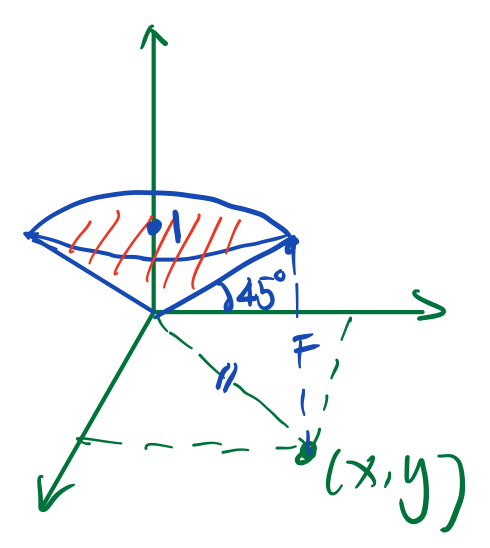
\includegraphics[scale=0.25]{images/Ch10-cone.jpeg}
    \end{center}
    {\bf Remark: }When one of the variables is missing from the equation, 
    the equation represents a surface {\it parallel} to the axis of the 
    missing variable.

    \eg $z=x^2$, since $y$ is missing, we draw a parabola and move it 
    along the $y$ axis.
    \begin{center}
        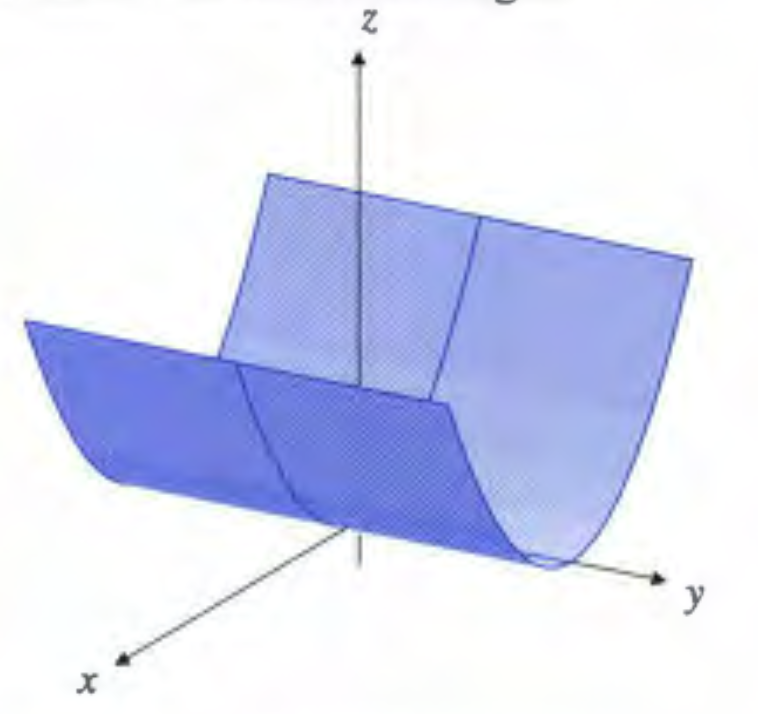
\includegraphics[scale=0.3]{images/Ch10-parabola-ymissing.png}
    \end{center}

    \section{Vectors}
    \subsection{Vectors and Properties}

    In $\mathbb{R}^3$, $\vct{r}=(a,b,c)=a\vct{i}+b\vct{j}+c\vct{k},\  
    ||\vct{r}||=\sqrt{a^2+b^2+c^2}$

    {\bf Zero vector} $\vct{0}$ has length zero and no specific direction.

    {\bf Properties of vectors}
    \begin{itemize}
        \item Equality: iff same {\bf magnitude }and same {\bf direction}.
        OR, their {\bf components} equal 
        \item Parallel: $\vct{r}=\lambda \vct{s}$
        \item Negative: $-\vct{r}$ has same magnitude but opposite direction.
        \item Addition, Subtraction, Scalar Multiplication: omit.
    \end{itemize}

    {\bf Unit Vector:} $\hat{\vct{r}}=\dfrac{\vct{r}}{||\vct{r}||}$

    {\bf Dot Product:} $\vct{u}\cdot \vct{v}=u_1v_1+u_2v_2+u_3v_3$.
    {\bf Remark: } $\vct{a}\cdot \vct{b}=\vct{a}\cdot \vct{c} \nRightarrow \vct{b}=\vct{c}$

    {\bf Angle:} $\vct{u}\cdot \vct{v}=||\vct{u}||\cdot ||\vct{v}||\cos\theta$

    {\bf Projections:}
    \begin{itemize}
        \item Scalar projection: $s=\dfrac{\vct{u}\cdot \vct{v}}{||\vct{v}||}=
        ||\vct{u}||\cos \theta$
        \item Vector projection of $\vct{u}$ in the direction of $\vct{v}$: 
        $\vct{u}_{\vct{v}}=\dfrac{\uu\cdot \vv}{||\vv||}\hat{\vv}=
        \dfrac{\uu\cdot \vv}{||\vv||^2}\vv$
    \end{itemize}

    \eg Find the scalar and vector projections of vector $\va=\ii-2\jj+\kk$ on
    the vector $\bb=4\ii-4\jj+7\kk$.

    \sol $$s=\frac{\va\cdot \bb}{||\bb||}=\frac{4+8+7}{\sqrt{4^2+4^2+7^2}}=\frac{19}{9}$$
    $$\va_{\bb}=s\cdot \frac{\bb}{||\bb||}=\frac{19}{81}(4\ii-4\jj+7\kk)$$

    {\bf Position Vector:} $\rr$ from the origin to the point $(a,b,c)$: 
    $$\rr = a\ii+b\jj+c\kk,\qquad ||\rr||=\sqrt{a^2+b^2+c^2}$$
    $$\hat{\rr}=\frac{a\ii+b\jj+c\kk}{\sqrt{a^2+B^2+c^2}}$$

    {\bf Cross Product:}
    \def\arraystretch{0.8}
    \begin{align*} 
        \uu \times \vv &=\left|
            \begin{array}{ccc}
                \ii & \jj & \kk \\ 
                u_{1} & u_{2} & u_{3} \\ 
                v_{1} & v_{2} & v_{3}
            \end{array}
            \right|
        =\left(u_{2} v_{3}-u_{3} v_{2}\right) \ii-
        \left(u_{1} v_{3}-u_{3} v_{1}\right) \jj+
        \left(u_{1} v_{2}-u_{2} v_{1}\right) \kk \\ 
        &=-\vv \times \uu \quad \text { \bf (vector) } 
    \end{align*}
    {\bf Properties:}
    \begin{itemize}
        \item $\uu\times \uu = \vct{0}$
        \item $\va\times(\bb+\cc)=\va\times \bb+\va\times \cc$
        \item $(\uu\times \vv)\cdot \uu=0, (\uu\times \vv)\cdot \vv=0$
        \item $||\uu\times \vv||=||\uu||\cdot ||\vv||\sin\theta=$ area of parallelogram.
        \begin{center}
            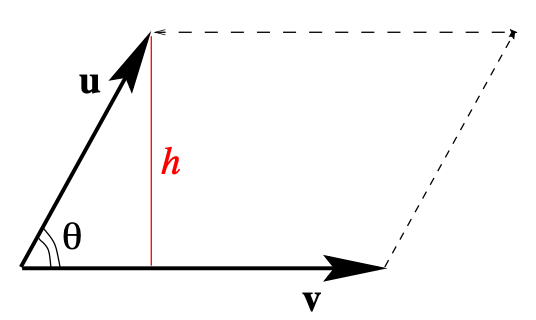
\includegraphics[scale=0.5]{images/Ch10-cross-product-geometry.png}
        \end{center}
        \item $||\uu \times \vv||^2=||\uu||^2||\vv||^2-(\uu\cdot \vv)^2$
        \item $\uu\times(\vv\times \ww)\ne (\uu\times \vv)\times \ww$
        \item $\vct{a}\times \vct{b}=\vct{a}\times \vct{c} \nRightarrow \vct{b}=\vct{c}$
    \end{itemize}

    \subsection{Triple Scalar Products}
    $$\va\cdot (\bb\times \cc)=a_{1}\left|
    \begin{array}
        {ll}b_{2} & b_{3} \\ 
        c_{2} & c_{3}
    \end{array}\right|-
    a_{2}\left|
    \begin{array}{ll}
        b_{1} & b_{3} \\ 
        c_{1} & c_{3}
    \end{array}\right|+
    a_{3}\left|
    \begin{array}{ll}
        b_{1} & b_{2} \\ 
        c_{1} & c_{2}
    \end{array}\right|=
    \left|
    \begin{array}{lll}
        a_{1} & a_{2} & a_{3} \\ 
        b_{1} & b_{2} & b_{3} \\ 
        c_{1} & c_{2} & c_{3}
    \end{array}\right|$$
    
    {\bf Geometric interpretation} of $\va\cdot (\bb\times \cc)$: 
    \begin{align*}
        \va\cdot (\bb\times \cc) &= ||\va||\ ||\bb\times \cc||\cos\theta \\
        &= \left(||\va||\cos\theta\right)\cdot ||\bb\times \cc||\\
        &= h\cdot ||\bb\times \cc||\\
        &= \textbf{volume of the parallelepiped}
    \end{align*}
    \begin{center}
        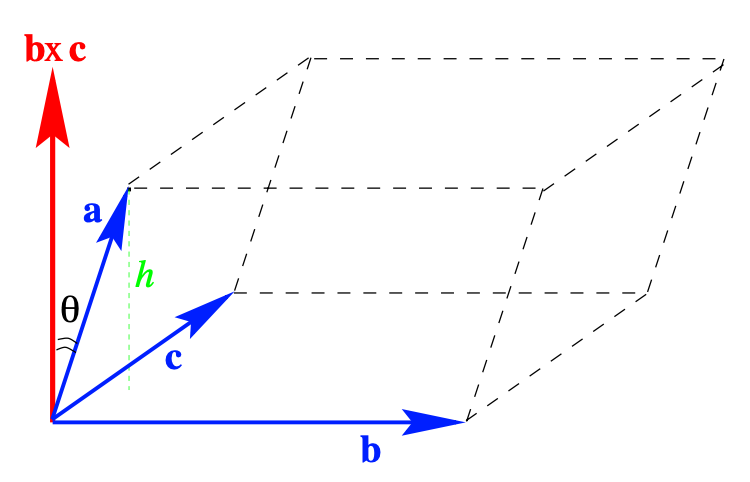
\includegraphics[scale=0.5]{images/Ch10-triple-scalar-prod.png}
    \end{center}

    Another use of triple scalar product is for deciding whether three 
    vectors are {\bf in the same plane}. If so, then $$(\va\times \bb)\cdot \cc=0$$

    \subsection{Triple Vector Products}

    $(\va\times \bb)\times \cc$ is in the plain containing $\va$ and $\bb$.
    \begin{center}
        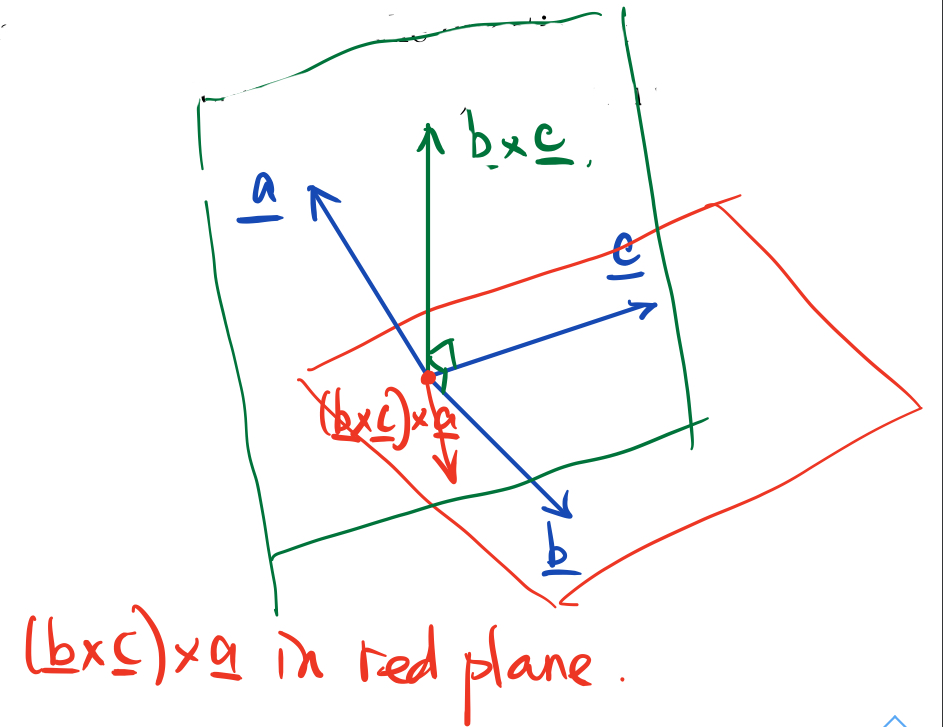
\includegraphics[scale=0.25]{images/Ch10-triple-cross-prod.jpeg}
    \end{center}

    \eg Construct three mutually orthogonal vectors in space, making use of 
    two non-parallel vectors $\va$ and $\bb$.

    \sol $\va$, $\va\times \bb$, and $\va\times(\va\times \bb)$.
    \begin{center}
        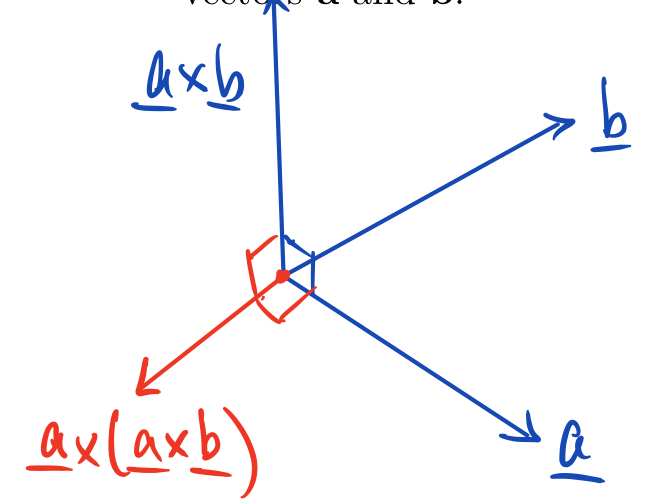
\includegraphics[scale=0.27]{images/Ch10-mutually-orth.jpeg}
    \end{center}

    \section{Planes and Lines}

    \subsection{Planes}

    {\bf The equation of a plane}: assume nonzero normal vector 
    $\vct{n}=A\ii+B\jj+C\kk$ and plane passes through $r_0=(x_0,y_0,z_0)$,
    $$\vct{n}\cdot (\vct{r}-\vct{r_0})=0$$
    can also written in {\bf standard form}: 
    $$Ax+By+Cz=Ax_0+By_0+Cz_0$$

    {\bf A pencil of planes}: a family of plans intersecting in a straight line.
    If two nonparallel planes have equations $A_1x+B_1y+C_1z=D1$ and 
    $A_2x+B_2y+C_2z=D_2$, then 
    $$A_1x+B_1y+C_1z-D1+\lambda(A_2x+B_2y+C_2z-D_2)=0$$
    represents a plane in the pencil, where $\lambda\in \mathbb{R}$.
    \begin{center}
        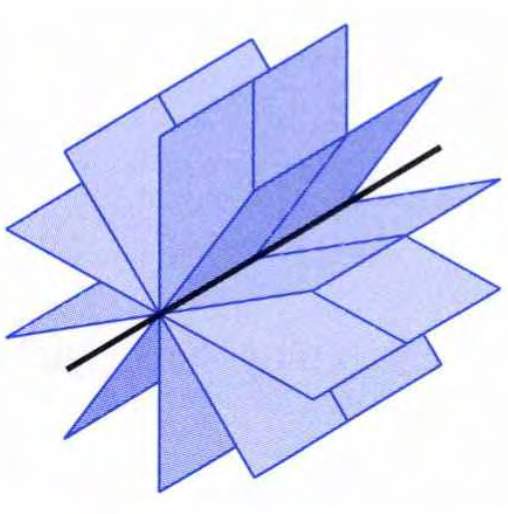
\includegraphics[scale=0.4]{images/Ch10-pencils-of-planes.png}
    \end{center}

    \eg Find the equation of the plane through $P_0=(-1,4,2)$ and 
    containing the line of intersection of the planes 
    $4x-y+z-2=0$ and $2x+y-2z-3=0$.

    \sol Two methods: 

    {\bf (1) find three points.} 

    Notice the two planes have infinity points intersected. 
    We arbitrarily choose 2 of them, say 
    $\vct{r_1}=(0,-7,-5), \vct{r_2}=(1,3,1)$. Another point is given in problem,
    $\vct{r_0}=(-1,4,2)$.

    Then a normal vector can be 
    $(\vct{r_1}-\vct{r_0})\times (\vct{r_2}-\vct{r_0})=(4,-13,21)$

    {\bf (2) find the pencil of planes.}

    The pencil of planes formed by the given two non-parallel planes is 
    $$4x-y+z-2+\lambda(2x+y-2z-3)=0$$
    Since the plane is inside the pencil and containing $P_0$,
    substitute $(-1,4,2)$ into the equation, we get $\lambda=-\dfrac{8}{5}.$

    \subsection{Lines}

    {\bf Vector parametric equation of straight line:} with a point 
    $\vct{r_0}$ and {\bf direction vector }$\vv$: 
    $$\vct{r}(t)=\vct{r_0}+t\vv$$

    \eg Find the vector equation for the line segment joins $P_1=(2,4,-1)$
    and $P_2=(5,0,7)$.

    \sol direction vector $\vv=(3,-4,8)$, thus 
    $$\vct{r}(t)=(2,4,-1)+t\cdot (3,-4,8),\ \red{0\le t\le 1}$$

    \eg Find the intersection of line $\vct{r}=\vct{r_0}+t\vct{v}$ 
    and plane $\vct{r}\cdot \vv=d$, assume they are not parallel.

    \sol $(\vct{r_0}+t\vv)\cdot \vct{n}=d$, solve for $t$.

    \subsection{Distances}

    {\bf Point to Line:} 

    \begin{center}
        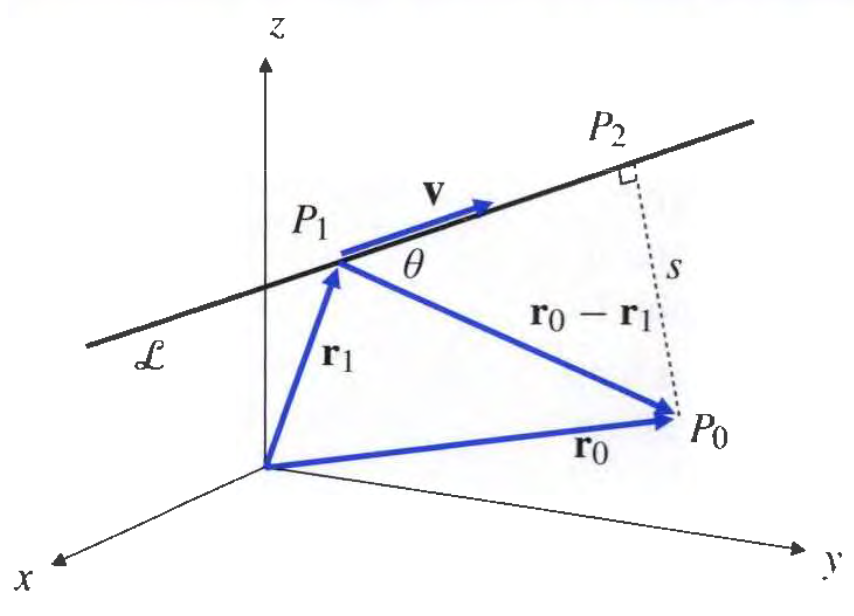
\includegraphics[scale=0.4]{images/Ch10-dist-point-line.png}
    \end{center}
    \begin{align*}
        d &= ||\vct{r_1}-\vct{r_0}||\cdot \sin\theta \cdot 1\\
         &= ||\vct{r_1}-\vct{r_0}||\cdot \sin\theta \cdot ||\hat{\vv}||\\
         &= ||(\vct{r_1}-\vct{r_0})\times \hat{\vv}||
    \end{align*}

    {\bf Point to Plane:} 
    \begin{align*}
        d &= ||\vct{r_1}-\vct{r_0}||\cdot \cos\theta \cdot 1\\
         &= ||\vct{r_1}-\vct{r_0}||\cdot \cos\theta \cdot ||\hat{\vct{n}}||\\
         &= | (\vct{r_1}-\vct{r_0})\cdot \hat{\vct{n}} |
    \end{align*}
    \begin{center}
        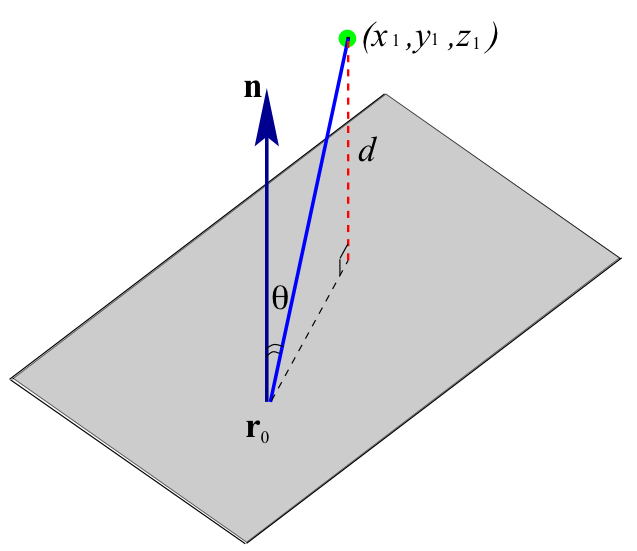
\includegraphics[scale=0.3]{images/Ch10-dist-point-plane-2.jpeg}
    \end{center}


    {\bf Line to Plane(parallel): } Take any point on the line $\rar$ point to plane.

    {\bf Parallel Lines: } Same as point to line.

    {\bf Skew Lines:} 

    \begin{center}
        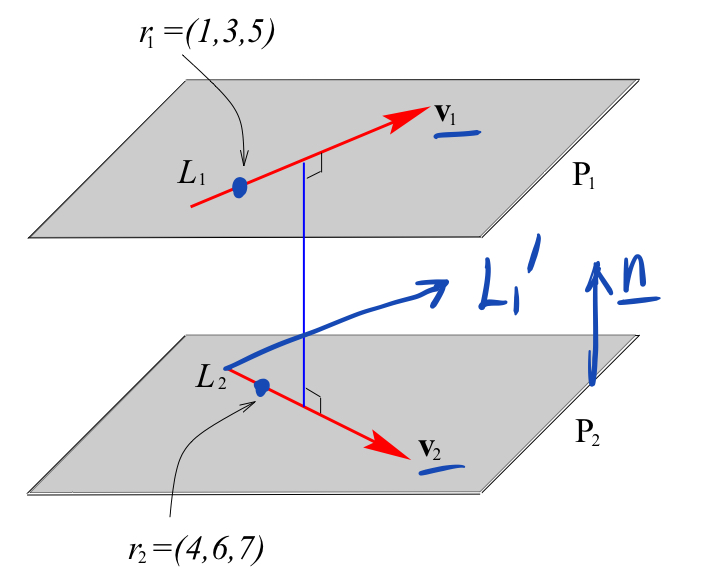
\includegraphics[scale=0.3]{images/Ch10-dist-line-line.jpeg}
    \end{center}

    Make $L_1$ and $L_1$ inside the same plane, then normal vector of 
    the plane is $\vct{n}=\vct{v_1}\times \vct{v_2}$.

    Now it is the same as line to plane.
    \begin{align*}
        d &= | (\vct{r_1}-\vct{r_0})\cdot \hat{\vct{n}} |\\
         &= | (\vct{r_1}-\vct{r_0})\cdot \widehat{(\vct{v_1}\times \vct{v_2})} |
    \end{align*}

    
    {\bf Plane to Plane(parallel):} same as point to plane. 


    \section{Quadric Surfaces}


    {\bf Spheres}: $(x-x_0)^2+(y-y_0)^2+(z-z_0)^2=a^2$.

    {\bf Cylinders:} $x^2+y^2=a^2$. (left below)

    {\bf Cones:} $z^2=x^2+y^2$. (right below)
    
    \begin{center}
        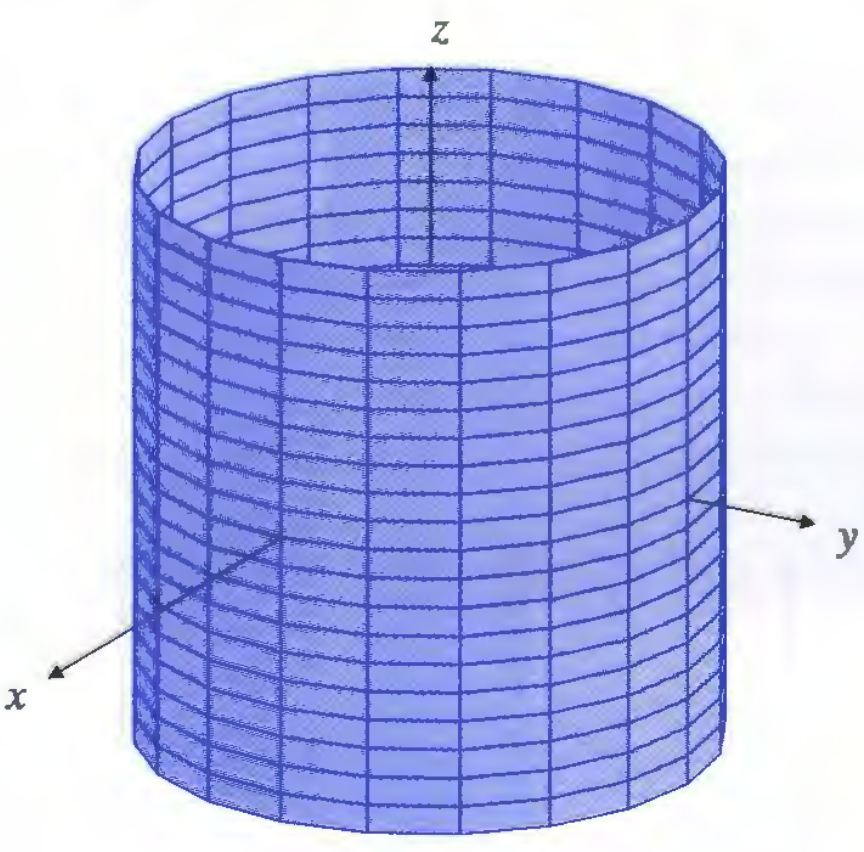
\includegraphics[scale=0.3]{images/Ch10-cylinder.png}
        \hspace{1in}
        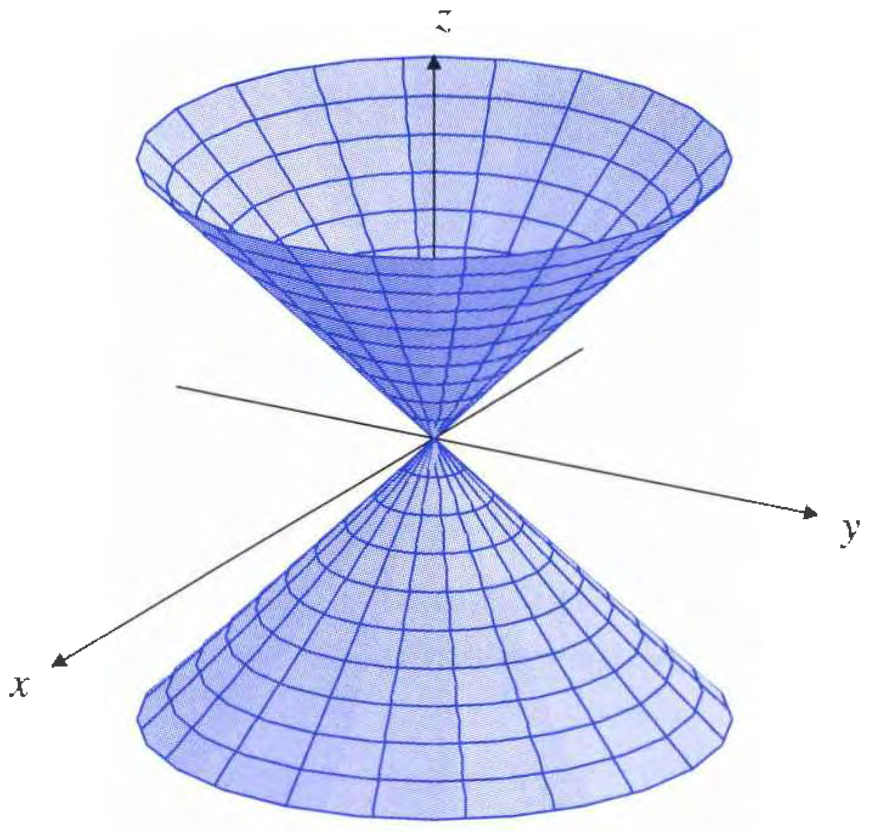
\includegraphics[scale=0.3]{images/Ch10-cone.png}
    \end{center}
    

    {\bf Ellipsoid:} $\disp \frac{x^2}{a^2}+\frac{y^2}{b^2}+\frac{z^2}{c^2}=1$. (left below)

    {\bf Elliptic paraboloid:} $\disp z=\frac{x^2}{a^2}+\frac{y^2}{b^2}$. (right below)

    \begin{center}
        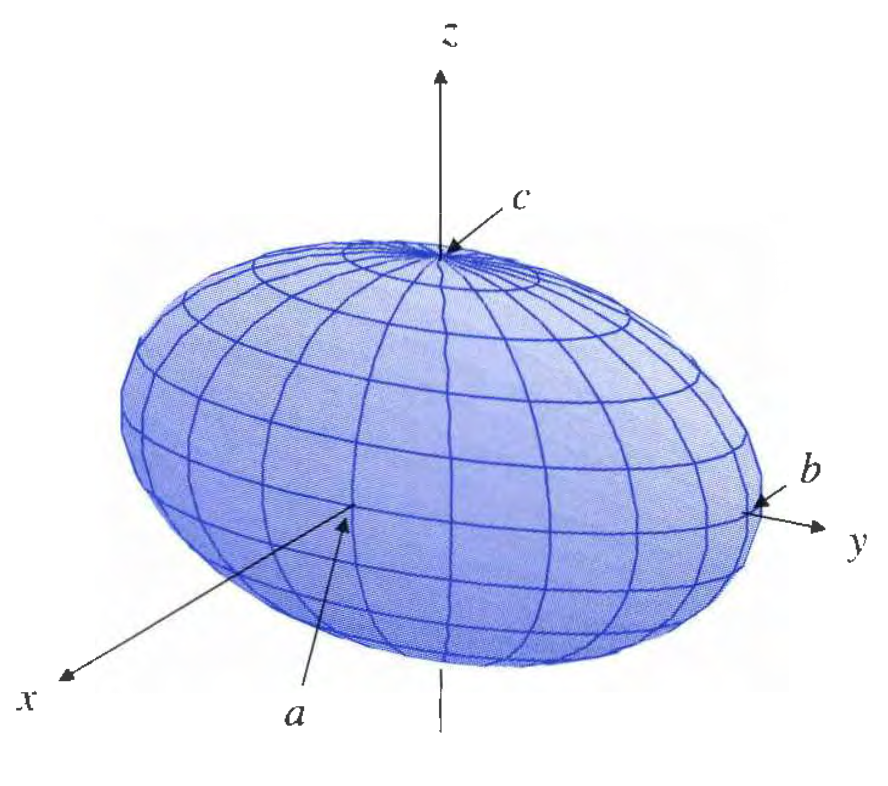
\includegraphics[scale=0.3]{images/Ch10-ellipsoid.png}
        \hspace{1in}
        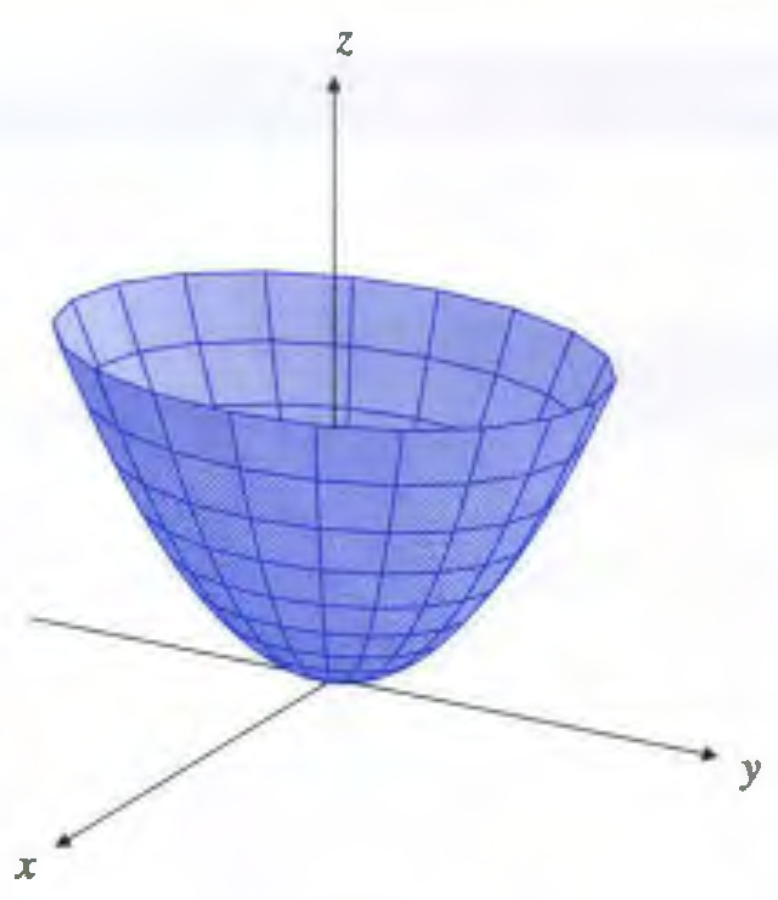
\includegraphics[scale=0.3]{images/Ch10-elliptic-paraboloid.png}
    \end{center}

    {\bf Hyperbolic paraboloid :} $\disp z=\frac{x^2}{a^2}-\frac{y^2}{b^2}$.

    \begin{center}
        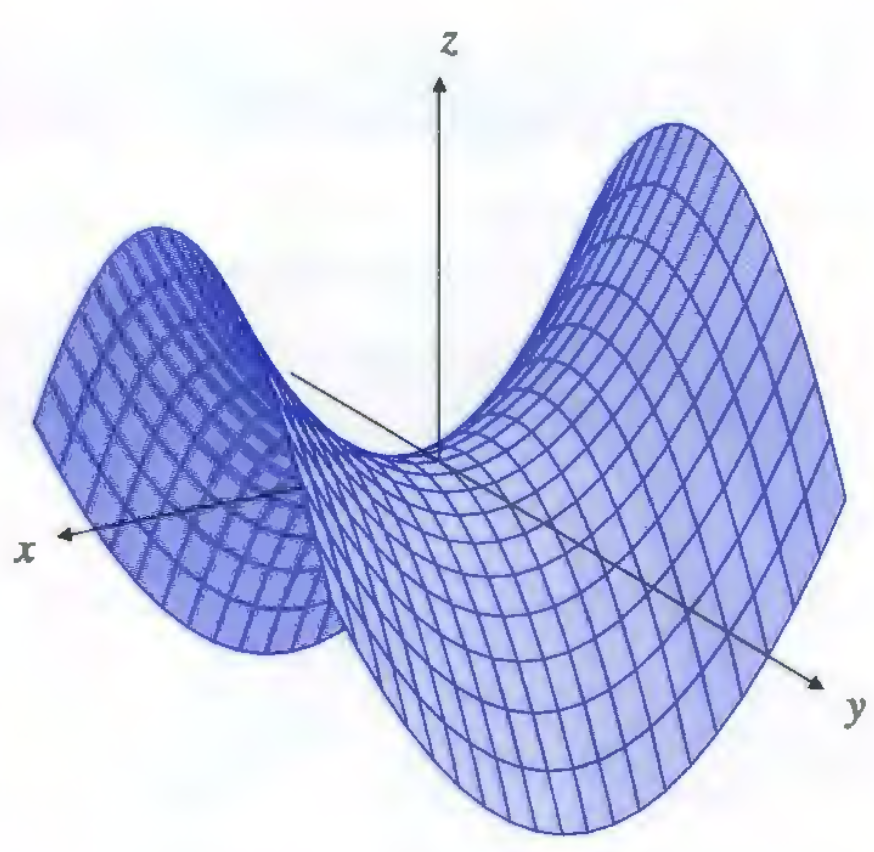
\includegraphics[scale=0.3]{images/Ch10-hyperbolic-paraboloid.png}
    \end{center}

    {\bf Hyperboloids:}
    \begin{center}
        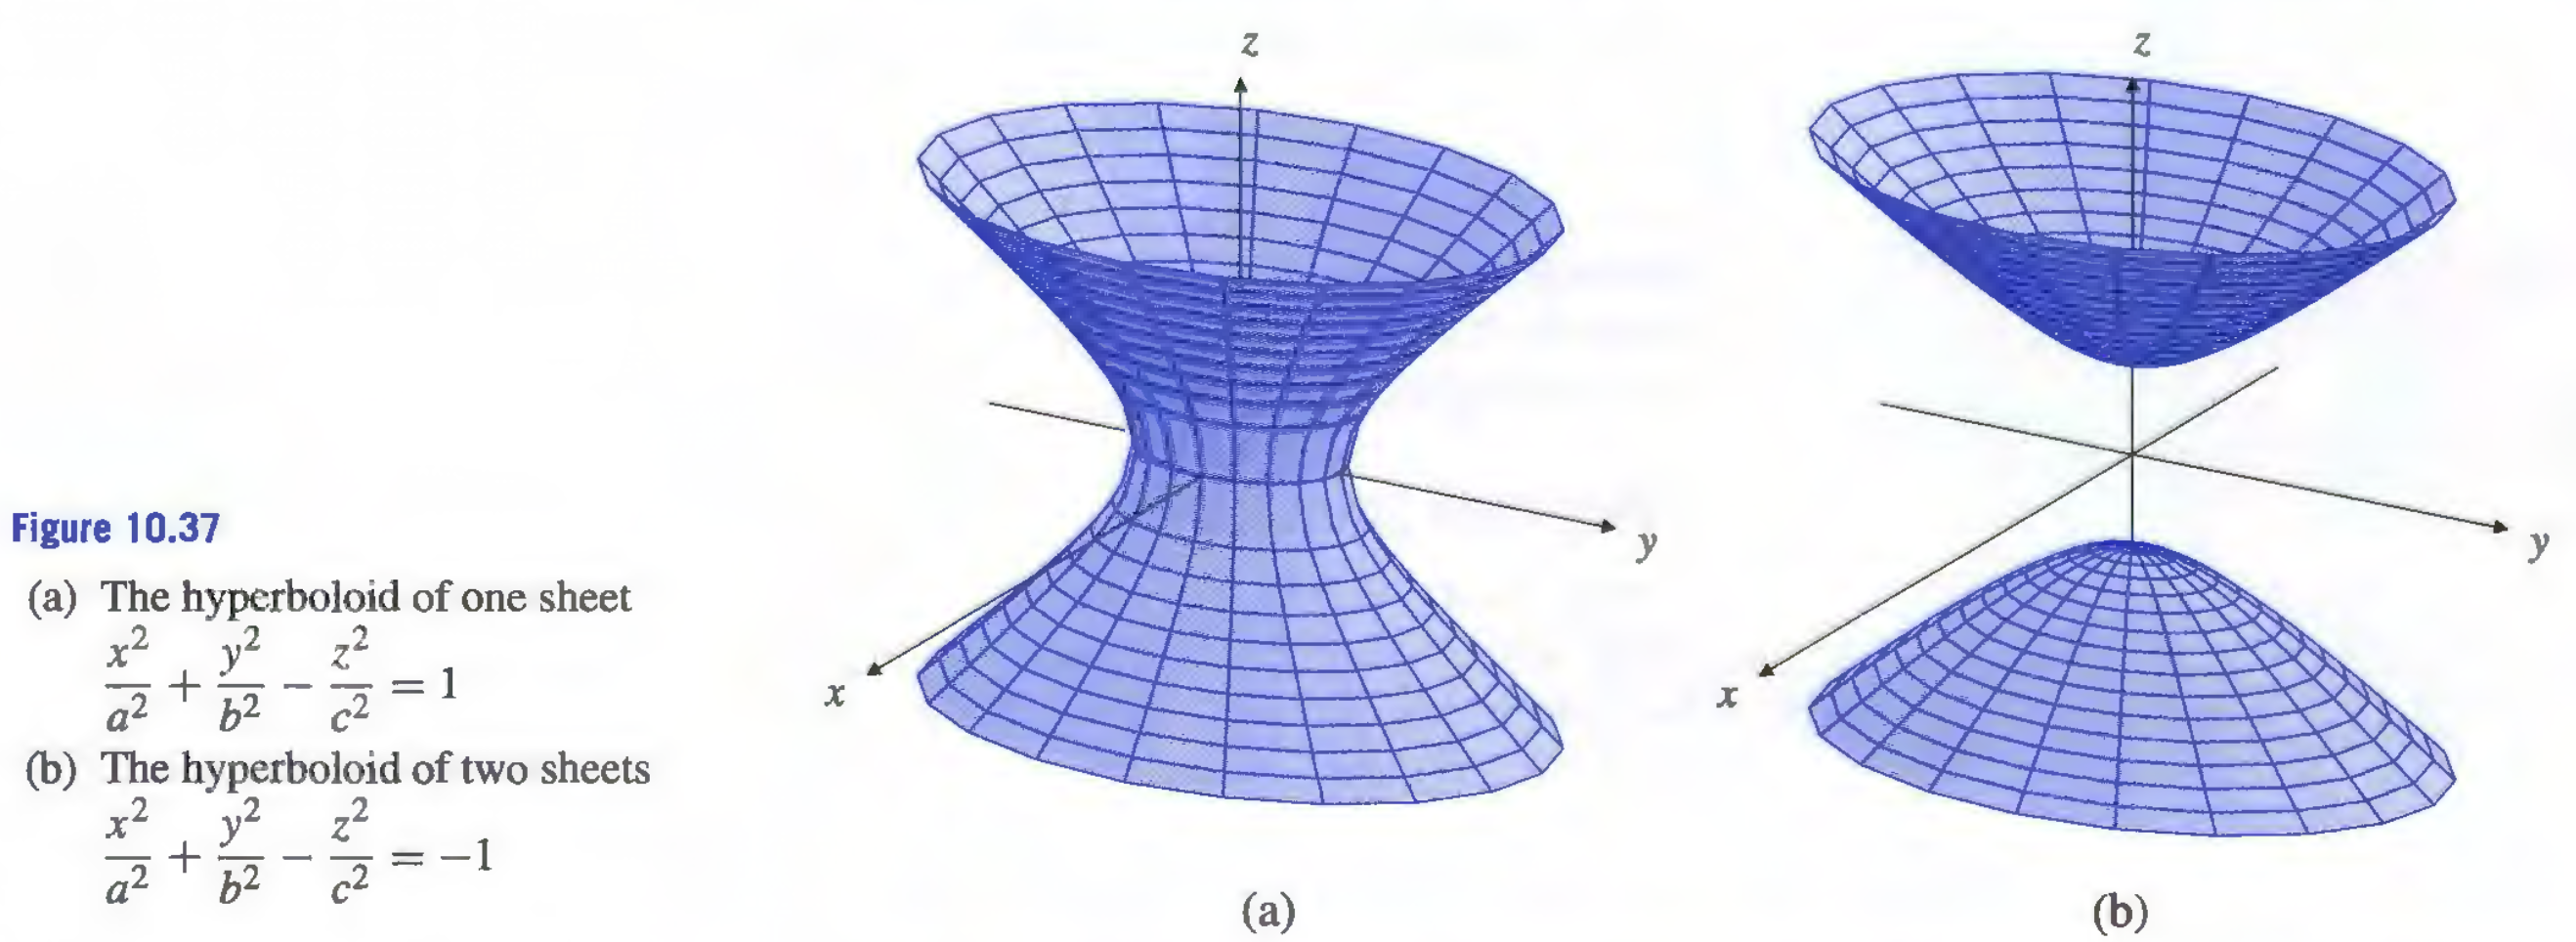
\includegraphics[scale=0.37]{images/Ch10-hyperboloid.png}
    \end{center}

    \section{Cylindrical and Spherical Coordinates}

    {\bf Cylindrical Coordinate:} $(r,\theta,z)$
    \begin{align*}
        x &= r\cos\theta\\ y&=r\sin\theta\\z&=z
    \end{align*}
    where $r\ge 0,\ 0\le \theta<2\pi$, and 
    \begin{align*}
        r &= \sqrt{x^2+y^2}\\
        \theta &= \left\{ \begin{array}{ll}
            \tan^{-1}(y/x) & {\rm if}\ x\ge 0\\
            \tan^{-1}(y/x)+\pi & {\rm if}\ x<0
        \end{array}\right.
    \end{align*}

    \begin{center}
        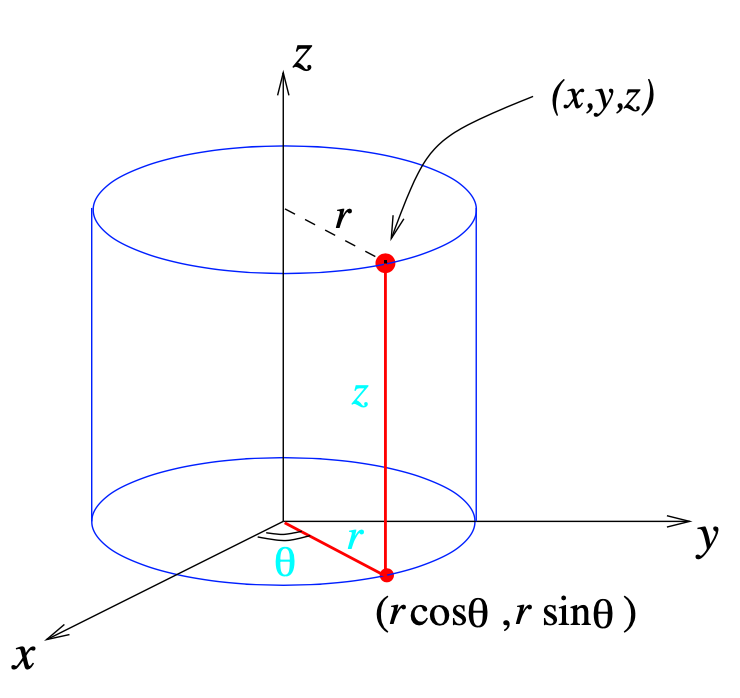
\includegraphics[scale=0.4]{images/Ch10-cylindrical-coor.png}
        \hspace{1in}
        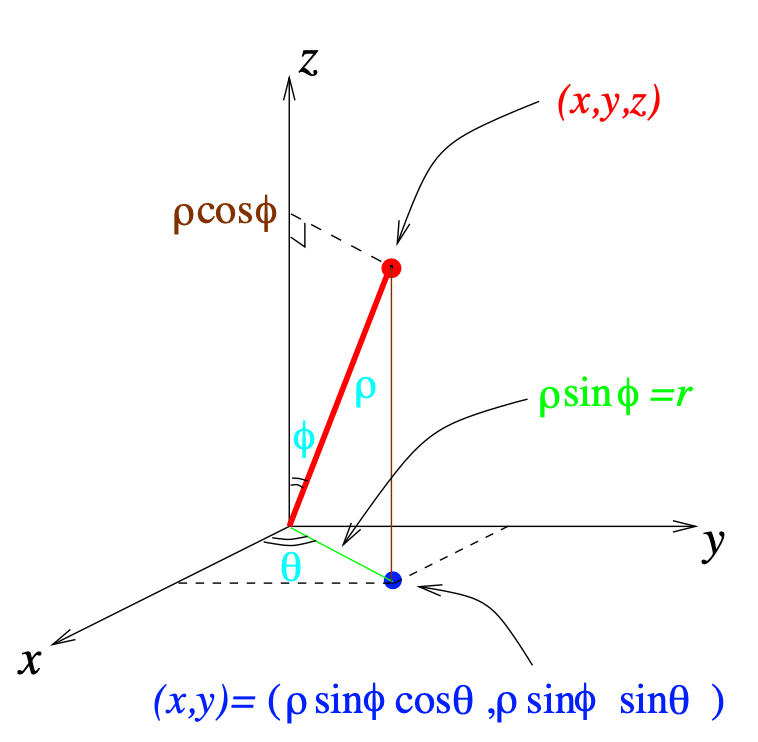
\includegraphics[scale=0.4]{images/Ch10-spherical-coor.png}
    \end{center}

    {\bf Spherical Coordinates: } $(\rho, \theta,\phi)$
    \begin{align*}
        x &= r\cos\theta=\rho\sin\phi\cos\theta\\
        y &= r\sin\theta=\rho\sin\phi\sin\theta\\
        z &= \rho\cos\phi
    \end{align*}
    where $\rho\ge 0,\ 0\le \theta<2\pi,\ 0\le \phi\le \pi$, and 
    \begin{align*}
        \rho &= \sqrt{x^2+y^2+z^2}\\
        \theta &= \left\{ \begin{array}{ll}
            \tan^{-1}(y/x) & {\rm if}\ x\ge 0\\
            \tan^{-1}(y/x)+\pi & {\rm if}\ x<0
        \end{array}\right.\\
        \phi &= \cos^{-1}(z/\rho)
    \end{align*}
\end{spacing}


\chapter{Chapter 11: Vector Functions and Curves}

% 
\begin{spacing}{1.3}
    
    \section{Intro: Binary Search}

    The main idea of {\rm Divide \& Conquer} is to solve a problem(such as of 
    size $n$) by breaking it into one or more smaller(size less than $n$) problems.
    We use binary search example to illustrate that.

    {\bf Problem:} given an {\bf sorted} array of length $n$, how to find 
    the position of element $x$; if $x$ does not exist
    in the array, output nil.

    Since the array is already sorted, it has a good property that:
    {\bf for each item $a_i$, those who are larger than $a_i$ must be 
    on its right side, while smaller than $a_i$ must be on its left side.}
    Hence we come up with an idea that we check the middle item $mid$ first,
    then we will be able to know which direction to go: left or right,
    depending on the comparison of $mid$ and $x$(the item we're looking for).
    If we go left, then the right half will be directly abandoned.
    Then we continue this process, check middle item each time, and 
    abandon half items each time.

    \newpage
    \begin{algorithm}[H]
        \setstretch{1.1}
        \caption{BinarySearch($a[]$, $left$, $right$, $x$)}
        \KwData{$a[]$: the array given, $x$: the item to find}
        \eIf{$left=right$}{
            \eIf{$a[left]=x$}{
                return $left$
            }{
                return {\bf nil}
            }
        }{
            $mid=\lfloor (left + right) / 2\rfloor$

            \eIf{$x\le a[mid]$} {
                BinarySearch($a[]$, $left$, $mid$, $x$)
            }{
                BinarySearch($a[]$, $mid+1$, $right$, $x$)
            }
        }
    \end{algorithm}

    {\bf First call:} BinarySearch($a[]$, 1, $n$, $x$).

    This algorithm is quite efficient, since each time 
    we eliminate half of the array, with one additional 
    comparison, until there is only one item left,
    when we will end the process.

    Then let's analyse its time complexity. Let $T(n)$ be the number of 
    comparisons needed for $n$ elements, then we will have
    $$T(n)=T(n/2)+1,\ T(1)=1$$.

    Solve this {\bf recurrence}:
    \begin{align*}
        T(n) &= T(n/2) + 1\\
            &= [T(n/4) + 1] + 1\\
            &= T(n/4) + 2\\
            &=\cdots\\
            &=T(n/2^{i}) + i
    \end{align*}

    This process ends when reaching $T(1)$, i.e., 
    $i=\log_2 n$, thus, $T(n)=T(1)+\log_2 n=\log_2 n + 1$.

    We can also visualize this recurrence with recursion tree:
    (image from lecture note)
    \begin{center}
        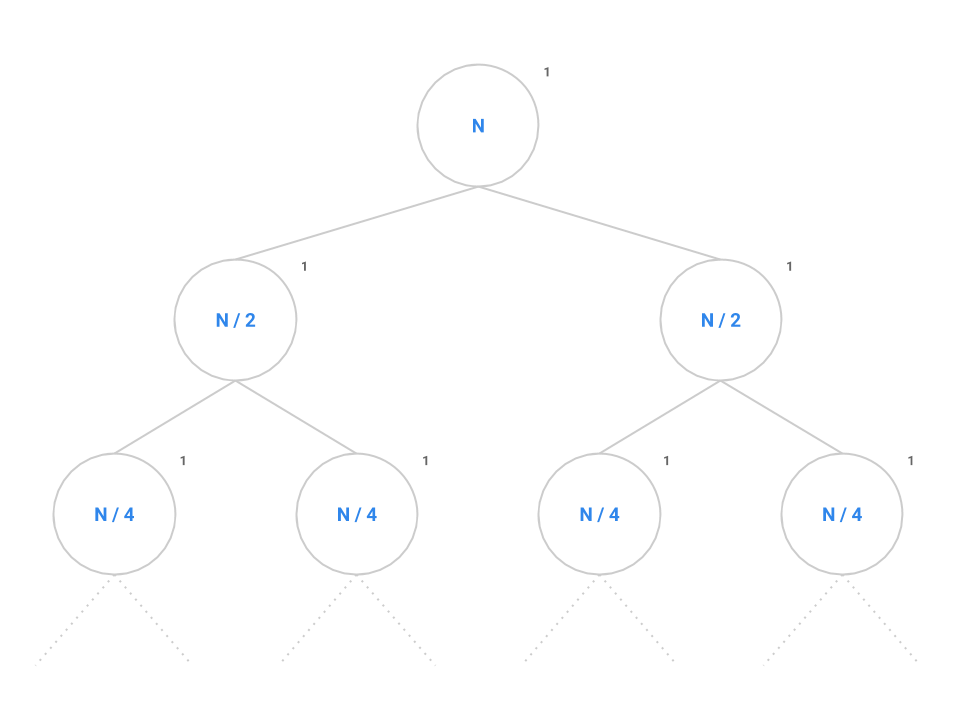
\includegraphics[scale=0.42]{images/02-bs-tree.png}
    \end{center}

    In each recursion step(level), we use 1 comparison(compare 
    $mid$ and $x$), then call recursion on a half 
    of the original array. From the image above, 
    we can easily notice there are total 
    $1+1+\cdots+1=1+\log_2 n$ comparisons.

    \newpage
    \section{Example: Towers of Hanoi}

    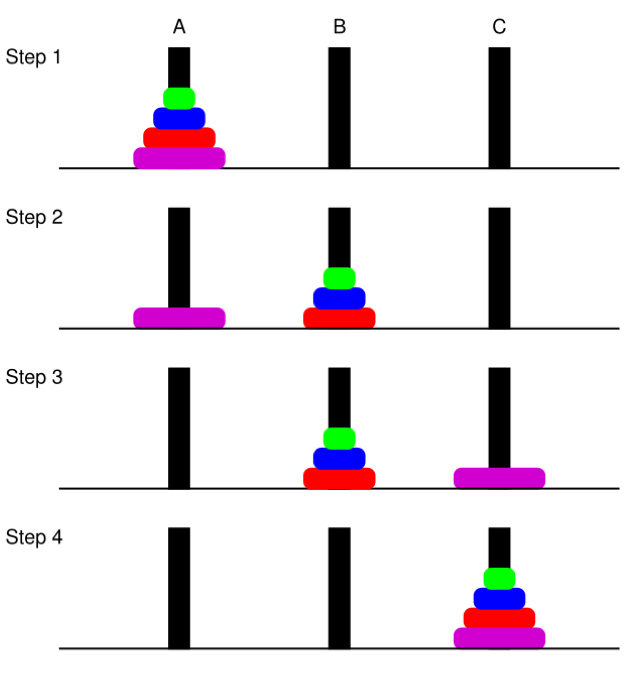
\includegraphics[scale=0.28]{images/02-hanoi.jpeg}
    
    In this example, we want to design an algorithm to 
    move all $n$ discs from peg $A$(start) to peg $C$(end), with the 
    constraints: (1) move one disc at a time, and 
    (2) cannot put larger disc on a smaller one.
    We are given another peg $B$(helper) where we can 
    temporary storage our discs.

    We still use the idea of {\bf Divide \& Conquer},
    consider how we can turn a problem of $n$ discs 
    into a problem of $n-1$? One possible solution is that,
    we can call recursion on upper $n-1$ discs, i.e., 
    move upper $n-1$ discs to peg $B$(helper peg), then move the remaining
    (the biggest) disc to peg $C$(end peg), and finally 
    move the $n-1$ discs from peg $B$(helper) to peg $C$(end).
    The following pseudocode shows this idea.

    \begin{algorithm}[H]
        \setstretch{1.1}
        \caption{MoveTower($n$, $start$, $helper$, $end$)}
        \KwIn{$n$: num of discs}
        \eIf{$n=1$}{
            move the only disc from $start$ peg to $end$ peg

            return
        }{
            {\tcp {move first $n-1$ from $start$ peg to $helper$ peg}}
            {\tcp {so this time ``helper'' peg will be the old $end$ peg}}
            {\bf MoveTower($n-1$, $start$, $end$, $helper$)}

            move the only disc from $start$ peg to $end$ peg

            {\tcp {finally move first $n-1$ from $helper$ peg to $end$ peg}}
            {\tcp {this time ``helper'' peg will be the old $start$ peg}}
            {\bf MoveTower($n-1$, $helper$, $start$, $end$)}
        }
    \end{algorithm}

    Now we would like to analyze the time complexity of this algorithm,
    in other words, how many {\bf steps} are needed.
    Let $T(n)$ be the num of steps for $n$ discs, each time, 
    we first move $n-1$ disks from $start$ to $helper$, 
    costs $T(n-1)$ steps; then we move the biggest disk to $end$ peg,
    costs only 1 step; finally we move $n-1$ disks from $helper$
    to $end$, again costs $T(n-1)$ steps. To sum up:
    $$T(n)=2T(n-1)+1$$ when $n>1$, and $T(1)=1$.

    Now we solve the recurrence by the {\bf expansion method}:
    \begin{align*}
        T(n) &= 2T(n-1) + 1\\
             &= 2[2T(n-2)+1] + 1\\
             &= 4T(n-2)+3\\
             &= 4[2T(n-3)+1] + 3 \\
             &= 8T(n-3) + 7\\
             &= \cdots \\
             &= 2^i T(n-i) + (2^i-1)\\
             &= 2^{n-1} T(1) + (2^{n-1}-1)\\
             &= 2^n-1
    \end{align*}

    Or, with the recursion tree method:
    \begin{center}
        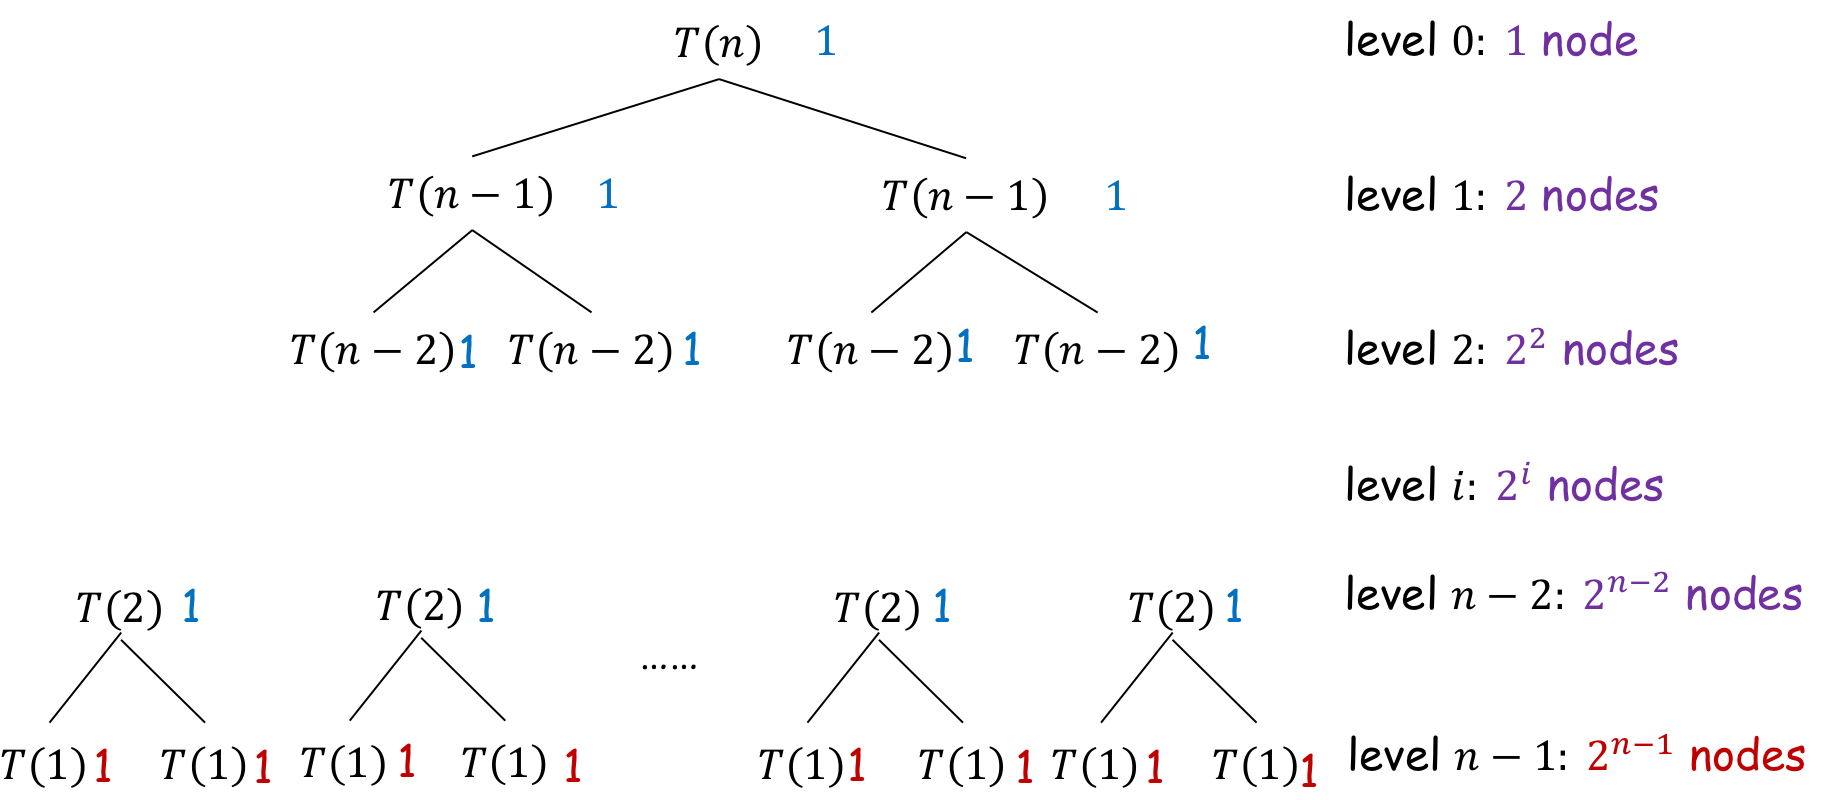
\includegraphics[scale=0.2]{images/02-hanoi-tree.jpeg}
    \end{center}
    
    There are, altogether, $1+2+2^2+2^3+\cdots + 2^{n-2}+2^{n-1}
    =2^n-1$ nodes, and we are doing one work(step) each node,
    then the time complexity is again, $2^n-1$.

    \newpage
    \section{Merge Sort}

    Now we again back to sorting, and we would like to introduce 
    a new algorithm or sorting: Merge Sort.
    This is a typical example of divide \& conquer, and 
    its process is like: (1) we first divide array into two halves,
    (2) then we recursively sort each half, (which means we 
    continuously divide it into halves, and then halves...)
    (3) finally {\bf merge} two halves to get a whole.

    The {\bf merge} operation may confuse you most. Here 
    it means combine two {\bf sorted lists} into a 
    whole sorted list. For example, given two sorted lists:
    $A=[2, 5, 7]$ and $B=[3, 4, 6, 10, 12]$, then after {\bf merge}
    operation, we will get $result=[2, 3, 4, 5, 6, 7, 10, 12]$.
    Since these two lists are sorted, we can do this process
    in $O(n)$ time, where $n$ is the length of result 
    list.(how many numbers in total) The basic idea is: 
    we compare the first item of $A$ and $B$, put the smaller 
    one, say, $A[1]$, in the first position of result list, then 
    we move on to the next item of $A$, but compare it still with 
    the {\bf first} item of $B$(since the first item of $B$
    has not yet inserted into result list), 
    and again put the smaller one into result list, then 
    continue move on. An example may help you understand the process:

    \noindent (1) Compare first items: $A=[{\blue 2},5,7], B=[{\blue 3},4,6,10,12]$, 
    $2<3$, so $result=[2]$;\\
    (2) then compare 2nd in $A$ and 1st in $B$, $A=[2, {\blue 5},7], B=[{\blue 3},4,6,10,12]$, 
    $3<5$, so $result=[2, 3]$;\\
    (3) continue the process, similarly, $A=[2, {\blue 5},7], B=[3,{\blue 4},6,10,12]$, 
    $4<5$, so $result=[2, 3, 4]$;\\
    (4) $A=[2, {\blue 5},7], B=[3,4,{\blue 6},10,12]$, 
    $5<6$, so $result=[2, 3, 4, 5]$;\\
    (5) $A=[2, 5,{\blue 7}], B=[3,4,{\blue 6},10,12]$, 
    $6<7$, so $result=[2, 3, 4, 5, 6]$;\\
    (6) $A=[2, 5,{\blue 7}], B=[3,4,6,{\blue 10},12]$, 
    $7<10$, so $result=[2, 3, 4, 5, 6, 7]$;\\
    (7) Now, all items in $A$ have already been inserted into result 
    list so that no items can be compared with items in $B$.
    Then we simply add remaining items in $B$ to result list,
    this will, obviously, ensure a sorted result list.(you may think of why)
    Hence $result=[2,3,4,5,6,7,{\blue 10,12}]$

    The pseudocode below shows the process:
    (below, append $\infty$ at the end of two lists can 
    free us from considering the situation that one list is 
    empty, like (7) above. Though different implementation, 
    the idea is entirely the same)
    
    \newpage
    \begin{algorithm}[H]
        \setstretch{1.1}
        \caption{Merge($A$, $left$, $mid$, $right$)}
        \tcp{merge two sorted list: $A[left\cdots mid]$ and $A[mid+1\cdots right]$}
        $L\lar A[left\cdots mid],\ R\lar A[mid+1\cdots right]$

        append $\infty$ at the end of $L$ and $R$ \qquad \tcp{see explanation above}

        $i\lar 1,\ j\lar 1$\qquad  \tcp{two pointers point at items in $L$ and $R$}

        \For{$k\lar left$ {\rm to} $right$} {
            \tcp{always choose the smaller one to insert, and move on}
            \eIf{$L[i] \le R[j]$}{
                $A[k]\lar L[i]$

                $i\lar i + 1$
            }{
                $A[k] \lar R[j]$

                $j\lar j + 1$
            }
        }
    \end{algorithm}

    After learning how {\bf Merge} works, you now, hopefully,
    are able to understand how Merge Sort works, with the image below:

    \begin{center}
        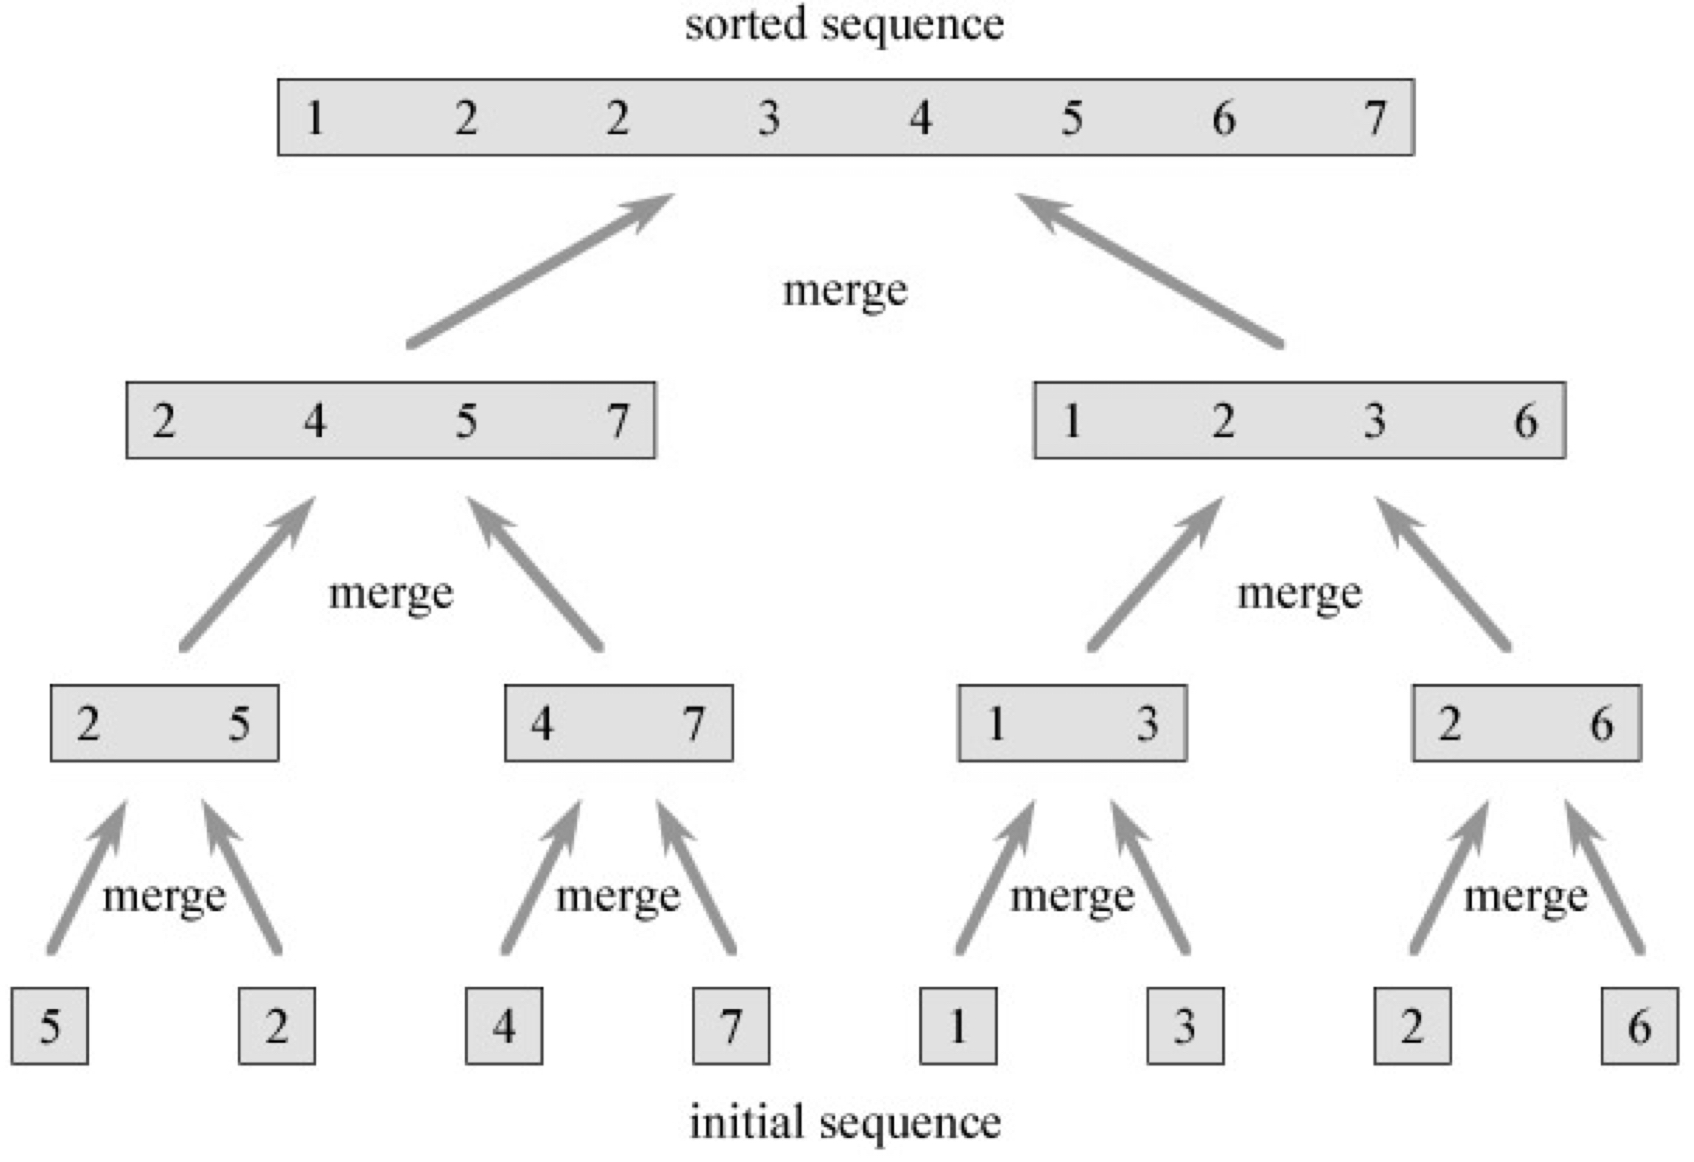
\includegraphics[scale=0.17]{images/02-mergeSort.jpeg}
    \end{center}
    
    We break down array recursively, until one element left,
    and then merge from bottom to up.
    The complete pseudocode for Merge Sort is given below:

    \newpage
    \begin{algorithm}[H]
        \setstretch{1.1}
        \caption{MergeSort($A$, $left$, $right$)}
        \If{$left=right$}{return}
        $mid\lar \lfloor (left + right) / 2 \rfloor$

        \tcp{recursively divide array into two halves}

        {\bf MergeSort($A$, $left$, $mid$)}

        {\bf MergeSort($A$, $mid+1$, $right$)}

        \tcp{then merge from bottom to up}

        {\bf Merge($A$, $left$, $mid$, $right$)}
    \end{algorithm}

    Firstly call {\bf MergeSort($A$, 1, $n$)} to sort array $A$.
    
    As usual, we are interested in the running time of Merge Sort 
    algorithm. Let $T(n)$ be the running time on an array of size $n$,
    it's not hard to find 
    $T(n)\le T(\lfloor n/2 \rfloor) + T(\lceil n/2 \rceil)+O(n)$,
    when $n>1$ and $T(1)=O(1)$.

    Here we are actually able to simplify the equation. Firstly 
    we can replace $\le $ with $=$, since we are interested
    in big-$O$ upper bound of $T(n)$; and with the same 
    reason, we can replace $O(n)$ with $n$, $O(1)$ with 1;
    finally, we can assume $n$ is a power of 2 for the sake of 
    simplicity but doesn't change the result at all, as 
    $T(n)\le T(n')\le T(2n)=O(T(n))$ where $n'$ is the 
    smallest power of 2 such that $n'\ge n$.

    Now we want to solve: 
    $T(n)=2T(n/2)+n$ for $n>1$, and $T(1)=1$.
    \begin{align*}
        T(n) &= 2\left(\frac{n}{2}\right)+n\\
             &= 2\left[ 2T\left(\frac{n}{4}\right) +\frac{n}{2}\right] + n
              = 2^2\cdot T\left(\frac{n}{2^2}\right) +2n\\
             &= 2^2\cdot \left[ 2T\left(\frac{n}{2^3}\right) +\frac{n}{2^2}\right] + 2n
              = 2^3\cdot T\left(\frac{n}{2^3}\right) +3n\\
             &= \cdots\\
             &= 2^{k}\cdot T\left(\frac{n}{2^k}\right) +kn
    \end{align*}
    We know the process ends with $\dfrac{n}{2^k}=1$ i.e. $k=\log_2 n$, thus
    \begin{align*}
        T(n) &= 2^{\log_2 n}T\left(\frac{n}{2^{\log_2 n}}\right)+n\cdot \log_2 n\\
             &= n\log_2 n+n
    \end{align*}
    In summary, merge sort runs in $O(n\log n)$ time.
    It is also worth pointing out that merge sort {\bf always}
    runs in $O(n\log n)$ time, which means best case is the same 
    as worst case, as you may think of it, 
    the complexity of merge sort {\it does not depend on inputs},
    it always break array down and then merge up.

    \newpage
    \section{Inversion Numbers}

    Given an array $A[1\cdots n]$, we say two elements $A[i]$ and $A[j]$
    are {\bf inverted} if $i<j$ but $A[i]>A[j]$, i.e., $A[i]$ appears
    before $A[j]$ but is larger than $A[j]$. The number of inverted pairs
    is called the {\bf inversion number} of array $A$. 
    Actually this is a useful measure, it provides us with an intuitive
    idea about how ``sorted'' an array is, larger inversion number implies
    a more unsorted array.

    What may surprise you is that inversion number has a close relation
    to insertion sort, and more concretely, {\bf the number of swaps
    used by insertion sort is equals to inversion number.}
    We can prove it by induction:
    
    \begin{proof}
        Assuming the array has size $n$. Basic case
        $n=2$ obviously holds.

        Inductive step: assume correct for an array of size $n-1$, i.e.,
        the total number of swaps performed while insertion sorting
        $A[1\cdots n-1]$ is equals to the inversion number of $A[1\cdots n-1]$.

        Let $x=A[n]$. Now, the remaining work by insertion sort is that we swap 
        $x$ with all items $A[j]$ such that $j<n$ and $A[j]>x$, 
        notice that the number of those items is the same of inversions in which
        {\bf $x$ participates}. Therefore, adding these new inversions gives
        the full inversion number of $A[1\cdots n]$.
    \end{proof}

    Now we will consider how to compute the inversion number of a given 
    array with size $n$. One possible method is we check all $(i,j)$
    pairs of given array, this requires ${n\choose 2}=\Theta(n^2)$
    running time. Another method uses the relation we proved above,
    running insertion sort and count the number of swaps we perform,
    but this also requires $\Theta(n^2)$ time since insertion sort 
    requires $\Theta(n^2)$. How can we improve that? 
    Come back to topic: divide and conquer!

    Similar to previous problems, we divide array into two halves, 
    and recursively count inversions in each half, but notice:
    we are missing something: we still need to count inversions
    where $a_i$ and $a_j$ are in different halves! We need 
    to return the sum of those three quantities finally.

    So the main problems is that, how we count the third quantity?
    Consider below situation, the two halves of array are:
    $[1,5,4,8,10,2]$ and $[6,9,12,11,3,7]$, how would you do that?
    You may count by hand, and knowing there are $5-3, 4-3, 8-6, \cdots$
    and in total 9 inversions with one item in 1st array and another in 
    2nd. But, it's really time consuming and totally a mess! We have 
    no efficient algorithm to do this but to count one by one.

    Fortunately, things will become much better if those two arrays are 
    {\it sorted}. For example, $A=[3,7,10,14,18,19]$ and 
    $B=[2,11,16,17,23,25]$. How will we do then? We can 
    scan progressively through both lists, and for each item 
    in $B$, we only need to find the smallest $A$ item 
    larger than it. In the lists above, for example, $A[1]=3$
    is larger than $B[1]=2$, so all items in $A$ form an inversion pair 
    with $B[1]$; then we move to $B[2]=11$, we try to find the smallest 
    item in $A$ larger than 11, so we move the pointer in $A$, 
    $A[2]=7<11, A[3]=10<11$, until $A[4]=14>11$, so 
    each item in $A[4]\cdots A[6]$ can form an inversion pair with $B[2]$.
    If we continue the process, we will finally get the inversion 
    number formed between $A$ and $B$, in $O(n)$ time. (Why is $O(n)$?
    Since we only iterate each item once during the whole process.
    You may find it quite similar to Merge operation in Merge Sort)

    \begin{algorithm}[H]
        \setstretch{1}
        \caption{Count($A$, $l$, $mid$, $r$)}
        \tcp{
            $l$ means left, while $r$ means right.
        }

        \tcp{notice here, $L[1\cdots (mid-l+1)]$ is corresponding to 
        $A[l\cdots mid]$, the subscript changes, try not be confused later.
        $R$ also changes.}
        $L\lar A[l\cdots mid],\ R\lar A[mid+1\cdots r]$

        (here assume) $L, R$ already sorted

        $i\lar 1,\ j\lar 1$\qquad \tcp{two pointers for $L$ and $R$}

        $ans\lar 0$ \qquad \tcp{total inversion number}

        \tcp{let $i,j$ iterator over two arrays}
        \While{$i\le mid-l+1$ and $j\le r-mid$}{
            \tcp{looking for smallest $L$ item larger than $R$}
            \eIf{$L[i]\le R[j]$}{ 
                $i\lar i+1$
            }{
                \tcp{Found $L[i] > R[j]$!}

                \tcp{then $L[i]\cdots L[mid-l+1]$ each can form an inversion pair with $R[j]$,
                remind here $L$ subscript is diff from $A$, as stated above}

                \tcp{so inversion num for $R[j]$ is $mid-l+1-i+1=mid-l-i+2$}

                $inv\lar (mid-l-i+2)$

                $ans\lar ans+inv$

                $j\lar j+1$
            }
        }
        return $ans$
    \end{algorithm}

    And, the whole algorithm for counting the inversion number will be:

    \begin{algorithm}[H]
        \setstretch{1.1}
        \caption{Count-Inversion($A$, $l$, $r$)}
        \If{$l=r$}{
            return 0
        }
        $mid \lar \lfloor (l+r)/2 \rfloor$

        $c_1\lar$ Count-Inversion($A$, $l$, $mid$)

        $c_2\lar$ Count-Inversion($A$, $mid+1$, $r$)

        MergeSort($A$, $l$, $mid$) 

        MergeSort($A$, $mid+1$, $r$) 

        $c_3\lar$ Count($A$, $l$, $mid$, $r$)

        return $c_1+c_2+c_3$
    \end{algorithm}

    First call: Count-Inversion($A$, 1, $n$).

    So far, you may think this is an excellent algorithm since we 
    only use $O(n)$ in each recursion step. However, it isn't! 
    Remember, we have assumed each half is already sorted, but in fact 
    they are random. If we firstly run some sort algorithm, say, 
    Merge Sort, and then do the counting above, the whole 
    running time will be:
    $$T(n)=2T(n/2)+\Theta (n\log n+n)=2T(n/2)+\Theta (n\log n)$$
    One can show $T(n)=\Theta(n\log^2 n)$.

    This is, to a certain degree, acceptable, compared to previous $\Theta(n^2)$,
    but we still want to improve that. 
    We can easily notice the main problem lies in sorting, which 
    uses $\Theta(n\log n)$ in each recursion step. How can we 
    reduce, or even avoid this process? 

    This is indeed hard to think about, but we can combine the sorting process 
    (more concretely, Merge sort)
    with the process which we count inversion pairs that form between the 
    two halves. In other words, previously we only do counting between 
    two halves, now we also perform Merge at the same time.
    What will this lead to? Consider from recursion bottom(1 item), 
    to top, each time we Merge the two halves, as what we did in 
    Merge Sort, and at the same time, count inversion pairs that cross 
    the two halves. And since we Merge from bottom to top, 
    the two halves will always be sorted.(this is exactly the same 
    Merge in Merge Sort)

    The paragraph above is still so abstract, at least for myself, 
    perhaps it's better to look at how the algorithm is implemented.\\

    \begin{algorithm}[H]
        \setstretch{1}
        \caption{Merge-and-Count($A$, $l$, $mid$, $r$)}

        \tcp{same as previous algorithm, subscripts for $L,R$ and $A$
        are different, remember this}

        $L\lar A[l\cdots mid],\ R\lar A[mid+1\cdots r]$

        append $\infty$ at the end of $L$ and $R$

        $i\lar 1,\ j\lar 1$ \qquad \tcp{two iteration pointers for $L$ and $R$}

        $count \lar 0$  \qquad \tcp{counter for inversion number}

        \For{$k\lar l$ to $r$}{
            \eIf{$L[i]\le R[j]$}{
                $A[k]\lar L[i]$

                $i\lar i+1$
            }{
                $A[k]\lar R[j]$

                $j\lar j+1$

                $count \lar count + (mid-l-i+2)$
            }
        }
        return $count$

    \end{algorithm}

    As you can find out above, apart from count inversion pairs 
    between $L$ and $R$, we merge them into a new array $A$,
    this is exactly what we did in merge sort, which maintains
    the ``sorted'' invariant. With the function above, 
    the complete algorithm for finding inversion number for an array is 
    displayed below.

    \begin{algorithm}
        \caption{Sort-and-Count($A$, $l$, $r$)}

        \If{$l=r$}{
            return 0
        }
        $mid\lar \lfloor (l+r)/2\rfloor$

        $c_1\lar $ Sort-and-Count($A$, $l$, $mid$)

        $c_2\lar $ Sort-and-Count($A$, $mid+1$, $r$)

        $c_3\lar $ Merge-and-Count($A$, $l$, $mid$, $r$)

        return $c_1+c_2+c_3$
    \end{algorithm}

    First call: Sort-and-Count($A$, 1, $n$)

    \newpage
    \section{The Maximum Subarray Problem}

    {\bf Problem:} Given an array of size $n$, the task is
    to find the largest possible sum of a contiguous subarray.
    For example, given $[3,2,1,-7,5,2,-1,3,-1]$, 
    subarray $[5,2,-1,3]$ has the largest sum among all subarrays,
    we need to output $5+2+(-1)+3=9$.

    We will provide a lot of algorithms to solve this problem.

    \subsection{brute force algorithm}

    The simplest idea is, for each pair $(i,j)$, we calculate
    $A[i]+A[i+1]+\cdots+A[j]$, and record maximum value 
    we have seen along the process.

    \begin{algorithm}
        \caption{Max-Subarray-Brute-Force($A$)}
        $maxSum \lar A[1]$ \qquad \tcp{can also use -inf to initialize}

        \For{$i\lar 1$ to $n$}{
            \For{$j\lar i$ to $n$}{
                \tcp{calculate $A[i]+\cdots+A[j]$}

                $sum\lar 0$

                \For{$k\lar i$ to $j$}{
                    $sum \lar sum + A[k]$
                }
                \tcp{if current $sum$ is larger, update $maxSum$}
                \If{$sum > maxSum$}{
                    $maxSum \lar sum$
                }
            }
        }
        return $maxSum$
    \end{algorithm}

    This is a very simple algorithm, but requires $\Theta(n^3)$ running time.

    \subsection{prefix sum}

    In brute force algorithm, we notice that each time when we 
    calculate $A[i]+A[i+1]+\cdots+A[j]$, we need to iterate through 
    these items, and add them together, which requires a lot of 
    redundant work. The {\bf prefix sum}, say $S[i]$, is defined 
    as $\sum_{j=1}^{i} A[i]$, i.e., the sum of all items before(and include)
    $A[i]$. If we have a table of all $S[i]$ values, we can now rewrite 
    $\sum_{k=i}^{j} A[k]=S[j]-S[i-1]$. See? That's a $\Theta(1)$ job!

    \vspace{0.2in}
    \begin{algorithm}
        \setstretch{1.5}
        \caption{Get-Prefix-Sum($A$)}
        \tcp{$S[]$ records the prefix sum of array $A$}
        $S[0]=0$

        \For{$i=1$ to $n$}{
            $S[i]\lar S[i-1]+A[i]$
        }
        return $S$
    \end{algorithm}

    \begin{algorithm}[H]
        \setstretch{1}
        \caption{Max-Subarray-Prefix-Sum($A$)}
        $maxSum \lar A[1]$ 

        $S\lar$ Get-Prefix-Sum($A$) \qquad \tcp{get prefix sum}

        \For{$i\lar 1$ to $n$}{
            \For{$j\lar i$ to $n$}{
                $sum\lar S[j]-S[i-1]$ \qquad \tcp{calculate $A[i]+\cdots+A[j]$}

                \If{$sum > maxSum$}{
                    $maxSum \lar sum$
                }
            }
        }
        return $maxSum$
    \end{algorithm}

    This reduces the running time of our algorithm to $\Theta(n^2)$.
    (Calculating prefix sum only requires $\Theta(n)$, 
    so overall $\Theta(n^2+n)=\Theta(n^2)$)

    \subsection{divide and conquer}

    Again, we return to our topic, and again, we try to cut 
    the array into two halves. Similar to {\bf Inversion Number}
    example, we classified all subarrays into three cases:
    \begin{enumerate}
        \item entirely in the first half
        \item entirely in the second half
        \item crosses the cut
    \end{enumerate}
    I think it will not surprise you that the third situation is 
    the most difficult one, while the first two cases, can still 
    be found recursively.

    \newpage
    \begin{algorithm}[H]
        \setstretch{1}
        \caption{Max-Subarray-Divide-Conquer($A$, $l$, $r$)}

        \If{$l=r$}{return $A[l]$}

        $mid\lar \lfloor (l+r)/2 \rfloor$

        $max_1\lar $ Max-Subarray-Divide-Conquer($A$, $l$, $mid$)

        $max_2\lar $ Max-Subarray-Divide-Conquer($A$, $mid+1$, $r$)

        $max_3\lar $ Max Subarray that crosses the cut

        return $\max \{ max_1, max_2, max_3 \}$
    \end{algorithm}

    So how can we efficiently calculate $max_3$? Firstly, consider 
    what do we mean by ``crosses the cut''? That should be, 
    the subarray will {\it at least include both $A[mid]$ and $A[mid+1]$}
    in order to ``cross''. Hence these kind of subarray can always be 
    divided into two parts: $A[i\cdots mid]$ and $A[mid+1\cdots j]$
    for some $i$ and $j$. So in order to find max $A[i]+\cdots +A[j]$,
    we just find max $A[i]+\cdots +A[mid]$, and $A[mid+1]+\cdots +A[j]$,
    and finally add them together, this will definitely give us 
    the max value.

    Alright, so how can we find $i$?(and can use exactly the same 
    method to find $j$)
    It should be the index that maximize $A[i]+\cdots +A[mid]$.
    This is much easier since one end, say, $mid$, is fixed.
    We initialize $maxSum$ to $-\infty$, then scan from $mid$ towards left,
    each step we add an item to temporary $sum$, and update 
    $maxSum$ if $sum$ is larger. When we reach $l$(left end), 
    we will have already iterated all possible indices $i$ and 
    stored the max sum in $maxSum$.
    
    \begin{algorithm}[H]
        \setstretch{1}
        \caption{Max-Subarray-Divide-Conquer($A$, $l$, $r$)}

        \If{$l=r$}{return $A[l]$}

        $mid\lar \lfloor (l+r)/2 \rfloor$

        $max_1\lar $ Max-Subarray-Divide-Conquer($A$, $l$, $mid$)

        $max_2\lar $ Max-Subarray-Divide-Conquer($A$, $mid+1$, $r$)

        \tcp{now let's count $max_3$}

        $L_m\lar -\infty,\ R_m\lar -\infty$

        $sum\lar 0$

        \For{$i=mid$ down to $l$}{
            $sum\lar sum + A[i]$

            \If{$sum > L_m$}{$L_m\lar sum$}
        }

        $sum\lar 0$

        \For{$i=mid+1$ to $r$}{
            $sum\lar sum + A[i]$

            \If{$sum > R_m$}{$R_m\lar sum$}
        }

        return $\max \{ max_1, max_2, L_m+R_m \}$
    \end{algorithm}

    First call {\bf Max-Subarray-Divide-Conquer($A$, 1, $n$)}.

    It's not difficult to find out the process of finding $max_3$
    requires $O(n)$ time, since we just scan throughout the array.
    If let $T(n)$ be the running time of whole algorithm, 
    we will get:
    $$T(n)=2T(n/2)+O(n)$$
    This gives $T(n)=O(n\log n)$.

    \subsection{linear time?}

    Review the idea of calculating $max_3$ above, we said that 
    finding max $A[i]+\cdots +A[mid]$ is much easier since $mid$
    is a fixed ending point. This gives us an inspiration:
    for a {\it fixed} $j$, finding largest $A[i]+\cdots +A[j]=
    S[j]-S[i-1]$, is the same as finding the smallest $S[i-1]$
    .(Recall that $S[]$ is the prefix sum)
    If we can find the smallest $S[i-1]$ for each $j$,
    we will able to find the max subarray.(here $i-1$ must 
    be strictly smaller than $j$, otherwise the subarray is null)

    The process of finding smallest $S[i-1]$ can be easily done 
    during the iteration through array. More concretely, 
    we only need to update $minS = \min\{minS, A[i]\}$ at each step.
    Below shows the entire algorithm.
    
    \begin{algorithm}
        \caption{Max-Subarray-Linear($A$)}
        \tcp{Here we initialize $minS$ to 0 because {\it at least}
        we can do $S[j]-S[0]$ to ensure the sum is {\it at least}
        not smaller than $S[j]$}
        $maxSum \lar -\infty,\ minS\lar 0$

        \tcp{for each $j$, find $minS$, and then find $S[j]-minS$}
        \For{$j\lar 1$ to $n$}{
            \tcp{update overall answer}
            \If{$S[j]-minS>maxSum$}{
                $maxSum\lar S[j]-minS$
            }
            \tcp{update $minS$ so far}
            \If{$S[j] < minS$}{
                $minS\lar S[j]$
            }
        }
        return $maxSum$
    \end{algorithm}

    This algorithm can also be written without calculating prefix sum 
    before, since each time we only use $S[j]$, we only need one
    variable to record $S[j]$ and accumulate it each time.

    \newpage
    \begin{algorithm}
        \setstretch{1}
        \caption{Max-Subarray-Linear2($A$)}
        \tcp{$S$ will be all prefix sum so far, i.e., $A[1]+\cdots+A[j]$}
        $maxSum \lar -\infty,\ minS\lar 0,\ S\lar 0$

        \For{$j\lar 1$ to $n$}{
            $S\lar S+A[j]$ \qquad \tcp{calculate prefix sum so far}
            \If{$S-minS>maxSum$}{
                $maxSum\lar S-minS$
            }
            \tcp{update $minS$ so far}
            \If{$S < minS$}{
                $minS\lar S[j]$
            }
        }
        return $maxSum$
    \end{algorithm}

    As you can see, this algorithm only requires linear $\Theta(n)$ time.
    It is indeed a difficult progress that we optimize the algorithm 
    from $\Theta(n^3)$ down to $\Theta(n)$, with lots of new ideas 
    come out. We say this is ``More art than science''.

    \subsection{dynamic programming}

    By using {\bf dynamic programming} ideas, which we will formally 
    introduce later, we can also design quite efficient algorithms,
    but efficient always requires more thinking.
    Here we just give you a first taste on DP.

    We define $d[i]$ be the max sum of subarray that {\it 
    ends with $A[i]$}. Here we must contain $A[i]$ in 
    $d[i]$, otherwise, we cannot get $d[i+1]$ from $d[i]$,
    because it will break the ``consecutive'' subarray requirement.
    But if you ask me why we define in such a way, I cannot 
    explain it, and that is the ``art of dynamic programming'' :)

    So when we calculating $d[i]$, we only need to check $d[i-1]$
    and $A[i]$, this is the basic idea of dynamic programming, 
    that is, get value from previous values.
    And if $d[i-1]\le 0$, which means $d[i-1]+A[i]$ is not larger than 
    $A[i]$ itself! So why should we include $d[i-1]$ then, 
    we just let $d[i]=A[i]$, this will be the max sum with 
    $A[i]$ included.
    On the contrary, if $d[i-1]>0$, then we should let 
    $d[i]=d[i-1]+A[i]$, since include $d[i-1]$ makes the sum 
    larger, and that is exactly what we want.

    \newpage
    \begin{algorithm}[H]
        \setstretch{1}
        \caption{Max-Subarray-DP($A$)}
        $d[0]\lar 0$ \qquad \tcp{max sum of subarrays end with no item is 0}

        $maxSum\lar A[1]$\qquad \tcp{used to record max sum so far, notice here cannot initialize to 0}
        \For{$i=1$ to $n$}{
            \eIf{$d[i-1]\le 0$}{
                $d[i]\lar A[i]$
            }{
                $d[i]\lar d[i-1]+A[i]$
            }
            \If{$d[i]>maxSum$}{$maxSum=d[i]$}
        }
        return $maxSum$
    \end{algorithm}

    This is also a $\Theta(n)$ algorithm, and as usual, it is not easy 
    to think. But, we can still reduce the space it takes, i.e., 
    space complexity. Notice here we use an array $d[i]$ to record 
    the max sum of subarrays end with $A[i]$, but each time, 
    say, when we calculate $d[i]$, we only use the previous one,
    say, $d[i-1]$. So it is no need that we use an array to track this:
    we only need a variable to record the previous $d$ value,
    that's enough! So we can slightly modify the algorithm as below:

    \begin{algorithm}[H]
        \setstretch{1}
        \caption{Max-Subarray-DP2($A$)}
        $previousD\lar 0$ 

        $maxSum\lar A[1]$

        \For{$i=1$ to $n$}{
            \eIf{$previousD\le 0$}{
                $previousD\lar A[i]$
            }{
                $previousD\lar previousD+A[i]$
            }
            \If{$previousD>maxSum$}{$maxSum=previousD$}
        }
        return $maxSum$
    \end{algorithm}

    \newpage
    \section{The Master Theorem}

    \subsection{Theorem and its proof}

    {\bf The Master Theorem:} Let $a\ge 1, b>1, c\ge 0$
    be constants, if $T(n)=aT(n/b)+n^d$, then:
    \begin{align*}
        \setstretch{0.7}
        T(n)=\left\{ \begin{array}{ll}
            O(n^d), & \text{if } d>\log_b{a}\\
            O(n^d\log n), & \text{if } d = \log_b{a}\\
            O(n^{\log_b{a}}), & \text{if } d < \log_b{a}\\
        \end{array}\right.
    \end{align*}

    There is one kind of proof given in lecture slide, 
    using expansion method. But personally, I like the method below.

    \begin{proof}
    Consider $T(n)=a\cdot T\left(\dfrac{n}{b}\right)+c\cdot n^{d}$,
    for the 0th layer of recursion(since we haven't begun recursion),
    running time is $c\cdot n^{d}$;
    for the 1st layer, there are $a$ branches, and each
    branch has running time $c\cdot \left(\dfrac{n}{b}\right)^d$, 
    in total $c\cdot \left(\dfrac{a}{b^d}\right)\cdot n^d$;
    for the 2nd layer, each branch in 1st layer has $a$ branches,
    so there are $a^2$ branches now, with each requires 
    $c\cdot \left(\dfrac{n}{b^2}\right)^d$, and 
    $c\cdot \left(\dfrac{a}{b^d}\right)^2\cdot n^d$ in total.
    We can easily find the pattern: 
    the running time of $k$-th layer is 
    $c\cdot \left(\dfrac{a}{b^d}\right)^k\cdot n^d$.

    Add all of them together, we get 
    $$T(n)=c\cdot n^d\cdot \left[ 1+ \left(\dfrac{a}{b^d}\right)+\cdots + \left(\dfrac{a}{b^d}\right)^k\right]$$

    Recall the sum of geometric sequence:
    \begin{align*}
        \setstretch{0.7}
        1+p+p^2+\cdots +p^k=\left\{
        \begin{array}{ll}
            k+1, & \text{if } p=1\\
            \dfrac{p^{k+1}-1}{p-1}, & \text{if } p\ne 1
        \end{array}\right.
    \end{align*}

    Condition 1: when $a=b^d$, ratio is 1, so $T(n)=O(n^d\log n)$.

    Condition 2: when $a<b^d$, the sequence is decreasing, 
    so the sum is determined by the first item(you can also 
    infer from the equation of sum above), then $T(n)=O(n^d)$.

    Condition 3: when $a>b^d$, the sequence is increasing, 
    the sum is determined by the last item, this gives 
    $T(n)=n^{d}\left(\dfrac{a}{b^{d}}\right)^{\log _{b} n}=
    n^{d}\left(\dfrac{a^{\log _{b} n}}{\left(b^{\log _{b} n}\right)^{d}}\right)=
    a^{\log _{b} n}=
    \left(n^{\log_n{a}}\right)^{\log_b{n}}=
    n^{\left(\frac{\ln a}{\ln n}\cdot \frac{\ln n}{\ln b}\right)}=
    n^{\log _{b} a}$.
    \end{proof}

    \newpage
    \subsection{equalities, inequalities and more}

    {\Large\color{red} to be added. (2021/09/05)}

    \newpage
    \section{Integer Multiplication}

    You may first think of using primary school method: 
    i.e., ``long multiplication'', and this requires $\Theta(n^2)$
    time. We will show that we can do better than this, but 
    the ideas are quite difficult to think of, and actually 
    people used quite a long time to invent the algorithms.

    \subsection{divide and conquer: first attempt}

    For example, we would like to calculate $3711\times 4021$,
    we can divide each number into two parts: {\bf high} part 
    and {\bf low} part, say, $x_h=37, y_h=40$, and $x_l=11, y_l=21$.
    Then, $x\times y=x_h\times y_h\cdot 10^n+(x_l\times y_h+x_h\times 
    y_l)\cdot 10^{n/2}+x_l\times y_l$, where $n$ is the length of 
    two numbers. One thing worths mentioning is that we can always 
    take $n$ as a perfect square of 2, and if it is not, we just 
    put some 0s in front of the number.
    So now, there are four multiplications and we can use recursion 
    to calculate each of them. And for multiplying power of 10, 
    we can just think of it as adding some 0s after the number, so 
    this takes $O(n)$ time.

    \begin{algorithm}
        \caption{multiply-DC($A$, $B$)}
        \tcp{$A[1\cdots n]$ and $B[1\cdots n]$ are two arrays storing 
        string of base 10. $A[1], B[1]$ are least siginificant bits.(LSB)}

        $n\lar $ size of $A$ and $B$

        \If{$n=1$}{return $A[1]\cdot B[1]$}

        $mid\lar \lfloor n/2 \rfloor$

        $M_1\lar $multiply-DC($A[mid+1\cdots n]$, $B[mid+1\cdots n]$)
        \qquad \tcp{$x_h\times y_h$}

        $M_2\lar $multiply-DC($A[1\cdots mid]$, $B[mid+1\cdots n]$)
        \qquad \tcp{$x_l\times y_h$}

        $M_3\lar $multiply-DC($A[mid+1\cdots n]$, $B[1\cdots mid]$)
        \qquad \tcp{$x_h\times y_l$}

        $M_4\lar $multiply-DC($A[1\cdots mid]$, $B[1\cdots mid]$)
        \qquad \tcp{$x_l\times y_l$}

        \tcp{Below we can put numbers in array directly, or 
        append 0 at the end and add them together.
        Assume $res[]$ is filled with 0 at the beginning.}

        $res[1\cdots n]\lar M_4$

        $res[mid+1\cdots ]\lar res[mid+1\cdots] + M_2+M_3$

        $res[n+1\cdots]\lar res[n+1\cdots]+M_1$

        return $res$
    \end{algorithm}

    This will require a running time as $T(n)=4T(n/2)+O(n)$, 
    hence $T(n)=O(n^2)$, which doesn't improve our algorithm 
    at all. One may think of using binary representation(base 2)
    instead of decimal, but this doesn't help either, 
    though multiply by power of 2 can be done in $O(1)$ time, 
    with the help of left shift($<<$), write the result into 
    the array still takes $O(n)$, regardless of the time 
    converting an integer of base 10 into base 2. 
    So basically, we need to reduce the time we call recursion 
    to reduce the running time.

    \subsection{Karatsuba's method}

    As shown above, we need to calculating 4 multiplications,
    which makes us to call 4 recursions. Trying to improve that, 
    Karatsuba noticed that we only need $x_h\times y_l+x_l\times y_h$(the sum),
    instead of calculating each of the multiplication result.
    He suggested we only need to calculate 3 times, and they are:
    $M_1=x_h\times y_h, M_2=x_l\times y_l, M_3=(x_h+x_l)\times 
    (y_h+y_l)$, then we can get $x_h\times y_l+x_l\times y_h$ 
    by doing $M_3-M_1-M_2$. This successfully reduce the 
    running time of multiplication algorithm, with only 3 
    recursion calls:
    $T(n)=3T(n/2)+O(n)$, gives $T(n)=n^{\log_2 3}\approx n^{1.585}$.

    \begin{algorithm}
        \caption{Karatsuba($A$, $B$)}
        \tcp{$A[1\cdots n]$ and $B[1\cdots n]$ are two arrays storing 
        string of base 10. $A[1], B[1]$ are LSB.}

        $n\lar $ size of $A$ and $B$

        \If{$n=1$}{return $A[1]\cdot B[1]$}

        $mid\lar \lfloor n/2 \rfloor$

        $M_1\lar $Karatsuba($A[mid+1\cdots n]$, $B[mid+1\cdots n]$)
        \qquad \tcp{$x_h\times y_h$}

        $M_2\lar $Karatsuba($A[1\cdots mid]$, $B[1\cdots mid]$)
        \qquad \tcp{$x_l\times y_l$}

        $A'\lar A[mid+1\cdots n]+A[1\cdots mid]$

        $B'\lar B[mid+1\cdots n]+B[1\cdots mid]$

        $M_3\lar $Karatsuba($A'$, $B'$)
        \qquad \tcp{$(x_h+x_l)\times (y_h+y_l)$}

        \tcp{Assume $res[]$ is filled with 0 at the beginning.}

        $res[1\cdots n]\lar M_2$

        $res[mid+1\cdots ]\lar res[mid+1\cdots] +M_3-M_1-M_2$

        $res[n+1\cdots]\lar res[n+1\cdots]+M_1$

        return $res$
    \end{algorithm}

    \subsection{So far...}

    Inspired by Karatsuba, people can improve his algorithm by 
    ``dividing each integer into 3 parts, and solve 5 multiplications'',
    or ``divide into $n$ parts, and solve $2n-1$ multiplications'' etc.
    Later on, in 1971, Strassen solved this problem in 
    $O(n\log n\log \log n)$, using {\bf Fast Fourier Transformation(FFT)}.
    In 2007, $O(n\log n\cdot 8^{\log ^* n})$ algorithm was found 
    and in 2019, finally, $O(n\log n)$ algorithm was found.

    However, Karatsuba's algorithm isn't always faster than 
    our primary school $O(n^2)$ method, since it has a larger 
    constant. In practice, people find that for integers with
    length less than 20, using our $O(n^2)$ method is better;
    while Karatsuba's algorithm is better for length $20\sim 2000$,
    FFT is better for $>2000$. And for your reference, Python 
    uses 70 as a critical value to judge whether to perform 
    primary school method or Karatsuba's method.

    \newpage
    \section{Matrix Multiplication}

    Given two $n\times n$ matrices $A, B$, how can we compute 
    $C=AB$?
    
    Since $c_{ij}=\sum_{k=1}^{n}a_{ik}b_{kj}$, 
    we can use three nested loops to calculate each items in $C$,
    in $\Theta(n^3)$ time. This is our brute force algorithm.

    \subsection{divide and conquer?}

    Much similar to integer multiplication, we try to divide 
    $A$ and $B$ into $\frac{1}{2}n\times \frac{1}{2}n$ matrices 
    and call recursion to multiply each part.
    \begin{align*}
        \setstretch{0.5}
        \left[ \begin{array}{cc}
            C_{11} & C_{12} \\
            C_{21} & C_{22}
        \end{array} \right]
        =
        \left[ \begin{array}{cc}
            A_{11} & A_{12} \\
            A_{21} & A_{22}
        \end{array} \right]
        \left[ \begin{array}{cc}
            B_{11} & B_{12} \\
            B_{21} & B_{22}
        \end{array} \right]
    \end{align*}
    and,
    \begin{align*}
        C_{11} &= (A_{11}\times B_{11}) + (A_{12}\times B_{21}) \qquad 
        C_{12} = (A_{11}\times B_{12}) + (A_{12}\times B_{22}) \\
        C_{21} &= (A_{21}\times B_{11}) + (A_{22}\times B_{21}) \qquad 
        C_{22} = (A_{21}\times B_{12}) + (A_{22}\times B_{22}) 
    \end{align*}
    This algorithm requires $T(n)=8T(n/2)+O(n^2)$, notice 
    here add matrices is $O(n^2)$. We can easily know 
    $T(n)=O(n^3)$, from Master's Theorem.

    \subsection{Strassen's method}

    This is not easy to improve. But inspired by integer multiplication,
    Strassen managed to calculate that with only 7 multiplications:
    \begin{center}
        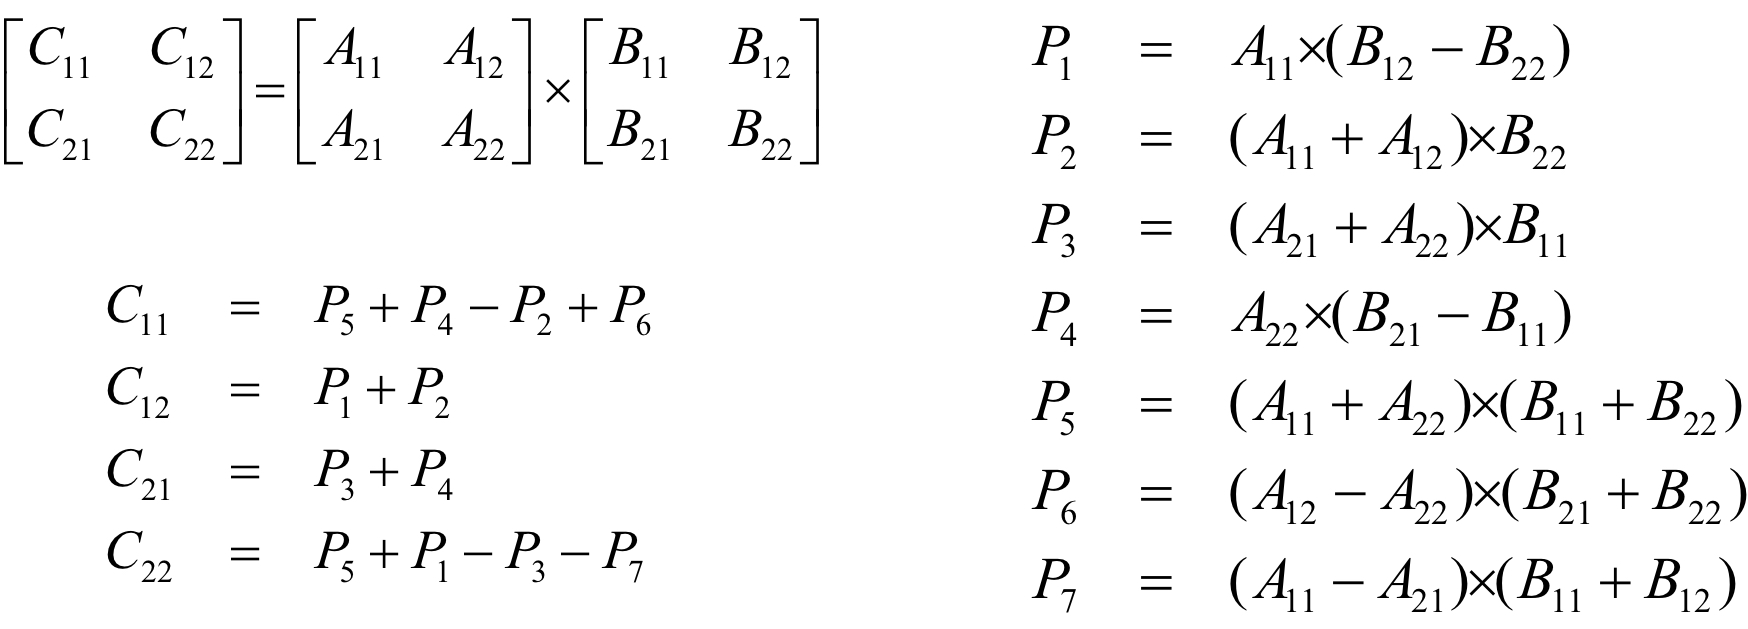
\includegraphics[scale=0.19]{images/02-matrix-mult.jpg}
    \end{center}
    
    And this reduce the running time down to 
    $O(n^{\log_2 7})\approx O(n^{2.807})$.

    Again, many people are trying to reduce the time complexity 
    and another competition arose. 
    We would not go into details here.


\end{spacing}



\part{Calculus}

\chapter{Chapter 12: Partial Differentiation}

\chapter{Chapter 13: Application of Partial Derivatives}


\begin{spacing}{1.3}

    \section{Extreme Values}
    {\blue Recall that in single variable calculus:

    $x_1$ is a {\it relative} maximum point, if $f'(x_1)=0$ and $f''(x_1)<0$,\\
    $x_2$ is a {\it relative} minimum point, if $f'(x_2)=0$ and $f''(x_2)>0$.
    }

    Similarly, in multi-variable calculus, the {\bf critical point} is where 
    \begin{center}
        \boxed{$$\disp \nabla f(\rr_0)=(f_{x_1}(\rr_0), f_{x_2}(\rr_0),\cdots,f_{x_n}(\rr_0))={\bf 0}$$}
    \end{center}
    

    And, if $h$ has a {\bf relative extremum} at a point $\rr_0$, then $\rr_0$ is a {\bf critical point},
    and $\nabla f(\rr_0)={\bf 0}$.
    However, if $\rr_0$ is a critical point, we {\it cannot infer} that $\rr_0$ is a relative extremum.
    The reason is similar in single variable calculus.

    \vspace{0.4in}
    Different from single variable, a critical point which {\it is not a relative extremum} is a {\bf saddle point}.
    
    \newpage
    \begin{center}
        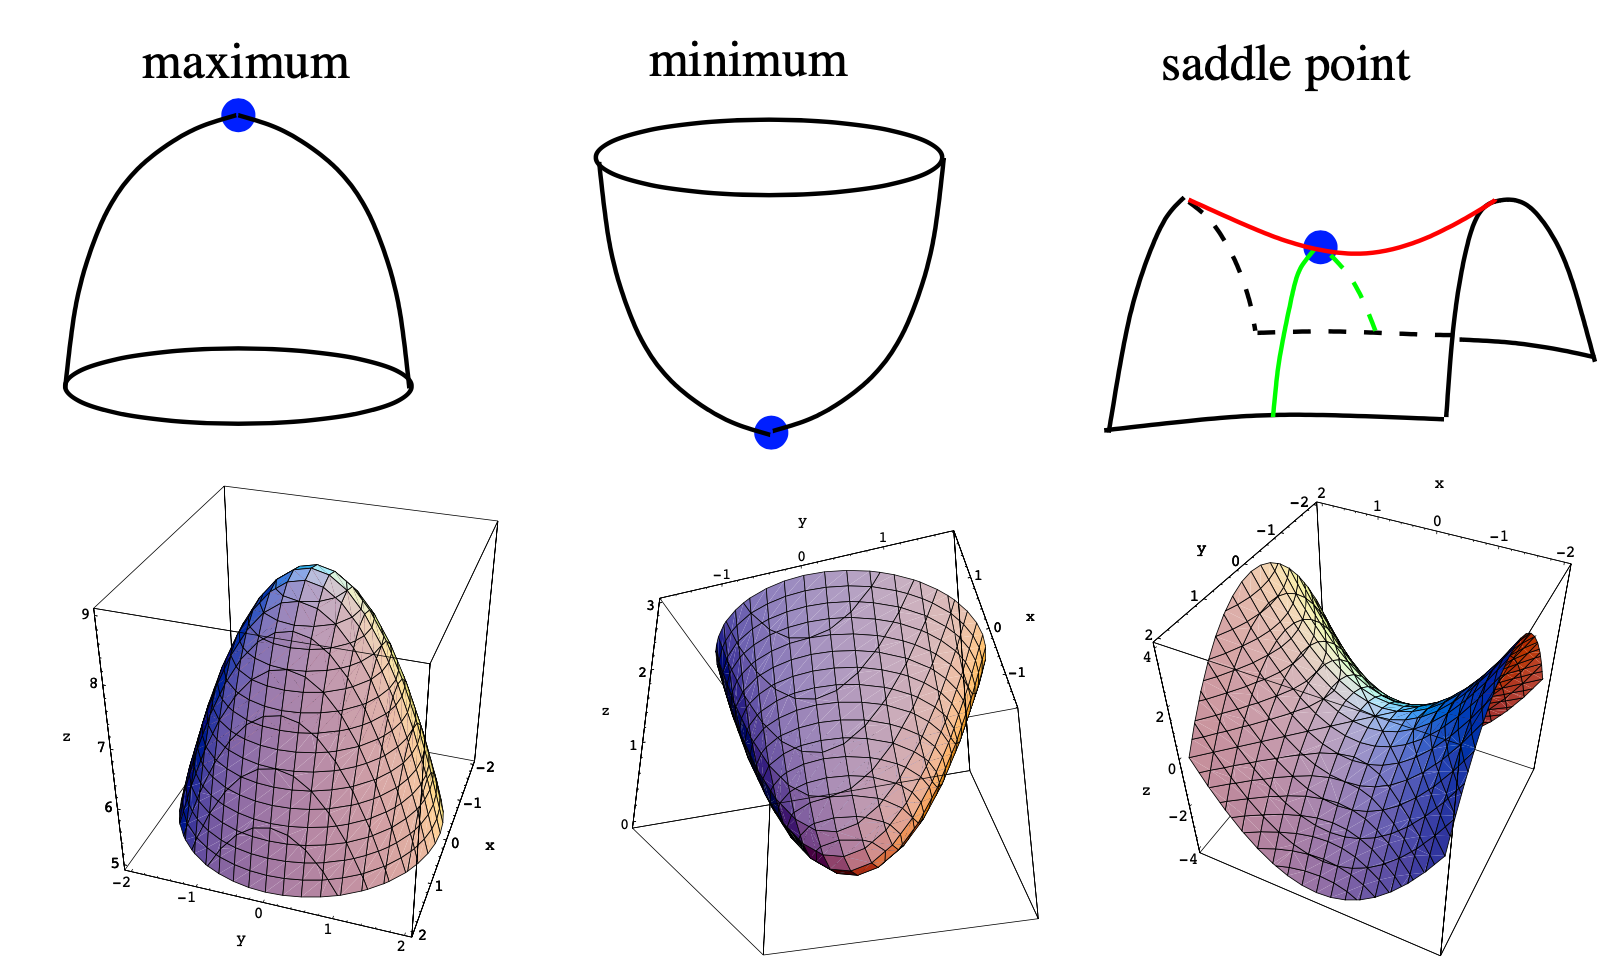
\includegraphics[scale=0.4]{images/Ch13-saddle.png}
    \end{center}

    However, to classify the critical points, we need the {\bf second derivative test}, or {\bf D-test}.

    \vspace{0.3in}
    {\bf Second Derivative Test}

    Suppose $f(x, y)$ has a critical point at $\mathbf{r}_{0}=\left(x_{0}, y_{0}\right)$ 
    (i.e. $\left.\nabla f\left(\mathbf{r}_{0}\right)=\mathbf{0}\right)$ and the second partial 
    derivative of $f(x, y)$ are continuous in a disk with center $\mathbf{r}_{0}=\left(x_{0}, y_{0}\right) .$ Let
    \begin{center}
        \boxed{$$\disp 
        D=\left|\begin{array}{ll}
        f_{x x}\left(\mathbf{r}_{0}\right) & f_{x y}\left(\mathbf{r}_{0}\right) \\
        f_{y x}\left(\mathbf{r}_{0}\right) & f_{y y}\left(\mathbf{r}_{0}\right)
        \end{array}\right|=f_{x x}\left(\mathbf{r}_{0}\right) f_{y y}\left(\mathbf{r}_{0}\right)-f_{x y}^{2}\left(\mathbf{r}_{0}\right)
        $$}
    \end{center}
    
    \begin{center}
        \begin{tabular}{c|c|c}
            \hline\hline 
            $D$ & $f_{x x}\left(\mathbf{r}_{0}\right)$ or $f_{y y}\left(\mathbf{r}_{0}\right)$ & nature of $\mathbf{r}_{0}$ \\\hline\hline
            $>0$ & $>0$ & relative minimum \\\hline
            $>0$ & $<0$ & relative maximum \\\hline
            $<0$ & & saddle point \\\hline
            $=0$ & & no conclusion can be drawn \\\hline
        \end{tabular}
    \end{center}
    
    \vspace{0.4in}
    {\it I'd like to omit the proof of D-Test here.}

    \newpage
    {\blue This example shows basic use of D-Test.}

    \eg Find the relative minima and maxima of $f(x, y)=x^{3}+y^{3}-3 x-12 y+20$.
    $$
    f_{x}=3 x^{2}-3 \quad \text { and } \quad f_{y}=3 y^{2}-12
    $$

    \sol 
    For critical points, $f_{x}=f_{y}=0 \quad \Rightarrow \quad x=\pm 1, y=\pm 2$.

    $\therefore (1,2),(-1,2),(1,-2),(-1,-2)$ are critical points.

    To apply D-Test, compute:
    $f_{xx}=6x, f_{yy}=6y, f_{xy}=0$, hence $D=f_{xx}\cdot f_{yy}-(f_{xy})^2= 36xy$

    \begin{center}
        \begin{tabular}{c|c|c|c|c|c}\hline\hline
            Point & $f_{xx}$ & $f_{yy}$ & $f_{xy}$ & $D$ & Type\\\hline\hline
            $(1,2)$ & 6 & 12 & 0 & 72 & min \\\hline
            $(-1,2)$ & $-6$ & 12 & 0 & $-72$ & saddle\\\hline
            $(1,-2)$ & 6 & $-12$ & 0 & $-72$ & saddle\\\hline
            $(-1,-2)$ & $-6$ & $-12$ & 0 & 72 & max\\\hline
        \end{tabular}
    \end{center}



    \newpage
    {\blue This example shows how to find extrema on a {\it closed} and {\it bounded} region.}

    \eg Find the absolute extrema of the function
    $$z=f(x, y)=x y-x-3 y$$
    on the {\it closed} and {\it bounded} set $R$, where $R$ is the triangular 
    region with vertices $(0,0),(0,4)$ and $(5,0)$.

    \sol $f_x=y-1, f_y=x-3, f_{xy}=f_{yx}=1, f_{xx}=f_{yy}=0, D=-1$

    For critical points, $\nabla f=(f_x, f_y)=(0,0) \Rightarrow x=3, y=1$.

    This point is inside the domain. But we still need to find possible 
    extreme points {\it on the boundary of domain}.

    {\bf (1)} Along $OA:$, $\rr_0=(0,0), \rr_1=(5,0)$, so the parametric representation 
    of line $OA$ is:
    $$\rr(t)=(1-t)\rr_0+t\rr_1,=(5t, 0),\ t\in [0,1]$$
    hence $z=f(\rr(t))=-5t,\ t\in [0,1]$

    So along $OA$, the possible extreme points are $(0,0)$ and $(5,0)$.

    {\bf (2)} Along $OB:$, similarly, $\rr(t)=(0, 4t),\ t\in [0,1]$, 
    $z=f(\rr)=-12t$,

    So along $OB$, the possible extreme points are $(0,0)$ and $(0,4)$.

    {\bf (3)} Along $AB:$ $\rr(t)=(5-5t, 4t),\ t\in [0,1]$,
    $z=-20t^2+13t-5,\ t\in [0,1]$

    There is one critical point on $AB$, when $dz/dx=0$, at $\left(\dfrac{27}{8}, \dfrac{13}{10}\right)$.

    Then we compute the value of all possible extremum points,
    \begin{center}
        \begin{tabular}{c|c}\hline\hline
            $(x,y)$ & $f(x,y)$ \\\hline\hline
            $(3,1)$ & $-3$\\\hline
            $\left(\dfrac{27}{8}, \dfrac{13}{10}\right)$ & $-\dfrac{231}{80}$\\\hline
            $(0,0)$ & 0 \\\hline
            $(5,0)$ & $-5$ \\\hline
            $(0,4)$ & $-12$ \\\hline
        \end{tabular}
    \end{center}

    Therefore, absolute maximum value is 0 which occurs at $(0,0)$,
    absolute minimum value is $-12$ which occurs at $(0,4)$. 


    \vspace{0.2in}
    {\blue This example converts the problem to max/min problem.}

    \eg Find the points on the surface $z^2=xy+1$ that are closest to the origin.

    \sol $d^2=(x-0)^2+(y-0)^2+(z-0)^2=x^2+y^2+xy+1=f(x,y)$, only need to minimize this function.


    \newpage
    {\blue This is a more comprehensive and tricker problem.}

    \eg Find absolute minimum and maximum value of $f(x,y)=2x^3+y^4$ on the set 
    $D=\{(x,y)|x^2+y^2\le 1\}$.

    \sol First, find the critical point of $f(x,y)$ on entire $xy$ plane.

    $f_x=6x^2, f_y=4y^3$, critical points: $f_x=f_y=0\Rightarrow x=y=0$, and $f(0,0)=0$.

    Then, on the circle $x^2+y^2=1$, eliminate $y$, we have:
    \begin{align*}
        g(x) &= f(x,y)=x^4+2x^3-2x^2+1,\ -1\le x\le 1\\
        g'(x) &= 4x^3+6x-4x=0
    \end{align*}
    the equation has solutions: $(x,y)=(0, \pm 1), \left(\frac{1}{2}, \frac{\sqrt{3}}{2}\right)$,
    to check each of them:
    $$f(0, \pm 1)=g(0)=1,\ f\left(\frac{1}{2}, \frac{\sqrt{3}}{2}\right)=g\left(\frac{1}{2}\right)=\frac{13}{16}$$
    Also, we need to check the {\it endpoints}, (since we are looking for min/max point of $g(x)$ on $x\in [-1,1]$)
    $$g(1)=2,\ g(-1)=-2$$
    Therefore, the absolute minimum is $g(-1)=f(-1,0)=-2$, the absolute maximum is $g(1)=f(1,0)=2$.

    \vspace{0.5in}
    Notice that, if you are interested in the nature of the critical point at $(0,0)$, you may try $D$-test:
    $$D=f_{xx}f_{yy}-f_{xy}^2=144xy^2=0\ \text{\ ,\ at (0,0)}$$
    so the $D$-test fails, we have to use other methods to determine it:

    In the plane $y=0$, $f(x,0)=2x^3$, and in the plane $x=0$, $f(0,y)=y^4$.
    \begin{center}
        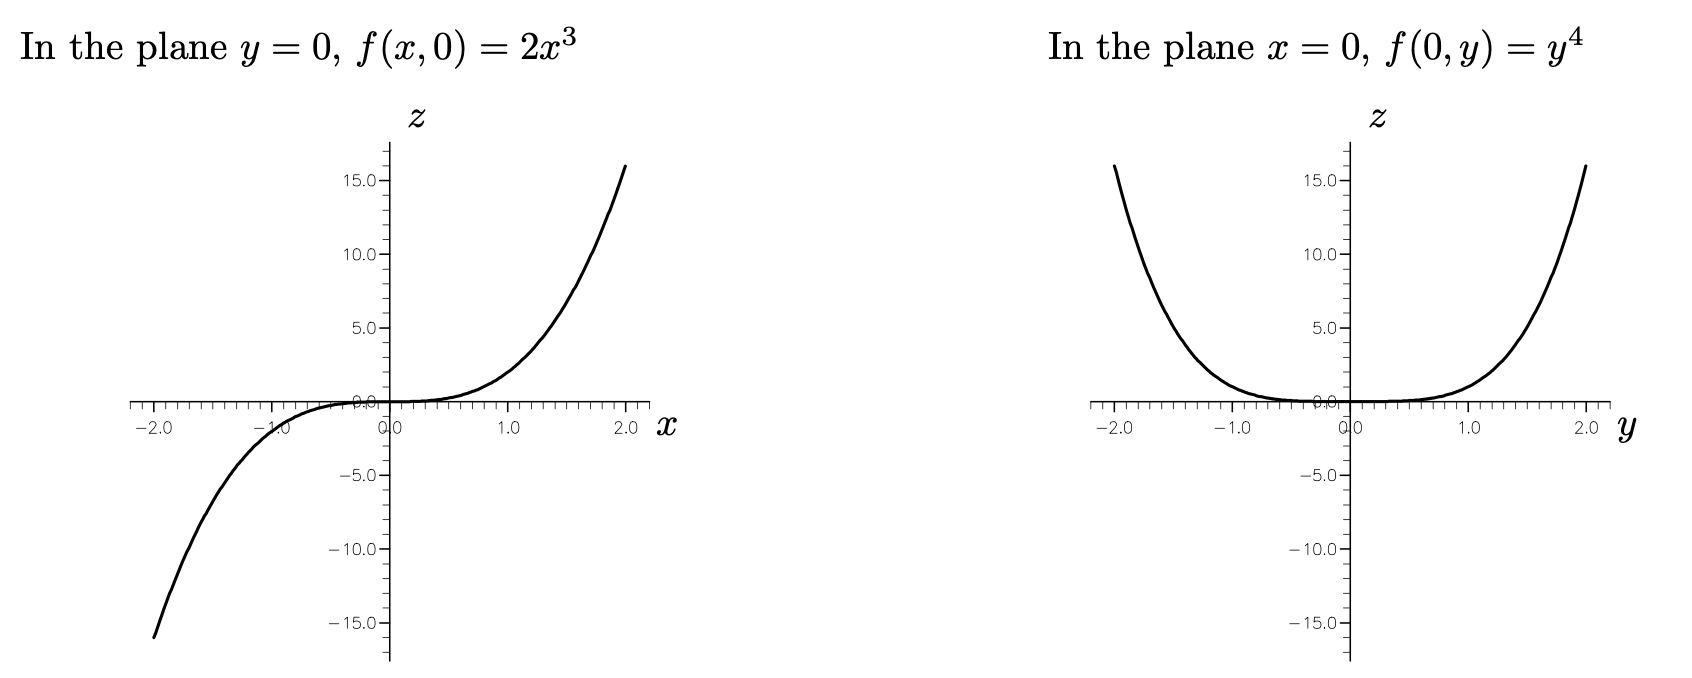
\includegraphics[scale=0.46]{images/Ch13-ex1.4.png}
    \end{center}
    Thus, the critical point is a {\it saddle point.}


    \newpage
    \section{Lagrange multipliers}

    {\blue Motivation: sometimes we want to maximize/minimize $f(x,y)$ subject to $g(x,y)=k$.}

    {\bf How to find the maximum or minimum value?}
    \begin{enumerate}
        \item Find all values of $\mathbf{r}$ and $\lambda$ such that
        $$\nabla f(\mathbf{r})=\lambda \nabla g(\mathbf{r})$$
        and $$g(\mathbf{r})=k$$
        \item Evaluate $f$ at all the points $\mathbf{r}$ that arise from step (1). 
        The largest (smallest) of these values is the maximum (min) value of $f$.
    \end{enumerate}

    {\it \textbf{Remark:}} Lagrange's method only finds critical points, 
    it {\it does not tell} whether the function is maximized or minimized.

    \vspace{0.5in}
    {\bf Proof of Lagrange's method:}

    Notice that, maximizing or minimizing a function $f(x_1,x_2,\cdots,x_n)$
    subject to a constraint of $g(x_1,x_2,\cdots,x_n)=k$ is to restrict 
    the point $(x_1,x_2,\cdots,x_n)$ to lie on the {\it level surface} $S$
    given by $g(x_1,x_2,\cdots,x_n)=k$. For example, if $n=2$, 
    maximize(or minimize) $z=f(x,y)$ subject to constraint curve $C:g(x,y)=k$
    (shown in {\green green}) is to restrict the point $(x,y)$ to lie on the {\red red} curve.
    \begin{center}
        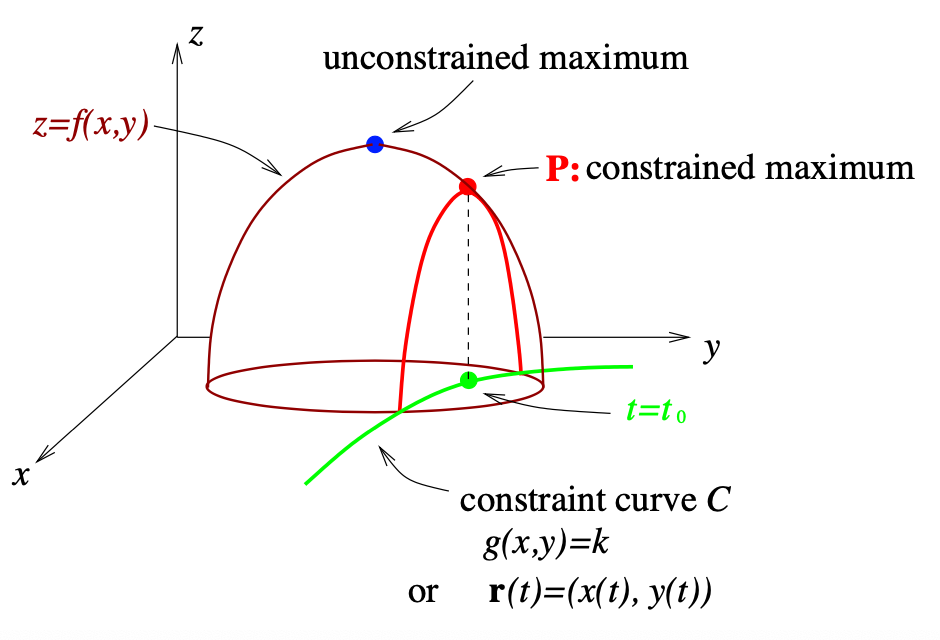
\includegraphics[scale=0.45]{images/Ch13-lag-proof.png}
    \end{center}
    Suppose $z$ has a maximum value at a point $\mathbf{P}$, and let $C$ be the {\it constraint curve} 
    with vector equation
    $$\mathbf{r}(t)=x(t) \mathbf{i}+y(t) \mathbf{j} \quad \text { be on } \quad g(x, y)=k \text {. }$$
    Assume also that at the point $\mathbf{P}, t=t_{0}$. 
    
    Since on the constraint curve $C: z(t)=f(x(t), y(t))$,

    and the point $\bf P$ should be a critical point. By using the chain rule,
    $$\begin{aligned}
    \frac{d z}{d t} &=\frac{\partial f}{\partial x} \frac{d x}{d t}+\frac{\partial f}{\partial y} \frac{d y}{d t} \\
    &=\left(\frac{\partial f}{\partial x}, \frac{\partial f}{\partial y}\right) \cdot\left(\frac{d x}{d t}, \frac{d y}{d t}\right) \\
    &=\nabla f \cdot \mathbf{r}^{\prime}(t)
    \end{aligned}$$
    Then at the point $\mathbf{P}$,
    $$\left.\frac{d z}{d t}\right|_{t=t_{0}}=\nabla f\left(x\left(t_{0}\right), y\left(t_{0}\right)\right) 
    \cdot \mathbf{r}^{\prime}\left(t_{0}\right)=0 \quad \text { (since {\bf P} is critical point) }$$

    Therefore, 
    $$\nabla f\left(x\left(t_{0}\right), y\left(t_{0}\right)\right)  \perp \mathbf{r}^{\prime}\left(t_{0}\right)$$
    
    Moreover, since $\nabla g$ is normal vector to the level set,
    $$\nabla g\left(x\left(t_{0}\right), y\left(t_{0}\right)\right)  \perp \mathbf{r}^{\prime}\left(t_{0}\right) $$
    Therefore, $\nabla f \parallel \nabla g$, $\nabla f=\lambda \nabla g$.
    
    The number $\lambda$ is called a Lagrange multiplier.

    \newpage
    {\blue This example shows how to use Lagrange's Method.}

    \eg Find the extreme values of $f(x, y)=x^{2}-y^{2}$ subject to $x^{2}+y^{2}=1$.
    
    \sol Find $x, y$ and $\lambda$ such that
    $\nabla f=\lambda \nabla g$, where $g=x^{2}+y^{2}=1$(constant) 
    $$2 x \mathbf{i}-2 y \mathbf{j}=\lambda(2 x \mathbf{i}+2 y \mathbf{j})$$
    , which gives
    $$
    \left\{\begin{array}{rl}
        2x= & \lambda \cdot 2x\\
        -2y= & \lambda \cdot 2y
    \end{array} \right.  \qquad \Rightarrow \qquad 
    \left\{\begin{array}{lcl}
        \lambda = 1 & {\rm or} & x=0\\
        \lambda = -1 & {\rm or} & y=0\\
    \end{array} \right.
    $$
    From $x^2+y^2=1$, we have:
    \begin{align*}
        &x=0,\ y=\pm 1,\ \lambda = -1\\
        &y=0,\ x=\pm 1,\ \lambda = 1
    \end{align*}
    Therefore, $f$ has possible extreme values at point $(0,1),(0,-1),(-1,0)$ and $(1,0)$. Evaluating $f$ at these four points, we find that
    $$\begin{aligned}
        &f(0,1)=f(0,-1)=-1 \quad(\min ) \\
        &f(1,0)=f(-1,0)=1 \quad(\max )
    \end{aligned}$$



    \newpage
    {\bf Interpretation of $\lambda$}

    {\blue {\it This will not be tested in exam.}}

    Actually, $\lambda$ has an interpretation which can be very useful.

    Suppose $M$ is the optimal value of $f(x, y)$ subject to the constraint $g(x, y)=c.$

    Then $f(x, y)=M$ for some ordered pair $(x, y)$ that satisfies the three Lagrangian equations
    $$\begin{array}{r}
        f_{x}-\lambda g_{x}=0 \\
        f_{y}-\lambda g_{y}=0 \\
        g=c
    \end{array}$$
    Since $M=f(x, y)$
    $$\begin{aligned}
    \frac{d M}{d c} &=\frac{\partial f}{\partial x} \frac{d x}{d c}+\frac{\partial f}{\partial y} \cdot \frac{d y}{d c} \\
    &=f_{x} \frac{d x}{d c}+f_{y} \frac{d y}{d c} \\
    &=\lambda g_{x} \frac{d x}{d c}+\lambda g_{y} \frac{d y}{d c} \\
    &=\lambda\left(g_{x} \frac{d x}{d c}+g_{y} \frac{d y}{d c}\right) \\
    &=\lambda \frac{d g}{d c}=\lambda
    \end{aligned}$$
    where $d M / d c$ is evaluated at the optimal solution values. In other words, $\lambda$ measures 
    the {\it sensitivity} of the optimal value of $f$ to change in $c$.
    \begin{center}
        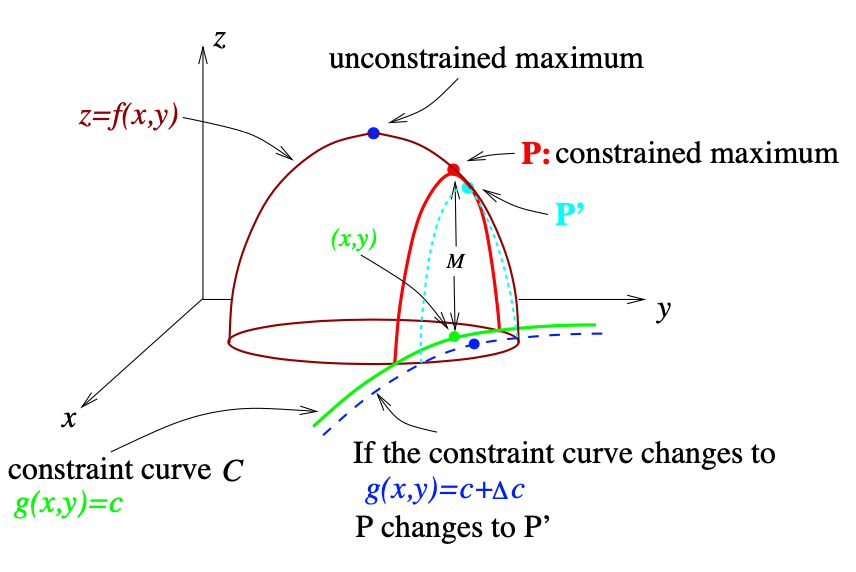
\includegraphics[scale=0.53]{images/Ch13-intepret-lambda.png}
    \end{center}

    \newpage
    {\blue The example below shows the application of $\lambda$.}
    
    \eg Use Lagrangian multiplier to find the maximum and minimum values of the function
    $f(x, y)=4 x^{3}+y^{2}$
    subject to the constraint $2x^{2}+y^{2}=1$.

    If the constraint equation changes to $2 x^{2}+y^{2}=0.9$, 
    estimate how this changes will affect the maximum and minimum values of $f$.

    \sol Let $g(x,y)=2x^2+y^2=1=c$, then for $\nabla f = \lambda \nabla g$, we have
    $(12x^2, 2y)=\lambda (4x, 2y)$, i.e., 
    \begin{align*}
        12x^2 &= \lambda 4x\\
        2y &= \lambda 2y\\
        2x^2+y^2&=1
    \end{align*}
    From the second equation, if $y\ne 0$, then $\lambda = 1$, substitute into the other two equations, 
    we get $\disp (x,y)=(0, \pm 1){\rm \ or\ } \left(\frac{1}{3},\pm \frac{\sqrt{7}}{3}\right)$

    However, if $y=0$, then from third equation, $\disp x=\pm \frac{\sqrt{2}}{2}$, substitute to first eq, 
    we get:
    $$\begin{array}{lll}
        \lambda = \dfrac{3\sqrt{2}}{2} & {\rm when} & x=\dfrac{\sqrt{2}}{2}\\
        \lambda = -\dfrac{3\sqrt{2}}{2} & {\rm when} & x=-\dfrac{\sqrt{2}}{2}
    \end{array}$$

    \begin{center}
        \begin{tabular}{|c|c|c|c|}\hline
            $\lambda$ & $(x,y)$ & $f(x,y)$ & nature \\\hline
            1 & $(0, \pm 1)$ & 1 &  \\\hline
            1 & $\disp \left(\frac{1}{3},\pm \frac{\sqrt{7}}{3}\right)$ & $\disp \frac{25}{27}$ &  \\\hline
            $\disp \frac{3\sqrt{2}}{2}$ & $\disp \left(\frac{\sqrt{2}}{2}, 0\right)$ & $\sqrt{2}$ & max \\\hline
            $\disp -\frac{3\sqrt{2}}{2}$ & $\disp \left(-\frac{\sqrt{2}}{2}, 0\right)$ & $-\sqrt{2}$ & min \\\hline        
        \end{tabular}
    \end{center}
    Since $\disp \frac{dM}{dc}=\lambda$, so $\Delta M\approx \lambda \Delta c$, in this case, $\Delta c=-0.1$, so 
    at min point, 
    $$\Delta M=-\frac{3\sqrt{2}}{2}\cdot (-0.1)=\frac{3\sqrt{2}}{20}\quad {\rm (increase)}$$
    at max point,
    $$\Delta M=\frac{3\sqrt{2}}{2}\cdot (-0.1)=-\frac{3\sqrt{2}}{20}\quad {\rm (decrease)}$$


\end{spacing}


\chapter{Chapter 14: Multiple Integrations}


\begin{spacing}{1.3}

    \section{Double Integrals Over Rectangles}

    Recall that in single variable calculus, we divided a region into 
    thin rectangles and use the {\bf Riemann Sum} as integral.
    \begin{center}
        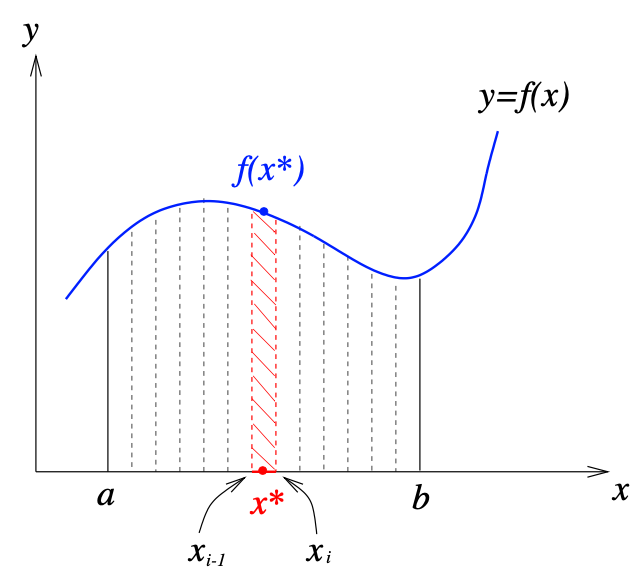
\includegraphics[scale=0.45]{images/Ch14-intro.png}
    \end{center}
    $$\int_a^b f(x)dx=\lim_{n\rightarrow \infty}\sum_{i=1}^n f(x_i^\star)\delta x_i$$
    
    Actually, instead of thin rectangles, we can use {\it small rectangles} to cover the area.

    \eg Find the area bounded by $y=x$, $x=1$ and $y=0$.

    \sol (1) View the area as bounded by {\it upper curve} and {\it lower curve}.
    

    \tikzset{every picture/.style={line width=0.75pt}} %set default line width to 0.75pt        
    \begin{center}
        \begin{tikzpicture}[x=0.75pt,y=0.75pt,yscale=-1,xscale=1]
            %uncomment if require: \path (0,300); %set diagram left start at 0, and has height of 300
        
            %Shape: Axis 2D [id:dp3896868200656678] 
            \draw  (68,207) -- (243,207)(85.5,66) -- (85.5,222.67) (236,202) -- (243,207) -- (236,212) (80.5,73) -- (85.5,66) -- (90.5,73)  ;
            %Straight Lines [id:da8649162174794645] 
            \draw [color={rgb, 255:red, 255; green, 0; blue, 0 }  ,draw opacity=1 ]   (85.5,207) -- (175,117.5) ;
            %Straight Lines [id:da8918167425471388] 
            \draw    (175,117.5) -- (175,206.67) ;
            %Straight Lines [id:da20672609799626906] 
            \draw [color={rgb, 255:red, 0; green, 255; blue, 0 }  ,draw opacity=1 ]   (85.5,207) -- (175,206.67) ;
            %Curve Lines [id:da7341114132390345] 
            \draw    (110.33,144) .. controls (105.74,149.25) and (78.5,160.33) .. (114.64,172.76) ;
            \draw [shift={(116.33,173.33)}, rotate = 198.14] [color={rgb, 255:red, 0; green, 0; blue, 0 }  ][line width=0.75]    (10.93,-3.29) .. controls (6.95,-1.4) and (3.31,-0.3) .. (0,0) .. controls (3.31,0.3) and (6.95,1.4) .. (10.93,3.29)   ;
            %Curve Lines [id:da6058369715667598] 
            \draw    (123,231.33) .. controls (118.4,236.59) and (91.81,226.96) .. (120.96,211.38) ;
            \draw [shift={(122.33,210.67)}, rotate = 512.95] [color={rgb, 255:red, 0; green, 0; blue, 0 }  ][line width=0.75]    (10.93,-3.29) .. controls (6.95,-1.4) and (3.31,-0.3) .. (0,0) .. controls (3.31,0.3) and (6.95,1.4) .. (10.93,3.29)   ;
            %Shape: Rectangle [id:dp5051745743053773] 
            \draw  [color={rgb, 255:red, 0; green, 0; blue, 0 }  ,draw opacity=1 ][fill={rgb, 255:red, 74; green, 144; blue, 226 }  ,fill opacity=0.51 ][dash pattern={on 0.84pt off 2.51pt}][line width=0.75]  (134,168.67) -- (149,168.67) -- (149,180) -- (134,180) -- cycle ;
            %Shape: Axis 2D [id:dp8934264331658603] 
            \draw  (296,207) -- (471,207)(313.5,66) -- (313.5,222.67) (464,202) -- (471,207) -- (464,212) (308.5,73) -- (313.5,66) -- (318.5,73)  ;
            %Straight Lines [id:da7529215091369386] 
            \draw [color={rgb, 255:red, 255; green, 0; blue, 0 }  ,draw opacity=1 ]   (313.5,207) -- (403,117.5) ;
            %Straight Lines [id:da6761798304849251] 
            \draw    (403,117.5) -- (403,206.67) ;
            %Straight Lines [id:da16391256653051056] 
            \draw [color={rgb, 255:red, 0; green, 255; blue, 0 }  ,draw opacity=1 ]   (313.5,207) -- (403,206.67) ;
            %Curve Lines [id:da35417352536646507] 
            \draw    (338.33,144) .. controls (333.74,149.25) and (306.5,160.33) .. (342.64,172.76) ;
            \draw [shift={(344.33,173.33)}, rotate = 198.14] [color={rgb, 255:red, 0; green, 0; blue, 0 }  ][line width=0.75]    (10.93,-3.29) .. controls (6.95,-1.4) and (3.31,-0.3) .. (0,0) .. controls (3.31,0.3) and (6.95,1.4) .. (10.93,3.29)   ;
            %Curve Lines [id:da5929159990416739] 
            \draw    (351,231.33) .. controls (346.4,236.59) and (319.81,226.96) .. (348.96,211.38) ;
            \draw [shift={(350.33,210.67)}, rotate = 512.95] [color={rgb, 255:red, 0; green, 0; blue, 0 }  ][line width=0.75]    (10.93,-3.29) .. controls (6.95,-1.4) and (3.31,-0.3) .. (0,0) .. controls (3.31,0.3) and (6.95,1.4) .. (10.93,3.29)   ;
            %Shape: Trapezoid [id:dp507673701497652] 
            \draw  [fill={rgb, 255:red, 74; green, 144; blue, 226 }  ,fill opacity=0.49 ][dash pattern={on 0.84pt off 2.51pt}] (381,206.11) -- (366.25,206.11) -- (366.25,155.72) -- (381,140.15) -- cycle ;
        
            % Text Node
            \draw (70,59.07) node [anchor=north west][inner sep=0.75pt]    {$y$};
            % Text Node
            \draw (246.67,199.07) node [anchor=north west][inner sep=0.75pt]    {$x$};
            % Text Node
            \draw (135.33,105.73) node [anchor=north west][inner sep=0.75pt]  [font=\small]  {$y=x$};
            % Text Node
            \draw (178.67,157.4) node [anchor=north west][inner sep=0.75pt]  [font=\small]  {$x=1$};
            % Text Node
            \draw (88.67,125.33) node [anchor=north west][inner sep=0.75pt]  [color={rgb, 255:red, 255; green, 0; blue, 0 }  ,opacity=1 ] [align=left] {{\footnotesize upper curve}};
            % Text Node
            \draw (126.67,220.67) node [anchor=north west][inner sep=0.75pt]  [color={rgb, 255:red, 0; green, 255; blue, 0 }  ,opacity=1 ] [align=left] {{\footnotesize lower curve}};
            % Text Node
            \draw (134,178.73) node [anchor=north west][inner sep=0.75pt]  [font=\footnotesize]  {$dx$};
            % Text Node
            \draw (150,168.07) node [anchor=north west][inner sep=0.75pt]  [font=\footnotesize]  {$dy$};
            % Text Node
            \draw (298,59.07) node [anchor=north west][inner sep=0.75pt]    {$y$};
            % Text Node
            \draw (474.67,199.07) node [anchor=north west][inner sep=0.75pt]    {$x$};
            % Text Node
            \draw (363.33,105.73) node [anchor=north west][inner sep=0.75pt]  [font=\small]  {$y=x$};
            % Text Node
            \draw (406.67,157.4) node [anchor=north west][inner sep=0.75pt]  [font=\small]  {$x=1$};
            % Text Node
            \draw (316.67,125.33) node [anchor=north west][inner sep=0.75pt]  [color={rgb, 255:red, 255; green, 0; blue, 0 }  ,opacity=1 ] [align=left] {{\footnotesize upper curve}};
            % Text Node
            \draw (354.67,220.67) node [anchor=north west][inner sep=0.75pt]  [color={rgb, 255:red, 0; green, 255; blue, 0 }  ,opacity=1 ] [align=left] {{\footnotesize lower curve}};
            % Text Node
            \draw (367.33,206.73) node [anchor=north west][inner sep=0.75pt]  [font=\footnotesize]  {$dx$};
        \end{tikzpicture}
    \end{center}
    

    For the {\it small rectangles} with $dA=dxdy=dydx$, we first move it vertically,
    the lower bound is $y=0$, and the upper bound is $y=x$, hence $\disp \int_0^x dy$
    is the shaded area in right image above.

    Then we move the shaded area horizontally, the left bound is point $x=0$, while 
    the right bound is point $x=1$, thus the total area is: 
    $$A=\int_0^1 \int_0^x dydx=\left. \int_0^1 y \right\vert_0^x dx=\int_0^1 xdx=\frac{1}{2}$$

    (2) Alternatively, we can first move the rectangle horizontally, hitting 
    {\it left curve} $x=y$ and {\it right curve} $x=1$, hence the shaded area is 
    $\disp \int_y^1 dx$. {\red note here we integral $dx$ first, so when hitting 
    the boundaries, we need to check $x$ equals to what, i.e. $x=f(y)$.}
    For example, here the two bounds are $x=y$ and $x=1$.
    \begin{center}
        \begin{tikzpicture}[x=0.75pt,y=0.75pt,yscale=-1,xscale=1]
        %uncomment if require: \path (0,300); %set diagram left start at 0, and has height of 300

        %Shape: Axis 2D [id:dp7553906893045521] 
        \draw  (88,227) -- (263,227)(105.5,86) -- (105.5,242.67) (256,222) -- (263,227) -- (256,232) (100.5,93) -- (105.5,86) -- (110.5,93)  ;
        %Straight Lines [id:da35403404535445815] 
        \draw [color={rgb, 255:red, 255; green, 0; blue, 0 }  ,draw opacity=1 ]   (105.5,227) -- (195,137.5) ;
        %Straight Lines [id:da01645345984200941] 
        \draw [color={rgb, 255:red, 0; green, 255; blue, 0 }  ,draw opacity=1 ][fill={rgb, 255:red, 0; green, 255; blue, 0 }  ,fill opacity=1 ]   (195,137.5) -- (195,226.67) ;
        %Curve Lines [id:da1854977378917313] 
        \draw    (130.33,164) .. controls (125.74,169.25) and (98.5,180.33) .. (134.64,192.76) ;
        \draw [shift={(136.33,193.33)}, rotate = 198.14] [color={rgb, 255:red, 0; green, 0; blue, 0 }  ][line width=0.75]    (10.93,-3.29) .. controls (6.95,-1.4) and (3.31,-0.3) .. (0,0) .. controls (3.31,0.3) and (6.95,1.4) .. (10.93,3.29)   ;
        %Curve Lines [id:da04722306457844705] 
        \draw    (220.33,163.67) .. controls (220.98,157.82) and (222.9,149.43) .. (198.9,157.05) ;
        \draw [shift={(197,157.67)}, rotate = 341.57] [color={rgb, 255:red, 0; green, 0; blue, 0 }  ][line width=0.75]    (10.93,-3.29) .. controls (6.95,-1.4) and (3.31,-0.3) .. (0,0) .. controls (3.31,0.3) and (6.95,1.4) .. (10.93,3.29)   ;
        %Shape: Rectangle [id:dp32583575696458844] 
        \draw  [color={rgb, 255:red, 0; green, 0; blue, 0 }  ,draw opacity=1 ][fill={rgb, 255:red, 74; green, 144; blue, 226 }  ,fill opacity=0.51 ][dash pattern={on 0.84pt off 2.51pt}][line width=0.75]  (154,188.67) -- (169,188.67) -- (169,200) -- (154,200) -- cycle ;
        %Shape: Trapezoid [id:dp3210513944610718] 
        \draw  [fill={rgb, 255:red, 74; green, 144; blue, 226 }  ,fill opacity=0.49 ][dash pattern={on 0.84pt off 2.51pt}] (345.54,205.61) -- (360.82,190.64) -- (413.98,189.86) -- (411.49,204.65) -- cycle ;
        %Shape: Axis 2D [id:dp46120188682750873] 
        \draw  (306,227.67) -- (481,227.67)(323.5,86.67) -- (323.5,243.33) (474,222.67) -- (481,227.67) -- (474,232.67) (318.5,93.67) -- (323.5,86.67) -- (328.5,93.67)  ;
        %Straight Lines [id:da22273680492149706] 
        \draw [color={rgb, 255:red, 255; green, 0; blue, 0 }  ,draw opacity=1 ]   (323.5,227.67) -- (413,138.17) ;
        %Straight Lines [id:da8910127482619856] 
        \draw [color={rgb, 255:red, 0; green, 255; blue, 0 }  ,draw opacity=1 ][fill={rgb, 255:red, 0; green, 255; blue, 0 }  ,fill opacity=1 ]   (413,138.17) -- (413,227.33) ;
        %Curve Lines [id:da6790580082651905] 
        \draw    (348.33,164.67) .. controls (343.74,169.92) and (316.5,180.99) .. (352.64,193.43) ;
        \draw [shift={(354.33,194)}, rotate = 198.14] [color={rgb, 255:red, 0; green, 0; blue, 0 }  ][line width=0.75]    (10.93,-3.29) .. controls (6.95,-1.4) and (3.31,-0.3) .. (0,0) .. controls (3.31,0.3) and (6.95,1.4) .. (10.93,3.29)   ;
        %Curve Lines [id:da2701777279829498] 
        \draw    (438.33,164.33) .. controls (438.98,158.48) and (440.9,150.1) .. (416.9,157.72) ;
        \draw [shift={(415,158.33)}, rotate = 341.57] [color={rgb, 255:red, 0; green, 0; blue, 0 }  ][line width=0.75]    (10.93,-3.29) .. controls (6.95,-1.4) and (3.31,-0.3) .. (0,0) .. controls (3.31,0.3) and (6.95,1.4) .. (10.93,3.29)   ;

        % Text Node
        \draw (90,79.07) node [anchor=north west][inner sep=0.75pt]    {$y$};
        % Text Node
        \draw (266.67,219.07) node [anchor=north west][inner sep=0.75pt]    {$x$};
        % Text Node
        \draw (155.33,125.73) node [anchor=north west][inner sep=0.75pt]  [font=\small]  {$y=x$};
        % Text Node
        \draw (199.33,188.07) node [anchor=north west][inner sep=0.75pt]  [font=\small]  {$x=1$};
        % Text Node
        \draw (113.33,146.67) node [anchor=north west][inner sep=0.75pt]  [color={rgb, 255:red, 255; green, 0; blue, 0 }  ,opacity=1 ] [align=left] {{\footnotesize left curve}};
        % Text Node
        \draw (204,159.33) node [anchor=north west][inner sep=0.75pt]  [color={rgb, 255:red, 0; green, 255; blue, 0 }  ,opacity=1 ] [align=left] {{\footnotesize right curve}};
        % Text Node
        \draw (154,198.73) node [anchor=north west][inner sep=0.75pt]  [font=\footnotesize]  {$dx$};
        % Text Node
        \draw (170,188.07) node [anchor=north west][inner sep=0.75pt]  [font=\footnotesize]  {$dy$};
        % Text Node
        \draw (414.65,189.92) node [anchor=north west][inner sep=0.75pt]  [font=\footnotesize]  {$dy$};
        % Text Node
        \draw (308,79.73) node [anchor=north west][inner sep=0.75pt]    {$y$};
        % Text Node
        \draw (484.67,219.73) node [anchor=north west][inner sep=0.75pt]    {$x$};
        % Text Node
        \draw (373.33,126.4) node [anchor=north west][inner sep=0.75pt]  [font=\small]  {$y=x$};
        % Text Node
        \draw (413.49,208.05) node [anchor=north west][inner sep=0.75pt]  [font=\small]  {$x=1$};
        % Text Node
        \draw (331.33,147.33) node [anchor=north west][inner sep=0.75pt]  [color={rgb, 255:red, 255; green, 0; blue, 0 }  ,opacity=1 ] [align=left] {{\footnotesize left curve}};
        % Text Node
        \draw (422,160) node [anchor=north west][inner sep=0.75pt]  [color={rgb, 255:red, 0; green, 255; blue, 0 }  ,opacity=1 ] [align=left] {{\footnotesize right curve}};
        \end{tikzpicture}
    \end{center}

    Then we move the shaded area vertically, hitting lower bound $y=0$(a point) and upper bound $y=1$(a point),
    hence the total area is: 
    $$A=\int_0^1 \int_y^1 dxdy=\left.\int_0^1  x \right\vert_y^1 dy=\int_0^1(1-y)dy=\frac{1}{2}$$

    \section{Double Integrals Over General Regions}

    \section{Double Integrals in Polar Coordinates}


    \newpage
    \section{Change of Variables in Integrals}

    Recall that in single variable calculus, we often use a {\it substitution} to simplify an integral.
    $$\int_a^b f(x)dx=\int_c^df(g(u))\cdot g'(u)\ du$$
    where $a=g(c)$ and $b=g(d)$. Notice that we can {\it view substitution as a kind of mapping}, and 
    the change-of-variable process introduces {\it an additional factor} $g'(u)$ into the integrand.

    This method can also be useful in multiple integrals. We have already seen one example: integration 
    in {\it polar coordinate}.
    $$\iint_{R} f(x, y) d A_{x y}=\iint_{S} f(r \cos \theta, r \sin \theta) r d r d \theta=\iint_{S} f(r \cos \theta, r \sin \theta) r d A_{r \theta}$$
    In this example, {\it the additional factor} is $r$.

    The {\it mapping} $T$ is shown as below: we transform the region $R$ into $S$, where $S$ is an rectangle in 
    $\theta r$-plane, which is easy to integrate.
    \begin{center}
        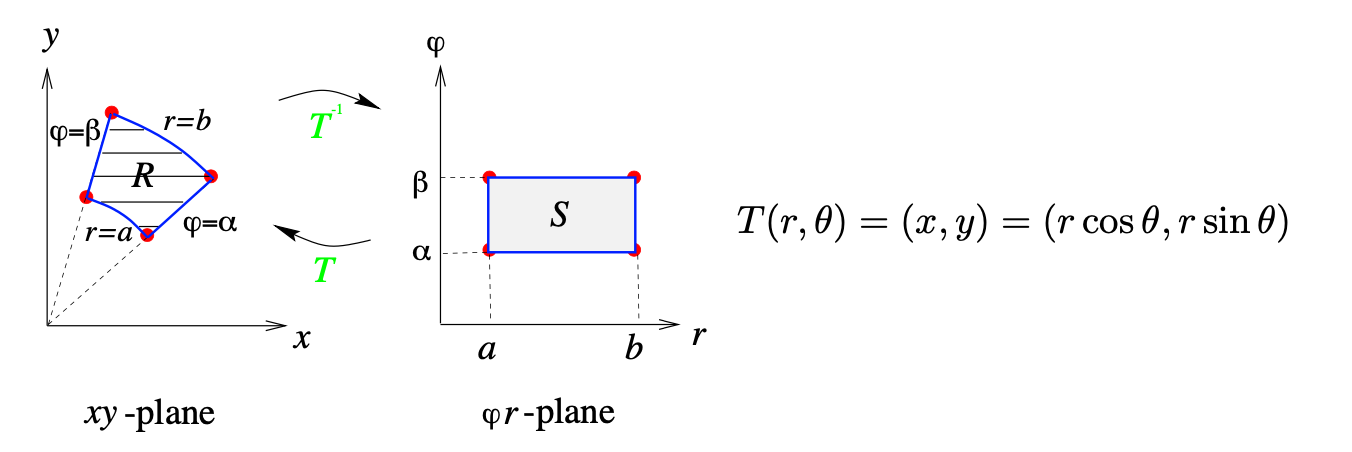
\includegraphics[scale=0.55]{images/Ch14-jacobians-polar-mapping.png}
    \end{center}

    \newpage
    \eg Find a change of variable.

    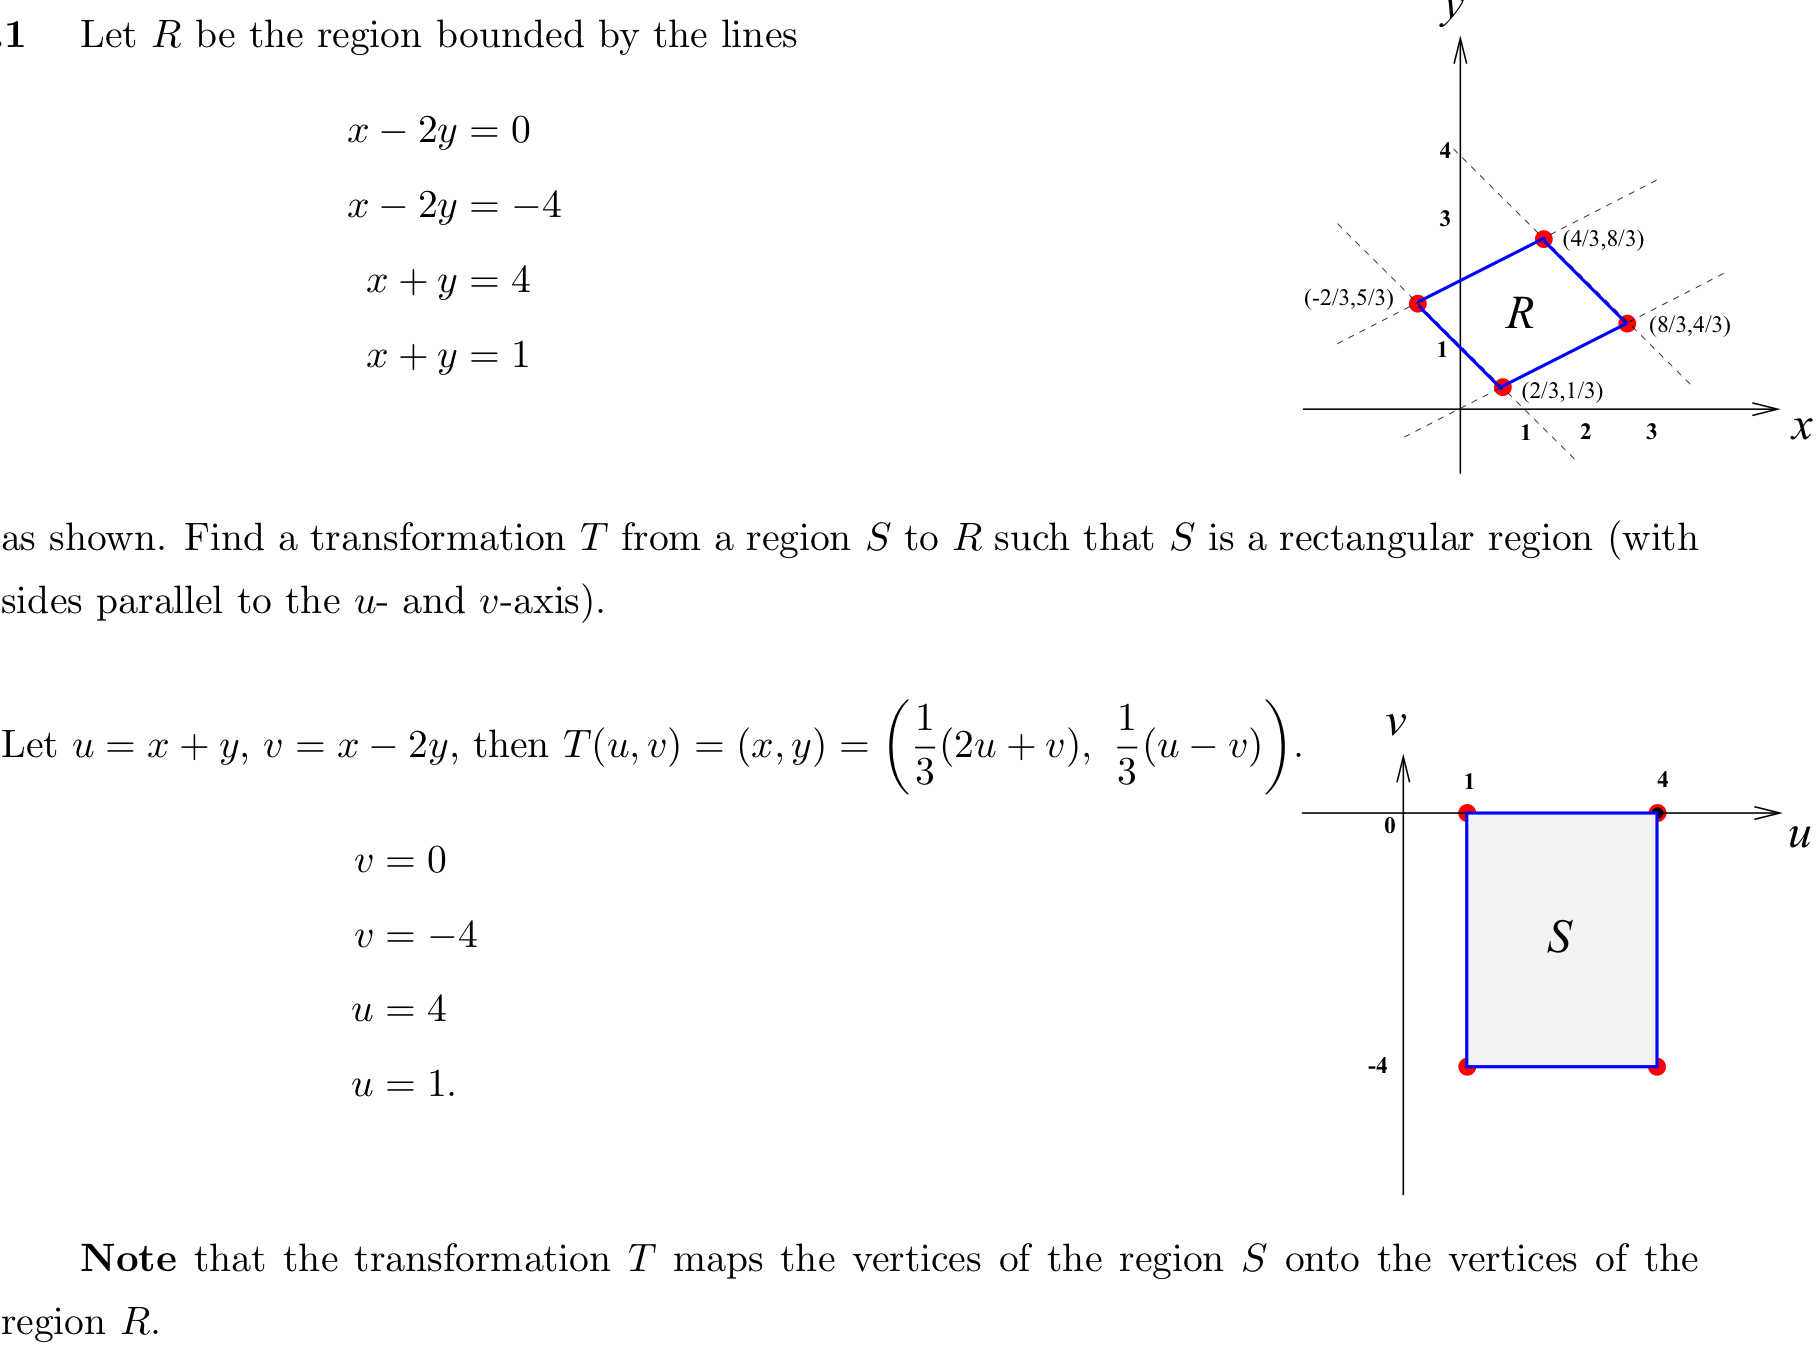
\includegraphics[scale=0.25]{images/Ch14-change-var-eg.jpeg}

    \newpage
    Now, to find $\disp \iint_R f(x,y) dxdy$, if we make the change of variables $x=g(u,v), y=h(u,v)$,
    then {\it we are mapping things in uv-plane onto things in xy-plane}. For mapping function 
    $T(u,v)=(g(u,v), h(u,v))=(x,y)$, and assume the area $S$ in $uv$-plane corresponds 
    to region $R$ in $xy$-plane, as shown below.

    \begin{center}
        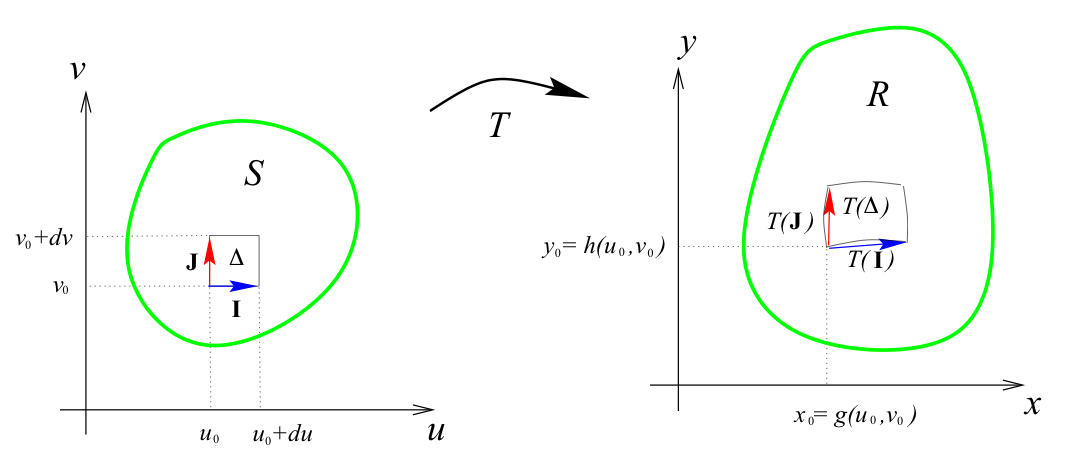
\includegraphics[scale=0.33]{images/Ch14-jacobian-mapping.jpeg}
    \end{center}

    We still use the method that integrate all ``small rectangles'', $\Delta$, as shown in $uv$-plane.
    Assume $\Delta$ locates at $(u_0,v_0)$ and has area $dA=dudv$. Let

    $\bf I$ be the vector from $\left(u_{0}, v_{0}\right)$ to $\left(u_{0}+d u, v_{0}\right)$ and\\
    $\mathbf{J}$ be the vector from $\left(u_{0}, v_{0}\right)$ to $\left(u_{0}, v_{0}+d v\right)$. 
    
    Then mapping $T$ ``takes'' $\bf I$ to the vector $T(\mathbf{I})$ from 
    $\left(g\left(u_{0}, v_{0}\right), h\left(u_{0}, v_{0}\right)\right)$ to 
    $\left(g\left(u_{0}+d u, v_{0}\right), h\left(u_{0}+d u, v_{0}\right)\right)$. 
    Notice the vector $T({\bf I})$ is {\it not necessary a straight vector}. Now
    $$
    \begin{aligned}
    T(\mathbf{I}) &=\left(g\left(u_{0}+d u, v_{0}\right)-g\left(u_{0}, v_{0}\right), h\left(u_{0}+d u, v_{0}\right)-h\left(u_{0}, v_{0}\right)\right) \\
    &=\left(\frac{g\left(u_{0}+d u, v_{0}\right)-g\left(u_{0}, v_{0}\right)}{d u}, \frac{h\left(u_{0}+d u, v_{0}\right)-h\left(u_{0}, v_{0}\right)}{d u}\right) d u \\
    &=\left(\frac{\partial g}{\partial u}, \frac{\partial h}{\partial u}\right) d u 
    \ \ {\rm \blue (for\ } {\blue  du\rightarrow 0)}
    \end{aligned}
    $$
    Similarly, $\disp T(\mathbf{J})=\left(\frac{\partial g}{\partial v}, \frac{\partial h}{\partial v}\right) dv$. 
    
    Then the area of $T(\Delta)$ is
    $$
    d x d y =\left\| T({\rm I})\cdot T({\rm J}) \right\|=\left| \left|\begin{array}{ll}
    \frac{\partial x}{\partial u} & \frac{\partial y}{\partial u} \\
    \frac{\partial x}{\partial v} & \frac{\partial y}{\partial v}
    \end{array}\right| d u d v\right|=\left| \frac{\partial x}{\partial u} \frac{\partial y}{\partial v}-\frac{\partial x}{\partial v} \frac{\partial y}{\partial u} \right| d u d v
    $$

    which means, $dA_{xy}=|J|\ dA_{uv}$, where $|J|$ is the ``additional factor'' caused by this substitution,
    and it is called the {\bf Jacobian} of mapping $T$, given by: 
    \begin{center}
        \boxed{$$\disp T=\frac{\partial(x, y)}{\partial(u, v)}
        =\frac{\partial x}{\partial u} \frac{\partial y}{\partial v}-\frac{\partial x}{\partial v} \frac{\partial y}{\partial u}
        =\left|\begin{array}{ll}\frac{\partial x}{\partial u} & \frac{\partial x}{\partial v} \\ \frac{\partial y}{\partial u} & \frac{\partial y}{\partial v}\end{array}\right|$$}
    \end{center}

    Therefore, the formula of {\it change of variable for two variables} is: 
    \begin{center}
        \boxed{
            $$\disp \iint_{R=T(S)} f(x, y) d x d y=\iint_{S} f(T(u, v))\left|\frac{\partial(x, y)}{\partial(u, v)}\right| d u d v$$
        }
    \end{center}
    

    while for {\it three variables}, 
    \begin{center}
        \boxed{
            $$\disp \iiint_{R=T(S)} f(x, y, z) d x d y d z=
            \iiint_{S} f(T(u, v, w))\left|\frac{\partial(x, y, z)}{\partial(u, v, w)}\right| d u d v d w$$
        }
    \end{center}

    \newpage
    {\blue This example shows substitution can be easy for some integrations.}

    \eg Find the area of $\disp \frac{x^2}{a^2}+\frac{y^2}{b^2}=1$.

    \sol {\bf Method 1:} directly integrate 
    \begin{align*}
        \frac{1}{4}A &= \int_{0}^{a} \int_{0}^{b\sqrt{1-\frac{x^2}{a^2}}}\ dydx\\
         &= \int_0^a b\sqrt{1-\frac{x^2}{a^2}}\ dx
    \end{align*}

    We are familiar with substitution in single variable integration, let $x=a\sin\theta$,
    when $x=0$, $\theta=0$, and when $x=a$, $\theta=\dfrac{\pi}{2}$. Then,
    \begin{align*}
        \frac{1}{4}A &= \int_0^{\frac{\pi}{2}} b(1-\sin^2\theta)^{\frac{1}{2}} a\cos\theta\ d\theta \\ 
        &= ab\int_0^{\frac{\pi}{2}} \cos^2\theta\ d\theta\\
        &= ab\int_0^{\frac{\pi}{2}} \frac{1}{2}(1-\cos2\theta)\ d\theta\\
        &= \frac{1}{4}ab\pi
    \end{align*}

    {\bf Method 2:} Mapping the ellipse to a disk.

    Let $x=au,\ y=bv$, then $\disp \frac{x^2}{a^2}+\frac{y^2}{b^2}=1$ becomes $u^2+v^2=1$.

    The Jacobian of this mapping 
    $$J=\left|\begin{array}{ll}\frac{\partial x}{\partial u} & \frac{\partial x}{\partial v} \\ \frac{\partial y}{\partial u} & \frac{\partial y}{\partial v}\end{array}\right|
    =\left| \begin{array}{cc}
        a & 0 \\ 0 & b
    \end{array} \right|=ab$$

    Therefore, the area of ellipse 
    $$\iint_R\ dA_{xy}=\iint_S\ J\cdot dA_{xy}=\iint_S\ ab\ dA_{uv}=ab\pi$$

    We observe that method 2 is much easier than method 1.


    \newpage
    {\blue This example also uses Jacobian.}

    \eg Find the area bounded by $\sqrt[4]{x}+\sqrt[4]{y}=1$ and the $x$ and $y$ axes.

    \sol

    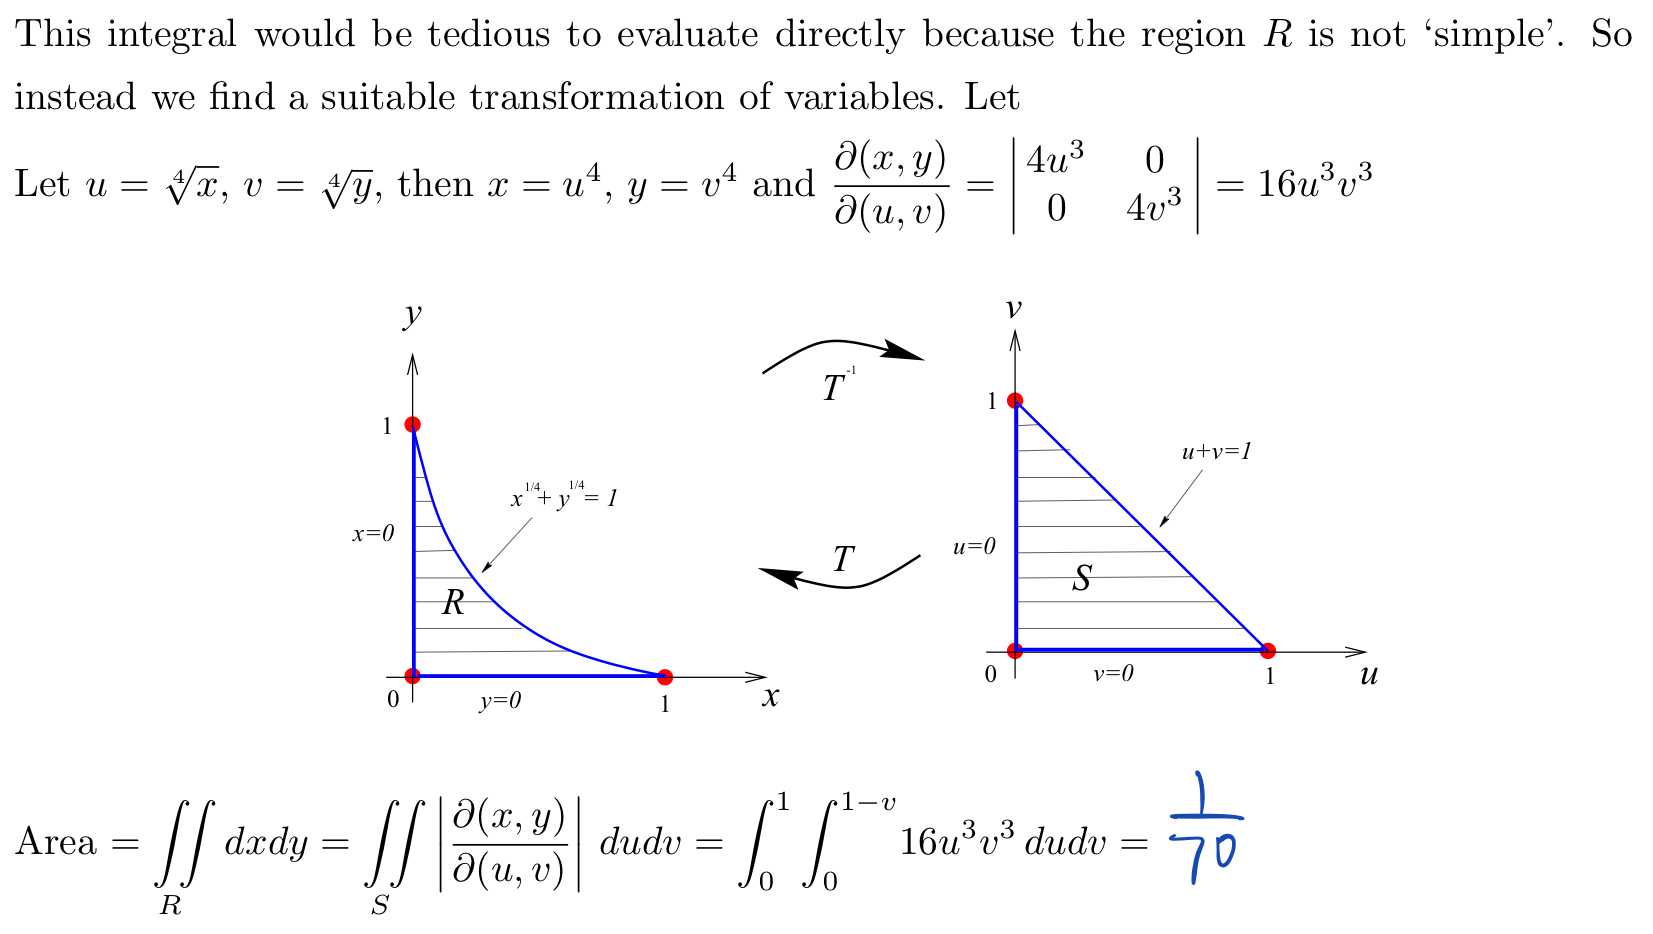
\includegraphics[scale=0.28]{images/Ch14-jacobian-eg2.jpeg}


    \newpage
    Sometimes, it's not easy to calculate $\dfrac{\partial(x, y)}{\partial(u, v)}$, 
    since usually we substitute $u$ and $v$ as functions of $x$ and $y$, so we always need to find the inverse 
    function in order to calculate $\dfrac{\partial(x, y)}{\partial(u, v)}$. So we consider the relationship 
    between  $\dfrac{\partial(x, y)}{\partial(u, v)}$ and $\dfrac{\partial(u, v)}{\partial(x, y)}$.

    Because of $\det A \det B=\det(AB)$, 
    \begin{align*}
        \frac{\partial(x, y)}{\partial(u, v)} \cdot \frac{\partial(u, v)}{\partial(x, y)} 
        &= \left|\begin{array}{ll}\frac{\partial x}{\partial u} & \frac{\partial x}{\partial v} \\ 
            \frac{\partial y}{\partial u} & \frac{\partial y}{\partial v}\end{array} \right| 
            \left|  \begin{array}{ll}\frac{\partial u}{\partial x} & \frac{\partial u}{\partial y} \\ 
                \frac{\partial v}{\partial x} & \frac{\partial v}{\partial y}\end{array}\right|\\
        &= \left|\begin{array}{ll}\frac{\partial x}{\partial u} \frac{\partial u}{\partial x}+\frac{\partial x}{\partial v} \frac{\partial v}{\partial x} & 
            \frac{\partial x}{\partial u} \frac{\partial u}{\partial y}+\frac{\partial x}{\partial v} \frac{\partial v}{\partial y} \\ 
            \frac{\partial y}{\partial u} \frac{\partial u}{\partial x}+\frac{\partial y}{\partial v} \frac{\partial v}{\partial x} & 
            \frac{\partial y}{\partial u} \frac{\partial u}{\partial y}+\frac{\partial y}{\partial v} \frac{\partial v}{\partial y}\end{array}\right| \\ 
        &=\left|\begin{array}{ll}\frac{\partial x}{\partial x} & \frac{\partial x}{\partial y} \\ 
                \frac{\partial y}{\partial x} & \frac{\partial y}{\partial y}\end{array}\right|
        =\left|\begin{array}{cc}1 & 0 \\ 0 & 1\end{array}\right|=1
    \end{align*}

    Therefore, if $x(u,v)$ and $y(u,v)$ have continuous first partial derivatives, and that 
    $$\frac{\partial(x, y)}{\partial(u, v)} \neq 0 \quad \text { at } \quad(u, v) \quad \text { (one-to-one map). }$$
    Then
    \begin{center}
        \boxed{$$\disp \frac{\partial(x, y)}{\partial(u, v)}=\frac{1}{\dfrac{\partial(u, v)}{\partial(x, y)}}$$}
    \end{center}

    \newpage
    {\blue This example shows the situation when $\dfrac{\partial(x, y)}{\partial(u, v)}$ is difficult to compute.}
    
    \eg Find $\disp \iint_{A}\left(x^{2}+y^{2}\right) d x d y$, 
    where $A=\left[(x, y) \mid x, y>0, \quad 2 \leqslant x^{2}-y^{2} \leqslant 4, \quad \frac{1}{2} \leqslant x y \leqslant \frac{3}{2}\right]$

    \sol 
    
    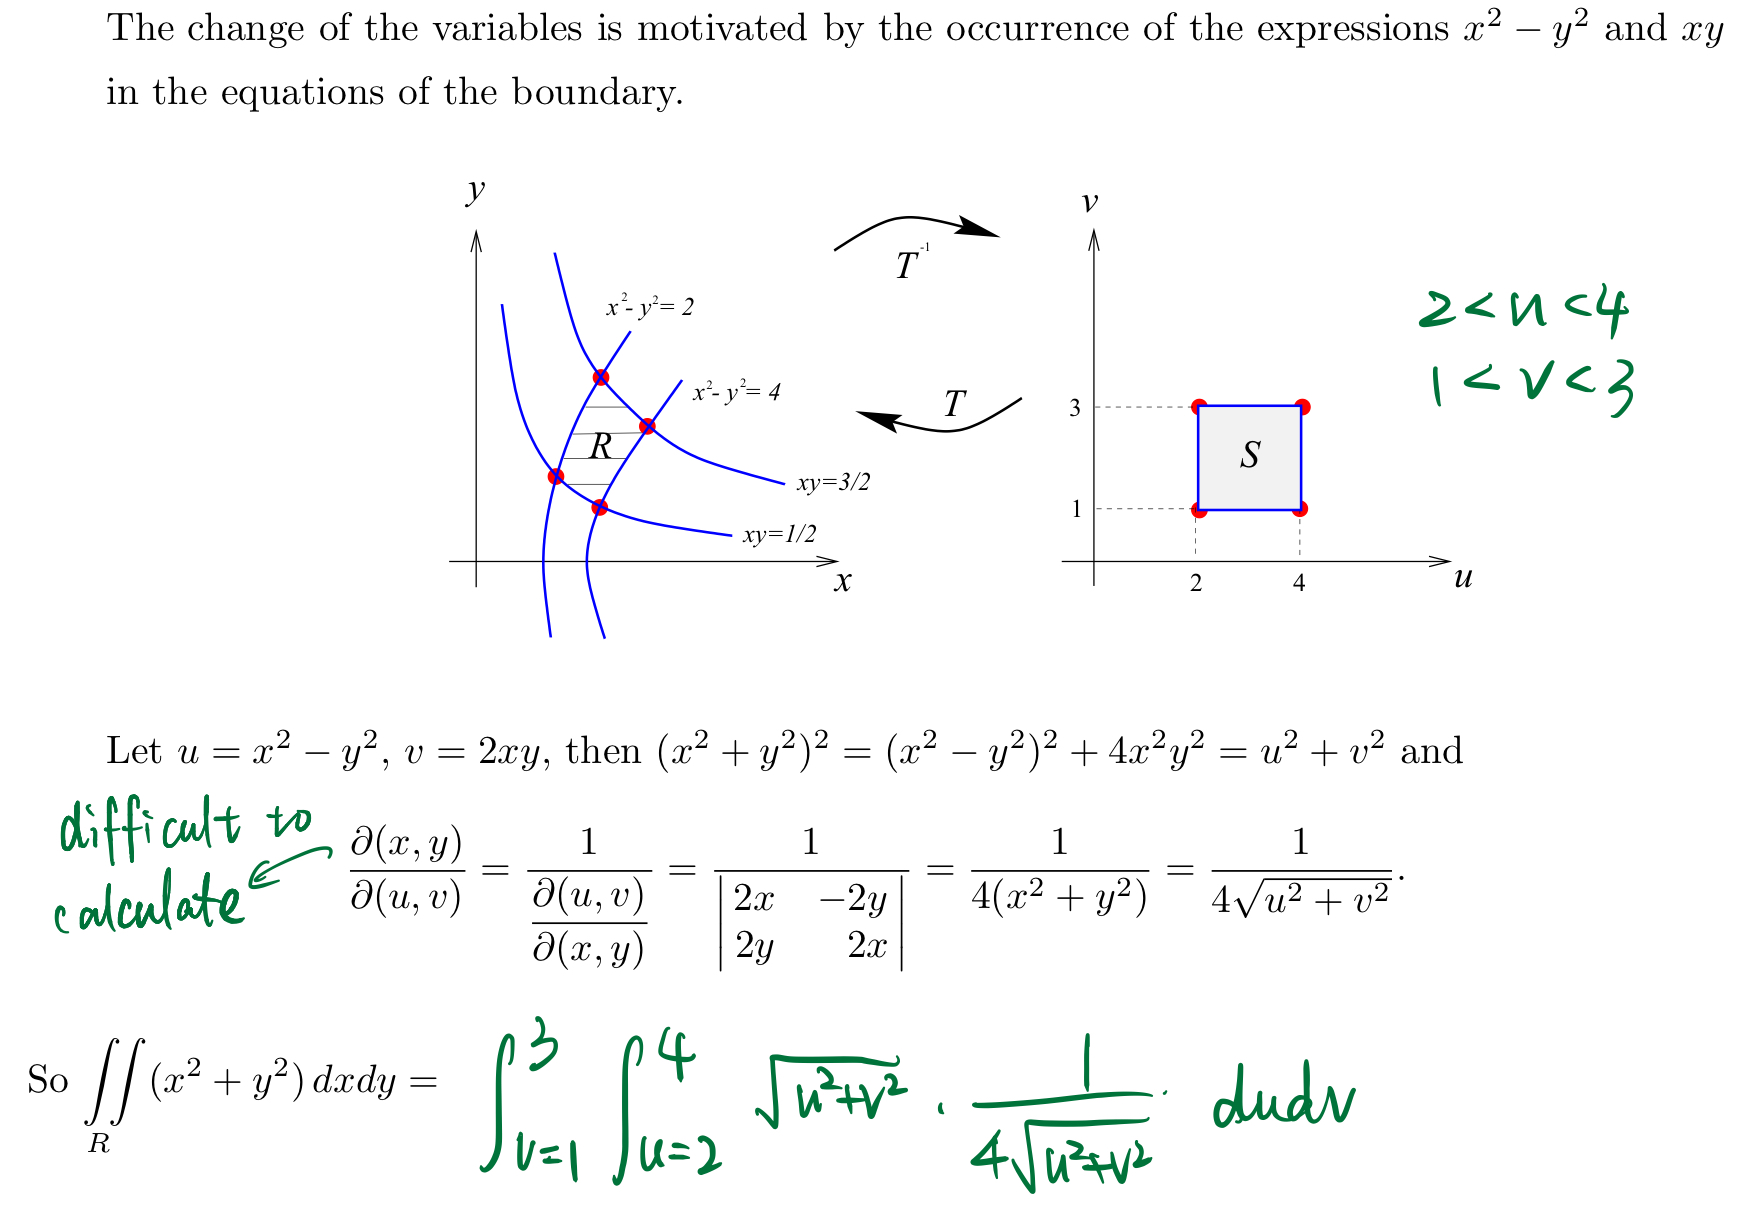
\includegraphics[scale=0.25]{images/Ch14-jacobian-eg3.jpeg}


    \newpage
    Sometimes, though the given region is a relatively good one, but it's still difficult to directly
    integrate, maybe because the integrand is too complicated. See the below example:

    \eg 
    
    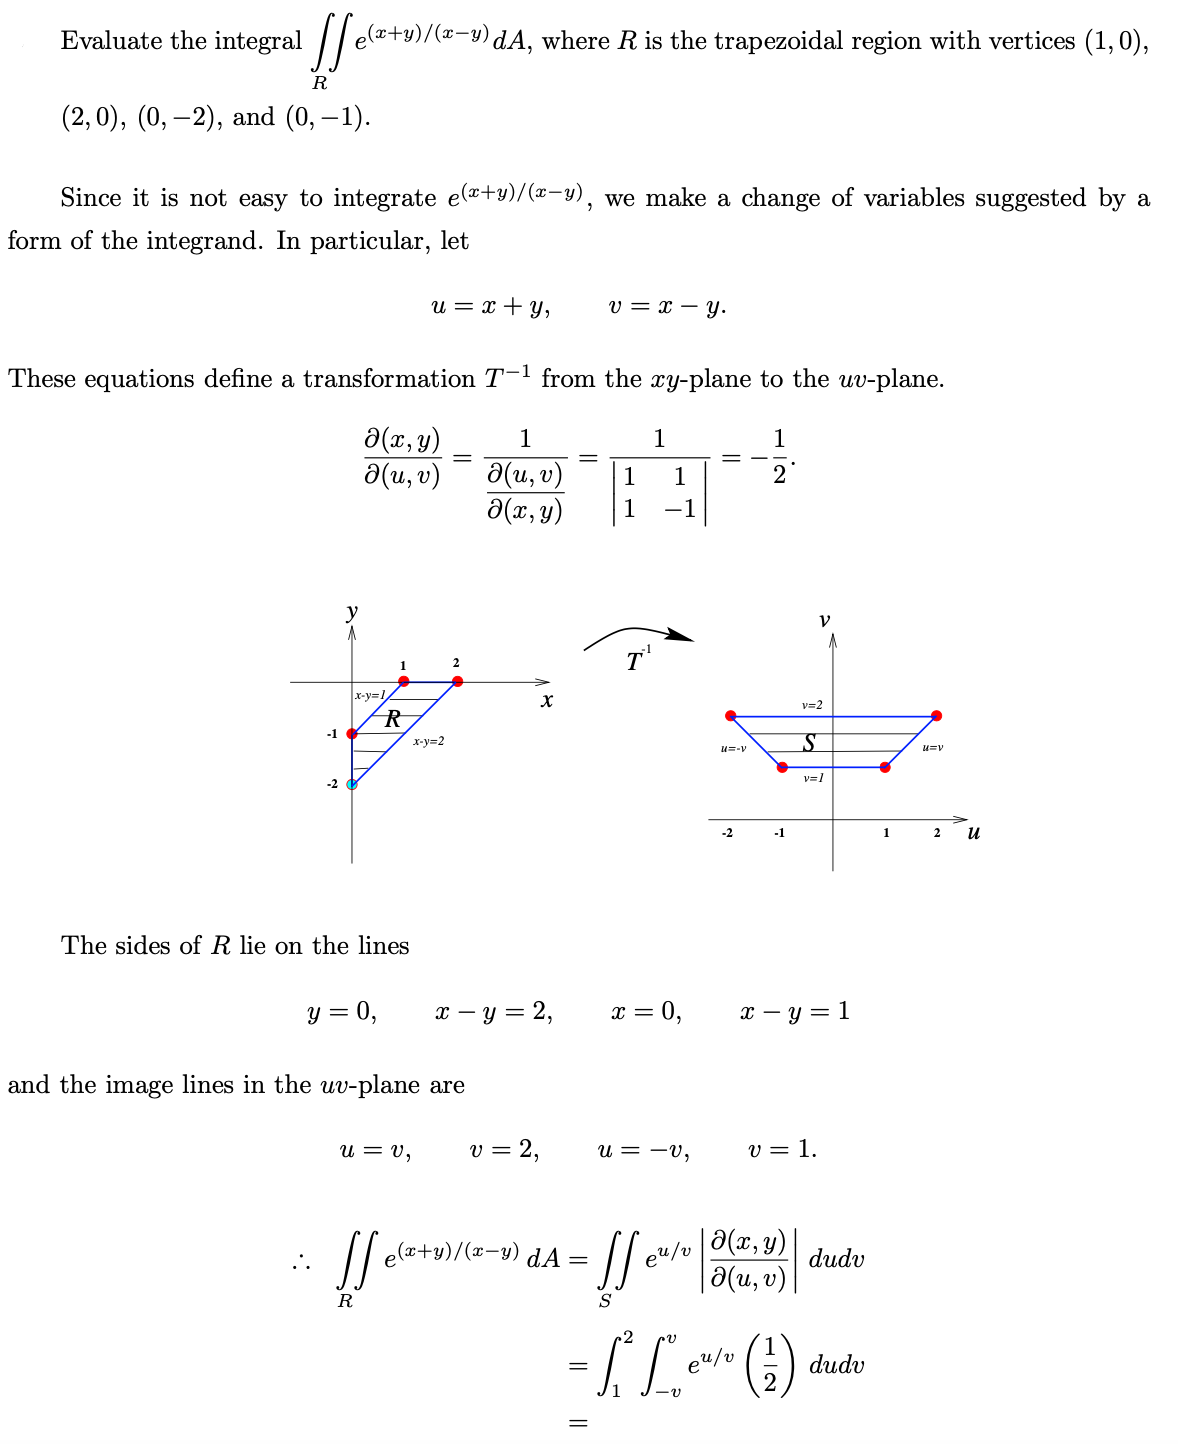
\includegraphics[scale=0.77]{images/Ch14-jacobian-eg4.png}


    \newpage
    \section{Triple Integrals in Cylindrical \& Spherical Coordinates}

    {\bf Cylindrical} coordinates are suited to problems {\it with axial symmetry}(the shape 
    is around the $z$-axis)

    The basic unit of cylindrical coordinate is shown below, and it's volume is $r\ drd\theta dz$
    \begin{center}
        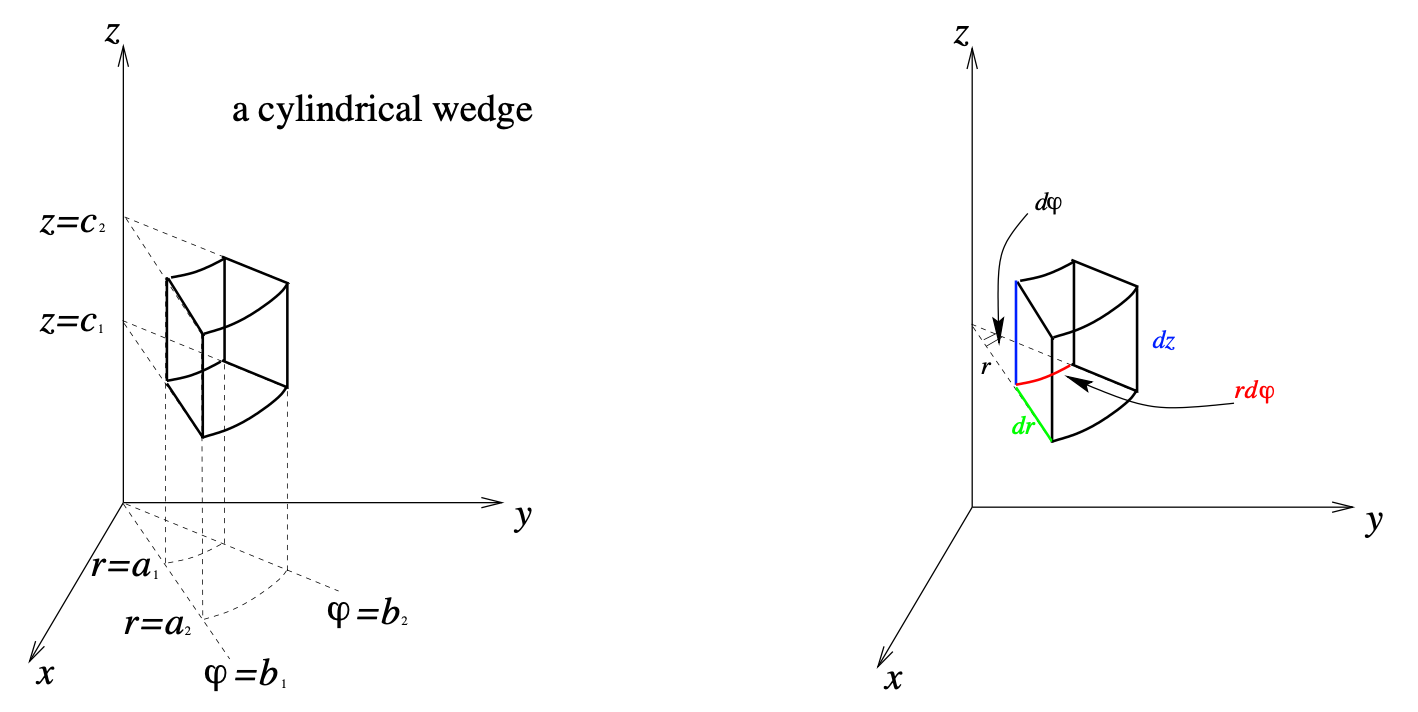
\includegraphics[scale=0.43]{images/Ch14-int-cylind.png}
    \end{center}
    We can also find Jacobian in order to find the relation. For $x=r\cos \theta, y=r\sin\theta,z=z$, we have
    $$\frac{\partial(x,y,z)}{\partial(r,\theta,z)}=
    \left|\begin{array}{ccc}
        \cos\theta & -r\sin\theta & 0\\
        \sin\theta & r\cos\theta & 0\\
        0 & 0 & 1
    \end{array}\right|=r$$
    that is, $dxdydz\rightarrow r\ drd\theta dz$

    \vspace{0.2in}
    \begin{center}
        \boxed{$$\disp V_{c}=\iiint_{V} f d V=\iiint_{V(x, y, z)} f(x, y, z) d x d y d z
        =\iiint_{V(r, \theta, z)} f(r, \theta, z) r d r d \theta d z$$}
    \end{center}

    \newpage
    Moreover, same as before, we can freely change the {\it order of integration}.
    Below show three examples.
    \begin{center}
        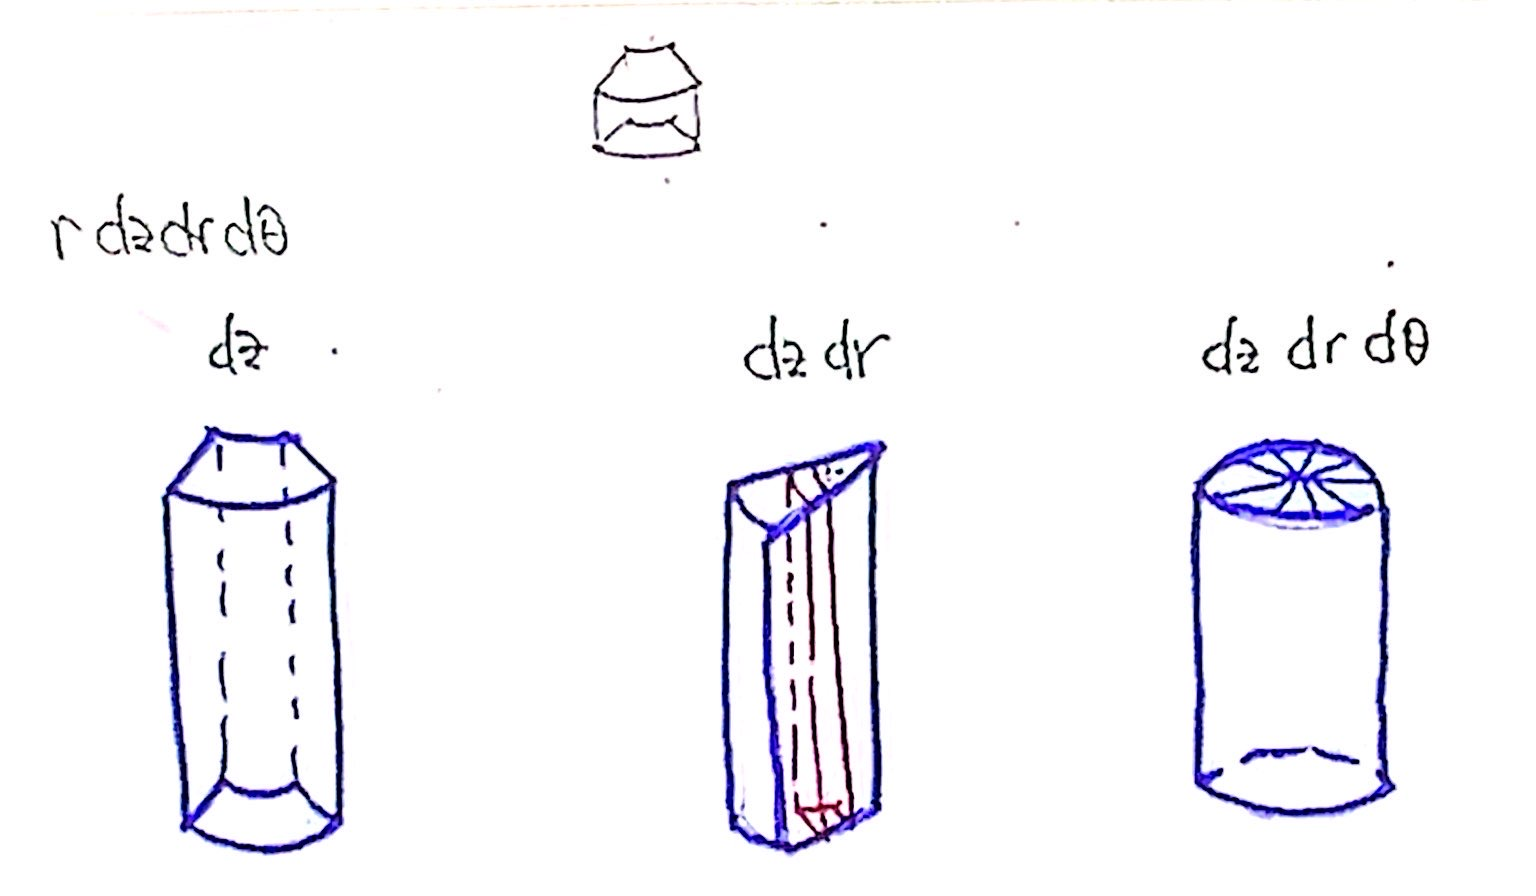
\includegraphics[scale=0.20]{images/Ch14-int-cylind-ways-1.JPG}

        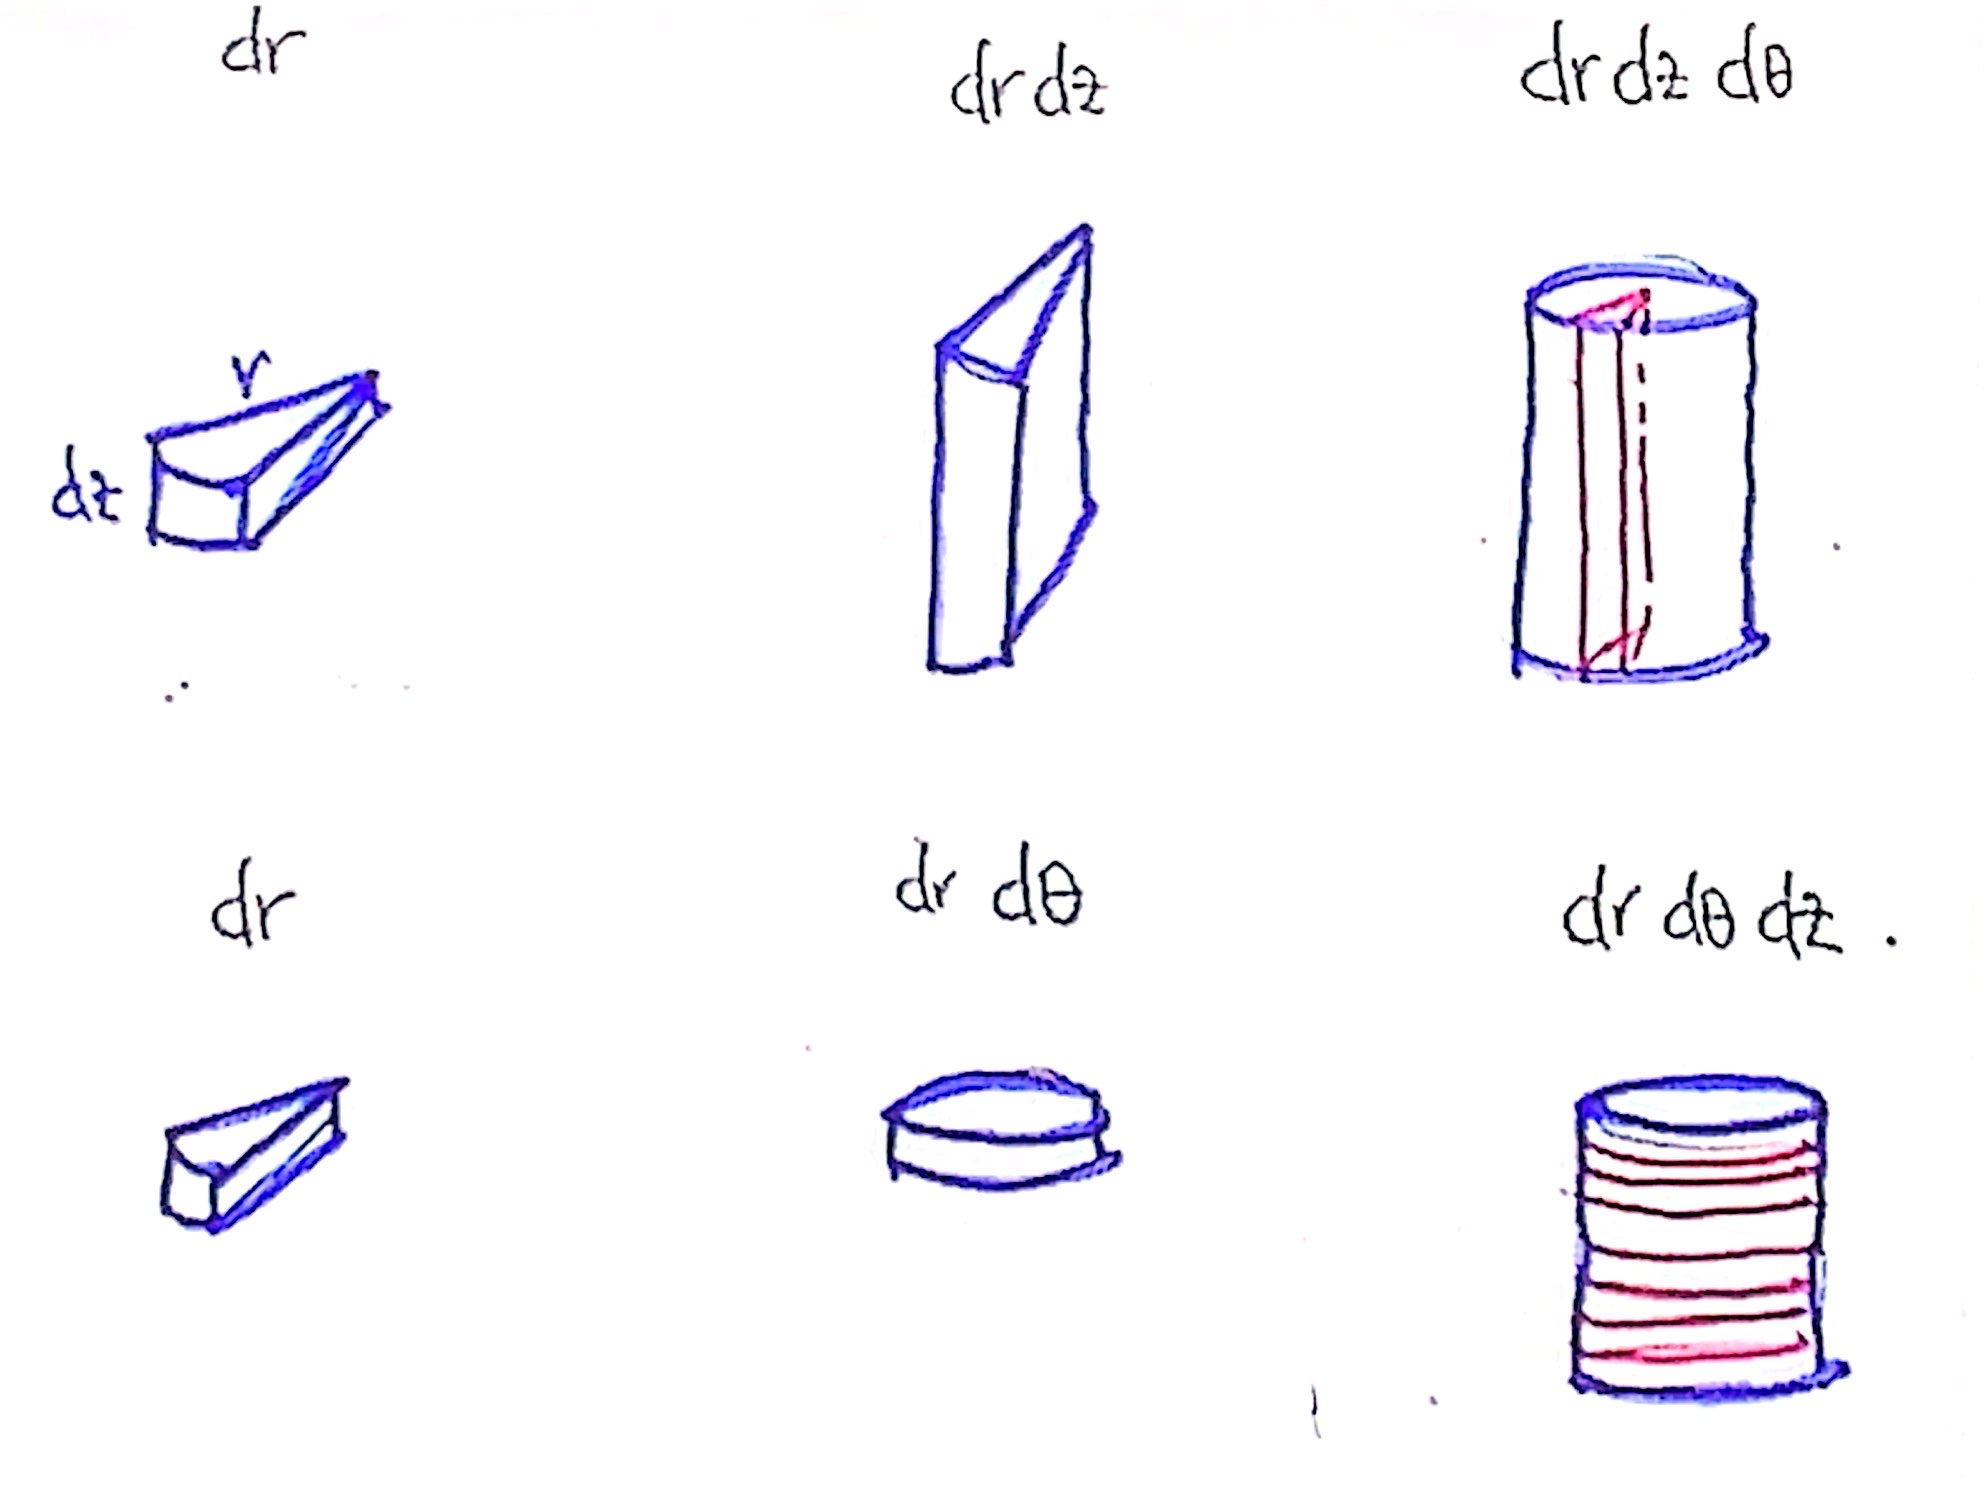
\includegraphics[scale=0.17]{images/Ch14-int-cylind-ways-2.JPG}
    \end{center}

    \newpage
    {\blue This example shows integration in cylindrical coordinates brings convenience sometimes.}

    \eg Find the volume of a circular cone with altitude $h$ and a base of radius $a$.
    
    \sol To find the volume of the cone, we need to know the equation of its surface.

    \begin{center}
        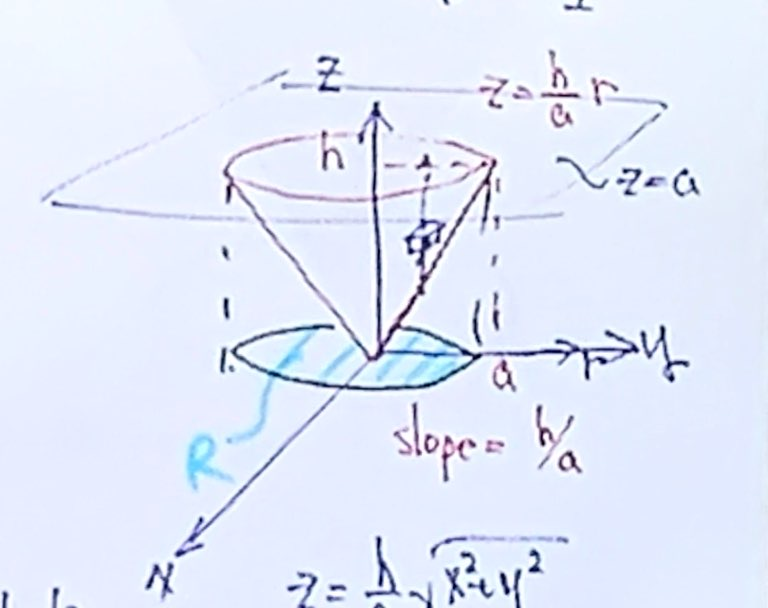
\includegraphics[scale=0.25]{images/Ch14-int-cylind-eg1.JPG}
    \end{center}

    In $(x,y,z), \disp z=\frac{h}{a}(x^2+y^2)^{1/2}$. \quad 
    In $\disp (r,\theta,z), z=\frac{h}{a}r$.

    {\bf Method 1:} Do the question by $(x,y,z)$, and $dV=dzdydx$
    $$V=4\int_{0}^a\int_0^{\sqrt{a^2-x^2}}\int_{\frac{h}{a}(x^2+y^2)^{1/2}}^{h}\ dz\ dy\ dx$$

    {\bf Method 2:} Do the question by $(r,\theta,z)$, and $dV=r\ dzdrd\theta$
    $$V=\int_0^{2\pi} \int_0^a \int_{\frac{h}{a}r}^h\ r\ dz\ dr\ d\theta=\dfrac{1}{3}\pi a^2h$$

    \newpage
    {\blue This example provides interpretation for triple integrals.}

    \eg Sketch the solid whose volume is given by the integral.

    (a) $\disp \int_0^{2\pi} \int_0^2 \int_0^{4-r^2}\ r\ dzdrd\theta$.

    (b) $\disp \int_1^3 \int_0^{\frac{\pi}{2}} \int_r^3\ r\ dzd\theta dr$.

    \sol Recall that for $\disp \int_a^b \int_{g_1(x)}^{g_2(x)} \int_{\phi_1(x)}^{\phi_2(x)}\ dzdydx$,
    we can infer the volume of integration based on these six limits: 

    $z=\phi_1$ to $z=\phi_2$, (surfaces)\\
    $y=g_1$ to $y=g_2$, (curves)\\
    $x=a$ to $x=b$, (points)

    We can interpret the last two as ``{\it area on the $xy$-plane}''.
    
    (a)

    $z: z=0$ to $z=4-r^2$, (surfaces)

    $\left.\begin{array}{ccc}
        r: r=0 & {\rm to} & r=2\\
        \theta: \theta=0 & {\rm to} & \theta = 2\pi 
    \end{array}\right\}$  (area on $xy$-plane)

    The area on $xy$-plane is shown below left. We move the disk upward, hitting $z=4-r^2$, 
    and the volume bounded is what we are looking for, as shown below right.
    \begin{center}
        
    \begin{tikzpicture}[x=0.75pt,y=0.75pt,yscale=-1,xscale=1]
    %uncomment if require: \path (0,221); %set diagram left start at 0, and has height of 221

    %Shape: Axis 2D [id:dp35767444761973244] 
    \draw  (26.67,96.18) -- (154.33,96.18)(89.22,32.33) -- (89.22,160) (147.33,91.18) -- (154.33,96.18) -- (147.33,101.18) (84.22,39.33) -- (89.22,32.33) -- (94.22,39.33)  ;
    %Shape: Circle [id:dp0770483128463828] 
    \draw  [fill={rgb, 255:red, 74; green, 144; blue, 226 }  ,fill opacity=0.54 ] (58.81,96.18) .. controls (58.81,79.38) and (72.42,65.76) .. (89.22,65.76) .. controls (106.02,65.76) and (119.64,79.38) .. (119.64,96.18) .. controls (119.64,112.98) and (106.02,126.6) .. (89.22,126.6) .. controls (72.42,126.6) and (58.81,112.98) .. (58.81,96.18) -- cycle ;

    % Text Node
    \draw (74.67,22.73) node [anchor=north west][inner sep=0.75pt]    {$y$};
    % Text Node
    \draw (155.33,87.4) node [anchor=north west][inner sep=0.75pt]    {$x$};
    % Text Node
    \draw (118.64,99.58) node [anchor=north west][inner sep=0.75pt]  [font=\small]  {$2$};
    % Text Node
    \draw (89.67,51.4) node [anchor=north west][inner sep=0.75pt]  [font=\small]  {$2$};
    % Text Node
    \draw (44,165.07) node [anchor=north west][inner sep=0.75pt]  [font=\small]  {$ \begin{array}{l}
    r=0\ to\ r=2\\
    \theta =0\ to\ \theta =2\pi 
    \end{array}$};
    \end{tikzpicture}
    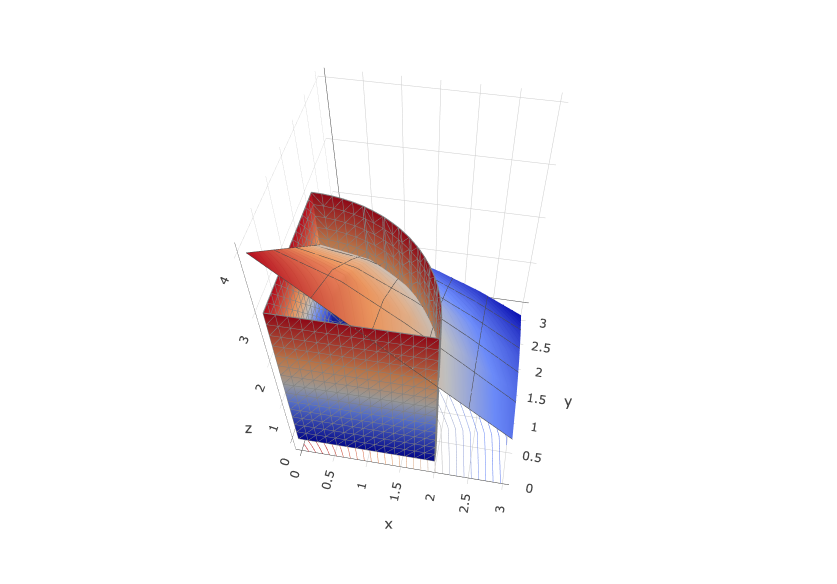
\includegraphics[scale=0.3]{images/Ch14-int-cylid-eg2-2.png}

    \end{center}

    \newpage
    (b)

    $z: z=r$ to $z=3$, (surfaces)

    $\left.\begin{array}{ccc}
        \theta: \theta=0 & {\rm to} & \theta = \frac{\pi}{2} \\
        r: r=1 & {\rm to} & r=3
    \end{array}\right\}$  (area on $xy$-plane)

    The procedure is similar to (a), we first draw the region on $xy$-plane, and 
    move it from surface $z=r$ upwards to $z=3$. The bounded region is what we're looking for.
    \begin{center}
        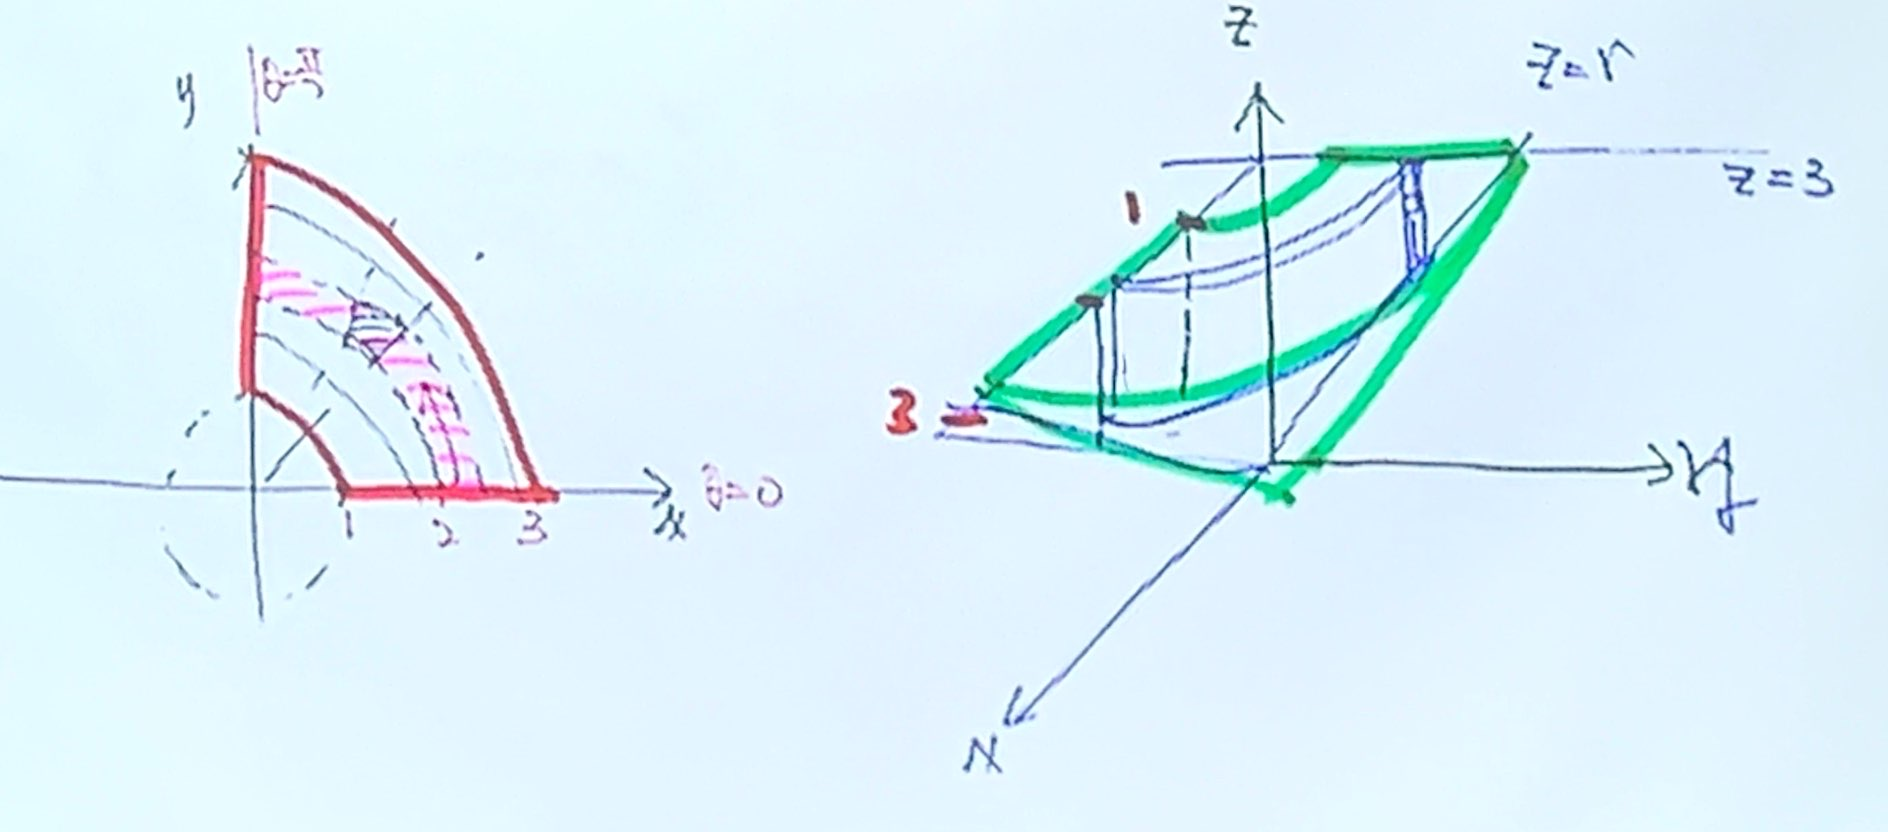
\includegraphics[scale=0.16]{images/Ch14-int-cylind-eg3-1.JPG}
        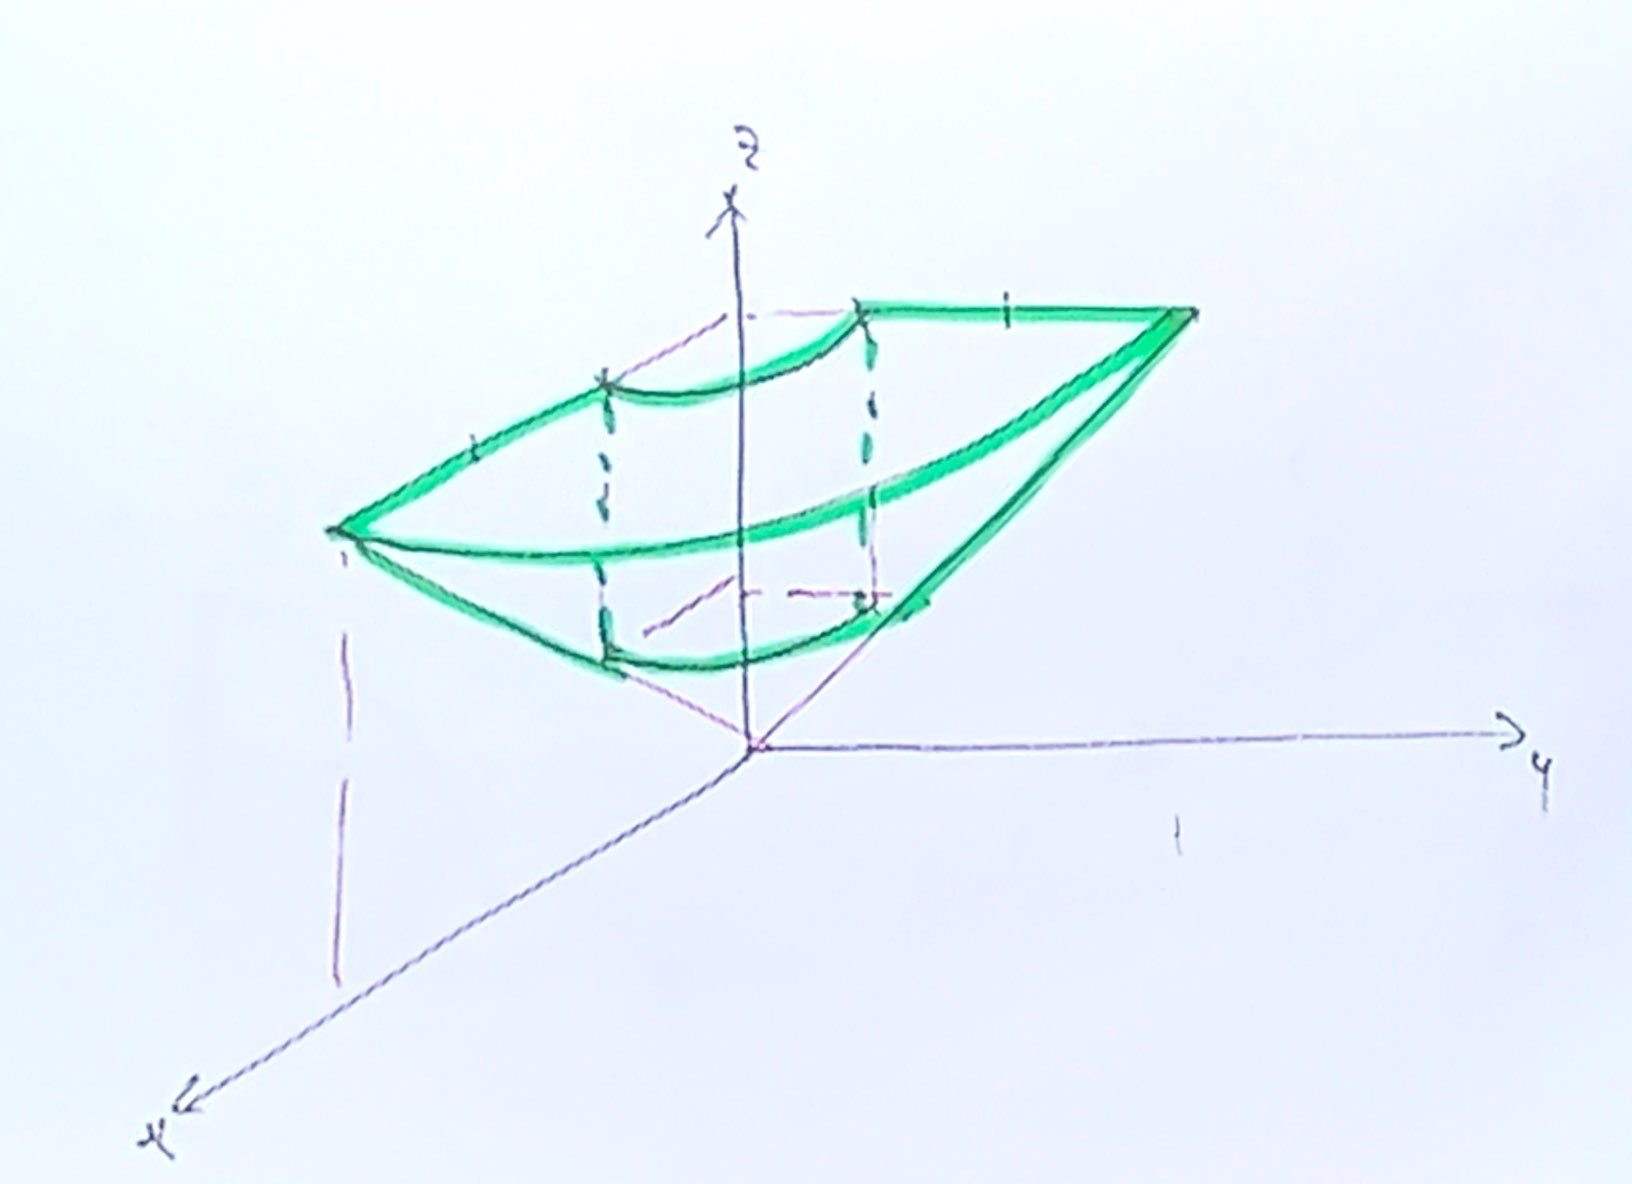
\includegraphics[scale=0.1]{images/Ch14-int-cylind-eg3-2.JPG}
    \end{center}
    

    \newpage
    {\bf Spherical} coordinates are suited to problems {\it involving spherical symmetry}, 
    and in particular, to regions bounded by {\it spheres} centered at the origin, {\it circular 
    cones} with axes along the $z-$axis, {\it vertical planes} containing $z-$axis.

    The basic unit of spherical coordinate is shown below, and it's volume is 
    $dV=\rho^2 \sin\phi \ d\theta d\rho d\phi$
    \begin{center}
        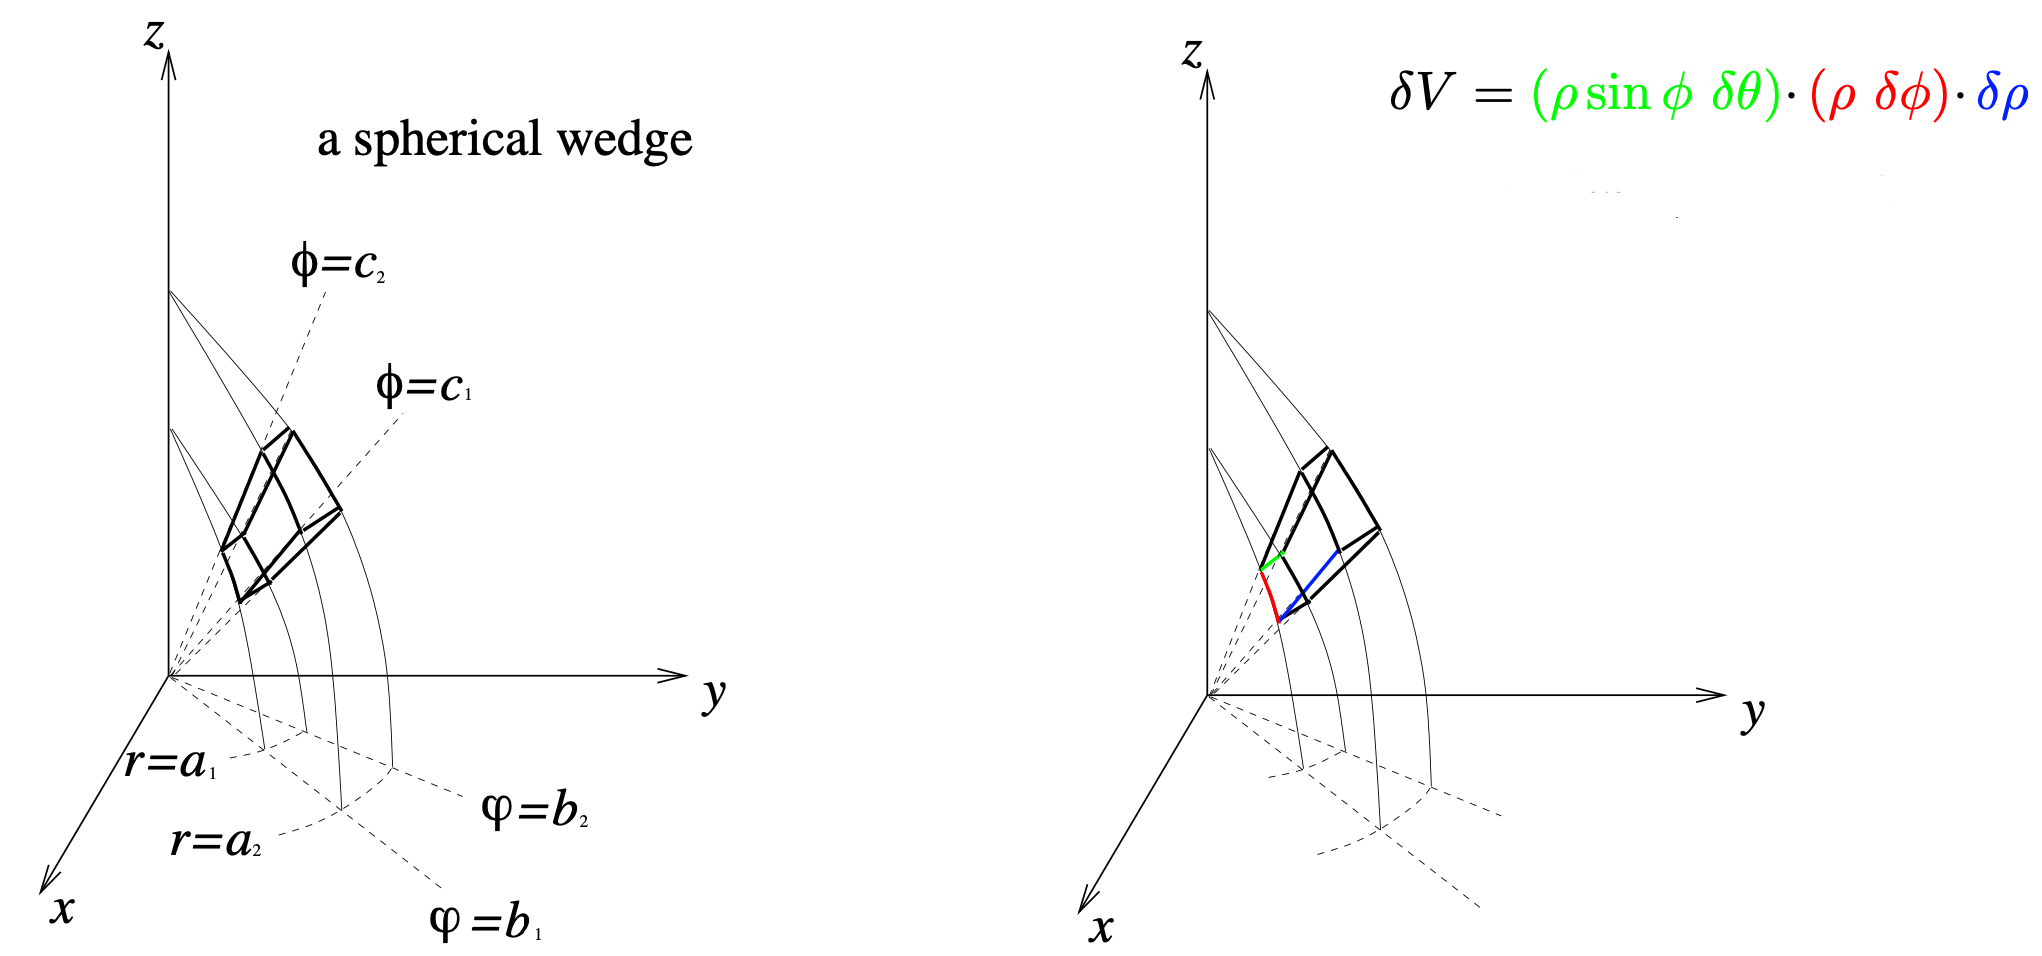
\includegraphics[scale=0.35]{images/Ch14-int-sphere-1.png}
        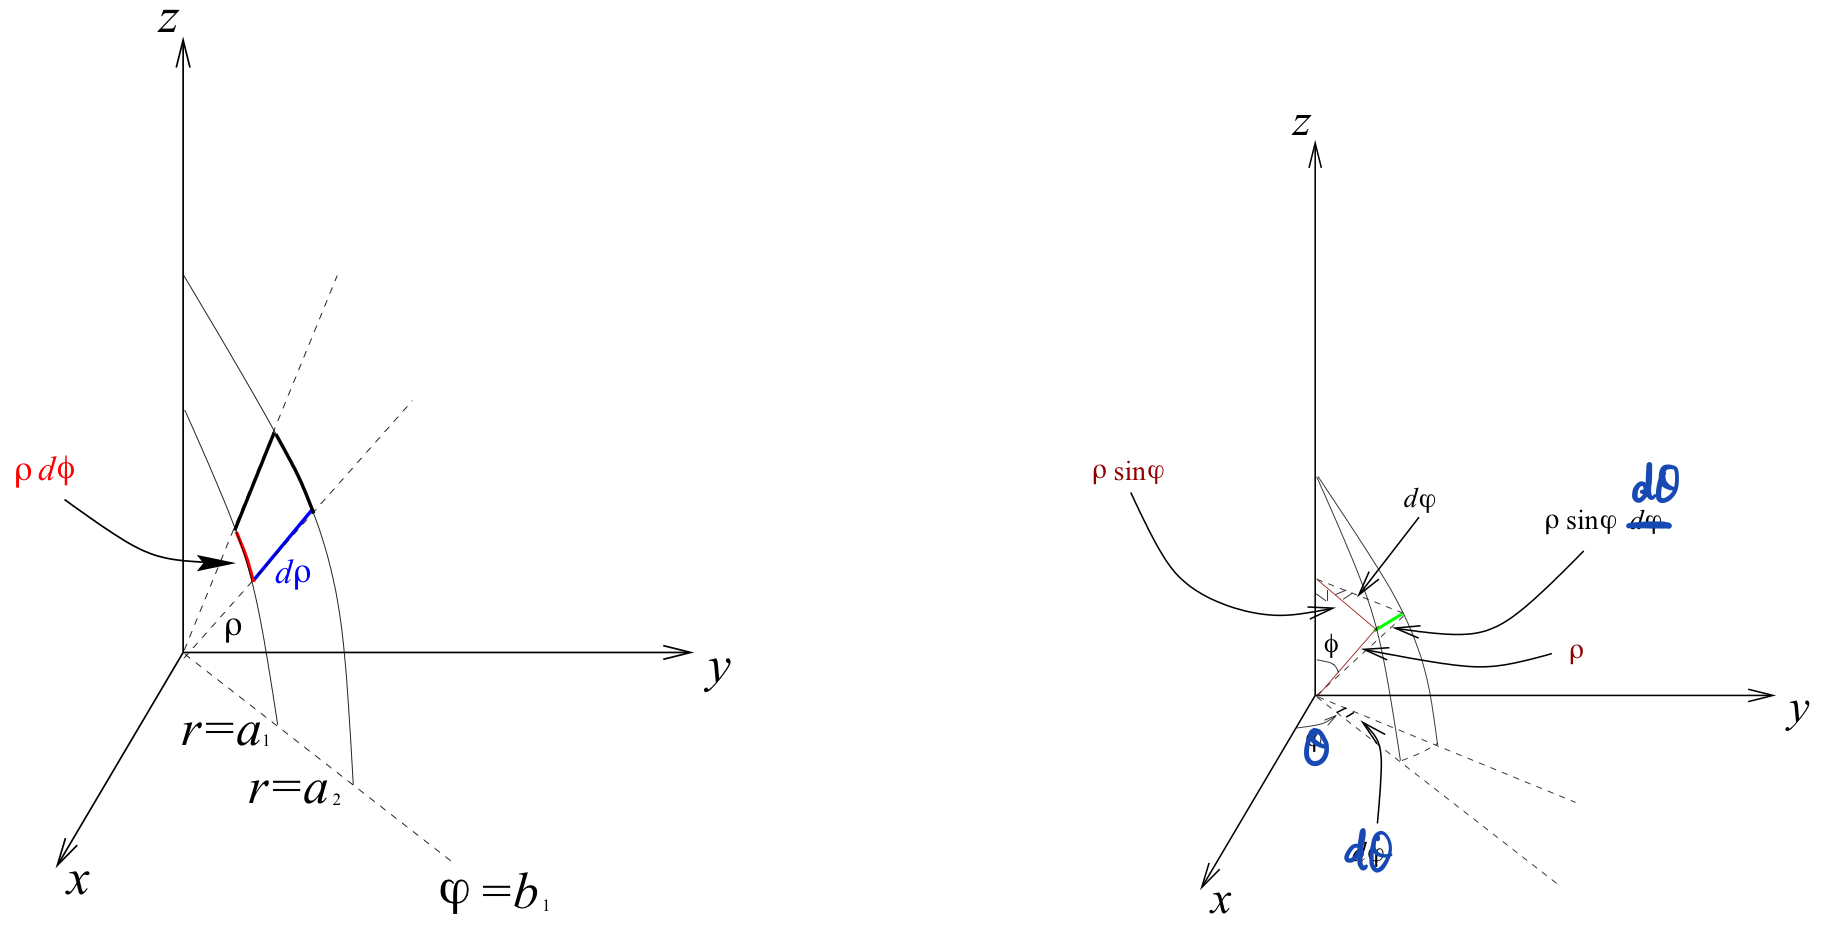
\includegraphics[scale=0.2]{images/Ch14-int-sphere-2.jpeg}
    \end{center}
    We can also find Jacobian in order to find the relation. 

    For spherical coordinates $x=\rho \sin \phi \cos \theta, y=\rho \sin \phi \sin \theta$ and $z=\rho \cos \phi$, then
    $$
    \frac{\partial(x, y, z)}{\partial(\rho, \phi, \theta)}=\left|\begin{array}{ccc}
    \sin \phi \cos \theta & \rho \cos \phi \cos \theta & -\rho \sin \phi \sin \theta \\
    \sin \phi \sin \theta & \rho \cos \phi \sin \theta & \rho \sin \phi \cos \theta \\
    \cos \phi & -\rho \sin \phi & 0
    \end{array}\right|=\rho^{2} \sin \phi
    $$
    i.e. $d x d y d z=\rho^{2} \sin \phi d \rho d \theta d \phi$.

    \vspace{0.5in}
    Again, different integration orders have different interpretations.

    \begin{center}
        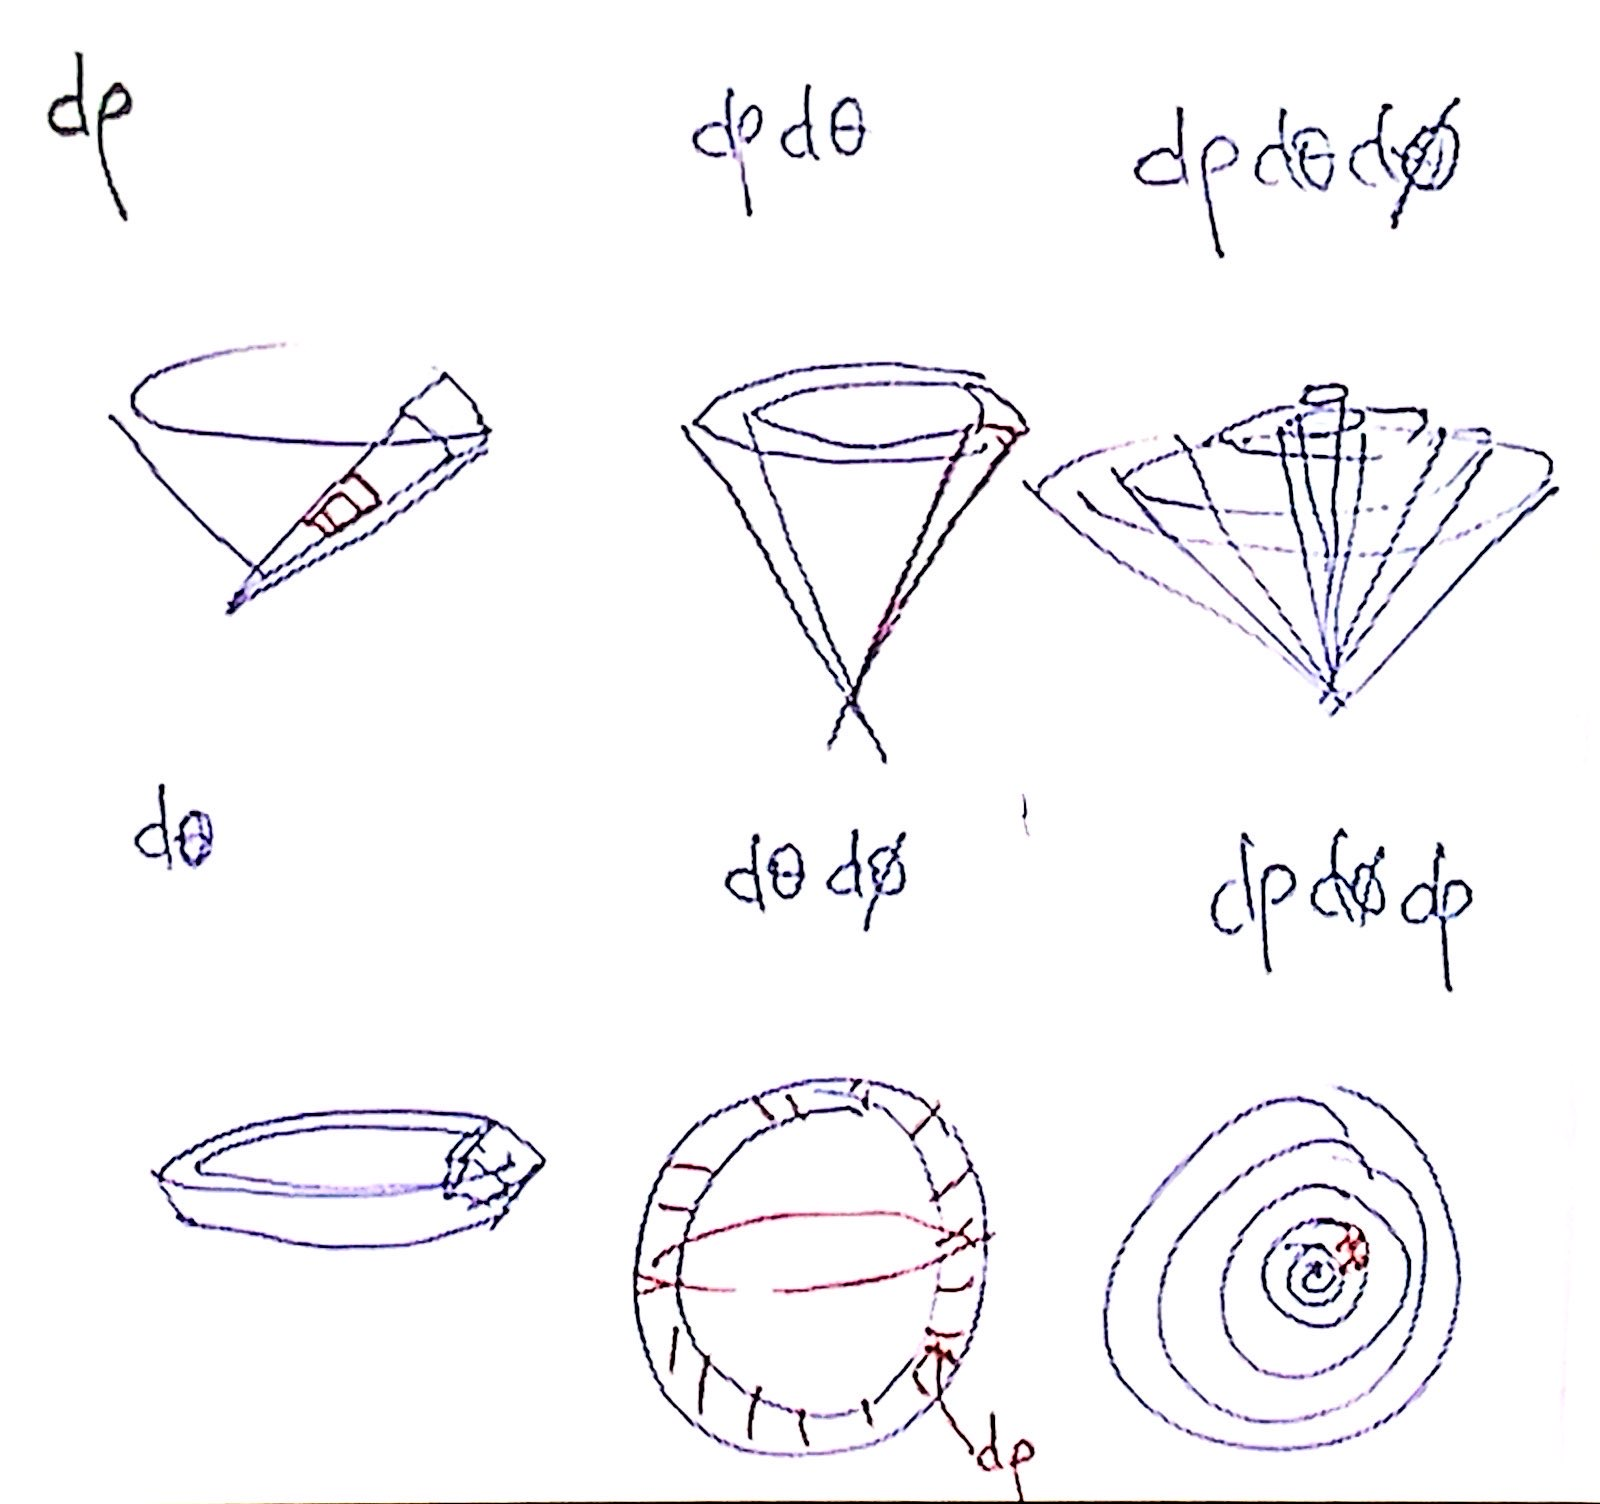
\includegraphics[scale=0.2]{images/Ch14-int-sphere-ways.JPG}
    \end{center}

    \newpage
    {\blue This example shows the choice of coordinate system can greatly affect the difficulty of 
    computation of a multiple integral.}

    \eg Find the volume of the solid that lies above the cone $z=\sqrt{x^2+y^2}$ and between the 
    sphere $x^2+y^2+z^2=z$.

    \sol The equation of sphere can be written as 
    $$x^{2}+y^{2}+\left(z-\frac{1}{2}\right)^{2}=\left(\frac{1}{2}\right)^{2} 
    \Rightarrow {\rm centre} \left(0,0, \frac{1}{2}\right),\ {\rm radius} =\frac{1}{2}$$

    {\bf Method 1:} Use Cartesian Coordinate: 
    \begin{center}
        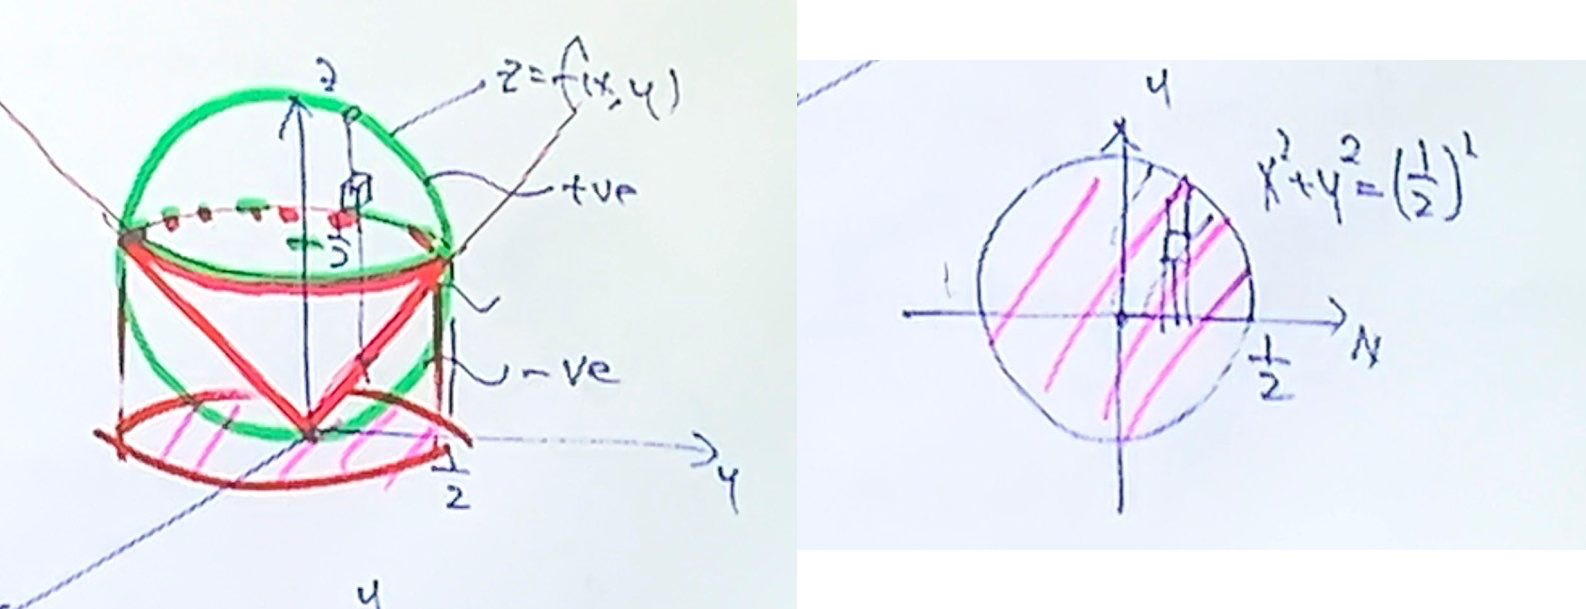
\includegraphics[scale=0.25]{images/Ch14-ex6.10-xy.jpg}
    \end{center}
    
    {\bf Cone:} $z=\sqrt{x^2+y^2}$\\
    {\bf Sphere:} $\disp z=\frac{1}{2}+\sqrt{\frac{1}{4}-x^2-y^2}$

    $$V=4\int_0^{\frac{1}{2}}\int_0^{\sqrt{\frac{1}{4}-x^2}} \int_{\sqrt{x^2+y^2}}^{\frac{1}{2}+\sqrt{\frac{1}{4}-x^2-y^2}}
    \ dzdydx$$

    {\bf Method 2:} Use Cylindrical Coordinate: 
    \begin{center}
        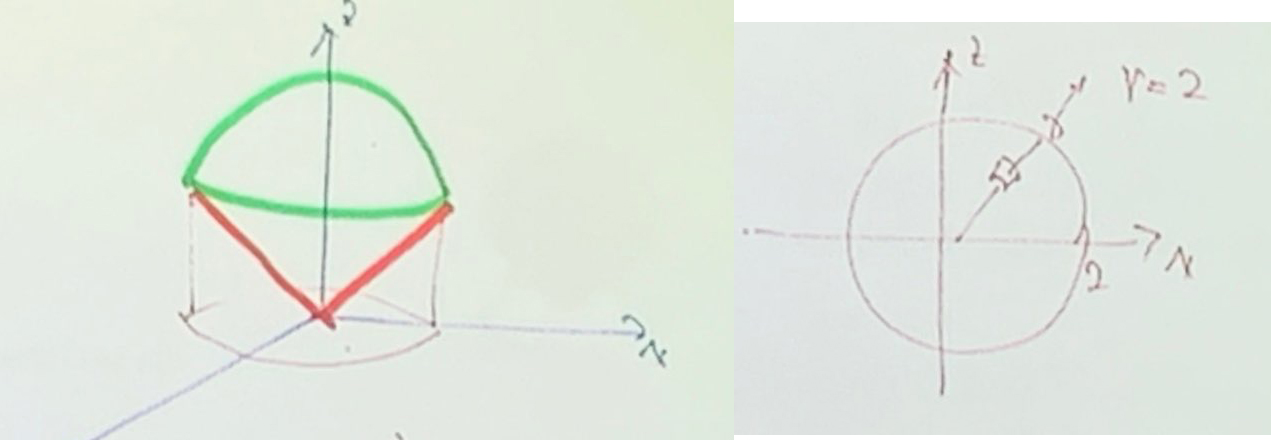
\includegraphics[scale=0.3]{images/Ch14-ex6.10-cylind.jpg}
    \end{center}
    
    {\bf Cone:} $z=\sqrt{x^2+y^2}=r$\\
    {\bf Sphere:} $\disp z=\frac{1}{2}+\sqrt{\frac{1}{4}-x^2-y^2}=\frac{1}{2}+\sqrt{\frac{1}{4}-r^2}$

    $$V=\int_0^{2\pi} \int_0^2 \int_r^{\frac{1}{2}+\sqrt{\frac{1}{4}-r^2}}\ r\ dzdrd\theta$$

    {\bf Method 3:} Use Spherical Coordinate: 
    \begin{center}
        \includegraphics[scale=0.28]{images/Ch14-ex6.10-sphere.JPG}
    \end{center}
    
    {\bf Cone:} $z=\sqrt{x^2+y^2}=\rho \sin\phi$\\
    {\bf Sphere:} $x^2+y^2+z^2=z \Rightarrow \rho^2 = \rho \cos\phi \Rightarrow \rho=\cos\phi$, (since $\rho\ne 0$)

    $$dV=\int_0^{\frac{\pi}{4}} \int_0^{2\pi} \int_0^{\cos\phi}\ \rho^2 \sin\phi \ d\rho d\theta d\phi$$

    \newpage
    {\blue This example shows the situation when we need to integrate two parts.}

    \eg Find the volume of a cylinder with radius $a$ and height $h$.

    \sol {\bf Method 1:} Use Cylindrical Coordinate: 
    $$V=\int_0^{2\pi} \int_0^a \int_0^h\ r\ dzdrd\theta$$

    This is really simple by cylindrical coordinate, but things become different when using spherical.

    {\bf Method 2:} Use Spherical Coordinate: 

    Notice that for different $\phi$, the $\rho$ is bounded by two different equations.
    So we cannot do it in one integration, instead, we need to separate these two situations.
    \begin{center}
        \includegraphics[scale=0.25]{images/Ch14-int-sphere-cylinder.JPG}
    \end{center}
    For the above cone, the upper red surface is $z=h\Rightarrow \rho\cos\phi=h\Rightarrow \rho=h/{\cos\phi}$,
    $$V_1=\int_0^{\phi'}\int_0^{2\pi}\int_0^{\frac{h}{\cos\phi}}\ \rho^2\sin\phi\ d\rho d\theta d\phi$$

    For the bottom part, $\rho$ moves along the green line, from 0 to $x^2+y^2=a^2\Rightarrow \rho\sin\phi=a$,
    $$V_2=\int_{\phi'}^{\frac{\pi}{2}} \int_0^{2\pi} \int_0^{\frac{a}{\sin\phi}}\ \rho^2\sin\phi\ d\rho d\theta d\phi$$


    For the bolded black line(the threshold), $\disp \tan\phi'=\frac{a}{h}\Rightarrow \phi=\tan^{-1}\frac{a}{h}$.

    $$V=V_1+V_2$$




    

    


    \newpage
    \section{Surface Area}
    
    We now want to find the area of a surface. Finding an area on $xy$-plane is relatively easy, as we 
    have discussed early this chapter, but things become much more complicated when we are focusing
    on an arbitrary surface. So, we think about {\it projecting the area onto xy-plane}.

    \begin{center}
        \includegraphics[scale=0.24]{images/Ch14-surface-area.jpeg}
    \end{center}

    As shown above, we want to find the area of region $S$ in a surface. The first thing to do 
    is to project it onto $xy$-plane, resulting in a region $R$.

    As usual, we use small rectangles to cover region $R$, as the green rectangle shown above,
    assume two sides are $\Delta x$ and $\Delta y$, so the area of green rectangle is $\Delta A
    =\Delta x\Delta y$.

    Then we project the rectangle up to the surface $S$, resulting in a ``curved-parallelogram''
    surface, shown as red area in left-below image. To find this area, we know as long as 
    $\Delta x$ and $\Delta y$ are small enough, the black parallelogram formed by $\Delta x$ and $\Delta y$
    is a good approximation for that area. By the way, the area of parallelogram is ${\bf u}\times {\bf v}$.

    How to represent ${\bf u}$ and ${\bf v}$? See the right-below image, the slope of vector ${\bf u}$
    is $\disp f_x=\dfrac{\Delta z}{\Delta x}$, so the width of ${\bf u}$ is $\Delta x$ and the height 
    of ${\bf u}$ is $\Delta z = \Delta x\cdot f_x$.(Notice this image is graphed vertically, i.e., 
    in $xz$-plane)


    \begin{center}
        \includegraphics[scale=0.27]{images/Ch14-surface-area-vector.jpeg}
        \hspace{0.5in}
        \begin{tikzpicture}[x=0.75pt,y=0.75pt,yscale=-1,xscale=1]
        %uncomment if require: \path (0,300); %set diagram left start at 0, and has height of 300

        %Shape: Rectangle [id:dp4999523728151394] 
        \draw  [dash pattern={on 4.5pt off 4.5pt}] (198,115.33) -- (243.67,115.33) -- (243.67,206.01) -- (198,206.01) -- cycle ;
        %Straight Lines [id:da4188949615125863] 
        \draw  [dash pattern={on 4.5pt off 4.5pt}]  (243.67,115.33) -- (243.67,90.67) ;
        %Curve Lines [id:da0065392042697955954] 
        \draw    (198,115.33) .. controls (217.67,89.34) and (231,92.67) .. (243.67,90.67) ;
        %Straight Lines [id:da5679442967275912] 
        \draw [color={rgb, 255:red, 65; green, 117; blue, 5 }  ,draw opacity=1 ]   (198,115.33) -- (222.52,80.31) ;
        \draw [shift={(223.67,78.67)}, rotate = 485] [color={rgb, 255:red, 65; green, 117; blue, 5 }  ,draw opacity=1 ][line width=0.75]    (10.93,-3.29) .. controls (6.95,-1.4) and (3.31,-0.3) .. (0,0) .. controls (3.31,0.3) and (6.95,1.4) .. (10.93,3.29)   ;
        %Shape: Axis 2D [id:dp1593594891661796] 
        \draw  (150,202.67) -- (169,202.67)(151.9,178.67) -- (151.9,205.33) (162,197.67) -- (169,202.67) -- (162,207.67) (146.9,185.67) -- (151.9,178.67) -- (156.9,185.67)  ;

        % Text Node
        \draw (209,205.07) node [anchor=north west][inner sep=0.75pt]  [font=\small]  {$\Delta x$};
        % Text Node
        \draw (245.33,97.4) node [anchor=north west][inner sep=0.75pt]  [font=\small]  {$\Delta z$};
        % Text Node
        \draw (210,114.07) node [anchor=north west][inner sep=0.75pt]  [font=\small]  {$\Delta x$};
        % Text Node
        \draw (196.67,78.73) node [anchor=north west][inner sep=0.75pt]  [color={rgb, 255:red, 65; green, 117; blue, 5 }  ,opacity=1 ]  {$\mathbf{u}$};
        % Text Node
        \draw (171.33,193.73) node [anchor=north west][inner sep=0.75pt]  [font=\small]  {$\mathbf{i}$};
        % Text Node
        \draw (147.33,159.73) node [anchor=north west][inner sep=0.75pt]  [font=\small]  {$\mathbf{k}$};
        \end{tikzpicture}

    \end{center}

    Therefore, ${\bf u}=\Delta x {\bf i}+0{\bf j}+\Delta x\cdot f_x{\bf k}$, 
    similarly, ${\bf v}=0 {\bf i}+\Delta y {\bf j}+\Delta y\cdot f_y{\bf k}$.
    Then $$||{\bf u\times v}||=||-\Delta x\Delta yf_x {\bf i}-\Delta x\Delta yf_y {\bf j}
    +\Delta x\Delta y {\bf k}||=\sqrt{(f_x)^2+(f_y)^2+1} \cdot \Delta x\Delta y$$

    When $\Delta x, \Delta y \rightarrow 0$, the area of $S$ is given by: 
    \begin{center}
        \boxed{$$\disp A=\iint_R \sqrt{(f_x)^2+(f_y)^2+1}\ dA$$}
    \end{center}
    

    \eg Given a plane $ax+by+cz=d$, where $a,b,c,d>0$. Find the area of the triangle bounded 
    by the intersections of the plane and axes.(As the red shaded area shown)

    \begin{center}
        \includegraphics[scale=0.25]{images/Ch14-surface-area-eg1.jpeg}
    \end{center}

    \sol The equation of surface $z=f(x,y)$ is given by $z=\dfrac{d-ax-by}{c}$.

    To find the red area, we first {\it project it onto $xy$-plane}, resulting in green area $R$.

    Thus the red area $$S=\iint_R\sqrt{1+f_x^2+f_y^2}\ dA_{xy}$$

    We know that $f_x=-\dfrac{a}{c},\ f_y=-\dfrac{b}{c}$, so 
    $\sqrt{1+f_x^2+f_y^2}=\dfrac{\sqrt{a^2+b^2+c^2}}{c}$, then
    \begin{align*}
        S &= \iint_R{\blue \dfrac{\sqrt{a^2+b^2+c^2}}{c}}\ dA_{xy}\\
          &= \dfrac{\sqrt{a^2+b^2+c^2}}{c}\cdot {\rm (area\ of\ R)}\\
          &= \dfrac{\sqrt{a^2+b^2+c^2}}{c}\cdot \frac{1}{2}\cdot \frac{d}{a}\cdot \frac{d}{b}\\
          &= \frac{d^2\sqrt{a^2+b^2+c^2}}{2abc}
    \end{align*}
    Notice the blue part is a constant.

    \newpage
    \eg Find the surface area of the cone $z=\dfrac{h}{a}r$ (in cylindrical coordinate).
    \begin{center}
        \includegraphics[scale=0.25]{images/Ch14-surface-area-eg2.jpeg}
    \end{center}

    \sol Project the cone onto $xy$-plane, resulting in red area $R$.

    The surface is given by $z=f(x,y)=\dfrac{h}{a}\sqrt{x^2+y^2}$

    Thus the green area $$S=\iint_R\sqrt{1+f_x^2+f_y^2}\ dA_{xy}$$

    We know that $f_x=\dfrac{h}{a}\cdot \dfrac{x}{\sqrt{x^2+y^2}},\ f_y=\dfrac{h}{a}\cdot \dfrac{y}{\sqrt{x^2+y^2}}$, so 
    $\sqrt{1+f_x^2+f_y^2}=1+\dfrac{h^2}{a^2}$, then

    \begin{align*}
        S &= \iint_R \sqrt{a+\frac{h^2}{a^2}}\ dA_{xy}\\ 
          &= \sqrt{a+\frac{h^2}{a^2}} \cdot {\rm (Area\ of\ circle\ with\ radius\ a)}\\
          &= \pi a\cdot \sqrt{a^2+h^2}
    \end{align*}

    \newpage
    \eg Find the area of the surface $z=x+y^2$ that lies above the triangle with vertices (0,0), (1,1)
    and (0,1).

    \sol 
    \begin{center}
        \includegraphics[scale=0.3]{images/Ch14-surface-area-eg3.jpeg}
    \end{center}


    \newpage
    {\blue This example uses substitution while evaluating integral.}

    \eg Find the surface of a sphere with radius $a$.
    \begin{center}
        \includegraphics[scale=0.25]{images/Ch14-surface-area-eg4.jpeg}
    \end{center}

    \sol Again, project $S$ onto $xy$-plane to get region $R$.

    The equation of surface is given by $z=f(x,y)=\sqrt{a^2-x^2-y^2}$,
    
    The green area: $$S=\iint_R\sqrt{1+f_x^2+f_y^2}\ dA_{xy}$$

    We know that $f_x=\dfrac{-x}{\sqrt{a^2-x^2-y^2}},\ f_y=\dfrac{-y}{\sqrt{a^2-x^2-y^2}}$, so 
    $\sqrt{1+f_x^2+f_y^2}=1+\dfrac{x^2+y^2}{a^2-x^2-y^2}$, then
    $$S = \iint_R \sqrt{1+\dfrac{x^2+y^2}{a^2-x^2-y^2}}\ dA_{xy}$$
    Notice this integration is too difficult to calculate, so we consider using {\it polar coordinate}
    to substitute, let $r^2=x^2+y^2$, $dA=r\ drd\theta$, then 
    $$S = \iint_R \sqrt{1+\dfrac{r^2}{a^2-r^2}}\ r\ drd\theta=2\pi a^2$$

\end{spacing}


\chapter{Chapter 15: Vector Field}


\begin{spacing}{1.3}

    \section{Intro. to Vector Field}

    So far, we have learned two kinds of functions involving vector: 
    \begin{itemize}
        \item ${\bf r}(t)=x(t){\bf i}+y(t){\bf j}+z(t){\bf k}$: for each $t$, provides a {\it position} vector 
        $<x(t), y(t), z(t)>$, so this is a (parametric) curve.
        \item $z=f({\bf r})=f(x_1,x_2,\cdots,x_n)$: for a given vector ${\rm r}$, this gives a real number,
        so this is a function of {\it several variables}. This is also a {\bf scalar field} since for 
        any point ${\bf r}$ in {\bf field}, it gives a scalar value. 
    \end{itemize}
    Now we are looking at {\bf vector-valued} function ${\bf F}$ of a vector ${\bf r}$, i.e., ${\bf F(r)}$.
    This is a {\bf vector field}, which means for any point ${\bf r}$ in {\bf field}, it gives a vector 
    ${\bf F(r)}$. 

    You can consider a world map showing the {\it speed} and {\it direction} of wind.
    
    \newpage
    \begin{center}
        \includegraphics[scale=0.14]{images/Ch15-wind.JPG}
    \end{center}

    You can see that in a 2D map(like above), if we put a vector on each point, the vector must have 
    same dimension as the map, i.e., all vectors must also be 2D vectors.
    $${\bf F(r)}=\left\{
        \begin{array}{lll}
            (F_1({\bf r}), F_2({\bf r})) & {\bf r}=(x,y) & {\blue 2D}\\
            (F_1({\bf r}), F_2({\bf r}), F_3({\bf r})) & {\bf r}=(x,y,z) & {\blue 3D}\\
            (F_1({\bf r}), F_2({\bf r}), \cdots, F_n({\bf r})) & {\bf r}=(x_1, x_2,\cdots, x_n) & {\blue nD}
        \end{array}\right.$$
    {\bf Summary:} {\it dimension of ${\bf F}$ must be the same as ${\bf r}$.}

    \vspace{0.3in}
    {\blue This is an example of vector field.}

    \eg Assume a vector field: ${\bf F}(x,y)=\dfrac{y\ii -x\jj}{\sqrt{x^2+y^2}}$.

    \sol Notice that $||{\bf F}||=\dfrac{y^2}{x^2+y^2}+\dfrac{x^2}{x^2+y^2}=1$, all vectors 
    ${\bf F}(x,y)$ are unit vectors. Moreover, let ${\bf r}=(x,y)$, then ${\bf r}\cdot {\bf F}=0$,
    so ${\bf r}\bot {\bf F}$.

    So all vectors are unit vectors tangent to circles centered at the origin with radius $\sqrt{x^2+y^2}$.
    \begin{center}
        \includegraphics[scale=0.36]{images/Ch15-ex1.2.png}
    \end{center}

    \newpage
    \section{Divergence and Curl}

    Recall that the {\bf gradient operator} is a {\it vector operator}:
    $$\nabla =\left(\frac{\pt}{\pt x}, \frac{\pt}{\pt y}, \frac{\pt}{\pt z}\right)\qquad {\blue \rm (a\ vector)}$$

    If $\FF (\rr)=F_1(\rr)\ii +F_2(\rr) \jj +F_3(\rr) \kk$, then we define: 
    \begin{itemize}
        \item {\bf divergence} of $\FF$, written $\div \FF$:   
        $$\boxed{
        \operatorname{div} \mathbf{F}=\nabla \cdot \mathbf{F}=\frac{\partial F_1}{\partial x}+\frac{\partial F_2}{\partial y}+\frac{\partial F_3}{\partial z}
        }$$
        \item {\bf curl} of $\FF$, written $\curl \FF$: 
        $$\boxed{
        \operatorname{curl} \mathbf{F}=\nabla \times \mathbf{F}=\left|\begin{array}{ccc}
        \mathbf{i} & \mathbf{j} & \mathbf{k} \\
        \dfrac{\partial}{\partial x} & \dfrac{\partial}{\partial y} & \dfrac{\partial}{\partial z} \\
        F_1 & F_2 & F_3
        \end{array}\right|=\left(\frac{\partial h}{\partial y}-\frac{\partial g}{\partial z}\right) \mathbf{i}-\left(\frac{\partial h}{\partial x}-\frac{\partial f}{\partial z}\right) \mathbf{j}+\left(\frac{\partial g}{\partial x}-\frac{\partial f}{\partial y}\right) \mathbf{k}
        }$$
    \end{itemize}

    \newpage
    {\blue This example shows basic computation of {\bf divergence} and {\bf curl}.}

    \eg Let $\mathbf{r}=x \mathbf{i}+y \mathbf{j}+z \mathbf{k}$ and $\mathbf{u}=a \mathbf{i}+b \mathbf{j}+c \mathbf{k}$, where $a, b$ and $c$ are constants, show that

    (a) $\nabla \cdot \mathbf{r}=3$\\
    (b) $\nabla \times \mathbf{r}=\mathbf{0}$\\
    (c) $\nabla \cdot(\mathbf{u} \times \mathbf{r})=0$\\
    (d) $\nabla \times(\mathbf{u} \times \mathbf{r})=2 \mathbf{u}$.

    \sol 
    (a) $\disp \nabla \cdot \mathbf{r}=\left(\mathbf{i} \frac{\partial}{\partial x}+\mathbf{j} \frac{\partial}{\partial y}+\mathbf{k} \frac{\partial}{\partial z}\right) \cdot(x \mathbf{i}+y \mathbf{j}+z \mathbf{k})=
    \frac{\partial x}{\partial x}+\frac{\partial y}{\partial y}+\frac{\partial z}{\partial z}=3$\\
    (b) $\disp \nabla \times \mathbf{r}=\left|\begin{array}{ccc}
            \mathbf{i} & \mathbf{j} & \mathbf{k} \\ 
            \frac{\partial}{\partial x} & \frac{\partial}{\partial y} & \frac{\partial}{\partial z} \\ 
            x & y & z
        \end{array}\right|=\mathbf{0}$

    (c) $\disp \mathbf{u} \times \mathbf{r}=\left|\begin{array}{ccc}
            \mathbf{i} & \mathbf{j} & \mathbf{k} \\ 
            a & b & c \\ 
            x & y & z
        \end{array}\right|=(b z-c y) \mathbf{i}-(a z-c x) \mathbf{j}+(a y-b x) \mathbf{k}$

    $\disp \therefore \nabla \cdot(\mathbf{u} \times \mathbf{r})=\frac{\partial}{\partial x}(b z-c y)-\frac{\partial}{\partial y}(a z-c x)+\frac{\partial}{\partial z}(a y-b x)=0$

    (d) $\disp \nabla \times(\mathbf{u} \times \mathbf{r})=\left|\begin{array}{ccc}\mathbf{i} & \mathbf{j} & \mathbf{k} \\ \frac{\partial}{\partial x} & \frac{\partial}{\partial y} & \frac{\partial}{\partial z} \\ b z-c y & -a z+c x & a y-b x\end{array}\right|=2(a \mathbf{i}+b \mathbf{j}+c \mathbf{k})=2 \mathbf{u}$


    \newpage
    \subsection{Interpretation of Divergence}

    \newcommand{\uu}{{\bf u}}

    Imagine water in a bath tank, if the {\bf velocity} of water at any point 
    of the tank is given by $$\uu (\rr)=u_1(\rr) \ii +u_2(\rr) \jj + u_3(\rr)\kk$$
    then {\bf net outward flux per unit volume} is $\div \uu =\nabla \cdot \uu$.
    \begin{center}
        \includegraphics[scale=0.18]{images/Ch15-bath.JPG}
    \end{center}
    Moreover, 
    \begin{itemize}
        \item If more water comes inside, then $\div \uu <0$
        \item If more water comes outside, then $\div \uu >0$
        \item If the amount of water comes inside equals to comes outside, then $\div \uu =0$
    \end{itemize}

    \newpage
    {\blue This page proves the interpretation of divergence.}
    \begin{center}
    \begin{tikzpicture}[x=0.75pt,y=0.75pt,yscale=-1,xscale=1,scale=1.3]
    %uncomment if require: \path (0,155); %set diagram left start at 0, and has height of 155

    %Shape: Cube [id:dp6186431636735903] 
    \draw   (119.33,59.35) -- (163.68,15) -- (271,15) -- (271,79) -- (226.65,123.35) -- (119.33,123.35) -- cycle ; \draw   (271,15) -- (226.65,59.35) -- (119.33,59.35) ; \draw   (226.65,59.35) -- (226.65,123.35) ;
    %Straight Lines [id:da26318241804807796] 
    \draw [color={rgb, 255:red, 208; green, 2; blue, 27 }  ,draw opacity=1 ] [dash pattern={on 4.5pt off 4.5pt}]  (163.68,15) -- (163.68,79) ;
    %Straight Lines [id:da5928581432545683] 
    \draw  [dash pattern={on 4.5pt off 4.5pt}]  (163.67,79) -- (271,79) ;
    %Straight Lines [id:da8393161561837947] 
    \draw [color={rgb, 255:red, 208; green, 2; blue, 27 }  ,draw opacity=1 ] [dash pattern={on 4.5pt off 4.5pt}]  (119.33,123.35) -- (163.68,79) ;
    %Straight Lines [id:da08992921676399823] 
    \draw [color={rgb, 255:red, 208; green, 2; blue, 27 }  ,draw opacity=1 ]   (119.33,59.35) -- (163.68,15) ;
    %Straight Lines [id:da893341395756176] 
    \draw [color={rgb, 255:red, 208; green, 2; blue, 27 }  ,draw opacity=1 ]   (119.33,59.35) -- (119.33,123.35) ;
    %Curve Lines [id:da8206306595575221] 
    \draw    (244.67,96) .. controls (283.27,67.05) and (309.76,93.37) .. (324.75,103.63) ;
    \draw [shift={(326.33,104.68)}, rotate = 212.47] [color={rgb, 255:red, 0; green, 0; blue, 0 }  ][line width=0.75]    (10.93,-3.29) .. controls (6.95,-1.4) and (3.31,-0.3) .. (0,0) .. controls (3.31,0.3) and (6.95,1.4) .. (10.93,3.29)   ;
    %Shape: Polygon [id:ds9782874362859937] 
    \draw  [color={rgb, 255:red, 208; green, 2; blue, 27 }  ,draw opacity=1 ][fill={rgb, 255:red, 208; green, 2; blue, 27 }  ,fill opacity=0.22 ] (119.33,59.35) -- (146.83,31.85) -- (163.68,15) -- (163.68,79) -- (119.33,123.35) -- cycle ;
    %Shape: Polygon [id:ds6319731068332441] 
    \draw  [color={rgb, 255:red, 74; green, 144; blue, 226 }  ,draw opacity=1 ][fill={rgb, 255:red, 74; green, 144; blue, 226 }  ,fill opacity=0.23 ] (271,15) -- (271,79) -- (226.65,123.35) -- (226.65,59.35) -- cycle ;
    %Right Arrow [id:dp006127051123159699] 
    \draw  [color={rgb, 255:red, 74; green, 144; blue, 226 }  ,draw opacity=1 ] (263.33,60.68) -- (290.1,60.68) -- (290.1,58.02) -- (301,63.35) -- (290.1,68.68) -- (290.1,66.02) -- (263.33,66.02) -- cycle ;
    %Right Arrow [id:dp9412315249643457] 
    \draw  [color={rgb, 255:red, 208; green, 2; blue, 27 }  ,draw opacity=1 ] (133.69,90.14) -- (106.93,89.72) -- (106.89,92.38) -- (96.07,86.88) -- (107.05,81.72) -- (107.01,84.38) -- (133.78,84.8) -- cycle ;

    % Text Node
    \draw (139.33,63) node [anchor=north west][inner sep=0.75pt]  [color={rgb, 255:red, 208; green, 2; blue, 27 }  ,opacity=1 ] [align=left] {{\fontfamily{ptm}\selectfont I}};
    % Text Node
    \draw (244,57.67) node [anchor=north west][inner sep=0.75pt]  [color={rgb, 255:red, 74; green, 144; blue, 226 }  ,opacity=1 ] [align=left] {{\fontfamily{ptm}\selectfont II}};
    % Text Node
    \draw (95.33,124.4) node [anchor=north west][inner sep=0.75pt]  [font=\small]  {$( x,y,z)$};
    % Text Node
    \draw (201.33,127.73) node [anchor=north west][inner sep=0.75pt]  [font=\small]  {$( x+\Delta x,y,z)$};
    % Text Node
    \draw (166.67,105.73) node [anchor=north west][inner sep=0.75pt]  [font=\small,color={rgb, 255:red, 126; green, 211; blue, 33 }  ,opacity=1 ]  {$\Delta x$};
    % Text Node
    \draw (246.67,99.4) node [anchor=north west][inner sep=0.75pt]  [font=\small,color={rgb, 255:red, 126; green, 211; blue, 33 }  ,opacity=1 ]  {$\Delta y$};
    % Text Node
    \draw (273.33,36.73) node [anchor=north west][inner sep=0.75pt]  [font=\small,color={rgb, 255:red, 126; green, 211; blue, 33 }  ,opacity=1 ]  {$\Delta z$};
    % Text Node
    \draw (294.67,104.73) node [anchor=north west][inner sep=0.75pt]  [font=\small]  {$\Delta V=\Delta x\Delta y\Delta z$};
    % Text Node
    \draw (301.33,53.07) node [anchor=north west][inner sep=0.75pt]  [font=\small,color={rgb, 255:red, 74; green, 144; blue, 226 }  ,opacity=1 ]  {$u_{1}( x+\Delta x,y,z)$};
    % Text Node
    \draw (45.67,77.07) node [anchor=north west][inner sep=0.75pt]  [font=\small,color={rgb, 255:red, 208; green, 2; blue, 27 }  ,opacity=1 ]  {$-u_{1}( x,y,z)$};

    \end{tikzpicture}
    \end{center}

    Imagine the box with volume $\Delta V=\Delta x\Delta y\Delta z$, firstly consider faces $\rm \red I$ and $\rm \blue II$,
    the total flux {\it out of} faces $\rm \red I$ and $\rm \blue II$, as shown above, is: 
    \begin{align*}
        & [{\blue u_1(x+\Delta x,y,z)}-{\red u_1(x,y,z)}] \Delta y \Delta z\\
        = & \frac{[{\blue u_1(x+\Delta x,y,z)}-{\red u_1(x,y,z)}]}{\Delta x} \Delta x \Delta y \Delta z\\
        = & \frac{\pt u_1}{\pt x} \Delta x \Delta y \Delta z, \qquad {\rm( in\ the\ limit\ of\ } \Delta x\rightarrow 0)
    \end{align*}

    Similarly, the two faces in the $y-$ and $z-$ direction contribute 
    $$\frac{\pt u_2}{\pt y} \Delta x \Delta y \Delta z, \quad \frac{\pt u_3}{\pt z} \Delta x \Delta y \Delta z$$

    Hence net outward flux is: 
    $$\left(\frac{\pt u_1}{\pt x} + \frac{\pt u_2}{\pt y} + \frac{\pt u_3}{\pt z}\right)\cdot \Delta V$$
    Therefore outward flux {\it per unit volume} is $\nabla \cdot \uu$.



    \newpage
    \subsection{Interpretation of Curl}

    Curl is something related to rotation. Consider a small object flying in strong wind,
    where the speed and direction of wind can be treated as a vector field $\FF$. If the object 
    locates at position $\rr$, then its rotation has some relation with $\curl \FF$.

    Actually, the object will rotate about the direction $\nabla \times \FF(\rr)$(direction 
    is determined by right-hand rule), and with angular speed $\omega = \dfrac{1}{2} ||\nabla \times \FF(\rr)||$.
    \begin{center}
        \includegraphics[scale=0.13]{images/Ch15-curl-rotation.png}
    \end{center}

    {\blue The rest of this page prove the relation above.}

    Consider a disk in $xy-$plane, in $y$ direction, the differential velocity 
    {\it normal to }$\Delta x$ is: 
    $$u_2(x+\Delta x)-u_2(x)=\dfrac{\pt u_2}{\pt x}\Delta x$$
    \begin{center}
        \begin{tikzpicture}[x=0.75pt,y=0.75pt,yscale=-1,xscale=1]
        %uncomment if require: \path (0,176); %set diagram left start at 0, and has height of 176

        %Shape: Circle [id:dp5225638015157492] 
        \draw   (51.33,105.83) .. controls (51.33,77.21) and (74.54,54) .. (103.17,54) .. controls (131.79,54) and (155,77.21) .. (155,105.83) .. controls (155,134.46) and (131.79,157.67) .. (103.17,157.67) .. controls (74.54,157.67) and (51.33,134.46) .. (51.33,105.83) -- cycle ;
        %Straight Lines [id:da39474822982601077] 
        \draw  [dash pattern={on 4.5pt off 4.5pt}]  (103.17,105.83) -- (155,105.83) ;
        \draw [shift={(155,105.83)}, rotate = 0] [color={rgb, 255:red, 0; green, 0; blue, 0 }  ][fill={rgb, 255:red, 0; green, 0; blue, 0 }  ][line width=0.75]      (0, 0) circle [x radius= 2.34, y radius= 2.34]   ;
        \draw [shift={(103.17,105.83)}, rotate = 0] [color={rgb, 255:red, 0; green, 0; blue, 0 }  ][fill={rgb, 255:red, 0; green, 0; blue, 0 }  ][line width=0.75]      (0, 0) circle [x radius= 2.34, y radius= 2.34]   ;
        %Straight Lines [id:da7639586630423449] 
        \draw [color={rgb, 255:red, 74; green, 144; blue, 226 }  ,draw opacity=1 ]   (103.17,105.83) -- (103.17,82.36) ;
        \draw [shift={(103.17,80.36)}, rotate = 450] [color={rgb, 255:red, 74; green, 144; blue, 226 }  ,draw opacity=1 ][line width=0.75]    (10.93,-3.29) .. controls (6.95,-1.4) and (3.31,-0.3) .. (0,0) .. controls (3.31,0.3) and (6.95,1.4) .. (10.93,3.29)   ;
        %Straight Lines [id:da012693447516093803] 
        \draw [color={rgb, 255:red, 74; green, 144; blue, 226 }  ,draw opacity=1 ]   (155,105.83) -- (155,43.69) ;
        \draw [shift={(155,41.69)}, rotate = 450] [color={rgb, 255:red, 74; green, 144; blue, 226 }  ,draw opacity=1 ][line width=0.75]    (10.93,-3.29) .. controls (6.95,-1.4) and (3.31,-0.3) .. (0,0) .. controls (3.31,0.3) and (6.95,1.4) .. (10.93,3.29)   ;
        %Shape: Axis 2D [id:dp8368267344724862] 
        \draw  (31,158.28) -- (52.4,158.28)(31.99,138.36) -- (31.99,159.69) (45.4,153.28) -- (52.4,158.28) -- (45.4,163.28) (26.99,145.36) -- (31.99,138.36) -- (36.99,145.36)  ;
        %Shape: Circle [id:dp5099823978536693] 
        \draw   (350.03,162.49) .. controls (321.4,162.5) and (298.19,139.31) .. (298.18,110.68) .. controls (298.17,82.05) and (321.37,58.84) .. (349.99,58.83) .. controls (378.62,58.82) and (401.83,82.02) .. (401.84,110.64) .. controls (401.85,139.27) and (378.66,162.48) .. (350.03,162.49) -- cycle ;
        %Straight Lines [id:da7840728663323955] 
        \draw  [dash pattern={on 4.5pt off 4.5pt}]  (350.01,110.66) -- (349.99,58.83) ;
        \draw [shift={(349.99,58.83)}, rotate = 269.98] [color={rgb, 255:red, 0; green, 0; blue, 0 }  ][fill={rgb, 255:red, 0; green, 0; blue, 0 }  ][line width=0.75]      (0, 0) circle [x radius= 2.34, y radius= 2.34]   ;
        \draw [shift={(350.01,110.66)}, rotate = 269.98] [color={rgb, 255:red, 0; green, 0; blue, 0 }  ][fill={rgb, 255:red, 0; green, 0; blue, 0 }  ][line width=0.75]      (0, 0) circle [x radius= 2.34, y radius= 2.34]   ;
        %Straight Lines [id:da7720976544639997] 
        \draw [color={rgb, 255:red, 208; green, 2; blue, 27 }  ,draw opacity=1 ]   (350.01,110.66) -- (326.54,110.67) ;
        \draw [shift={(324.54,110.67)}, rotate = 359.98] [color={rgb, 255:red, 208; green, 2; blue, 27 }  ,draw opacity=1 ][line width=0.75]    (10.93,-3.29) .. controls (6.95,-1.4) and (3.31,-0.3) .. (0,0) .. controls (3.31,0.3) and (6.95,1.4) .. (10.93,3.29)   ;
        %Straight Lines [id:da7249887830259147] 
        \draw [color={rgb, 255:red, 208; green, 2; blue, 27 }  ,draw opacity=1 ]   (349.99,58.83) -- (287.85,58.85) ;
        \draw [shift={(285.85,58.85)}, rotate = 359.98] [color={rgb, 255:red, 208; green, 2; blue, 27 }  ,draw opacity=1 ][line width=0.75]    (10.93,-3.29) .. controls (6.95,-1.4) and (3.31,-0.3) .. (0,0) .. controls (3.31,0.3) and (6.95,1.4) .. (10.93,3.29)   ;

        % Text Node
        \draw (118,107.07) node [anchor=north west][inner sep=0.75pt]  [font=\small,color={rgb, 255:red, 74; green, 144; blue, 226 }  ,opacity=1 ]  {$\Delta x$};
        % Text Node
        \draw (84,110.4) node [anchor=north west][inner sep=0.75pt]  [font=\footnotesize]  {$( x,y)$};
        % Text Node
        \draw (152.67,108.4) node [anchor=north west][inner sep=0.75pt]  [font=\footnotesize]  {$( x+\Delta x,y)$};
        % Text Node
        \draw (73.33,65.07) node [anchor=north west][inner sep=0.75pt]  [font=\small,color={rgb, 255:red, 74; green, 144; blue, 226 }  ,opacity=1 ]  {$u_{2}( x,y)$};
        % Text Node
        \draw (126.67,26.4) node [anchor=north west][inner sep=0.75pt]  [font=\small,color={rgb, 255:red, 74; green, 144; blue, 226 }  ,opacity=1 ]  {$u_{2}( x+\Delta x,y)$};
        % Text Node
        \draw (53.33,152.73) node [anchor=north west][inner sep=0.75pt]  [font=\footnotesize]  {$u_{1}$};
        % Text Node
        \draw (25.33,122.73) node [anchor=north west][inner sep=0.75pt]  [font=\footnotesize]  {$u_{2}$};
        % Text Node
        \draw (353.17,79.23) node [anchor=north west][inner sep=0.75pt]  [font=\small,color={rgb, 255:red, 208; green, 2; blue, 27 }  ,opacity=1 ]  {$\Delta y$};
        % Text Node
        \draw (352.01,114.06) node [anchor=north west][inner sep=0.75pt]  [font=\footnotesize]  {$( x,y)$};
        % Text Node
        \draw (341.65,39.06) node [anchor=north west][inner sep=0.75pt]  [font=\footnotesize]  {$( x,y+\Delta y)$};
        % Text Node
        \draw (264.35,103.41) node [anchor=north west][inner sep=0.75pt]  [font=\small,color={rgb, 255:red, 208; green, 2; blue, 27 }  ,opacity=1 ]  {$-u_{1}( x,y)$};
        % Text Node
        \draw (235.49,36.92) node [anchor=north west][inner sep=0.75pt]  [font=\small,color={rgb, 255:red, 208; green, 2; blue, 27 }  ,opacity=1 ]  {$-u_{1}( x,y+\Delta y)$};
        \end{tikzpicture}

    \end{center}
    Recall that $v=\omega r$, so the angular velocity is $\omega_1 = \dfrac{\pt u_2}{\pt x}$

    Similarly, in the $y-$direction, (notice the negative sign)
    $$-u_1(x,y+\Delta y)+u_1(x,y)=-\dfrac{\pt u_1}{\pt y}\Delta y,\qquad 
    \omega_2 = -\dfrac{\pt u_1}{\pt y}$$

    Thus the {\it averaged angular velocity} is: $\disp \omega = \frac{1}{2} 
    \left(\frac{\pt u_2}{\pt x} - \frac{\pt u_1}{\pt y}\right)$

    The curl of this vector field is: 
    $$
    \operatorname{curl} \mathbf{F}=\nabla \times \mathbf{F}=\left|\begin{array}{ccc}
    \mathbf{i} & \mathbf{j} & \mathbf{k} \\
    \dfrac{\partial}{\partial x} & \dfrac{\partial}{\partial y} & \dfrac{\partial}{\partial z} \\
    u_1 & u_2 & 0
    \end{array}\right|= \left(\frac{\pt u_2}{\pt x} - \frac{\pt u_1}{\pt y}\right)\kk =2\omega \kk
    $$
    Thus prove the result.


    \vspace{0.5in}
    {\blue Below example is used to explain the meaning of curl, it's the same example in intro.}

    \eg Assume a vector field: ${\bf F}(x,y)=\dfrac{y\ii -x\jj}{\sqrt{x^2+y^2}}$.

    \sol
    \begin{align*}
        {\curl \FF} &= \nabla \times \FF = \left|\begin{array}{ccc}
            \ii & \jj & \kk \\ \dfrac{\partial}{\partial x} & \dfrac{\partial}{\partial y} & \dfrac{\partial}{\partial z} \\
            \dfrac{y}{\sqrt{x^2+y^2}} & \dfrac{-x}{\sqrt{x^2+y^2}} & 0
        \end{array} \right|\\
        &= \left[ -\dfrac{\pt}{\pt x}\left( \dfrac{x}{\sqrt{x^2+y^2}} \right)
                -\dfrac{\pt}{\pt y}\left( \dfrac{y}{\sqrt{x^2+y^2}}\right) \right] \kk \\
        &= {\bf 0}   
    \end{align*}

    Consider a small object in the vector field, it doesn't rotate(since $\curl \FF={\bf 0}$ everywhere),
    it just move in circular, along the vector field.

    \begin{center}
        \includegraphics[scale=0.4]{images/Ch15-ex1.2.png}
    \end{center}

    \newpage
    {\blue This definition is optional.}
    
    {\bf Laplacian Operator}
    $$
    \begin{aligned}
    \nabla^{2} &=\nabla \cdot \nabla=\left(\mathbf{i} \frac{\partial}{\partial x}+\mathbf{j} \frac{\partial}{\partial y}+\mathbf{k} \frac{\partial}{\partial z}\right) \cdot\left(\mathbf{i} \frac{\partial}{\partial x}+\mathbf{j} \frac{\partial}{\partial y}+\mathbf{k} \frac{\partial}{\partial z}\right) \\
    &=\frac{\partial^{2}}{\partial x^{2}}+\frac{\partial^{2}}{\partial y^{2}}+\frac{\partial^{2}}{\partial z^{2}}
    \end{aligned}
    $$
    $\nabla^{2}$ is a {\bf scalar} differential operator. Note that
    $$
    \begin{aligned}
    \nabla^{2} f &=\frac{\partial^{2} f}{\partial x^{2}}+\frac{\partial^{2} f}{\partial y^{2}}+\frac{\partial^{2} f}{\partial z^{2}} \\
    \nabla^{2} \mathbf{F} &=\nabla^{2} F_{1} \mathbf{i}+\nabla^{2} F_{2} \mathbf{j}+\nabla^{2} F_{3} \mathbf{k}
    \end{aligned}
    $$

    \newpage
    \subsection{Vector differential identities}
    Let $\phi, \psi$ are scalar fields and $\mathbf{F}$ and $\mathbf{G}$ are vector fields, then

    (a) $\nabla(\phi \psi)=\phi \nabla \psi+\psi \nabla \phi$

    (b) $\nabla \cdot(\phi \mathbf{F})=\nabla \phi \cdot \mathbf{F}+\phi(\nabla \cdot \mathbf{F})$

    (c) $\nabla \times(\phi \mathbf{F})=\nabla \phi \times \mathbf{F}+\phi(\nabla \times \mathbf{F})$

    (d) $\nabla \cdot(\mathbf{F} \times \mathbf{G})=(\nabla \times \mathbf{F}) \cdot \mathbf{G}-\mathbf{F} \cdot(\nabla \times \mathbf{G})$
    
    (e) $\nabla \cdot(\nabla \times \mathbf{F})=0$
    
    (f) $\nabla \times(\nabla \phi)=0$
    
    (g) $\nabla \times(\nabla \times \mathbf{F})=\nabla(\nabla \cdot \mathbf{F})-\nabla^{2} \mathbf{F}$

    \vspace{0.2in}
    {\bf [Proof.]} {\blue The basic idea is just calculate, there is no shortcuts.}

    (e) $$\nabla \times \FF = \left|\begin{array}{ccc}
        \ii & \jj & \kk \\
        \dfrac{\pt }{\pt x} & \dfrac{\pt }{\pt y} & \dfrac{\pt }{\pt z}\\
        \FF_1 & \FF_2 & \FF_3
    \end{array} \right| 
    = \left(\frac{\pt \FF_3}{\pt y}-\frac{\pt \FF_2}{\pt z}\right) \ii -
    \left(\frac{\pt \FF_3}{\pt x}-\frac{\pt \FF_1}{\pt z}\right) \jj + 
    \left(\frac{\pt \FF_2}{\pt x}-\frac{\pt \FF_1}{\pt y}\right) \kk $$

    $$\nabla\cdot (\nabla\times \FF)=
    \frac{\pt^2 \FF_3}{\pt x\pt y}-\frac{\pt^2 \FF_2}{\pt x\pt z}-\frac{\pt^2 \FF_3}{\pt y \pt x}
    +\frac{\pt^2 \FF_1}{\pt y\pt z}+\frac{\pt^2 \FF_2}{\pt z\pt x}-\frac{\pt^2 \FF_1}{\pt z \pt y}=0$$

    (f) $\disp \nabla \phi=\left(\frac{\pt \phi}{\pt x},\frac{\pt \phi}{\pt y},\frac{\pt \phi}{\pt z}\right)$
    $$\nabla \times (\nabla \phi)=\left|\begin{array}{ccc}
        \ii & \jj & \kk \\
        \dfrac{\pt }{\pt x} & \dfrac{\pt }{\pt y} & \dfrac{\pt }{\pt z}\\
        \dfrac{\pt \phi}{\pt x} & \dfrac{\pt \phi}{\pt y} & \dfrac{\pt \phi}{\pt z}
    \end{array} \right|
    =\left(\frac{\pt^2 \phi}{\pt y \pt z}-\frac{\pt^2 \phi}{\pt z \pt y}\right)\ii -
    \left(\frac{\pt^2 \phi}{\pt x \pt z}-\frac{\pt^2 \phi}{\pt z \pt x}\right)\jj +
    \left(\frac{\pt^2 \phi}{\pt x \pt y}-\frac{\pt^2 \phi}{\pt y \pt x}\right)\kk
    ={\bf 0}$$

    {\blue Others: to be added.}



    \newpage
    \section{Line Integral}
    {\bf Motivation:} given a rope(parametrized space curve) $\rr(t), a\le t\le b$, if the density at 
    point $(x,y,z)$ is given by function $\rho =f(x,y,z)$, we want to find the mass of this rope.
    \begin{center}
        \boxed{$$\disp \int_a^b f(x,y,z)\ ds=\int_C f(x,y,z)\ ds$$}
    \end{center}

    Recall when we computing arc length in Chapter 11, we knew that: 
    $$ds=||\rr'(t)|| dt$$

    Therefore, to calculate line integral $\disp \int_C f(x,y,z)\ ds$, we only need to know: 
    \begin{enumerate}
        \item $f(x,y,z)$
        \item Region $C:\ \rr(t)=(x(t), y(t), z(t)),\ a\le t\le b$
    \end{enumerate}

    {\blue This example shows how to find line integral.}

    \eg Find $\disp \int_{C} x y^{4} d s, C$ is the right half of the circle $x^{2}+y^{2}=16$.

    \sol In order to do this integral, we need the parametric form of the path $C$.
    Let $x=4\cos t, y=4\sin t$, the right half of the circle means $t \in[-\pi / 2, \pi / 2]$.

    Hence the parametric equation of the curve $C$ is
    $\mathbf{r}(t)=4 \cos t \mathbf{i}+4 \sin t \mathbf{j}$ with $t \in[-\pi / 2, \pi / 2]$, then
    $$\mathbf{r}^{\prime}(t)=-4 \sin t \mathbf{i}+4 \cos t \mathbf{j} \quad \text { and } \quad\left\|\mathbf{r}^{\prime}(t)\right\|=4$$

    Thus with $ds=||\rr'(t)|| dt$,
    $$\int_{C} x y^{4} d s =\int_{-\pi / 2}^{\pi / 2} f(\mathbf{r})\left\|\mathbf{r}^{\prime}(t)\right\| d t=
    \int_{-\pi / 2}^{\pi / 2}\left[4^{5} \cos t \sin ^{4} t\right](4) d t =\frac{2\cdot 4^6}{5}$$

    {\blue Note that there are infinitely many ways to parametrize the curve $C$, }
    for example, if we had parameterized $C$ as
    $$\mathbf{r}(t)=\sqrt{16-t^{2}} \mathbf{i}+t \mathbf{j} \quad \text { where } \quad-4 \leqslant t \leqslant 4$$
    Then
    $$\mathbf{r}^{\prime}(t) =-\frac{t}{\sqrt{16-t^{2}}} \mathbf{i}+\mathbf{j}, \qquad
    \left\|\mathbf{r}^{\prime}(t)\right\| =\sqrt{\frac{16}{16-t^{2}}} $$

    $$ \int_{C} x y^{4} d s =\int_{C} f(\mathbf{r})\left\|\mathbf{r}^{\prime}(t)\right\| d t
    =\int_{-4}^{4} \sqrt{16-t^{2}} \times t^{4} \times \sqrt{\frac{16}{16-t^{2}}} d t=\frac{2\cdot 4^6}{5}$$
    Thus the line integral is {\it \blue independent of parametrization} of the curve C.

    So far, we have been doing integration w.r.t. $s$, but we can also carry the integration w.r.t. $x$,
    $$\int_C f(\rr(t))\ dx$$

    \vspace{0.3in}
    {\blue This example shows how to integrate w.r.t. $x,y,z$}

    \eg $f(\rr(t))=f(x,y,z)=xy+z$, $C: \rr(t)=(x(t), y(t), z(t)) = (t^2, t^3, t), 0\le t\le 1$

    \sol Since $dx=2t\ dt,\ dy=3t^2\ dt,\ dz=dt$,
    \begin{align*}
        \int_C f(\rr(t))\ {\blue dx} &= \int_0^1 (t^2\cdot t^3+t)(2t)\ dt=\int_0^1 (2t^6-2t^2)\ dt=\cdots\\
        \int_C f(\rr(t))\ {\blue dy} &= \int_0^1 (t^5+t)(3t^2)\ dt=\cdots\\
        \int_C f(\rr(t))\ {\blue dz} &= \int_0^1 (t^5+t)\ dt=\cdots
    \end{align*}

    \vspace{0.8in}
    But why are we doing this? Consider given $f(\rr(t))$ and $C: \rr(t)$, we integrate w.r.t. $x,y,z$, respectively: 
    $$\int_C f(\rr(t))\ dx\qquad \int_C g(\rr(t))\ dy\qquad \int_C h(\rr(t))\ dz$$
    The summation of above three gives: 
    \begin{align*}
        & \int_C \left[f(\rr(t))\ dx + g(\rr(t))\ dy + h(\rr(t))\ dz\right]\\
        =& \int_C (f, g, h) \cdot (dx, dy, dz)\\
        =& \boxed{\int_C \FF \cdot d\rr}
    \end{align*}
    where $\FF(\rr)=\left(f(\rr), g(\rr), h(\rr)\right)$ is the given vector field.


    \newpage
    {\blue The following two examples shows usage of integration w.r.t. $x, y, z$.}

    \eg $\disp \int_{C} x y d x+(x-y) d y, C$ consists of line segments from $(0,0)$ to $(2,0)$ and from $(2,0)$ to $(3,2)$.
    \begin{center}
        \includegraphics[scale=0.50]{images/Ch15-wrt-eg1.png}
    \end{center}

    \sol We need the parametric function of $C_1$ and $C_2$, they are straight lines.
    Recall in Chapter 10 we know the parameterized curve of straight lines can be written as: 
    $$\rr(t)=(1-t)\rr_1+t\rr_2, \ 0\le t\le 1$$

    Hence 
    \begin{align*}
        C1: \ \rr(t) &= (1-t)(0, 0) + t(2, 0) = (2t, 0) = (x(t), y(t)),\ 0\le t\le 1\\
        C2: \ \rr(t) &= (1-t)(2, 0) + t(3, 2) = (2+t, 2t) = (x(t), y(t)),\ 0\le t\le 1
    \end{align*}
    Thus the integration is: 
    \begin{align*}
        \int_C xydx+(x-y)dy &= \int_{C_1} xydx+(x-y)dy + \int_{C_2} xydx+(x-y)dy\\
                    &= \int_0^1 (2t)(0) 2dt+(2t-0)(0) +\int_0^1 (2+t)(2t)dt + (2+t-2t) 2dt\\
                    &= \int_0^1 (4t+2t^2+2+t-2t) dt =\cdots
    \end{align*}
    {\blue Notice that: } if $\FF(\rr)=(xy, x-y)$, and $\rr_1=(2t, 0), \rr_2=(2+t,2t)$, 
    the result above is exactly 
    $$\int_{C_1} \FF\cdot d\rr + \int_{C_2} \FF\cdot d\rr$$

    {\blue Again, there are many ways to parameterized the curve, } for example,

    $C_{1}: (x, 0),\  0 \le x \le 2, \qquad C_{2}: (x, 2x-4),\  2 \le x \le 3 .$ 
    
    Then
    \begin{align*}
        \int_{C} x y d x+(x-y) d y 
        &=\int_{C_{1}}[x y d x+(x-y) d y]+\int_{C_{2}}[x y d x+(x-y) d y] \\
        &=\int_{0}^{2} 0 d x+\int_{2}^{3}\left(2 x^{2}-4 x\right) d x+\int_{2}^{3}(-x+4) 2 d x = \cdots
    \end{align*}

    \newpage
    \eg 
    \begin{center}
        \includegraphics[scale=0.52]{images/Ch15-wrt-eg2.png}
    \end{center}
    The final answer is $-3$.

    \newpage
    \section{Line Integration in Vector Fields}
    We have talked so much about line integration above. However, this Chapter is called ``Vector Field'',
    so how does line integration relate to vector field? Consider a force pulling a box on the ground:
    \begin{center}
        \begin{tikzpicture}[x=0.75pt,y=0.75pt,yscale=-1,xscale=1]
        %uncomment if require: \path (0,138); %set diagram left start at 0, and has height of 138

        %Shape: Rectangle [id:dp13468888662436473] 
        \draw   (59.33,50) -- (141.67,50) -- (141.67,92.03) -- (59.33,92.03) -- cycle ;
        %Straight Lines [id:da8245492229390465] 
        \draw    (21.67,92.03) -- (175,92.03) ;
        %Straight Lines [id:da37267387561993925] 
        \draw [color={rgb, 255:red, 208; green, 2; blue, 27 }  ,draw opacity=1 ]   (100.5,71.01) -- (175.19,35.55) ;
        \draw [shift={(177,34.69)}, rotate = 154.6] [color={rgb, 255:red, 208; green, 2; blue, 27 }  ,draw opacity=1 ][line width=0.75]    (10.93,-3.29) .. controls (6.95,-1.4) and (3.31,-0.3) .. (0,0) .. controls (3.31,0.3) and (6.95,1.4) .. (10.93,3.29)   ;
        %Straight Lines [id:da9870860257051601] 
        \draw  [dash pattern={on 0.84pt off 2.51pt}]  (101,102.03) -- (169.67,102.03) ;
        \draw [shift={(169.67,102.03)}, rotate = 180] [color={rgb, 255:red, 0; green, 0; blue, 0 }  ][line width=0.75]    (0,5.59) -- (0,-5.59)   ;
        \draw [shift={(101,102.03)}, rotate = 180] [color={rgb, 255:red, 0; green, 0; blue, 0 }  ][line width=0.75]    (0,5.59) -- (0,-5.59)   ;
        %Straight Lines [id:da7826570345730552] 
        \draw [color={rgb, 255:red, 208; green, 2; blue, 27 }  ,draw opacity=1 ] [dash pattern={on 0.84pt off 2.51pt}]  (100.5,71.01) -- (173.67,71.01) ;
        %Curve Lines [id:da7661947783358809] 
        \draw [color={rgb, 255:red, 208; green, 2; blue, 27 }  ,draw opacity=1 ]   (127.67,58.69) .. controls (134.33,55.36) and (135.67,70.03) .. (130.33,70.03) ;
        %Shape: Rectangle [id:dp9033140482918862] 
        \draw   (374,47) -- (456.33,47) -- (456.33,89.03) -- (374,89.03) -- cycle ;
        %Straight Lines [id:da893186675041477] 
        \draw    (336.33,89.03) -- (489.67,89.03) ;
        %Straight Lines [id:da1763122299357358] 
        \draw [color={rgb, 255:red, 208; green, 2; blue, 27 }  ,draw opacity=1 ]   (415.17,68.01) -- (489.86,32.55) ;
        \draw [shift={(491.67,31.69)}, rotate = 154.6] [color={rgb, 255:red, 208; green, 2; blue, 27 }  ,draw opacity=1 ][line width=0.75]    (10.93,-3.29) .. controls (6.95,-1.4) and (3.31,-0.3) .. (0,0) .. controls (3.31,0.3) and (6.95,1.4) .. (10.93,3.29)   ;
        %Straight Lines [id:da6294960270823786] 
        \draw  [dash pattern={on 0.84pt off 2.51pt}]  (415.67,99.03) -- (432.33,99.03) ;
        \draw [shift={(432.33,99.03)}, rotate = 180] [color={rgb, 255:red, 0; green, 0; blue, 0 }  ][line width=0.75]    (0,5.59) -- (0,-5.59)   ;
        \draw [shift={(415.67,99.03)}, rotate = 180] [color={rgb, 255:red, 0; green, 0; blue, 0 }  ][line width=0.75]    (0,5.59) -- (0,-5.59)   ;
        %Straight Lines [id:da9800913887509657] 
        \draw [color={rgb, 255:red, 208; green, 2; blue, 27 }  ,draw opacity=1 ] [dash pattern={on 0.84pt off 2.51pt}]  (415.17,68.01) -- (488.33,68.01) ;
        %Curve Lines [id:da359101772395376] 
        \draw [color={rgb, 255:red, 208; green, 2; blue, 27 }  ,draw opacity=1 ]   (442.33,55.69) .. controls (449,52.36) and (450.33,67.03) .. (445,67.03) ;

        % Text Node
        \draw (180.67,22.73) node [anchor=north west][inner sep=0.75pt]  [color={rgb, 255:red, 208; green, 2; blue, 27 }  ,opacity=1 ]  {$\mathbf{F}$};
        % Text Node
        \draw (130,99.73) node [anchor=north west][inner sep=0.75pt]    {$x$};
        % Text Node
        \draw (140.75,56.25) node [anchor=north west][inner sep=0.75pt]  [font=\small]  {$\textcolor[rgb]{0.82,0.01,0.11}{\theta }$};
        % Text Node
        \draw (495.33,19.73) node [anchor=north west][inner sep=0.75pt]  [color={rgb, 255:red, 208; green, 2; blue, 27 }  ,opacity=1 ]  {$\mathbf{F}(\mathbf{r})$};
        % Text Node
        \draw (415.67,102.43) node [anchor=north west][inner sep=0.75pt]  [color={rgb, 255:red, 208; green, 2; blue, 27 }  ,opacity=1 ]  {$d\mathbf{r}$};
        % Text Node
        \draw (455.42,53.25) node [anchor=north west][inner sep=0.75pt]  [font=\small]  {$\textcolor[rgb]{0.82,0.01,0.11}{\theta }$};
        % Text Node
        \draw (192.67,50.07) node [anchor=north west][inner sep=0.75pt]  [color={rgb, 255:red, 74; green, 144; blue, 226 }  ,opacity=1 ]  {$ \begin{array}{l}
        W=||\mathbf{F} ||\cos \theta \cdotp x\\
        \ \ \ \ =\mathbf{F} \cdot \mathbf{r}
        \end{array}$};
        % Text Node
        \draw (106,117.07) node [anchor=north west][inner sep=0.75pt]  [font=\small]  {$\mathbf{r} =( x,0)$};
        % Text Node
        \draw (518,46.73) node [anchor=north west][inner sep=0.75pt]  [color={rgb, 255:red, 74; green, 144; blue, 226 }  ,opacity=1 ]  {$ \begin{array}{l}
        dW=\mathbf{F}(\mathbf{r}) \cdot d\mathbf{r}\\
        W=\int _{a}^{b}\mathbf{F}(\mathbf{r}) \cdot d\mathbf{r}
        \end{array}$};
        \end{tikzpicture}

    \end{center}
    On the left side, if the force is always the same, then total work done is $W=\FF\cdot \rr$,
    where $\rr$ represents the direction and distance of moving. However, if the force is changing,
    i.e., $\FF(\rr)$ varies for different $\rr$, then the total work done is the integration given on the right.

    You may have noticed the total work done is just the line integration we have discussed above.

    Moreover, for a plane flying from one place to another, if we know the directions and speed of wind
    at any point on the map, the line integration on its path $\rr$ is the total work done on plane,
    or, approximately how much oil is required.
    \begin{center}
        \includegraphics[scale=0.14]{images/Ch15-plane-oil.JPG}
    \end{center}


    \newpage
    {\blue The following two examples show that sometimes the line integral depends on path,
    while sometimes it does not.}

    \eg Find $\disp \int_{C} \mathbf{F} \cdot d \mathbf{r}$, where $\mathbf{F}(x, y)=e^{x-1} \mathbf{i}+x y \mathbf{j}$ 
    and $C$ is given by

    (a) $\mathbf{r}(t)=t^{2} \mathbf{i}+t^{3} \mathbf{j} ; \quad 0 \leqslant t \leqslant 1$.\\
    (b) $\mathbf{r}(t)=t \mathbf{i}+t \mathbf{j} ; \quad 0 \leqslant t \leqslant 1 .$

    \sol 

    (a)
    $$\begin{aligned}
    \int_{C} \mathbf{F} \cdot d \mathbf{r} &=\int_{0}^{1} \mathbf{F}(\mathbf{r}(t)) \cdot \mathbf{r}^{\prime}(t) d t=\int_{0}^{1} \mathbf{F}\left(t^{2}, t^{3}\right) \cdot \mathbf{r}^{\prime}(t) d t \\
    &=\int_{0}^{1}\left(e^{t^{2}-1} \mathbf{i}+t^{5} \mathbf{j}\right) \cdot\left(2 t \mathbf{i}+3 t^{2} \mathbf{j}\right) d t \\
    &=\int_{0}^{1}\left(2 t e^{t^{2}-1}+3 t^{7}\right) d t =\left[e^{t^{2}-1}+\frac{3}{8} t^{8}\right]_{0}^{1}=\frac{11}{8}-\frac{1}{e}
    \end{aligned}$$

    (b)
    $$\begin{aligned}
    \int_{C} \mathbf{F} \cdot d \mathbf{r} &=\int_{0}^{1} \mathbf{F}(\mathbf{r}(t)) \cdot \mathbf{r}^{\prime}(t) d t=\int_{0}^{1} \mathbf{F}(t, t) \cdot \mathbf{r}^{\prime}(t) d t \\
    &=\int_{0}^{1}\left(e^{t-1} \mathbf{i}+t^{2} \mathbf{j}\right) \cdot(\mathbf{i}+\mathbf{j}) d t \\
    &=\int_{0}^{1}\left(e^{t-1}+t^{2}\right) d t =\frac{4}{3}-\frac{1}{e}
    \end{aligned}$$

    {\blue Note that the line integral depends on the path.}
    
    \vspace{0.2in}
    \eg Find $\disp \int_{C} \mathbf{F} \cdot d \mathbf{r}$, where $\mathbf{F}(x, y)=y \mathbf{i}+x \mathbf{j}$ and $C$ is given by
    
    (a) $\mathbf{r}(t)=t \mathbf{i}+t \mathbf{j} ; \quad 0 \leqslant t \leqslant 1$.\hspace{0.2in}
    (b) $\mathbf{r}(t)=t \mathbf{i}+t^{2} \mathbf{j} ; \quad 0 \leqslant t \leqslant 1$\hspace{0.2in}
    (c) $\mathbf{r}(t)=t \mathbf{i}+t^{3} \mathbf{j} ; \quad 0 \leqslant t \leqslant 1$.

    \sol

    (a) $\disp \int_{C} \mathbf{F} \cdot d \mathbf{r}=\int_{0}^{1}(t \mathbf{i}+t \mathbf{j}) \cdot(\mathbf{i}+\mathbf{j}) d t=\int_{0}^{1} 2 t d t=1$
    
    (b) $\disp \int_{C} \mathbf{F} \cdot d \mathbf{r}=\int_{0}^{1}\left(t^{2} \mathbf{i}+t \mathbf{j}\right) \cdot(\mathbf{i}+2 \mathbf{j}) d t=\int_{0}^{1} 3 t^{2} d t=1$
    
    (c) $\disp \int_{C} \mathbf{F} \cdot d \mathbf{r}=\int_{0}^{1}\left(t^{3} \mathbf{i}+t \mathbf{j}\right) \cdot\left(\mathbf{i}+3 t^{2} \mathbf{j}\right) d t=\int_{0}^{1} 4 t^{3} d t=1$

    {\blue Note that this integral does not depend on path.}

    \newpage
    \section{Conservative Vector Fields}

    {\blue So why different vector field cause different results in above examples?}
    
    Recall that if $\disp \int_a^b f(x) dx=F(b)-F(a)$ (that the integral only depends on the 
    {\it end points}) only if {\it anti-derivative } exists, otherwise, we cannot integrate it
    and hence cannot express it only with end points.

    For example, $\disp \int_1^2 e^x dx = e^2-e^1$, but for $\disp \int_1^2 e^{x^2} dx$,
    we cannot find it.

    \vspace{0.3in}
    Similarly, if $\FF(\rr)=f(\rr)\ii +g(\rr)\jj +h(\rr)\kk$ is the gradient of a function 
    $\phi(\rr)$ on $S$, i.e.,
    $$\FF(\rr)=\nabla \phi(\mathbf{r}) \quad \Rightarrow \quad 
    f(\mathbf{r})=\frac{\partial \phi}{\partial x}, \quad g(\mathbf{r})=\frac{\partial \phi}{\partial y} \quad 
    \text { and } \quad h(\mathbf{r})=\frac{\partial \phi}{\partial z}$$

    In that case, we say $\mathbf{F}(\mathbf{r})$ is a {\bf conservative field} and $\phi$ is a 
    {\it (scalar) potential function} of $\FF$ on $S$. Then,
    $$\begin{aligned}
    \int_{C} \mathbf{F}(\mathbf{r}) \cdot d \mathbf{r} &=\int_{a}^{b} \nabla \phi(\mathbf{r}(t)) \cdot \mathbf{r}^{\prime}(t) d t \\
    &=\int_{a}^{b}\left(\frac{\partial \phi}{\partial x} \frac{d x}{d t}+\frac{\partial \phi}{\partial y} \frac{d y}{d t}+\frac{\partial \phi}{\partial z} \frac{d z}{d t}\right) d t \\
    &=\int_{a}^{b} \frac{d \phi}{d t} d t=\phi(x(b), y(b), z(b))-\phi(x(a), y(a), z(a)) \\
    &=\phi(\mathbf{r}(b))-\phi(\mathbf{r}(a))
    \end{aligned}$$

    This depends only {\it on the endpoints} $\mathbf{r}(b)$ and $\mathbf{r}(a)$, not on the curve $C.$

    \vspace{0.3in}
    This can also be expressed in circular integration, $\disp \int_C \FF\cdot d\rr$ is {\it independent} of 
    path in $S$ if and only if $\disp \oint_C \FF\cdot d\rr =0$ for {\it every closed path} $C$ in $S$.
    Since if the integration depends only on end points, then integrate from $a$ to $b$ and then from $b$
    back to $a$ will certainly gives result 0.
    \begin{center}
        \includegraphics[scale=0.4]{images/Ch15-circular-integ.png}
    \end{center}
    $$\oint_{C} \FF \cdot d \rr =\int_{C_{1}} \FF \cdot d \rr+\int_{C_{2}} \mathbf{F} \cdot d \mathbf{r} 
    =\int_{C_{1}} \mathbf{F} \cdot d \mathbf{r}-\int_{-C_{2}} \mathbf{F} \cdot d \mathbf{r}=0 $$

    \newpage
    {\blue How to determine whether a vector field is {\it conservative} or not?}

    A continuously vector field $\mathbf{F}$ defined in a {\bf simply-connected domain} $S$ is conservative 
    if and only if, it possesses {\it any one} of the following properties.
    
    (i) It is the gradient of a scalar function, $\mathbf{F}(\mathbf{r})=\nabla \phi(\mathbf{r})$.
    
    (ii) Its line integral along any regular curve extending from a point $P$ to a point $Q$ is independent of the path.
    $$
    \int_{C_{1}} \mathbf{F} \cdot d \mathbf{r}=\int_{C_{2}} \mathbf{F} \cdot d \mathbf{r}=\int_{C_{3}} \mathbf{F} \cdot d \mathbf{r}=\cdots
    $$
    (iii) Its line integral around any regular closed curved is zero, i.e. $\disp \oint_{C} \mathbf{F} \cdot d \mathbf{r}=0$.

    (iv) $\nabla \times \FF ={\bf 0}$. (since $\nabla \times (\nabla\times \phi)={\bf 0}$)

    {\blue Note that $(i)\Rightarrow (ii)\Rightarrow (iii)$, and it's trivial that $(iii)\Rightarrow (ii)$}

    \vspace{0.2in}
    {\bf For $(ii)\Rightarrow (i)$}, this can be proved only if $\FF$ us continuous on an {\it open connected region}.
    Proof is not required here.

    {\bf For $(iv)$}, this is a {\bf necessary} condition for the existence of a potential function $\phi$,
    in other words, this is {\bf not sufficient}, we also need to guarantee that the domain $S$ 
    must be {\bf open and simply connected.}

    \vspace{0.3in}
    What is {\bf open and simply-connected} region?

    Firstly, it must be {\it connected}, it cannot be divided into two parts that are separate. For example,

    (1) $\disp \FF(\rr)=\left(\frac{x}{x^2+y^2+z-1}, \frac{y}{x^2+y^2+z-1}, \frac{z^2}{x^2+y^2+z-1}\right)$
    is defined on $\mathbb{R}^3\backslash \{x^2+y^2+z=1\}$. This is not connected, because the region 
    is divided into two parts by a ``rice bowl''.

    (2) Also, $\mathbb{R}^3\backslash \{x^2+y^2+z^2=1\}$ is not connected, because the region 
    is divided into two parts by a ball shell.

    Then, for {\it any curve} inside the region, if {\it at least one surface} inside the region
    with the curve {\it as boundary}
    does not have a hole on it, then the region is simply-connected. For example,

    (1) $\mathbb{R}^2\backslash \{(0,0)\}$ is not simply-connected. Consider any curve surround the origin,
    the only surface that with the curve as boundary is the ``disk'' bounded by the curve, and unfortunately 
    it has a hole in the middle.

    (2) $\mathbb{R}^3\backslash \{(0,0,0)\}$ is simply-connected. For any curve inside the region, even if 
    you choose a curve on $xy$-plane and contains $(0,0,0)$, we can easily find a surface bounded by the 
    curve that does not contain the origin, for example a downside ``rice bowl''.

    (3) $\mathbb{R}^3\backslash \{x=y=0\}$ is not simply-connected. For example, if we choose a circle on 
    $xy-$plane, like $x^2+y^2=1$, then {\it any} surface bounded by the curve must through $z-$axis,
    and since we've removed the $z-$axis, all those surfaces always have a hole on it.

    (4) A donut is not simply-connected, we can choose any curve that surround the middle ``hole''.


    \vspace{0.5in}
    {\blue This example shows how to find potential for a conservative vector field.}

    \eg Determine whether or not $\mathbf{F}(x, y)=(2 x-3 y) \mathbf{i}+(2 y-3 x) \mathbf{j}$ 
    is a conservative vector field. If it is, find a function $\phi$ such that $\mathbf{F}=\nabla \phi$.

    \sol Notice that the curl of $\FF$:
    $$\nabla \times \FF=\left|\begin{array}{ccc}
        \ii & \jj & \kk \\
        \dfrac{\pt}{\pt x} & \dfrac{\pt}{\pt x} & 0\\
        2x-3y & 2y-3x & 0
    \end{array} \right|={\bf 0}$$
    And, $\FF(x,y)$ is defined in $\mathbb{R}^2$, which is {\bf open and simply-connected} domain.
    Therefore, $\FF$ is conservative and $\FF=\nabla \phi$ for some potential function $\phi$.

    To find $f$,
    \begin{align*}
        \frac{\pt \phi}{\pt x} &= 2x-3y\qquad (1)\\
        \frac{\pt \phi}{\pt y} &= 2y-3x\qquad (2)
    \end{align*}
    For (1), integrate w.r.t. $x$, $\phi(x,y)=x^2-3xy+g(y)$, differentiate it w.r.t. $y$,
    $\disp \frac{\pt \phi}{\pt y}=0-3x+g'(y)$.

    Compare this equation with (2), we have $g'(y)=2y \Rightarrow g(y)=y^2+C$

    Therefore $$\phi(x, y)=x^2-3xy+y^2+C.$$

    \newpage
    {\blue This example shows $\curl \FF={\bf 0}$ is not sufficient for $\FF$ to be conservative.}

    \eg Let $\disp \mathbf{F}(x, y)=\frac{-y \mathbf{i}+x \mathbf{j}}{x^{2}+y^{2}}=f(x, y) \mathbf{i}+g(x, y) \mathbf{j}$.
    
    (a) Show that $\disp \frac{\partial f}{\partial y}=\frac{\partial g}{\partial x}$.

    (b) Show that $\disp \int_{C} \mathbf{F} \cdot d \mathbf{r}$ is not independent of path.
    
    \sol (a)$$\frac{\partial f}{\partial y}=\frac{y^{2}-x^{2}}{\left(x^{2}+y^{2}\right)^{2}}=\frac{\partial g}{\partial x}$$

    (b) Notice $\FF$ is defined on $\mathbb{R}^2\backslash \{{\bf 0}\}$, so it is not conservative.
    To show that it is dependent of path, we only need to given an counterexample. Consider on these two paths:
    \begin{center}
        \includegraphics[scale=0.4]{images/Ch15-ex2.3.png}
    \end{center}
    $C_{1}: \quad x=\cos \theta, \quad y=\sin \theta$, with $\theta = 0$ to $\theta = \pi$\\
    $C_{2}: \quad x=\cos \theta, \quad y=\sin \theta$, with $\theta = 2\pi$ to $\theta = \pi$

    $$\int_{C_{1}} \mathbf{F} \cdot d \mathbf{r}=\int_{0}^{\pi}(-\sin \theta, \cos \theta) \cdot(-\sin \theta, \cos \theta) d \theta=\int_{0}^{\pi} d \theta=\pi$$
    $$\int_{C_{2}} \mathbf{F} \cdot d \mathbf{r}=\int_{2 \pi}^{\pi} d \theta=-\pi \neq \int_{C_{1}} \mathbf{F} \cdot d \mathbf{r}$$

    Therefore, $\disp \int_{C} \mathbf{F} \cdot d \mathbf{r}$ is not independent of path.

    \vspace{0.3in}
    {\blue But if $\FF$ is defined on $x>0$, it will become a conservative field. ($x>0$ is open and simply-connected.)}


    \newpage
    {\blue In summary, to find a line integral, you have following methods:}
    \begin{enumerate}
        \item Carry out the integration directly: 
        $$\int_C \FF\cdot d\rr=\int_a^b g(t) dt\cdots$$
        \item If $\nabla \times \FF \ne {\bf 0}$, nothing you can do, except for 
        carrying the integration as above.
        \item If $\nabla \times \FF = {\bf 0}$, there are two simpler ways:
        \begin{enumerate}
            \item Find $\phi$ such that $\FF =\nabla \phi$, then 
            $$\int_C \FF \cdot d\rr=\phi (\rr(b))-\phi (\rr(a))$$
            \item Carry the integration along a straight line path, i.e. 
            $$\rr(t)=(1-t)\rr_1+t\rr_2,\ 0\le t\le 1$$
        \end{enumerate}
    \end{enumerate}

    \newpage
    {\blue This is a past final question in year 1994.}

    \eg For what values of $b$ and $c$ will
    $$\mathbf{F}(x, y, z)=\left(y^{2}+2 c z x\right) \mathbf{i}+y(b x+c z) \mathbf{j}+\left(y^{2}+c x^{2}\right) \mathbf{k}$$
    have potential functions? For each pair of these values of $b$ and $c$, find a potential function for $\mathbf{F}$.

    \sol 
    For $\mathbf{F}(\mathbf{r})$ to have a potential function, iff $\nabla \times \mathbf{F}(\mathbf{r})=\mathbf{0}$.
    $$\nabla \times \mathbf{F}=\left|\begin{array}{ccc}
        \mathbf{i} & \mathbf{i} & \mathbf{k} \\
        \dfrac{\partial}{\partial x} & \dfrac{\partial}{\partial y} & \dfrac{\partial}{\partial z} \\
        y^{2}+2 c z x & y(b x+c z) & y^{2}+c x^{2}
    \end{array}\right|$$

    For the $\ii$ component, $2 y=y c \quad \Rightarrow \quad c=2$

    For the $\jj$ component, $2 c x=2 c x \quad \Rightarrow \quad c \text { cannot be determined. }$
    
    For the $\kk$ component, $b y=2 y \quad \Rightarrow \quad b=2$

    $\therefore b=2$ and $c=2 .$ In the case, we have
    $$\mathbf{F}(\mathbf{r})=\left(y^{2}+4 z x\right) \mathbf{i}+y(2 x+2 z) \mathbf{j}+\left(y^{2}+2 x^{2}\right) \mathbf{k}=\nabla \phi$$
    
    Therefore
    $$\begin{aligned}
    &\frac{\partial \phi}{\partial x}=y^{2}+4 z x \qquad (1)\\
    &\frac{\partial \phi}{\partial y}=2 x y+2 y z \qquad (2)\\
    &\frac{\partial \phi}{\partial z}=y^{2}+2 x^{2} \qquad (3)
    \end{aligned}$$
    From $(1)$, we have
    $$\begin{aligned}
    \phi(x, y, z) &=x y^{2}+2 x^{2} z+p(y, z) \qquad (4)\\
    \phi_{y}(x, y, z) &=2 x y+p_{y}(y, z) \qquad (5)
    \end{aligned}$$
    Comparing $(2)$ and $(5)$, we have $p_{y}(y, z)=2 y z \Rightarrow p(y, z)=y^{2} z+q(z) .$ From $(4)$, we have
    $$\begin{aligned}
    \phi(x, y, z) &=x y^{2}+2 x^{2} z+y^{2} z+q(z) \qquad(6)\\
    \phi_{z}(x, y, z) &=2 x^{2}+y^{2}+q^{\prime}(z) \qquad(7)
    \end{aligned}$$
    Comparing $(7)$ and $(3)$, we have $q^{\prime}(z)=0 \quad \Rightarrow \quad q(z)=k$ (constant).
    $$\therefore \quad \phi(x, y, z)=x y^{2}+2 x^{2} z+y^{2} z+k$$

    \newpage
    \section{Surface Integrals of Vector Fields}
    \subsection{Surface Integrals}

    {\blue Recall in Chapter 14, we discussed about Surface Integrals:}
    \begin{center}
        \includegraphics[scale=0.24]{images/Ch14-surface-area.jpeg}
    \end{center}
    The area of region $S$ is given by:
    \begin{center}
        \boxed{$$\disp A=\iint_R \sqrt{(f_x)^2+(f_y)^2+1}\ dA$$}
    \end{center}
    If we have a density function $\rho (x,y,z)$ defined on every point of the surface,
    then the mass of the surface is given by:
    \begin{center}
        \boxed{$$\disp M=\iint_R \rho (x,y, f(x,y)) \sqrt{(f_x)^2+(f_y)^2+1}\ dA$$}
    \end{center}

    

    \newpage
    {\blue This example shows basic computation of surface integration with density function.}
    
    \eg Find the mass of a thin funnel in the shape of a cone $z=\sqrt{x^2+y^2}, z\in [1,4]$,
    if its density function if $\rho(x,y,z)=10-z$.

    \sol 
    The cone bounded by $z=1$ and $z=4$ and its projection onto $xy-$plane is shown below:
    \begin{center}
        \includegraphics[scale=0.3]{images/Ch15-ex5.6.png}   
        \begin{tikzpicture}[x=0.75pt,y=0.75pt,yscale=-1,xscale=1]
        %uncomment if require: \path (0,300); %set diagram left start at 0, and has height of 300

        %Shape: Axis 2D [id:dp2853296481227898] 
        \draw  (422.33,148.48) -- (608.33,148.48)(514.71,60.03) -- (514.71,238.03) (601.33,143.48) -- (608.33,148.48) -- (601.33,153.48) (509.71,67.03) -- (514.71,60.03) -- (519.71,67.03)  ;
        %Shape: Donut [id:dp2986115185015372] 
        \draw  [color={rgb, 255:red, 65; green, 117; blue, 5 }  ,draw opacity=1 ][fill={rgb, 255:red, 74; green, 144; blue, 226 }  ,fill opacity=0.34 ,even odd rule] (500.34,148.48) .. controls (500.34,140.54) and (506.77,134.1) .. (514.71,134.1) .. controls (522.65,134.1) and (529.09,140.54) .. (529.09,148.48) .. controls (529.09,156.42) and (522.65,162.86) .. (514.71,162.86) .. controls (506.77,162.86) and (500.34,156.42) .. (500.34,148.48)(450.57,148.48) .. controls (450.57,113.05) and (479.29,84.34) .. (514.71,84.34) .. controls (550.14,84.34) and (578.86,113.05) .. (578.86,148.48) .. controls (578.86,183.9) and (550.14,212.62) .. (514.71,212.62) .. controls (479.29,212.62) and (450.57,183.9) .. (450.57,148.48) ;

        % Text Node
        \draw (552,82.4) node [anchor=north west][inner sep=0.75pt]  [font=\footnotesize]  {$x^{2} +y^{2} =4$};
        % Text Node
        \draw (522.67,155.07) node [anchor=north west][inner sep=0.75pt]  [font=\footnotesize]  {$x^{2} +y^{2} =1$};
        \end{tikzpicture}
    \end{center}

    $z=f(x,y)=(x^2+y^2)^{\frac{1}{2}},\ f_x=\dfrac{x}{\sqrt{x^2+y^2}},\ f_y=\dfrac{y}{\sqrt{x^2+y^2}}$,

    hence $ds=\sqrt{1+(f_x)^2+(f_y)^2}dA=\sqrt{2} dA$,
    \begin{align*}
        \iint_S \rho(x,y,z) dS &= \iint_R \left(10-\sqrt{x^2+y^2}\right)\sqrt{1+(f_x)^2+(f_y)^2}dA\\
         &= \sqrt{2} \iint_R (10-\sqrt{x^2+y^2}) dA\\
         &= \sqrt{2} \int_0^{2\pi} \int_1^4 (10-r)\ r dr d\theta = 108\sqrt{2} \pi
    \end{align*}

    \newpage
    \subsection{Surface Integrals of vector fields: flux}
    
    Consider when sun light shines on a solar panel, only the energy that 
    perpendicular to the panel will be received.(blue arrow below)
    \begin{center}
        \begin{tikzpicture}[x=0.75pt,y=0.75pt,yscale=-1,xscale=1]
        %uncomment if require: \path (0,300); %set diagram left start at 0, and has height of 300

        %Shape: Rectangle [id:dp6051872656121531] 
        \draw   (175.85,50.27) -- (97.6,162.73) -- (90.49,157.78) -- (168.73,45.32) -- cycle ;
        %Straight Lines [id:da9646848130550723] 
        \draw [color={rgb, 255:red, 208; green, 2; blue, 27 }  ,draw opacity=1 ]   (61,87.69) -- (139,87.69) ;
        \draw [shift={(100,87.69)}, rotate = 180] [fill={rgb, 255:red, 208; green, 2; blue, 27 }  ,fill opacity=1 ][line width=0.08]  [draw opacity=0] (8.93,-4.29) -- (0,0) -- (8.93,4.29) -- cycle    ;
        %Shape: Rectangle [id:dp6360989153400143] 
        \draw  [color={rgb, 255:red, 245; green, 166; blue, 35 }  ,draw opacity=1 ][fill={rgb, 255:red, 245; green, 166; blue, 35 }  ,fill opacity=1 ] (149.84,85.78) -- (140.89,98.64) -- (135.42,94.84) -- (144.36,81.97) -- cycle ;
        %Straight Lines [id:da7744840242725002] 
        \draw    (146.33,103.03) -- (155.67,90.36) ;
        \draw [shift={(155.67,90.36)}, rotate = 126.38] [color={rgb, 255:red, 0; green, 0; blue, 0 }  ][line width=0.75]    (0,5.59) -- (0,-5.59)   ;
        \draw [shift={(146.33,103.03)}, rotate = 126.38] [color={rgb, 255:red, 0; green, 0; blue, 0 }  ][line width=0.75]    (0,5.59) -- (0,-5.59)   ;
        %Straight Lines [id:da5825576857471104] 
        \draw [color={rgb, 255:red, 0; green, 0; blue, 0 }  ,draw opacity=1 ]   (61,87.69) -- (86.48,53.3) ;
        \draw [shift={(87.67,51.69)}, rotate = 126.53] [color={rgb, 255:red, 0; green, 0; blue, 0 }  ,draw opacity=1 ][line width=0.75]    (10.93,-3.29) .. controls (6.95,-1.4) and (3.31,-0.3) .. (0,0) .. controls (3.31,0.3) and (6.95,1.4) .. (10.93,3.29)   ;
        %Straight Lines [id:da5517396221258506] 
        \draw [color={rgb, 255:red, 74; green, 144; blue, 226 }  ,draw opacity=1 ]   (61,87.69) -- (96.02,111.89) ;
        \draw [shift={(97.67,113.03)}, rotate = 214.64] [color={rgb, 255:red, 74; green, 144; blue, 226 }  ,draw opacity=1 ][line width=0.75]    (10.93,-3.29) .. controls (6.95,-1.4) and (3.31,-0.3) .. (0,0) .. controls (3.31,0.3) and (6.95,1.4) .. (10.93,3.29)   ;
        %Curve Lines [id:da0018958898014163061] 
        \draw    (77.67,87.69) .. controls (83.67,89.03) and (79.67,98.36) .. (75.67,97.69) ;

        % Text Node
        \draw (153.33,97.4) node [anchor=north west][inner sep=0.75pt]  [font=\footnotesize]  {$dS$};
        % Text Node
        \draw (147.33,28.33) node [anchor=north west][inner sep=0.75pt]   [align=left] {{\footnotesize solar panel}};
        % Text Node
        \draw (5.33,78) node [anchor=north west][inner sep=0.75pt]   [align=left] {{\footnotesize \textcolor[rgb]{0.82,0.01,0.11}{Sun light}}};
        % Text Node
        \draw (85.33,68.73) node [anchor=north west][inner sep=0.75pt]  [font=\small,color={rgb, 255:red, 208; green, 2; blue, 27 }  ,opacity=1 ]  {$\mathbf{F}\mathnormal{(}\mathbf{r})$};
        % Text Node
        \draw (79.67,91.09) node [anchor=north west][inner sep=0.75pt]  [font=\footnotesize]  {$\theta $};
        \end{tikzpicture}
    \end{center}

    For a small area $dS$, the solar energy that it receives is:
    \begin{align*}
        &||\FF(\rr)||\cos\theta\cdot dS \\
        =& ||\FF||\cos\theta\cdot dS\cdot ||\nm||\\
        =& (\FF\cdot \nm) dS
    \end{align*}
    Thus the {\it total} solar energy on this panel is: 
    \begin{center}
        \boxed{$$\disp \iint_S (\FF\cdot \nm) dS$$}
    \end{center}
    Suppose $\FF(x,y,z)$ is a continuous vector field defined on a smooth, {\it oriented}
    surface $S$, the integral above is called the {\bf flux} of $\FF$ across $S$.

    \vspace{0.4in}
    How to determine the {\bf orientation} of the surface $S$, or, 
    which $\bf{n}$ should we choose?

    A non-closed surface $S$(i.e., the surface {\it not close a volume}) bounded by 
    a {\it closed smooth curve }$C$, and the {\bf positive orientation} around $C$ means 
    the surface will always be on your {\it left}, then your head pointing in the direction of $\bf{n}$.
    \begin{center}
        \includegraphics[scale=0.43]{images/Ch15-oriented-surf.png}
    \end{center}

    \newpage
    {\blue This page summarize the steps to find flux.}

    {\bf (1)} Find the normal vector to the surface $S: z=f(x,y)$.

    Let $G(x,y,z)=z-f(x,y)=0$ (constant), so this is a level set in 3D, hence 
    \begin{align*}
        {\bf n} &=\nabla G = (G_x, G_y, G_z)\\
                &= (-f_x, -f_y, 1)\\
        {\nm}   &= \frac{(-f_x, -f_y, 1)}{\sqrt{1+(f_x)^2+(f_y)^2}}             
    \end{align*}

    {\bf (2)} Using $ds=\sqrt{1+(f_x)^2+(f_y)^2} dA$.

    \begin{align*}
        \iint_S(\FF\cdot \nm) dS &= \iint_R (F_1,F_2,F_3)\cdot 
                        \frac{(-f_x, -f_y, 1)}{\sqrt{1+(f_x)^2+(f_y)^2}} \cdot \sqrt{1+(f_x)^2+(f_y)^2} dA\\
                        &= \iint_R (F_1,F_2,F_3)\cdot (-f_x, -f_y, 1) dA
    \end{align*}

    \vspace{0.4in}
    {\blue This is an complete example of computing flux.}

    \eg Find the flux of $\mathbf{F}=y^{3} \mathbf{i}+z^{2} \mathbf{j}+x \mathbf{k}$ downward through 
    the part of the surface $z=4-x^{2}-y^{2}$ that lies above the plane $z=2 x+1$.
    
    \sol First we need to find the curve of intersection between 
    $z=4-x^2-y^2$ and the plane $z=2x+1$,
    \begin{align*}
        4-x^2-y^2 &= 2x+1\\
        x^2+2x+1+y^2 &= 4\\
        (x+1)^2+y^2 &= 2^2
    \end{align*}

    Next, find the normal to the surface $S$, let $G(x,y,z)=4-x^2-y^2-z=0$ (constant),
    this is a level set in 3D, hence 
    \begin{align*}
        {\bf n} &= \nabla G =(G_x, G_y, G_z) =(-2x, -2y, -1)\\
        {\nm } &= \frac{(-2x, -2y, -1)}{\sqrt{1+4x^2+4y^2}}
    \end{align*}

    Then, using $ds=\sqrt{1+(f_x)^2+(f_y)^2} dA=\sqrt{1+4x^2+4y^2} dA$
    \begin{align*}
        \iint_S(\FF\cdot \nm) dS &= \iint_R \left(y^3, (4-x^2-y^2)^2, x\right)
            \cdot \frac{(-2x, -2y, -1)}{\sqrt{1+4x^2+4y^2}}\cdot \sqrt{1+4x^2+4y^2} dA\\
            &= -\iint_R \left(2xy^3+2y(4-x^2-y^2)^2-x\right) dA
            = -\iint_R x dA
    \end{align*}
    Notice the last step is because both $2xy^3$ and $2y(4-x^2-y^2)^2$ is {\it odd} in $y$,
    and the region $R$, $(x+1)^2+y^2 = 2^2$, is symmetric w.r.t. $x$, hence the two items 
    equals to 0, after integration. {\blue (important!)}

    However, it is still difficult to find $\disp \iint_R x dA$ directly, since the 
    area is not good, as you can see below. Then we consider using {\it substitution},
    or {\it Jacobian}, to transform it, into a circle centered at origin.
    \begin{center}
        \includegraphics[scale=0.4]{images/Ch15-ex6.2.png}
    \end{center}
    Let $u=x+1, v=y$, then
    $${\bf J}=\frac{\pt (x,y)}{\pt (u,v)}=
    \left|\begin{array}{cc}
        \dfrac{\pt x}{\pt u} & \dfrac{\pt x}{\pt v}\\
        \dfrac{\pt y}{\pt u} & \dfrac{\pt y}{\pt v}
    \end{array} \right|=\left|\begin{array}{cc}
        1 & 0 \\ 0 & 1
    \end{array} \right| = 1$$
    $$-\iint_R x dA_{xy}=-\iint_{R_{uv}} (u-1) {\bf J} dA_{uv}=
    -\iint_{R_{uv}}u dA_{uv} + \iint_{R_{uv}}dA_{uv}= 0+
    \iint_{R_{uv}}dA_{uv}=4\pi$$
\end{spacing}


\chapter{Chapter 16: Vector Calculus}


\begin{spacing}{1.3}

    \section{The Divergence Theorem}

    Let $G$ be a simple solid whose boundary surface $S$ has {\it positive (outward)} orientation.
    When we find the {\bf flux} of $S$ in a {\it smooth} vector field
    $\FF(x,y,z)=f(x,y,z)\ii + g(x,y,z)\jj +h(x,y,z)\kk$, 
    the {\bf Divergence Theorem} gives:
    \begin{center}
        \boxed{$$\disp \varoiint_S  \FF\cdot \nm\ dS=\iiint_G \nabla\cdot \FF\ dV$$}
    \end{center}
    where $\nm$ is a unit normal vector pointing out of $G$.

    In other words, {\it the total divergence within $G$ equals the net flux emerging from $G$.}

    \vspace{0.2in}
    Moreover, if the volume is very small, we can assume $\nabla\cdot \FF$ is {\it constant} within 
    the small volume, thus 
    \begin{align*}
        \varoiint_{\delta S}\FF\cdot \nm \ dS &= \nabla \cdot \FF \iiint_{G}\ dV \\
        &= \nabla\cdot \FF \cdot \delta V
    \end{align*}
    Therefore, $$\nabla\cdot \FF =\lim_{\delta V\rightarrow 0} \frac{1}{\delta V}
    \varoiint_{\delta S} \FF\cdot \nm \ dS$$

    This is the definition of divergence given in lecture note Chapter 15.

    \vspace{0.2in}
    {\it Since exam will not cover the proof, I'd like to omit here.}
    {\Large \red{To be added. 2021 Dec 28th}}


    \newpage
    {\blue This example shows how Divergence Theorem simplifies the computation of flux.}



    \newpage
    \section{Green's Theorem}
    \subsection{Green's Theorem in Line Integral}

    {\blue In this part, we will go back to {\bf line integral}, which we have done a lot.}

    Now consider doing line integral in a smooth simple {\bf closed curve} $C$ in the $xy$-plane,
    if $\FF(\rr)=P(\rr)\ii+Q(\rr)\jj$, then if we want to evaluate $\disp \oint_C\FF\cdot d\rr$,
    \begin{center}
        \includegraphics[scale=0.43]{images/Ch16-green-closed-path.png}
    \end{center}
    \begin{itemize}
        \item If $\FF$ is conservative, then line integral is 0, obviously.
        \item If $\FF$ is not conservative, then {\bf Green's Theorem} tells us 
        \begin{center}
            \boxed{$$\disp \oint_C \FF\cdot d\rr=\iint_D (\nabla \times \FF)\cdot \kk\ dA$$}
        \end{center}
    \end{itemize}
    {\bf Note} $\kk$ is the {\bf normal} to $xy$-plane, or, normal to region $D$.

    \vspace{0.3in}
    {\it Since exam will not cover the proof, I'd like to omit here.}

    
    
    
    \newpage
    {\blue This example shows how Green's Theorem simplify computation.}

    \eg $\disp \int_{C} x y d x+2 x^{2} d y$, $C$ consists of the segment from $(-2,0)$ to $(2,0)$ and top half of the circle
    $x^2+y^2=4$.
    \begin{center}
        \includegraphics[scale=0.43]{images/Ch16-ex4.2.png}
    \end{center}
    
    \sol 
    
    {\bf Method 1:} use line integral: 
    $$ \int_{C} x y d x+2 x^{2} d y=\int_{C_{1}} x y d x+2 x^{2} d y+\int_{C_{2}} x y d x+2 x^{2} d y$$
    Parametrize the two curves:
    \begin{align*}
        C_{1} &: \mathbf{r}(t)=(1-t)(-2,0)+t(2,0)=(4 t-2,0) \quad 0 \leqslant t \leqslant 1 \\
        C_{2} &: \mathbf{r}(t)=(2 \cos t, 2 \sin t) \quad 0 \leqslant t \leqslant \pi
    \end{align*}
    Then directly evaluate the two line integrals
    \begin{align*}
        \int_{C_{1}} x y d x+2 x^{2} d y &=\int_{0}^{1}(4 t-2) \cdot 0 \cdot 4 d t+2(4 t-2)^{2} \cdot(0)=0 \\
        \int_{C_{2}} x y d x+2 x^{2} d y &=\int_{0}^{\pi}(2 \cos t)(2 \sin t)(-2 \sin t) d t+2(2 \cos t)^{2}(2 \cos t) d t \\
        &=8 \int_{0}^{\pi}\left(-\cos t \sin ^{2} t+\cos ^{3} t\right) d t=0
    \end{align*}
    Thus $\disp \int_{C} x y d x+2 x^{2} d y=0$.
    
    \vspace{0.2in}
    {\bf Method 2: } using Green's theorem:

    $\FF=(xy, 2x^2)$, hence $\nabla \times \FF=(4x-x)\kk =3x\kk$, then
    \begin{align*}
        \oint_{C} x y d x+2 x^{2} d y = \iint_D 3x dA &=\int_0^2\int_0^{\pi} 3r\cos\theta \ rd\theta dr 
            = \left. \int_0^2 3r^2\sin\theta \right|_0^{\pi} dr=0
    \end{align*}
    Actually, one may observe that $\disp \iint_D 3x dA=0$ directly, since $3x$ is a {\it odd} function in 
    $x$, and the region $D$ is {\it symmetric with respect to }$y$-axis.



    \newpage
    \subsection{Green's Theorem for computing Area}

    Recall that Green's Theorem states that:
    $$\oint_C \FF\cdot d\rr=\iint_D (\nabla \times \FF)\cdot \kk\ dA$$
    Notice if $\FF(\rr)=P(\rr)\ii+Q(\rr)\jj$,
    $$\oint_{C} \mathbf{F} \cdot d \mathbf{r}=\oint_{C} P d x+Q d y
    =\iint_{D}\left(\frac{\partial Q}{\partial x}-\frac{\partial P}{\partial y}\right) d A
    =\iint_D (\nabla \times \FF)\cdot \kk\ dA$$

    When $\disp \frac{\pt Q}{\pt x}-\frac{\pt P}{\pt y}=1$, then 
    \begin{center}
        \boxed{$$\disp A=\iint_D dA=\oint_C Pdx+Qdy$$.}
    \end{center}

    For example, when $P=0, Q=x$, or when $P=-y, Q=0$, or when $P=-y/2, Q=x/2$,
    $$A=\oint_C xdy=-\oint_C ydx=\frac{1}{2}\oint_C xdy-ydx$$



    \newpage
    {\blue The two examples below shows how to use Green's Theorem to find area.}

    \eg Find the area of $\disp \frac{x^2}{a^2}+\frac{y^2}{b^2}=1.$

    \sol Firstly parametrize the curve, let $x=a\cos\theta,\ y=b\sin\theta,\ 0\le \theta\le 2\pi$, then 
    $$C:\ \rr(\theta)=(a\cos\theta, b\sin\theta),\ 0\le \theta\le 2\pi$$,
    If we choose $\disp \FF(\rr)=P(\rr)\ii+Q(\rr)\jj=-\frac{y}{2}\ii+\frac{x}{2}\jj$, then we have
    $$\frac{\pt Q}{\pt x}-\frac{\pt P}{\pt y}=\frac{1}{2}+\frac{1}{2}=1$$
    Hence, 
    \begin{align*}
        D &= \frac{1}{2} \oint (xdy-ydx)\\
        &= \frac{1}{2} \left[ \int_0^{2\pi} a\cos\theta\cdot b\cos\theta\ d\theta 
        + b\sin\theta\cdot a\sin\theta\ d\theta \right]\\
        &= \frac{1}{2} ab \cdot \int_0^{2\pi} (\cos^2\theta+\sin^2\theta)\ d\theta =\pi ab
    \end{align*}


    \vspace{\fill}
    \eg Find the area of the hypocycloid $x^{2 / 3}+y^{2 / 3}=a^{2 / 3}$.
    \begin{center}
        \includegraphics[scale=0.55]{images/Ch16-green-area-eg2.png}
    \end{center}

    \sol 
    Firstly parametrize the curve, 
    let $x=a \cos ^{3} \theta, y=a \sin ^{3} \theta, \quad$ where $0 \leqslant \theta \leqslant 2 \pi$,

    Again, use vector field $\disp \FF(\rr)=P(\rr)\ii+Q(\rr)\jj=-\frac{y}{2}\ii+\frac{x}{2}\jj$,
    \begin{align*}
        A=\frac{1}{2} \oint_{C} x d y-y d x &=\frac{1}{2} \int_{0}^{2 \pi}\left(a \cos ^{3} \theta \times 3 a \sin ^{2} \theta \cos \theta d \theta+a \sin ^{3} \theta \times 3 a \cos ^{2} \theta \sin \theta d \theta\right) \\
        &=\frac{3}{2} a^{2} \int_{0}^{2 \pi}\left(\cos ^{4} \sin ^{2} \theta+\sin ^{4} \theta \cos ^{2} \theta\right) d \theta \\
        &=\frac{3}{2} a^{2} \int_{0}^{2 \pi} \frac{1}{4} \sin ^{2} 2 \theta d \theta \\
        &=\frac{3}{8} a^{2} \int_{0}^{2 \pi}\left(\frac{1-\cos 4 \theta}{2}\right) d \theta=\frac{3 \pi}{8} a^{2}
    \end{align*}



    \newpage
    \subsection{General version of Green’s Theorem}

    {\blue {\it This part will not be covered in exam.}}

    Recall that Green's Theorem only applies to {\it simple} and {\it closed} curve. 
    However, it can be extended to apply to region with holes. We simply cut the region 
    into some regions that without holes, for example:
    \begin{center}
        \includegraphics[scale=0.23]{images/Ch16-general-green.JPG}
    \end{center}
    \begin{align*}
        \iint_D &= \iint_{D_1}+\iint_{D_2} = \oint_{C_1^\prime}+\oint_{C_2^\prime}\\
        &= \left( \int_{HKA}+\int_{AB}+\int_{BCD}+\int_{DE}+\int_{EFG}+\int_{GH} \right)
        + \left( \int_{ALH}+\int_{HG}+\int_{GIE}+\int_{ED}+\int_{DJB}+\int_{BA} \right)\\
        &= \int_{C_0}-\int_{C_1}-\int_{C_2}
    \end{align*}



    \newpage
    {\blue Here is the example provided in lecture note.}
    
    \includegraphics[scale=0.44]{images/Ch16-general-green-eg.png}



    \newpage
    \section{Stokes’ Theorem}
    {\blue Recall in Green's Theorem, 
    $$\oint_C \FF\cdot d\rr =\iint_D (\nabla\times \FF)\cdot \kk dA$$
    where $\FF(\rr)=(F_1,F_2),\ C: \rr(t)=(x(t), y(t)),\ a\le t\le b$}

    Now we want to extends this theorem into 3D space.

    The {\bf Stokes' Theorem} tells that if $S$ is a {\it non-closed} surface, 
    whose boundary consists of a closed smooth curve $C$ with {\it positive orientation,} then
    $$\oint_C \FF\cdot d\rr =\iint_S (\nabla\times \FF)\cdot \nm \ dS$$
    where $\FF(\rr)=(F_1,F_2, F_3),\ C: \rr(t)=\bigl(x(t), y(t), z(t)\bigr),\ a\le t\le b$,
    and $\rr(a)=\rr(b)$ since the boundary is closed. $\nm$ is unit normal vector of surface $S$.

    \vspace{0.4in}
    However, you may have noticed that the theorem doesn't tell how to find $S$. When we evaluate a 
    line integral on $C$, there are lots of surfaces $S$ that can have boundary $C$. 
    \begin{center}
        \includegraphics[scale=0.24]{images/Ch16-stoke-manysurfaces.JPG}
    \end{center}

    \newpage
    {\blue This example gives a standard process for applying Stokes' Theorem and provides ideas of 
    how to construct $S$.}

    \eg Find $\disp \oint_C \FF\cdot d\rr$, where $\FF(\rr)=(y,x^2,y)$, $C:\ \rr(t)=(\cos t, \sin t, 1),
    \ 0\le t\le 2\pi$

    \sol {\bf Method 1: } directly compute line integral.
    \begin{align*}
        \oint_C \FF\cdot d\rr &= \int_0^{2\pi} (\sin t, \cos^2 t, \sin t)\cdot (-\sin t, \cos t,0)\ dt\\
        &= \int_0^{2\pi} (-\sin^2 t+\cos^3 t)\ dt
    \end{align*}
    This is tedious.
    
    \vspace{0.3in}
    {\bf Method 2:}
    Notice $\rr(0)=\rr(2\pi)$, so this is a {\it closed curve} in 3D, we can use {\bf Stokes' Theorem}.
    $$\oint_C \FF\cdot d\rr =\iint_S (\nabla\times \FF)\cdot \nm \ dS$$
    {\blue But $S$ is not given, we need to find $S: z=f(x,y)$}

    {\blue Idea: construct 2 surfaces whose {\it intersection} is the curve $C$}.

    From $C$: $\disp \left\{\begin{array}{l}
        x(t)=\cos t\\ y(t)=\sin t\\ z(t)=1
    \end{array} \right.$
    , we can construct 2 surfaces by observing the relationship among $x,y,z$, for example,
    $$\left\{\begin{array}{l}
        x^2+y^2=1\\ z=1
    \end{array} \right. \qquad or \qquad 
    \left\{\begin{array}{l}
        x^2+y^2=1\\ z=x^2+y^2
    \end{array} \right.$$
    Their graphs are shown below:
    \begin{center}
        \includegraphics[scale=0.24]{images/Ch16-Stoke-eg.jpeg}
    \end{center}
    We can see that for the first equation, the surface $S$ is a circle, while for the second equation,
    the surface $S$ is a ``rice bowl''. Either of them is ok for our calculation.

    (1) Firstly, find the curl of vector field:
    $$\nabla\times \FF=\left|\begin{array}{ccc}
        \ii & \jj & \kk \\
        \dfrac{\pt }{\pt x} & \dfrac{\pt}{\pt y} & \dfrac{\pt}{\pt z}\\
        y & x^2 & y
    \end{array} \right|=\ii+(2x-1)\kk$$

    (2) Next, find normal vector to the surface,

    \quad For (A), $z=f(x,y)=1$, hence $\nm = \kk$.

    \quad For (B), let $G(x,y,z)=z-x^2-y^2=0$(constant), this is a level set in 3D, hence 
    $${\bf n} =\nabla G=(-2x, -2y, 1),\ \nm =\frac{(-2x,-2y,1)}{\sqrt{1+4x^2+4y^2}}$$

    (3) Then, find surface integral, and thereby calculating the result:

    \quad For (A), $\disp ds=\sqrt{1+(f_x)^2+(f_y)^2} dA=dA$, therefore,
    \begin{align*}
        \iint_S(\nabla \times F)\cdot \nm \ dS &= \iint_R (1,0,2x-1)\cdot (0,0,1)\ dA\\
        &=\iint_R (2x-1)\  dA\\
        &= -\iint_R \ dA = -\pi \qquad {\blue (2x\ \textbf{is\ odd\ in\ {\it x},
        \ and\ the\ region\ is\ symmetric\ w.r.t\ {\it y}})}
    \end{align*}

    \quad For (B), $\disp ds=\sqrt{1+(f_x)^2+(f_y)^2} dA=\sqrt{1+4x^2+4y^2}dA$, therefore,
    \begin{align*}
        \iint_S(\nabla \times F)\cdot \nm \ dS 
        &= \iint_R (1,0,2x-1)\cdot \frac{(-2x,-2y,1)}{\sqrt{1+4x^2+4y^2}}\cdot \sqrt{1+4x^2+4y^2}dA\\
        &=\iint_R (-2x+2x-1)\  dA\\
        &= -\iint_R \ dA = -\pi
    \end{align*}


    \newpage
    \eg Evaluate $\disp \int_{C}(y+\sin x) d x+\left(z^{2}+\cos y\right) d y+x^{3} d z$, 
    where $C:\ \mathbf{r}(t)=(\sin t, \cos t, \sin 2 t), \quad 0 \leqslant t \leqslant 2 \pi$
    
    \sol Note that $C$ is a {\bf closed space curve}, we can view it as circular integration on vector field:
    $$\oint_C (y+\sin x)dx+(z^2+\cos y)dy+x^3 dz=\oint_C \FF\cdot d\rr$$
    where $\FF(x,y,z)=(y+\sin x, z^2+\cos y, x^3)$

    {\bf Step 1:} Find curl of vector field: $\nabla \times \mathbf{F}=\left(-2 z,-3 x^{2},-1\right)$
    
    {\bf Step 2:} To apply Stokes' Theorem, we need to find a surface $S$,

    From $C$: $\disp \left\{\begin{array}{l}
        x(t)=\sin t\\ y(t)=\cos t\\ z(t)=\sin 2t=2\sin t\cos t
    \end{array} \right. \Rightarrow  
    \left\{\begin{array}{l}
        x^2+y^2=1\\ z=1
    \end{array} \right.$
    
    So $C$ can be viewed as the intersection of two surfaces $x^2+y^2=1$ and $z=2xy=f(x,y)$,
    and $z=2xy$ is the $S$ we need, while $R:\ x^2+y^2=1$ is the the projection of $S$
    onto $xy$-plane, which we will need in surface integral.
    \begin{center}
        \includegraphics[scale=0.1]{images/Ch16-ex4.5.JPG}
    \end{center}

    {\bf Step 3:} find the normal to $S$:
    
    $f(x, y, z)=z-2 x y=0$(constant) is a level set in 3D, so 
    $$\mathbf{n}=\nabla f=(-2 y,-2 x, 1),\qquad \nm=\frac{(-2 y,-2 x, 1)}{\sqrt{1+4y^2+4x^2}}$$
    
    {\bf Step 4:} find surface integral:
    $dS=\sqrt{1+(f_x)^2+(f_y)^2}\ dA=\sqrt{1+4y^2+4x^2}\ dA$
    Therefore,
    $$\begin{aligned}
    \oint_{C} \mathbf{F} \cdot d \mathbf{r} &=\iint_{S} \nabla \times \mathbf{F} \cdot \widehat{\mathbf{n}} d S \\
    &=\iint_{R}\left(-4 x y,-3 x^{2},-1\right) \cdot \frac{(-2 y,-2 x, 1)}{\sqrt{1+4y^2+4x^2}} \cdot \sqrt{1+4y^2+4x^2}\ dA \\
    &=\iint_{R}\left(8 x y^{2}+6 x^{3}-1\right) d A \\
    &=-\iint_R dA = -\pi\qquad {\blue (same\ trick\ again)}
    \end{aligned}$$
    

\end{spacing}



% 
\begin{spacing}{1.3}
    
    \section{Recap: Probability}

    Here are some commonly used definitions.

    {\bf Expectation: } $\disp \E(X)=\sum i\cdot \Pr(X=i)$

    {\bf Linearity of expectation: } $\E(X+Y)=\E(X)+\E(Y)$, 
    no matter $X$ and $Y$ are independent or not.

    {\bf Indicator random variables:} $X$ only takes 
    0 or 1, which means $\E(X)=\Pr(X=1)$.

    {\bf Example 1}: coin comes up heads with probability $p$ and 
    tails with $1-p$. Find the expectation of flips $X$ 
    until first head is seen.
    \begin{align*}
        \E(X)&=\sum_{j=1}^{\infty} j\cdot \Pr(X=j)\\
        &= \sum_{j=1}^{\infty}j\cdot (1-p)^{j-1}\cdot p\\
        &= \frac{p}{1-p} \sum_{j=1}^{\infty}j\cdot (1-p)^{j}\\
        &= \frac{p}{1-p}\cdot \frac{1-p}{p} =\frac{1}{p}
    \end{align*}

    The last step is somehow mysterious, the brief idea is: 

    $$\left(\sum_{n=1}^{\infty} x^i\right)'=\sum_{n=1}^{\infty}i\cdot x^{i-1}$$

    multiply each side by $x$, and notice the left hand side is the 
    derivative of geometric series, then: 
    $$x\cdot \left(\frac{x}{1-x}\right)'=\sum_{n=1}^{\infty}i\cdot x^{i}$$
    This gives the last step above.

    {\bf Example 2}: Roll two dice. What is the expected total value $X$?

    It is trivial that $\E(X_1)=\E(X_2)=3.5$, then: 
    $$\E(X_1+X_2)=\E(X_1)+\E(X_2)=7$$

    \section{The Hiring Problem}

    Consider we're looking for an assistant and there are $n$ 
    candidates. We would like to hire the best one, so we 
    interview one by one, and if the current one is better than 
    the best one we've seen before, we just fire the previous one 
    and hire the current one.

    \begin{algorithm*}[H]
        \caption{Hire-Assistant($n$)}

        $best\lar 0$

        \For{$i\lar 1$ to $n$}{
            interview candidate $i$

            \If{candidate $i$ is better than $best$}{
                fire $best$

                hire candidate $i$

                $best\lar i$
            }
        }
    \end{algorithm*}

    This algorithm runs fine, but there is one problem that we 
    may hire too many people(worst case $n$) 
    before we finally find the best one,
    so it may cost lots of money to fire old ones.
    In order to make things better, we consider interview the 
    candidates {\it in a random order}.

    \begin{algorithm*}[H]
        \setstretch{1}
        \caption{Hire-Assistant($n$)}

        {\blue{randomly permute all $n$ candidates}}

        $best\lar 0$

        \For{$i\lar 1$ to $n$}{
            interview candidate $i$

            \If{candidate $i$ is better than $best$}{
                fire $best$

                hire candidate $i$

                $best\lar i$
            }
        }
    \end{algorithm*}

    So what is the expected number of hires in the algorithm above?
    Let an indicator variable $X_i$ where: 
    $$X_i=\left\{ 
        \setstretch{0.5}
        \begin{array}{ll}
            1 &, \text{if we hire candidate }i\\
            0 &, \text{if we don't}
        \end{array}
     \right.$$
    
    Then apparently the number of hires $X=X_1+\cdots+X_n$, thus 
    the expected number of hires, $\E(X)=\E(X_1)+\cdots+\E(X_n)$ 
    according to the linearity of expectation.

    Then what is $\E(X_i)$? Since $X_i$ is an indicator variable, 
    $\E(X_i)=\Pr(X_i=1)$. We hire the candidate $i$ if and only 
    if he/she is the best among all first $i$ candidates, and 
    since they are arranged randomly, the probability that the best 
    one among first $i$ candidates is at the last position is $\frac{1}{i}$.
    Thus, $\E(X_i)=\frac{1}{i}$, and 
    $$\E(X)=\E(X_1)+\cdots+\E(X_n)=1+\frac{1}{2}+\cdots+\frac{1}{n-1}+\frac{1}{n}
    =\Theta(\log n)$$

    \section{Generating a random permutation}

    Notice that in the hiring problem above, we first need to randomly
    permute those candidates. But how can we do that? 
    (Here randomly means all permutations, in total $n!$, should 
    appear with equal probability $\frac{1}{n!}$)

    Let's first look at the implementation of this algorithm, and 
    then explain why it can perform the job well. 
    Assume out computer has a procedure $Random(i, j)$ that can  
    generates a {\bf random uniform} integer between $i$ and $j$.
    ({\bf uniform} means each int occurs with same probability)

    \begin{algorithm*}
        \caption{RandomPermute($A$)}

        $n\lar A.length$

        \For{$i\lar 1$ to $n$}{
            swap $A[i]$ with $A[Random(1, i)]$
        }
    \end{algorithm*}

    \begin{center}
        \includegraphics[scale=0.2]{images/03-permutation-eg.jpeg}
    \end{center}

    In the example above, take the last step as an example, 
    the random number we generated is 5, so we will 
    swap the item at index 5, which is 5, with the last item 
    10. Then 10 ends up with index 5 and 5 ends up with index 10.

    Notice this process is actually {\it revertible}, 
    from the end to beginning. For example, we notice at the end, 
    $A[5]=10$, so the last step we must have swapped $A[5]$ with 
    $A[10]$, since before last step, $A[10]=10$. Then if we 
    ``revert'' this step, i.e., swap $A[5]$ and $A[10]$, then 
    the array will back to the status before last step.

    Then, if we denote the random number generated at step $i$
    to be $r_i$, the $n$-tuple $(r_1,\cdots, r_n)$ will 
    generate a permutation of the array. Moreover, given the 
    result permutation, we can actually ``revert'' the process, 
    like we discussed above, to get the $(r_1,\cdots,r_n)$ 
    generated. This means, a tuple $(r_1,\cdots, r_n)$ is 
    {\bf uniquely corresponding} to a permutation at last.
    So if two tuples are different, the permutations they 
    generate are different as well!

    Now we can easily prove the correctness of this algorithm, 
    since each tuple is generated with probability $\dfrac{1}{n!}$,
    (each $r_i$ is generated with probability $\dfrac{1}{n}$),
    then each permutation is also generated with probability 
    $\dfrac{1}{n!}$.

    \vspace{0.3in}

    Here we will give another proof by induction, to show 
    that ``after the $i$-th iteration, $A[1\cdots i]$
    has been randomly permuted.''

    {\bf Base case: }$i=1$, trivial.

    {\bf Inductive step:} Assume $A[1\cdots i-1]$ has been randomly 
    permuted after $i-1$ iterations of the algorithm, then 
    we will calculated the probability that $A[1\cdots i]=
    (a_1,\cdots,a_i)$ appears after the $i$-th iteration.

    For example, if $i=10$, then after $(i-1)$ steps, 
    the array must be something like this: 
    $$[2,8,{\blue 7},3,4,1,5,6,9,{\blue 10}]$$
    then what is the probability that we generate 
    $[2,8,{\blue 10},3,4,1,5,6,9,{\blue 7}]$ after $i$-th step? 
    We must swap $A[3]=7$ with $A[10]=10$, which means 
    $Random(1, i)$ must return 3 to achieve that.

    To summarize the above paragraph, we can get 
    $A[1\cdots i]=(a_1,\cdots,a_i)$ after $i$-th iteration 
    {\it if and only if}
    \begin{itemize}
        \item $Random(1,i)$ returns a specific number and 
        \item $A[1\cdots i-1]$ is a specific $(a_1,\cdots,a_{i-1})$
    \end{itemize}

    The second point above has a probability $\dfrac{1}{(i-1)!}$ according 
    to assumption of induction, the first point above has a probability 
    $\dfrac{1}{i}$. Hence, the probability that $A[1\cdots i]=(a_1,\cdots,a_i)$
    is $\dfrac{1}{(n-1)!}\cdot \dfrac{1}{i}=\dfrac{1}{i!}$, which 
    means that it's a random permutation.

    \section{Quick Sort}

    {\bf Quick Sort} is somehow similar to {\bf Merge Sort}. Instead, 
    it chooses a {\bf pivot} each time, and then {\bf partitions}
    the array so that all items less than or equal to the pivot are 
    on the left and all items greater than pivot are 
    on the right.

    Then it recursively calls QuickSort to left and right sides.

    \begin{algorithm*}
        \caption{QuickSort($A$, $l$, $r$)}

        \If{$l\ge r$}{
            return
        }
        $pivot\lar $ Partition($A$, $l$, $r$)

        QuickSort($A$, $l$, $pivot - 1$)\qquad \tcp{quick sort left part}

        QuickSort($A$, $pivot+1$, $r$)\qquad \tcp{quick sort right part}
    \end{algorithm*}

    For the {\bf Partition} process, we need to choose a pivot first, 
    here we simply choose the last element as pivot. 
    Then we divide the array $A[l\cdots r]$ into two parts: 
    $A[l\cdots i]$ are all smaller or equal than pivot $A[r]$, $A[i+1\cdots j-1]$
    are all larger than pivot $A[r]$, while $A[j\cdots r-1]$ 
    are not decided yet.

    To divide, we perform ``swaps'': iterate $j$ from $l$ to $r-1$,
    if $A[j]$ is smaller or equal than pivot $A[r]$, we expand 
    the area of left part, i.e., $i\lar i+1$, and then swap 
    $A[j]$ with $A[i]$. This will enlarge smaller subpart by size 1, 
    and put the newly found item into that part.
    On the contrary, if $A[j]$ is larger than pivot, then we 
    just expand the larger subpart by size 1, say $j\lar j+1$,
    and no need to do other stuff since $A[j]$ will be already 
    contained after we expand the part.

    Here is the implementation of this process: 

    \begin{algorithm*}
        \caption{Partition($A$, $l$, $r$)}

        $x\lar A[r]$ \qquad \tcp{choose last item to be pivot}

        $i\lar l - 1$\qquad \tcp{No item found yet, so there should be nothing in $A[l\cdots i]$}

        \For{$j\lar l$ to $r-1$}{
            \If{$A[j]\le x$}{
                $i\lar i + 1$   \qquad \tcp{expand left part}

                swap $A[i]$ and $A[j]$ \qquad \tcp{include the new item into left part}
            }
        }
        swap $A[i+1]$ and $A[r]$ \qquad \tcp{make pivot to be at middle}

        return $i+1$    \qquad \tcp{return pivot}
    \end{algorithm*}

    \begin{center}
        \includegraphics[scale=0.2]{images/03-partition-eg.jpeg}
    \end{center}

    Now we would like to analyze the running time of Quick Sort.
    Firstly, for the best case, where we {\it can always 
    select median element as pivot}, we can divide the array 
    into two parts every time, which gives $\Theta(n\log n)$.
    However, for the worst case, for example, if we always select 
    the smallest(or largest) element as pivot, then 
    it will be $\Theta(n^2)$.

    Thus, in reality, we {\bf randomly} choose a pivot in the 
    array, and this is {\bf randomized algorithm}: making 
    a random choice each time it chooses a pivot.

    For quick sort, or a randomized algorithm, we often care about 
    its {\bf expected running time}, denote as $\E[T(I,R)]$, 
    where $I$ is the input(the array in quick sort), while $R$ is 
    a random string or numbers that decide what we choose as 
    random each time.

    Without loss of generality, we can assume all elements are 
    distinct, since if this is not the case, we can regard 
    original input $A[1\cdots n]$ as $B[1\cdots n]$, where 
    $B[i]=\{A[i], i\}$. Then all elements in $B$ are distinct 
    and we can just manipulate on $B[]$ instead. 
    Also, remember the running time is {\it proportional to}
    number of comparisons. Notice that for any two items, 
    they will either not be compared, or be compared only once,
    that is when one of them is the pivot.
    Since any two items can {\it at most compare once},
    we can define indicator random variable: 
    \begin{align*}
        \setstretch{0.5}
        X_{ij}=\left\{ 
            \begin{array}{ll}
                1 &, {\rm if\ } i{\rm -th\ smallest\ item\ is\ ever\ compared 
                \ with\ }j{\rm -th\ smallest\ item}\\
                0 &, otherwise
            \end{array}
        \right.
    \end{align*}

    Then,
    \begin{align*}
        \E(runtime)&\le \E\left(c\cdot \left(\sum_{i<j}X_{ij}\right)\right)\\
        &=c\cdot \sum_{i<j} \E(X_{ij})\\
        &=c\cdot \sum_{i<j} \Pr(X_{ij}=1)
    \end{align*}
    
    So now we consider how to find $\Pr(X_{ij}=1)$, that is, 
    the probability of $i$-th smallest and $j$-th smallest 
    elements are ever compared. 
    (In the image below, assume items are arranged in 
    ascending order)
    \begin{center}
        \includegraphics[scale=0.3]{images/03-quicksort-exp.pdf}
    \end{center}
    In the image above, we divide the array into two color regions,
    where between $i$ and $j$(including $i$ and $j$) are colored 
    with yellow.
    \begin{itemize}
        \item if pivot is in {\bf blue region}, then $i$ and $j$
        will be then allocated to the same subpart of array,
        during this process, they cannot be compared to each other.
        \item if pivot is in {\bf yellow region}, then this 
        level is the last chance for $i$ and $j$ to be compared.
        And moreover, $i$ and $j$ will be compared {\it if and 
        only if} $i$ or $j$ is chosen to be the pivot this level.
    \end{itemize}
    Thus, either they will be compared or not is {\it decided 
    at the level which pivot is chosen in yellow region}.
    And at that level, they will be compared if and only if 
    one of them is chosen as the pivot. Therefore,
    $$\Pr(X_{ij}=1)=\frac{2}{j-i+1}$$

    Now we can calculate:
    $$\E(runtime)=c\cdot \sum_{i<j}\E(X_{ij})=c\cdot 
    \sum_{i=1}^{n-1}\sum_{j=2}^{n} \frac{2}{j-i+1}$$

    The summation is hard to calculate directly, but let's make a table: 

    When $i=1$, $\disp \frac{1}{2}+\frac{1}{3}+\frac{1}{4}+
    \cdots+\frac{1}{n-2}+\frac{1}{n-1}+\frac{1}{n}$

    When $i=2$, $\disp \frac{1}{2}+\frac{1}{3}+\frac{1}{4}+
    \cdots+\frac{1}{n-2}+\frac{1}{n-1}$

    When $i=3$, $\disp \frac{1}{2}+\frac{1}{3}+\frac{1}{4}+
    \cdots+\frac{1}{n-2}$

    $\cdots$

    When $i=n-1$, $\disp \frac{1}{2}$

    To sum up {\it by column}, we get: 
    $$(n-1)\cdot \frac{1}{2}+(n-2)\cdot \frac{1}{3}+
    (n-3)\cdot \frac{1}{4}+\cdots +1\cdot \frac{1}{n}$$

    And with some tricks: 
    \begin{align*}
        &\quad (n-1)\cdot \frac{1}{2}+(n-2)\cdot \frac{1}{3}+
        (n-3)\cdot \frac{1}{4}+\cdots +1\cdot \frac{1}{n}\\
        &\le n\cdot \frac{1}{2}+n\cdot \frac{1}{3}+
        n\cdot \frac{1}{4}+\cdots +n\cdot \frac{1}{n}\\
        &= n\cdot \left(\frac{1}{2}+\frac{1}{3}+
        \frac{1}{4}+\cdots \frac{1}{n} \right)\\
        &\le n\cdot \int_1^{n} \frac{1}{x}\ dx= n\ln n
    \end{align*}
    Despite the constant $c$, the expected running time 
    for quick sort is still $\Theta(n\log n)$.

    \section{Randomized Selection}

    {\bf Problem: }Given an array $A$ of $n$ distinct 
    elements, found the $i$-th smallest element in $A$.


\end{spacing}










% %----------------------------------------------------------------------------------------
% %	CHAPTER 1
% %----------------------------------------------------------------------------------------

% \chapterimage{chapter_head_2.pdf} % Chapter heading image

% \chapter{Asymptotic}

% \section{Paragraphs of Text}\index{Paragraphs of Text}

% \lipsum[1-7] % Dummy text

% %------------------------------------------------

% \section{Citation}\index{Citation}

% This statement requires citation \cite{article_key}; this one is more specific \cite[162]{book_key}.

% %------------------------------------------------

% \section{Lists}\index{Lists}

% Lists are useful to present information in a concise and/or ordered way\footnote{Footnote example...}.

% \subsection{Numbered List}\index{Lists!Numbered List}

% \begin{enumerate}
% \item The first item
% \item The second item
% \item The third item
% \end{enumerate}

% \subsection{Bullet Points}\index{Lists!Bullet Points}

% \begin{itemize}
% \item The first item
% \item The second item
% \item The third item
% \end{itemize}

% \subsection{Descriptions and Definitions}\index{Lists!Descriptions and Definitions}

% \begin{description}
% \item[Name] Description
% \item[Word] Definition
% \item[Comment] Elaboration
% \end{description}

% %----------------------------------------------------------------------------------------
% %	CHAPTER 2
% %----------------------------------------------------------------------------------------

% \chapter{In-text Elements}

% \section{Theorems}\index{Theorems}

% This is an example of theorems.

% \subsection{Several equations}\index{Theorems!Several Equations}
% This is a theorem consisting of several equations.

% \begin{theorem}[Name of the theorem]
% In $E=\mathbb{R}^n$ all norms are equivalent. It has the properties:
% \begin{align}
% & \big| ||\mathbf{x}|| - ||\mathbf{y}|| \big|\leq || \mathbf{x}- \mathbf{y}||\\
% &  ||\sum_{i=1}^n\mathbf{x}_i||\leq \sum_{i=1}^n||\mathbf{x}_i||\quad\text{where $n$ is a finite integer}
% \end{align}
% \end{theorem}

% \subsection{Single Line}\index{Theorems!Single Line}
% This is a theorem consisting of just one line.

% \begin{theorem}
% A set $\mathcal{D}(G)$ in dense in $L^2(G)$, $|\cdot|_0$. 
% \end{theorem}

% %------------------------------------------------

% \section{Definitions}\index{Definitions}

% This is an example of a definition. A definition could be mathematical or it could define a concept.

% \begin{definition}[Definition name]
% Given a vector space $E$, a norm on $E$ is an application, denoted $||\cdot||$, $E$ in $\mathbb{R}^+=[0,+\infty[$ such that:
% \begin{align}
% & ||\mathbf{x}||=0\ \Rightarrow\ \mathbf{x}=\mathbf{0}\\
% & ||\lambda \mathbf{x}||=|\lambda|\cdot ||\mathbf{x}||\\
% & ||\mathbf{x}+\mathbf{y}||\leq ||\mathbf{x}||+||\mathbf{y}||
% \end{align}
% \end{definition}

% %------------------------------------------------

% \section{Notations}\index{Notations}

% \begin{notation}
% Given an open subset $G$ of $\mathbb{R}^n$, the set of functions $\varphi$ are:
% \begin{enumerate}
% \item Bounded support $G$;
% \item Infinitely differentiable;
% \end{enumerate}
% a vector space is denoted by $\mathcal{D}(G)$. 
% \end{notation}

% %------------------------------------------------

% \section{Remarks}\index{Remarks}

% This is an example of a remark.

% \begin{remark}
% The concepts presented here are now in conventional employment in mathematics. Vector spaces are taken over the field $\mathbb{K}=\mathbb{R}$, however, established properties are easily extended to $\mathbb{K}=\mathbb{C}$.
% \end{remark}

% %------------------------------------------------

% \section{Corollaries}\index{Corollaries}

% This is an example of a corollary.

% \begin{corollary}[Corollary name]
% The concepts presented here are now in conventional employment in mathematics. Vector spaces are taken over the field $\mathbb{K}=\mathbb{R}$, however, established properties are easily extended to $\mathbb{K}=\mathbb{C}$.
% \end{corollary}

% %------------------------------------------------

% \section{Propositions}\index{Propositions}

% This is an example of propositions.

% \subsection{Several equations}\index{Propositions!Several Equations}

% \begin{proposition}[Proposition name]
% It has the properties:
% \begin{align}
% & \big| ||\mathbf{x}|| - ||\mathbf{y}|| \big|\leq || \mathbf{x}- \mathbf{y}||\\
% &  ||\sum_{i=1}^n\mathbf{x}_i||\leq \sum_{i=1}^n||\mathbf{x}_i||\quad\text{where $n$ is a finite integer}
% \end{align}
% \end{proposition}

% \subsection{Single Line}\index{Propositions!Single Line}

% \begin{proposition} 
% Let $f,g\in L^2(G)$; if $\forall \varphi\in\mathcal{D}(G)$, $(f,\varphi)_0=(g,\varphi)_0$ then $f = g$. 
% \end{proposition}

% %------------------------------------------------

% \section{Examples}\index{Examples}

% This is an example of examples.

% \subsection{Equation and Text}\index{Examples!Equation and Text}

% \begin{example}
% Let $G=\{x\in\mathbb{R}^2:|x|<3\}$ and denoted by: $x^0=(1,1)$; consider the function:
% \begin{equation}
% f(x)=\left\{\begin{aligned} & \mathrm{e}^{|x|} & & \text{si $|x-x^0|\leq 1/2$}\\
% & 0 & & \text{si $|x-x^0|> 1/2$}\end{aligned}\right.
% \end{equation}
% The function $f$ has bounded support, we can take $A=\{x\in\mathbb{R}^2:|x-x^0|\leq 1/2+\epsilon\}$ for all $\epsilon\in\intoo{0}{5/2-\sqrt{2}}$.
% \end{example}

% \subsection{Paragraph of Text}\index{Examples!Paragraph of Text}

% \begin{example}[Example name]
% \lipsum[2]
% \end{example}

% %------------------------------------------------

% \section{Exercises}\index{Exercises}

% This is an example of an exercise.

% \begin{exercise}
% This is a good place to ask a question to test learning progress or further cement ideas into students' minds.
% \end{exercise}

% %------------------------------------------------

% \section{Problems}\index{Problems}

% \begin{problem}
% What is the average airspeed velocity of an unladen swallow?
% \end{problem}

% %------------------------------------------------

% \section{Vocabulary}\index{Vocabulary}

% Define a word to improve a students' vocabulary.

% \begin{vocabulary}[Word]
% Definition of word.
% \end{vocabulary}

% %----------------------------------------------------------------------------------------
% %	PART
% %----------------------------------------------------------------------------------------

% \part{Part Two}

% %----------------------------------------------------------------------------------------
% %	CHAPTER 3
% %----------------------------------------------------------------------------------------

% \chapterimage{chapter_head_1.pdf} % Chapter heading image

% \chapter{Presenting Information}

% \section{Table}\index{Table}

% \begin{table}[h]
% \centering
% \begin{tabular}{l l l}
% \toprule
% \textbf{Treatments} & \textbf{Response 1} & \textbf{Response 2}\\
% \midrule
% Treatment 1 & 0.0003262 & 0.562 \\
% Treatment 2 & 0.0015681 & 0.910 \\
% Treatment 3 & 0.0009271 & 0.296 \\
% \bottomrule
% \end{tabular}
% \caption{Table caption}
% \label{tab:example} % Unique label used for referencing the table in-text
% %\addcontentsline{toc}{table}{Table \ref{tab:example}} % Uncomment to add the table to the table of contents
% \end{table}

% Referencing Table \ref{tab:example} in-text automatically.

% %------------------------------------------------

% \section{Figure}\index{Figure}

% \begin{figure}[h]
% \centering\includegraphics[scale=0.5]{placeholder.jpg}
% \caption{Figure caption}
% \label{fig:placeholder} % Unique label used for referencing the figure in-text
% %\addcontentsline{toc}{figure}{Figure \ref{fig:placeholder}} % Uncomment to add the figure to the table of contents
% \end{figure}

% Referencing Figure \ref{fig:placeholder} in-text automatically.

% %----------------------------------------------------------------------------------------
% %	BIBLIOGRAPHY
% %----------------------------------------------------------------------------------------

% \chapter*{Bibliography}
% \addcontentsline{toc}{chapter}{\textcolor{ocre}{Bibliography}} % Add a Bibliography heading to the table of contents

% %------------------------------------------------

% \section*{Articles}
% \addcontentsline{toc}{section}{Articles}
% \printbibliography[heading=bibempty,type=article]

% %------------------------------------------------

% \section*{Books}
% \addcontentsline{toc}{section}{Books}
% \printbibliography[heading=bibempty,type=book]

% %----------------------------------------------------------------------------------------
% %	INDEX
% %----------------------------------------------------------------------------------------

% \cleardoublepage % Make sure the index starts on an odd (right side) page
% \phantomsection
% \setlength{\columnsep}{0.75cm} % Space between the 2 columns of the index
% \addcontentsline{toc}{chapter}{\textcolor{ocre}{Index}} % Add an Index heading to the table of contents
% \printindex % Output the index

% %----------------------------------------------------------------------------------------

\end{document}
